% Options for packages loaded elsewhere
\PassOptionsToPackage{unicode}{hyperref}
\PassOptionsToPackage{hyphens}{url}
%
\documentclass[
]{book}
\usepackage{amsmath,amssymb}
\usepackage{lmodern}
\usepackage{iftex}
\ifPDFTeX
  \usepackage[T1]{fontenc}
  \usepackage[utf8]{inputenc}
  \usepackage{textcomp} % provide euro and other symbols
\else % if luatex or xetex
  \usepackage{unicode-math}
  \defaultfontfeatures{Scale=MatchLowercase}
  \defaultfontfeatures[\rmfamily]{Ligatures=TeX,Scale=1}
  \setmainfont[]{Libre Baskerville}
\fi
% Use upquote if available, for straight quotes in verbatim environments
\IfFileExists{upquote.sty}{\usepackage{upquote}}{}
\IfFileExists{microtype.sty}{% use microtype if available
  \usepackage[]{microtype}
  \UseMicrotypeSet[protrusion]{basicmath} % disable protrusion for tt fonts
}{}
\makeatletter
\@ifundefined{KOMAClassName}{% if non-KOMA class
  \IfFileExists{parskip.sty}{%
    \usepackage{parskip}
  }{% else
    \setlength{\parindent}{0pt}
    \setlength{\parskip}{6pt plus 2pt minus 1pt}}
}{% if KOMA class
  \KOMAoptions{parskip=half}}
\makeatother
\usepackage{xcolor}
\usepackage[left=4cm, right=3cm, top=2.5cm, bottom=2.5cm]{geometry}
\usepackage{listings}
\newcommand{\passthrough}[1]{#1}
\lstset{defaultdialect=[5.3]Lua}
\lstset{defaultdialect=[x86masm]Assembler}
\usepackage{longtable,booktabs,array}
\usepackage{calc} % for calculating minipage widths
% Correct order of tables after \paragraph or \subparagraph
\usepackage{etoolbox}
\makeatletter
\patchcmd\longtable{\par}{\if@noskipsec\mbox{}\fi\par}{}{}
\makeatother
% Allow footnotes in longtable head/foot
\IfFileExists{footnotehyper.sty}{\usepackage{footnotehyper}}{\usepackage{footnote}}
\makesavenoteenv{longtable}
\usepackage{graphicx}
\makeatletter
\def\maxwidth{\ifdim\Gin@nat@width>\linewidth\linewidth\else\Gin@nat@width\fi}
\def\maxheight{\ifdim\Gin@nat@height>\textheight\textheight\else\Gin@nat@height\fi}
\makeatother
% Scale images if necessary, so that they will not overflow the page
% margins by default, and it is still possible to overwrite the defaults
% using explicit options in \includegraphics[width, height, ...]{}
\setkeys{Gin}{width=\maxwidth,height=\maxheight,keepaspectratio}
% Set default figure placement to htbp
\makeatletter
\def\fps@figure{htbp}
\makeatother
\setlength{\emergencystretch}{3em} % prevent overfull lines
\providecommand{\tightlist}{%
  \setlength{\itemsep}{0pt}\setlength{\parskip}{0pt}}
\setcounter{secnumdepth}{5}
\newlength{\cslhangindent}
\setlength{\cslhangindent}{1.5em}
\newlength{\csllabelwidth}
\setlength{\csllabelwidth}{3em}
\newlength{\cslentryspacingunit} % times entry-spacing
\setlength{\cslentryspacingunit}{\parskip}
\newenvironment{CSLReferences}[2] % #1 hanging-ident, #2 entry spacing
 {% don't indent paragraphs
  \setlength{\parindent}{0pt}
  % turn on hanging indent if param 1 is 1
  \ifodd #1
  \let\oldpar\par
  \def\par{\hangindent=\cslhangindent\oldpar}
  \fi
  % set entry spacing
  \setlength{\parskip}{#2\cslentryspacingunit}
 }%
 {}
\usepackage{calc}
\newcommand{\CSLBlock}[1]{#1\hfill\break}
\newcommand{\CSLLeftMargin}[1]{\parbox[t]{\csllabelwidth}{#1}}
\newcommand{\CSLRightInline}[1]{\parbox[t]{\linewidth - \csllabelwidth}{#1}\break}
\newcommand{\CSLIndent}[1]{\hspace{\cslhangindent}#1}
\usepackage{booktabs}
\usepackage{setspace}
\usepackage{fontspec}
\onehalfspacing
\usepackage{xcolor}
\usepackage{titlesec}
\usepackage{xfrac}
% Make caption labels bold: https://bookdown.org/yihui/rmarkdown-cookbook/latex-extra.html
\usepackage[labelfont={bf}]{caption} 
% force floats forward: https://bookdown.org/yihui/rmarkdown-cookbook/figure-placement.html
\usepackage{flafter}
% https://tex.stackexchange.com/questions/279/how-do-i-ensure-that-figures-appear-in-the-section-theyre-associated-with
\usepackage[section]{placeins}
\lstset{
  breaklines=true
}
\usepackage{wrapfig}
\usepackage{lipsum}
\usepackage{caption}
\captionsetup[figure]{font=small}
% following code copied from https://bookdown.org/yihui/rmarkdown-cookbook/figure-placement.html#fnref10 
\renewcommand{\topfraction}{.85}
\renewcommand{\bottomfraction}{.7}
\renewcommand{\textfraction}{.15}
\renewcommand{\floatpagefraction}{.66}
\setcounter{topnumber}{3}
\setcounter{bottomnumber}{3}
\setcounter{totalnumber}{4}

%% https://stackoverflow.com/questions/3275770/modifying-section-to-make-it-colorful-with-latex
%\usepackage{color}
%\titleformat{\section}
%{\color{red}}


% https://tex.stackexchange.com/questions/10320/section-and-subsection-colors-using-titlesec
%\makeatletter
%\newcommand*\@secondofsix[6]{#2}
%\newcommand{\addtotitleformat}{%
%  \@ifstar{\addtotitleformat@star}{\addtotitleformat@nostar}}
%\newcommand\addtotitleformat@nostar[2]{%
%  \PackageError{titlesec}{non starred form of \string\addtotitleformat\space not supported}{}}
%\newcommand\addtotitleformat@star[2]{%
%  \expandafter\expandafter\expandafter\expandafter
%  \expandafter\expandafter\expandafter\def
%  \expandafter\expandafter\expandafter\expandafter
%  \expandafter\expandafter\expandafter\@currentsection@font
%  \expandafter\expandafter\expandafter\expandafter
%  \expandafter\expandafter\expandafter{%
%    \expandafter\expandafter\expandafter\@secondofsix
%       \csname ttlf@\expandafter\@gobble\string#1\endcsname}%
%  \titleformat*{#1}{\@currentsection@font#2}%
%}
%\makeatother
%
%\addtotitleformat*{\section}{\Huge\color{red}}
%\addtotitleformat*{\subsection}{\sffamily\color{blue}}
\usepackage{titling}
\usepackage{subcaption}
\pretitle{\begin{center} 
\includegraphics[width=2in,height=2in]{/Users/brettell/Documents/Repositories/PhD-thesis/book/figs/title/Arms_PembrokeCollege_Cambridge.pdf}\LARGE\\ \bigskip \bigskip \bigskip }
\posttitle{\end{center}}
\predate{\begin{center}}
\postdate{\end{center} \centering \begin{figure}[!tpb] \centering \begin{subfigure}{0.49 \linewidth} \centering \vfill \includegraphics[height=0.45in]{/Users/brettell/Documents/Repositories/PhD-thesis/book/figs/title/cambridge_university2.pdf} \end{subfigure} \hfill \begin{subfigure}{0.49 \linewidth} \centering \includegraphics[height=0.55in]{/Users/brettell/Documents/Repositories/PhD-thesis/book/figs/title/EMBL_EBI_Logo_black.pdf} \end{subfigure} \end{figure} }
\usepackage{booktabs}
\usepackage{longtable}
\usepackage{array}
\usepackage{multirow}
\usepackage{wrapfig}
\usepackage{float}
\usepackage{colortbl}
\usepackage{pdflscape}
\usepackage{tabu}
\usepackage{threeparttable}
\usepackage{threeparttablex}
\usepackage[normalem]{ulem}
\usepackage{makecell}
\usepackage{xcolor}
\ifLuaTeX
  \usepackage{selnolig}  % disable illegal ligatures
\fi
\IfFileExists{bookmark.sty}{\usepackage{bookmark}}{\usepackage{hyperref}}
\IfFileExists{xurl.sty}{\usepackage{xurl}}{} % add URL line breaks if available
\urlstyle{same} % disable monospaced font for URLs
\hypersetup{
  pdftitle={Japanese courage: a genetic analysis of complex traits in medaka fish and humans},
  pdfauthor={Ian Narain Brettell},
  hidelinks,
  pdfcreator={LaTeX via pandoc}}

\title{Japanese courage: a genetic analysis of complex traits in medaka fish and humans}
\author{Ian Narain Brettell}
\date{13 September 2022}

\begin{document}
\maketitle

{
\setcounter{tocdepth}{1}
\tableofcontents
}
\hypertarget{about}{%
\chapter*{About}\label{about}}
\addcontentsline{toc}{chapter}{About}

\hypertarget{summary}{%
\section{Summary}\label{summary}}

Japanese courage: a genetic analysis of complex traits in medaka fish and humans

This thesis primarily explores how an individual's genes interact with the genes of their social companions to create differences in behaviour, using the Japanese medaka fish as a model organism. Chapter 1 sets out the introduction to the diverse topics covered in this thesis.

Chapter 2 describes several genomic characteristics of the Medaka Inbred Kiyosu-Karlsruhe (MIKK) panel, which comprises 80 inbred lines of medaka that were bred from a wild population residing in Kiyosu, southern Japan. In this chapter I plot the inbreeding trajectory of the MIKK panel, and analyse its evolutionary relationship with other previously established inbred medaka strains; degree of homozygosity; rate of linkage disequilibrium decay; repeat content; and structural variation, all which relate to its utility for the genetic mapping of complex traits.

In Chapter 3, I use a custom behavioural assay to characterise and classify bold-shy behaviours in 5 previously established inbred medaka lines. Here I describe the assay, assess its robustness against confounding factors, and apply a hidden markov model (HMM) to classify the fishes' behaviours across a spectrum of boldness-shyness based on their distance and angle of travel between time points. I describe how the different lines differ in their behaviours over the course of the assay (a direct genetic effect) and how the behaviour of a single ``reference'' line (\emph{iCab}) differs in the presence of different lines (a social genetic effect).

In Chapter 4, I explain how I applied this behavioural assay to the MIKK panel in order to identify lines that diverge in both their own bold-shy behaviours (the direct genetic effect) and the extent to which they transmit those behaviours onto their tank partners (the social genetic effect). I then describe how we used those divergent lines as the parental lines in a multi-way F2 cross in an attempt to isolate the genetic variants that are associated with both direct and social genetic effects.

In Chapter 5 I describe the bioinformatic processes and genetic association models used to map the variants associated with differences in the period of somite development, based on a separate F2 cross between the southern Japanese \emph{iCab} strain, and the northern Japanese \emph{Kaga} strain.

Finally, in Chapter 6, I compare and rank all complex traits in the GWAS Catalog based on the extent to which their associated alleles vary across global human populations, using the Fixation Index (Fst) as a metric and the 1000 Genomes dataset as a sample of global genetic variation. In this chapter I set out the bioinformatic pipelines used to process the data, present the distributions of Fst for trait-associated alleles across the genome, and use the Kolmogorov-Smirnov test to compare the distributions of Fst across different traits.

Altogether, this thesis describes some of the genomic characteristics of both medaka fish and humans, and how those variations relate to differences in complex traits, with a particular focus on the genetic causes of adaptive behaviours and the transmission of those behaviours onto one's social companions.

{[}STRUCTURE SHOULD START WITH G AND E GO INTO P. THAT'S WHAT GWAS USES. THEN INTRODUCE SOCIAL GENETIC EFFECTS. THEN ADD THE FAMILY ONE. BUILD FROM SIMPLE TO MORE COMPLEX. EXPLAIN THE TECHNIQUES AT THE SAME TIME. IN A HUMAN SITUATION IS GETS EVEN MORE COMPLICATED, THEN PUT INTO THE APPENDIX.{]}

\hypertarget{Introduction}{%
\chapter{Introduction}\label{Introduction}}

Humankind has long sought to understand the basis of biological variation. What gives rise to the wondrous variety of life forms on Earth? Why do individuals of a particular species differ from one another? How do children inherit traits that are similar to those of their parents, yet on the whole remain distinct from both their parents and their siblings? And are the traits we care about -- our health, our BEHAVIOUR {[}NEED TO GET THE SOCIAL ENVRIONMENT OUT{]} intelligence, our ability to thrive in a changing world -- pre-determined from birth, or continuously pliable throughout our lives? These questions fundamentally concern the natural laws of inheritance, which until recently remained mysterious and obscure. Rapidly-improving technologies are making these questions increasingly tractable, yet the interplay between genes and environment are still the subject of controversy, especially in relation to human traits such as intelligence.

In this thesis, I primarily explore the extent to which phenotypic variation is determined by an individual's own genes, and how much it is mediated by the genes of one's social companions, with a particular focus on the phenotype of bold-type behaviours in the Japanese rice paddy fish \emph{Oryzias latipes}. I first provide a brief history of the field, describing some of the work of the scientists on whose shoulders this research stands, from Charles Darwin's theory of evolution, Mendel's identification of the units of inheritance, and the study of continuous variation by Francis Galton, Karl Pearson, Ronald Fisher, and Sewall Wright, but also touching on their other legacies.{[}BRING EUGENICS INTO MAIN TEXT.{]} I then outline the traditional animal crossing methods and modern DNA sequencing and statistical techniques that I used to parse the respective contributions of genes and environment to variation in complex traits, and ultimately identify the genetic variants that drive those differences. {[}I'M ALSO GOING TO GIVE YOU AN INTRODUCTION THTE PHENOTYPES I STUDY IN MEDAKA{]}

\hypertarget{a-brief-history-of-genetics}{%
\section{A brief history of genetics}\label{a-brief-history-of-genetics}}

{[}MUCH OF THIS INTRODUCTION AHS BEEN INFORMED BY MUKHERJEE, RUTHERFORD, ETC. WHERE POSSIBLE I HAVE QUOTED FROM THE ORIGINAL SOURCES.{]}

Much of this section has been informed by Mukherjee (2016), Rutherford (2020), and Tabery (2014). Where possible, I have cited the original sources.

\hypertarget{ancient-greece}{%
\subsection{Ancient Greece}\label{ancient-greece}}

Throughout ancient history, the sources of biological variation were completely unknown. With limited technologies available to them, the Ancient Greek philosophers proposed theories for the inheritance of traits that they observed in humans. Around 500 BC, Pythagoras applied his knowledge of triangles to the question of how traits are inherited from one's parents. He proposed the theory known as ``spermism'', positing that hereditary information was passed down from parent to child via male sperm, with the female providing the nutrients that would allow it to grow. Like the theorem that bears his name, he supposed that these two sides of the ``triangle'' would determine the length of the third side: the characteristics of the child (Mukherjee 2016). Over a century later, in 380 BC, Plato extended this metaphor in \emph{The Republic} (Badiou 2013) to argue that this principle could be applied to perfect humanity by breeding perfect combinations of parents at perfect times (Mukherjee 2016). {[}THE FIRST EUGENICIST.{]}

Aristotle later joined the discussion with his treatise \emph{Generation of Animals} (Aristotle 2021), where he noted that children inherited features from their mothers as well as their fathers, raising cases where human skin colour and other traits from maternal ancestors could skip generations, and thus sperm could not be the only vessel of hereditary information. He suggested an idea of ``movement'' -- the transmission of information -- from the father's sperm, which sculpts the mother's menstrual blood in the same way a carpenter carves a piece of wood (Mukherjee 2016). It was, however, impossible for Aristotle to deduce the form in which the information was conveyed.

\hypertarget{middle-ages}{%
\subsection{Middle Ages}\label{middle-ages}}

From medieval times through to the 1800s, the prevailing theory of heredity was that a tiny human -- a homunculus -- sat within the sperm, waiting to be inflated upon its introduction to a woman's uterus. But from where did each previous homunculus originate? Logically, the theory would require each homunculus to hold another homunculus, \emph{ad infinitum} (Mukherjee 2016). This theory deceived the inventor of the microscope, Nicolaas Hartsoeker, into thinking he observed a homunculus in a sperm he was studying (\textbf{Figure \ref{fig:homunculus-pic}}). But a fundamental question remained: what triggered the expansion of the human form, causing the embryo to develop new parts on its road to becoming fetus? The answer could only have been some instruction, blueprint, or code, but any specifics remained out of reach.



\begin{wrapfigure}{R}{0.5\textwidth}

\hfill{}\includegraphics[width=1\linewidth]{figs/introduction/homunculus} 

\caption{Preformation, drawn by Nicolaas Hartsoeker in 1695. Image adapted from Commons (2019).}\label{fig:homunculus-pic}
\end{wrapfigure}

\hypertarget{charles-darwin}{%
\subsection{Charles Darwin}\label{charles-darwin}}

During the early 1800s, the prevailing doctrine on the origins of biological variation was Creationism, based on Christianity's literal interpretation of the Bible's Book of Genesis (Campbell 2010). Any mechanistic description of how species -- and individuals within the same species -- differed from one another was thought to threaten this doctrine, making inquiries of this kind potentially blasphemous, and therefore dangerous (Mukherjee 2016).

It was in this context that a 22-year-old English clergyman named Charles Darwin (\textbf{Figure \ref{fig:charles-darwin-young-portrait}}) boarded the \emph{HMS Beagle} in 1831 to commence a voyage around the world that would last for almost five years. Darwin had previously studied theology at the University of Cambridge, but was drawn to study the natural world. He had apprenticed with his fellow clergyman John Henslow, a botanist and geologist who curated the Cambridge Botanic Garden, who suggested that he join the \emph{Beagle}'s exploratory survey of South America as the ``gentleman scientist'' they were seeking to assist with the collection of specimens (Mukherjee 2016).



\begin{figure}

{\centering \includegraphics[width=0.7\linewidth]{figs/introduction/Charles_Darwin_by_G._Richmond} 

}

\caption{Portrait of Charles Darwin from the late 1830s by George Richmond (Commons 2017b).}\label{fig:charles-darwin-young-portrait}
\end{figure}

After rounding Cape Horn and moving northward along the western coast of South America, the \emph{HMS Beagle} eventually reached the Galápagos Islands on the coast of Peru, an archipelago of 18 islands formed from volcanic lava (Mukherjee 2016). Over the course of five weeks, Darwin collected carcasses of birds, lizards, and plants (Mukherjee 2016). Upon his return to England, he was hailed as a minor celebrity among natural historians due to the collections of specimens he had gathered and shipped back (Mukherjee 2016). John Gould -- the ornithologist who lent his (wife's) name to the Gouldian finch (\textbf{Figure \ref{fig:gouldian-finch}}) -- told him that the various birds that Darwin thought were a variety of wrens, warblers, blackbirds, and ``gros-beaks'' were in fact all 13 different species of finches (Mukherjee 2016).



\begin{wrapfigure}{R}{0.5\textwidth}

\hfill{}\includegraphics[width=1\linewidth]{figs/introduction/gouldian_finch} 

\caption{The Gouldian Finch, an Australian native bird described by British ornithological artist John Gould in 1844 and named after his deceased wife Elizabeth (Bancroft n.d.). Photograph by Sarah R. Pryke, published in Pryke and Griffith (2006).}\label{fig:gouldian-finch}
\end{wrapfigure}

Each island had produced its own variant (\textbf{Figure \ref{fig:darwin-finches}}), and this caused Darwin to consider whether they had all arisen from a common ancestral finch, branching off like the boughs of a tree over time {[}QUOTE ORIGIN OF SPECIES{]} (Mukherjee 2016). He understood that animal breeders took advantage of the natural variation in populations to select for desired traits, but he questioned what force had guided the development of these different varieties of finches in the wild (Mukherjee 2016).



\begin{wrapfigure}{L}{0.5\textwidth}

\includegraphics[width=1\linewidth]{figs/introduction/Darwin's_finches_by_Gould} \hfill{}

\caption{Illustration of variation in Galapagos finches by John Gould, published in Darwin (1882). Image from Commons (2022b).}\label{fig:darwin-finches}
\end{wrapfigure}

Well prior to Darwin's voyage, Thomas Malthus, a curate and amateur economist, had published a paper in titled \emph{An Essay on the Principle of Population} (Malthus 1872), in which he argued that the human population was in constant struggle with its limited resource pool, which in turn was affected by droughts, floods, epidemics, and diseases (Mukherjee 2016). Darwin read the paper and identified this struggle for resources as the natural hand that selected those who possessed traits favourable for survival (Mukherjee 2016). He continued to gestate these ideas throughout the period from his return from the voyage in 1836 through to 1858, when he read a draft paper that had been sent to him by the author, Alfred Russel Wallace (\textbf{Figure \ref{fig:alfred-wallace}}).

Like Darwin, Wallace had set off on a voyage to distant lands, and had observed the stunning variation across the Malay Archipelago in populations separated by channels of water (Mukherjee 2016). And like Darwin, he also derived his theory on the basis of this variation from Malthus's paper (Mukherjee 2016). The draft paper he sent to Darwin outlined his general theory of evolution and natural selection (Mukherjee 2016). In a panic about being ``scooped'', Darwin sent both papers to his geologist friend Charles Lyell, who advised Darwin to have both papers presented simultaneously at the meeting of the Linnean Society so that they could both be credited for the discovery (Mukherjee 2016).



\begin{wrapfigure}{L}{0.5\textwidth}

\includegraphics[width=1\linewidth]{figs/introduction/Alfred-Russel-Wallace} \hfill{}

\caption{Alfred Russel Wallace, taken around 1895. Image from Commons (2022a).}\label{fig:alfred-wallace}
\end{wrapfigure}

The presentation made few waves at the time, but Darwin proceeded to complete his opus, \emph{On the Origin of Species by Means of Natural Selection} (Darwin 1859). {[}WHAT DID HE ACTUALLY SAY? EVOLTUION THROUGH NATURAL SELECTION NOW ESTABLISHED AND HAS STOOD THE TEST OF TIME{]} The book was unexpectedly met with enthusiastic reviews, and sold well (Mukherjee 2016). However two crucial questions yet remained: how was the variation within species generated in the first place, and how were the traits transmitted to future generations? (Mukherjee 2016)

\hypertarget{gregor-mendel}{%
\subsection{Gregor Mendel}\label{gregor-mendel}}

Around the time the \emph{Origin of Species} was published, the prevailing theory of heredity was promoted by the French biologist Jean-Baptiste de Lamarck (\textbf{Figure \ref{fig:lamarck}}) (Mukherjee 2016). Lamarck's theory involved the transmission of traits that were strengthened or weakened by environmental pressures in one generation -- such as a giraffe having to stretch its neck to reach the leaves on a canopy -- which was then passed down to subsequent generations as a form of ``pre-adaptation'' (Mukherjee 2016).



\begin{wrapfigure}{L}{0.4\textwidth}

\includegraphics[width=1\linewidth]{figs/introduction/Jean-Baptiste_de_Lamarck} \hfill{}

\caption{Portrait of Jean Baptiste de Lamarck from 1802-1803 by Charles Thévenin (Commons 2022c).}\label{fig:lamarck}
\end{wrapfigure}

But by extending that logic, if a human had their arm amputated, their children would be born with shortened arms.\footnote{This theory was experimentally tested by the German embryologist August Weismann, who amputated the tails of mice to determine whether the offspring would be born tailless. The offspring were all born with tails intact (Mukherjee 2016).} Darwin was convinced that selection rather acted upon \emph{pre-existing} variation in a population, and proposed that that variation was transmitted by hereditary particles he called \emph{gemmules} (Mukherjee 2016). During conception, he posited that the gemmules of each parent were blended like paints. But such blending would result in a monochrome population, preventing the creation of the unique, outlying traits required to drive the variation he observed. Around this time Darwin had recorded notes on an obscure paper titled \emph{Experiments in Plant Hybridization}, but he appeared to have inadvertently skipped the page containing a description of the experiments on pea hybrids performed by an Augustine monk called Gregor Mendel (\textbf{Figure \ref{fig:mendel}}) (Mukherjee 2016).



\begin{wrapfigure}{R}{0.5\textwidth}

\hfill{}\includegraphics[width=1\linewidth]{figs/introduction/Gregor_Mendel_2} 

\caption{Photograph from Commons (2021b).}\label{fig:mendel}
\end{wrapfigure}

Mendel had aspired to become a teacher, but had failed the teacher's exam multiple times, so by 1853 he had returned to the monastery in Brno, Morvia (present day Czech Republic), and planted a crop of peas which he had been breeding for about three years (Mukherjee 2016). He had collected 34 strains that bred ``true'', meaning that the offspring were identical to the parents in seven famous traits (Mukherjee 2016):

\begin{enumerate}
\def\labelenumi{\arabic{enumi}.}
\item
  the texture of the seed (smooth versus wrinkled)
\item
  the colour of seeds (yellow versus green)
\item
  the colour of the flower (white versus violet)
\item
  the position of the flower (at the tip of the plant versus the branches)
\item
  the colour of the pea pod (green versus yellow)
\item
  the shape of the pea pod (smooth versus crumpled)
\item
  the height of the plant (tall versus short)
\end{enumerate}

Mendel referred to these alternative versions of a trait as \emph{forms} -- biologists in the 1900s would later refer to them as \emph{alleles}, from the Greek \emph{allos}, referring to different subtypes of the same thing (Mukherjee 2016). Mendel produced hybrids of plants with different alleles to determine which allele the consequent offspring would possess. Over the course of eight years (1857-1864), he created hybrid crosses between the F0 strains (known as the filial 1 hybrid (\textbf{F1}) generation), and crossed those with each other too (known as the \textbf{F2} generation), recording their values for the above traits as he went (Mukherjee 2016). He could soon identify patterns in the reams of data he generated:\footnote{Based around 28,000 plants, 40,000 flowers, and almost 400,000 seeds.} for each of the above 7 traits, the filial 1 hybrid (\textbf{F1}) generation expressed only a single allele, which he referred to as the \emph{dominant}; the hidden allele he referred to as \emph{recessive}. Curiously, however, in the F2 generation the recessive allele reappeared at a ratio of 1:3 (Mukherjee 2016).

From these results, Mendel inferred that the F1 hybrids must retain the information from both parents, while only expressing one version of them (Mukherjee 2016). Then when the F1 generation was inter-crossed to produce the F2 generation, the recessive allele would only be expressed when inherited with another recessive allele (Mukherjee 2016). In 1865, Mendel presented his paper \emph{Versuche über Pflanzenhybriden} (Experiments on Plant Hybridization) to a group of farmers, botanists and biologists at the Natural Science Society in Brno (Mukherjee 2016), and it was later published in the annual journal \emph{Proceedings of the Brno Natural Science Society} (Mendel 1866). He mailed out 40 copies of the paper to various scientific societies, but it was only cited four times between 1866 and 1900, and virtually disappeared from scientific literature (Mukherjee 2016).

In 1900, a Dutch botanist named Hugo de Vries chanced upon Mendel's paper while working on plant hybrids (Mukherjee 2016). Likely driven by self-interest in being credited for the discovery, he proceeded to publish his own findings without mentioning the work of Mendel (Mukherjee 2016). He noted a patch of primroses named \emph{Oenothera lamarckiana}\footnote{An ironic twist given the plant was named after Lamarck.}, which spontaneously generated variants. He termed these variants \emph{mutants} (Mukherjee 2016). It became clear to de Vries that variation in populations arose spontaneously, at random, rather than in the Lamarckian mode of contemporaneous reaction to environmental pressures (Mukherjee 2016). De Vries's paper was read by Carl Correns, a botanist in Tübingen, Germany, who had also come across the work of Mendel, and pressured de Vries into acknowledging Mendel's work in the subsequent version of his publication (Mukherjee 2016).

In 1894, the English botanist William Bateson (\textbf{Figure \ref{fig:bateson}}) had published a book titled \emph{Materials for the study of variation} (Bateson 1894), in which he noted that biological variation occurs continuously for some traits, and dimorphically for others (Mukherjee 2016). In 1900, while on a train from Cambridge to London, Bateson read the second version of de Vries's paper, and was immediately struck by the significance of Mendel's original study (Mukherjee 2016). He independently confirmed Mendel's findings, and began to promote Mendel's work, including by publishing an English translation of Mendel's original paper (Druery and Bateson 1901). In 1905, Bateson coined a word for the study of these units of inheritance: \emph{genetics}, from the Greek \emph{genno}, meaning ``to give birth'' (Mukherjee 2016). A few years later, in 1909, the botanist Wilhelm Johannsen coined a distinct word to denote the unit of inheritance: the \emph{gene} (Mukherjee 2016).



\begin{wrapfigure}{R}{0.5\textwidth}

\hfill{}\includegraphics[width=1\linewidth]{figs/introduction/Bateson2} 

\caption{Portrait of William Bateson, date and author unknown (Commons 2017a).}\label{fig:bateson}
\end{wrapfigure}

\hypertarget{quantitative-genetics-francis-galton-karl-pearson-ronald-fisher-and-sewall-wright}{%
\subsection{Quantitative genetics: Francis Galton, Karl Pearson, Ronald Fisher and Sewall Wright}\label{quantitative-genetics-francis-galton-karl-pearson-ronald-fisher-and-sewall-wright}}

The rediscovery of Mendel's work triggered a vociferous debate between Bateson and a cohort of other scientists who sought to reconcile Mendelian inheritance with the continuous variation observed in natural populations (Barton 2016). Francis Galton (\textbf{Figure \ref{fig:galton}}) was the cousin of Charles Darwin, born in the same year as Mendel (1822), and travelled to Egypt and Sudan in 1844, spurring his lifelong obsession with the differences between human races (Mukherjee 2016). His reading of Darwin's \emph{Origin of Species} in 1859 galvanised him to explore the measurement and variance of heredity in humans, with an emphasis on height, intelligence, temperament, and physical prowess (Mukherjee 2016).\footnote{One of Galton's more eccentric activities involved strolling through England and Scotland secretly tabulating beauty by ranking the women he met as ``attractive'', ``indifferent,'' or ``repellent'' using pinpricks on a card hidden in his pocket (Mukherjee 2016).} He coined the phrase \emph{nature versus nurture} to distinguish between hereditary and environmental influences (Galton 1874). {[}GALTON WAS INTERESTED IN THIS TO IMPROVE THE HUMNAN STOCK. REMOVING THE POOR PEPOLE, RACISM IS HIDDEN INSIDE THERE. {]}



\begin{wrapfigure}{L}{0.5\textwidth}

\includegraphics[width=1\linewidth]{figs/introduction/Francis_Galton_1850s} \hfill{}

\caption{Portrait of Francis Galton, taken in the 1850s or early 1860s, originally scanned from Pearson (2011; Commons 2021a).}\label{fig:galton}
\end{wrapfigure}

Through surveys he sent out to men and women in the mid-1880s, he requested they mail him detailed measurements on the height, weight, eye colour, intelligence, and artistic abilities of parents, grandparents, and children in return for a substantial fee (Mukherjee 2016). With this data he discovered that tall parents indeed tend to have tall children, albeit on average, although the distribution of heights within a generation fit the shape of a normal distribution, or `bell-curve' (Mukherjee 2016). In a surprising twist, he also discovered that the mean height of the sons of the tallest fathers tended to be slightly lower than the father's height, and closer to the population's average -- a phenomenon he described as \emph{regression to the mean} (Mukherjee 2016). The \emph{ancestral law of heredity} sparked an intellectual war with Bateson, through which they attempted to reconcile the dominant/recessive theory with the quantitative theory proposed by Galton (Mukherjee 2016).

Spurred by a desire to apply this new science to the advancement of humankind, and by a fear the the ``unfit'' were outbreeding the ``fit'' (Tabery 2014), in 1883 Galton coined the term \emph{eugenics} for his project to improve the human population through selective breeding (Watson and Berry 2009). It was his vision for a ``science which deals with all influences that improve the inborn qualities of race'' (Galton 1904; Tabery 2014).\footnote{Driven by fear of a world overrun by imbeciles, Galton wrote: ``What nature does blindly, slowly and ruthlessly, man may do providently, quickly, and kindly. As it lies within his power, so it becomes his duty to work in that direction.''}

In the 1890s, in an attempt to tease out the respective contributions of nature and nurture, Galton proposed the first study on human twins. Since twins share identical genetic material, he reasoned, they represent a natural experiment where any substantial similarities between them could be attributed to genes, while any differences were the consequence of environment (Mukherjee 2016). However, these studies were hampered by Galton's failure to distinguish between identical and non-identical twins.

{[}PEARSON WANTED TO IMRPOVE HUMAN INTELLIGENCE. CREATES PCA TO EXPLORE THAT.{]}

In Galton's later years, he adopted the English mathematician Karl Pearson (\textbf{Figure \ref{fig:pearson}}) as his protégé. From 1893 to 1904, Pearson built upon the work of his mentor, continuing to develop a number of statistical techniques for biometry including the chi-squared test (Pearson 1900), the term ``standard deviation'' (Pearson 1894), and correlation and regression coefficients (Pearson 1898), and establishing the foundations of principal components analysis (Pearson 1901).\footnote{Pearson also inherited his Galton's enthusiasm for eugenics. When Galton died in 1911, he bequeathed money to University College London for a Galton Eugenics Professorship, a position that was given to Pearson, who was also the head of the newly created Department of Applied Statistics, the world's first university statistics department (Kevles 1995; Harden 2021).}

The corrected standard deviation \(s\) for a sample is defined as:

\begin{equation}
s = \sqrt{\frac{1}{N-1}{\sum_{i=1} ^n (x_i - \bar{x})^2}} \label{eq:sd}
\end{equation}

The Pearson correlation coefficient for a sample is defined as:

\begin{equation}
r_{X,Y} = \frac{\mathrm{cov}(X,Y)}{s_X s_Y} \label{eq:cor}
\end{equation}
\begin{equation}
\mathrm{cov} = \sum_{i=1} ^n (x_i - \bar{x})(y_i - \bar{y})
\end{equation}



\begin{wrapfigure}{R}{0.5\textwidth}

\hfill{}\includegraphics[width=1\linewidth]{figs/introduction/Karl_Pearson_1910} 

\caption{Portrait of Karl Pearson in 1910 (Commons 2020).}\label{fig:pearson}
\end{wrapfigure}

Following in the footsteps of Galton and Pearson, the mathematician Ronald Fisher (\textbf{Figure \ref{fig:fisher}}) of Caius College at the University of Cambridge began to apply his skills to elucidating how continuous traits, like height, could be driven by genetic variation (Mukherjee 2016). In 1918, Fisher published his analysis in a landmark paper entitled \emph{The Correlation between Relatives on the Supposition of Mendelian Inheritance} (R. A. Fisher 1919), where he described how the combination of a large number of Mendelian alleles acting on the same trait would result in a normal distribution. This reconciliation between Mendelian inheritance and observed continuous traits was the beginning of what was later referred to by Julian Huxley as the ``\textbf{modern evolutionary synthesis}'' (Huxley 1942; Tabery 2014).



\begin{wrapfigure}{L}{0.5\textwidth}

\includegraphics[width=1\linewidth]{figs/introduction/Youngronaldfisher2} \hfill{}

\caption{Photo of a young Ronald Fisher taken in 1913. Image from Commons (2021c).}\label{fig:fisher}
\end{wrapfigure}

In the same paper, Fisher also introduced the concept of \emph{variance} as the square of the standard deviation developed by Galton and Pearson (Equation \eqref{eq:sd} above), and used it to partition the \emph{causes} of variation (Tabery 2014).\footnote{Fisher: ``For stature the coefficient of correlation between brothers is about .54, which we may interpret by saying that 54\% of their variance is accounted for by ancestry alone, and that 46\% must have some other explanation.''} In 1921 he published his first application of this ``analysis of variance'' (\textbf{ANOVA}) (Ronald Aylmer Fisher 1921), which became widely used following its inclusion in his widely influential book \emph{Statistical Methods for Research Workers} (Ronald Aylmer Fisher 1925).\footnote{Fisher was also an ardent eugenicist. He helped create the Cambridge University Eugenics Society in 1911, hosting meetings in his rooms, organising public lectures by well-known eugenicists, assisting at the First International Eugenics Congress, and even delivering his own eugenic lectures (Mazumdar 2005; Tabery 2014). He was also a member of the British Eugenics Society, and helped establish the Society's Committee for Legalising Sterilisation. His statistical innovations were developed in part to make eugenic assessments of the relative importance of nature and nurture when it came to evaluating traits like feeble-mindedness (Tabery 2014). Eugenics policies were implemented in the United States, Sweden, and other countries, which resulted in the forced sterilisations and deaths of millions (Rutherford 2020). Ultimately, eugenics was adopted as a policy by the Nazi regime, resulting in the genocide of around a million Jews, Poles, and Gypsies. The association between eugenics and the horrors of World War II became inextricable, and the eugenics movement was all but finished (Mukherjee 2016).} Fisher later moved to the Rothamsted Agricultural Research Station in Harpenden, where he created many of the statistical methodologies -- such as tests of significance and the design of experiments -- that continue to be used by statisticians today (Tabery 2014).\footnote{With Winifred A. Mackenzie, Fisher studied the response of 12 different potato varieties to different manure-based fertilizer treatments, where they set up a plot of two treatments (treatment/no treatment), with three replicate plots within each treatment, and three rows within each replicate plots with different manure treatments (either manure, manure + potassium sulfate, or manure + potassium chloride) (R. A. Fisher and Mackenzie 1923). From this data Fisher generated the first ANOVA table, listing the various causes of variation along with their respective contribution to total variation in crop yield (Tabery 2014).}

Around the time Fisher was working on his landmark 1919 paper, the American geneticist Sewall Wright (\textbf{Figure \ref{fig:wright}}) was using his work on guinea pigs to reconcile Mendelian inheritance with continuous variation (S. Wright 1930). He developed a mathematical theory of inbreeding, eventually introducing the inbreeding coefficient \(F\) as the correlation between uniting gametes in 1922 (S. Wright 1922). Over the course of an esteemed career, together with Fisher and J. B. S. Haldane (Provine 2001; Tabery 2014), he advanced the modern evolutionary synthesis, and founded the field of population genetics with his papers on mating systems (S. Wright 1946) and genetic drift (S. Wright 1948) .



\begin{wrapfigure}{R}{0.5\textwidth}

\hfill{}\includegraphics[width=1\linewidth]{figs/introduction/Sewall_Wright} 

\caption{Photo of Sewall Wright in 1965. Image from Goodnight (2014).}\label{fig:wright}
\end{wrapfigure}

\hypertarget{genetic-mapping-thomas-morgan-tetsuo-aida-and-theodosius-dobzhansky}{%
\subsection{Genetic mapping: Thomas Morgan, Tetsuo Aida and Theodosius Dobzhansky}\label{genetic-mapping-thomas-morgan-tetsuo-aida-and-theodosius-dobzhansky}}

During this fertile period in statistical genetics research, the physical location of the gene was still a mystery. In the 1890s, Theodor Boveri, a German embryologist working with sea urchins in Naples, identified the chromosome as the location of the gene (Mukherjee 2016). In 1907, on a trip to the United States to give talks on Mendel's discovery, he met the American cell biologist Thomas Hunt Morgan (\textbf{Figure \ref{fig:morgan}}) (Mukherjee 2016), who sought to extend Boveri's work by exploring the architecture of genes using the fruit fly, \emph{Drosophila melanogaster} (Mukherjee 2016).



\begin{wrapfigure}{L}{0.5\textwidth}

\includegraphics[width=1\linewidth]{figs/introduction/Thomas_Morgan} \hfill{}

\caption{Thomas Hunt Morgan in 1920. Portrait taken by A. F. Huettner. Image from Kenney and Borisy (2009).}\label{fig:morgan}
\end{wrapfigure}

Around 1905 Morgan began to breed \emph{Drosophila}, identifying visible variants that he could track over generations, including white versus red eyes, forked versus straight bristles, sable-coloured bodies, curved legs; bent, bat-like wings; disjointed abdomens, and deformed eyes (Mukherjee 2016). Through repeated crossing experiments, Morgan discovered that some genes were transmitted together at a higher rate than chance alone. He proposed that these genes were physically ``linked'' to one another, implying that they were situated on some string within the chromosome (Mukherjee 2016). This advanced the understanding of a gene from a purely theoretical unit of inheritance to a physical unit (Mukherjee 2016). He further discovered that, occasionally, a gene that was otherwise linked to another could ``cross over'' from one parental strand to the other, generating offspring with a mixture of parental alleles (Mukherjee 2016).

While Morgan was carrying out his experiments with \emph{Drosophila}, Japanese researchers were also studying Mendelian inheritance with the Japanese medaka fish, \emph{Oryzias latipes}. Following three articles published by three separate professors in Japanese on the recessive inheritance of medaka colour variants (Fukamachi and Naruse 2021), a teacher named Tatsuo Aida (\textbf{Figure \ref{fig:aida}}) published the first article in English about medaka in 1921 (Aida 1921) (\textbf{Figure \ref{fig:aida-fig}}). The study involved a total of 22 crosses of two generations, and among several other findings, Aida discovered recombination between the X and Y chromosome -- the world's first demonstration of PSEUDO-AUTOSOMAL SEX CROSSOVER inheritance in any species (Naruse, Tanaka, and Takeda 2011).\footnote{The editor, William Castle, was so impressed by this last finding that he added the following footnote to the paper: ``It should be pointed out, in justice to the author, that his observations go beyond those of Schmidt in the important respect of showing the occurrence of crossing over between the X and the Y chromosome.''}



\begin{wrapfigure}{R}{0.5\textwidth}

\hfill{}\includegraphics[width=1\linewidth]{figs/introduction/Aida} 

\caption{Photo of Tetsuo Aida from (Fukamachi and Naruse 2021).}\label{fig:aida}
\end{wrapfigure}



\begin{figure}
\includegraphics[width=1\linewidth]{figs/introduction/Aida_1921_fig} \caption{Figure from Aida (1921) showing the different medaka colour variants used in the study.}\label{fig:aida-fig}
\end{figure}

In the 1930s, Theodosius Dobzhansky (\textbf{Figure \ref{fig:dobzhansky}}), a Ukrainian biologist who had trained with Morgan, used \emph{Drosophila pseudoobscura} to investigate how genetic variation drove evolution (Mukherjee 2016). Using a single population of flies that he raised in different temperatures while controlling for all other environmental variables, he found that after four months, the genetic ratios in the two sub-populations had changed (Mukherjee 2016). Through this experiment, he determined that genetic variation was the norm across biology; that the adaptive benefit of a given variant would depend on the particular environment that an individual found itself in, and that most phenotypes were driven by many genes interacting with each other and the environment, while also subject to chance (Mukherjee 2016).



\begin{wrapfigure}{L}{0.5\textwidth}

\includegraphics[width=1\linewidth]{figs/introduction/Dobzhansky} \hfill{}

\caption{Undated photo of Theodosius Dobzhansky from Coyne (2016), reprinted courtesy of UW-Madison Archives, \#S05461.}\label{fig:dobzhansky}
\end{wrapfigure}

\hypertarget{the-discovery-of-the-structure-of-dna}{%
\subsection{The discovery of the structure of DNA}\label{the-discovery-of-the-structure-of-dna}}

By the early 1940s, it was known that genes resided in chromatin, the mixture of proteins and nucleic acids that compose chromosomes. After some flirtation with proteins as the molecule of inheritance, Oswald Avery finally proved that it was in fact deoxyribonucleic acid (\textbf{DNA}) that was ``the material substance of the gene'' -- the ``cloth from which genes were cut'' (Mukherjee 2016). In 1953, Rosalind Franklin, James Watson, and Francis Crick, and Maurice Wilkins (\textbf{Figure \ref{fig:all-four}}) discovered the structure of DNA using X-ray crystallography (Mukherjee 2016). {[}EXPAND THIS SECTION. WATSON EUGENICIST? ENGAGE WITH HIS COMMENTS. CRICK SAYS SOMETHING TOO, BUT LESS PUBLICISED.{]}



\begin{figure}
\includegraphics[width=1\linewidth]{figs/introduction/all_four} \caption{Composite image of Rosalind Franklin (1956), James Watson (1980s), Francis Crick (1980s) and Maurice Wilkins (early 1990s) from {``{DNA} Then and Now''} (n.d.) reprinted courtesy of Cold Spring Harbor Laboratory Library and Archive, James D. Watson Collection; Wilkins photo courtesy of TVNZ.}\label{fig:all-four}
\end{figure}

\hypertarget{the-development-of-dna-sequencing}{%
\subsection{The development of DNA sequencing}\label{the-development-of-dna-sequencing}}

Over the course of the 1970s, Frederick Sanger (\textbf{Figure \ref{fig:sanger}}), a biochemist at the University of Cambridge, developed a method identifying each nucleotide base as it was added to the strand during DNA replication (Mukherjee 2016). In 1977 he published what became known as the ``Sanger method'', using radio-labelled nucleic acids to identify the precise order and type of nucleotides that made up a DNA sequence (Sanger, Nicklen, and Coulson 1977), earning him a second Nobel prize in Chemistry in 1980 ({``The {Nobel Prize} in {Chemistry} 1980''} n.d.).{[}DO I KNOW HOW SEQUENCING WORKS? MAKE SURE I KNOW.{]}



\begin{wrapfigure}{R}{0.5\textwidth}

\hfill{}\includegraphics[width=1\linewidth]{figs/introduction/sanger} 

\caption{Undated photo of Frederick Sanger from {``Obituary: {Fred Sanger} the Scientist and Twice {Nobel Prize} Winner Dies''} (2013).}\label{fig:sanger}
\end{wrapfigure}

These technological breakthroughs eventually led to the first draft of the human genome being published in 2001 by a large international consortium (I. H. G. S. Consortium 2001).\footnote{The full sequence (including heterochromatic regions) was only completed in 2022 (Nurk et al. 2022).} The improvement in sequencing technologies has continued to progess to the stage where a \$100 human genome is now on the horizon (Pennisi 2022). Long-read technologies developed by Pacific Biosciences and Oxford Nanopore Technologies can also generate single reads of over 2 megabases in length (Payne et al. 2019) and directly sequence DNA modifications (Yunhao Wang et al. 2021). These developments are making genetic technologies ever more accessible and informative, paving the way for greater insights into the genetic basis of phenotypic differences. Yet despite these technological advances, the relative contribution of genetics and environment to differences in complex traits is still not fully understood -- especially in humans -- and therefore remains an active area of research.

\hypertarget{genetic-and-environmental-causes-of-variation-in-complex-traits}{%
\section{Genetic and environmental causes of variation in complex traits}\label{genetic-and-environmental-causes-of-variation-in-complex-traits}}

Individual differences in human traits have now been studied for more than a century, yet the causes of variation in human traits remain uncertain and COMPLEX (Polderman et al. 2015). Specifically, the partitioning of observed variability into underlying genetic and environmental sources, and the relative importance of additive and non-additive genetic variation, continue to be debated (Polderman et al. 2015).

{[}START WITH THE SIMPLE END. HERITABILITY. GWAS. ANIMAL BREEDING. FAMILIES. {]}

A simplified causal model for the inheritance of traits from one's parents is presented in \textbf{Figure \ref{fig:pheno-causal-model}}, adapted from Morris et al. (2020). The ancestry of each parent determines both their genotypes and phenotypes (yellow lines). The parents' genotypes directly affect their own phenotypes (black arrows genotype → phenotype). The parents transmit half of each of their alleles \emph{directly} to their offspring (black arrows from genotype → genotype), while the non-transmitted alleles also affect their offspring \emph{indirectly} through their effect on the parents' phenotypes (red lines), a phenomenon known as ``\textbf{dynastic effects}'' (Kong et al. 2018). In addition, the parents' phenotypes can be correlated through ``\textbf{assortative mating}'' (green line), which also has the consequence of creating correlations between the genotypes that affect those phenotypes (Howe et al. 2019).\footnote{The model has been substantiated by Hwang et al. (2020), who discovered that indirect parental genetic effects could influence offspring phenotypes through the alleles that they \emph{do not} pass on to their children, but which drive the parents' own behaviour, ultimately influencing the child's outcomes. Their strategy involved creating ``virtual'' mothers and fathers by estimating the genotypic dosages of parental genotypes using physically genotyped data from relative pairs. They applied the approach to 19,066 sibling pairs from the UK Biobank and showed a polygenic score consisting of imputed parental educational attainment SNP dosages is strongly related to offspring educational attainment even after correcting for offspring genotype at the same loci.}



\begin{figure}
\includegraphics[width=1\linewidth]{figs/introduction/pheno_causal_model} \caption{Causal model of offspring phenotypes. Ancestry causes differences in both genotypes and phenotypes of the parents (yellow lines). Dynastic effects are transmitted through parental parental phenotypes (red lines). Assortative mating creates associations between the phenotypes of the parents (green line), which will also lead to genotypic correlations. Arrows represent direction of effect. Figure adapted from Morris et al. (2020).}\label{fig:pheno-causal-model}
\end{figure}

This model only includes environmental factors related to the parents' phenotypes, yet the phenotype of an individual is continuously affected by all other environmental influences it is exposed to throughout its lifetime (Plomin and Asbury 2005). It is impossible to parse out the respective contributions of each of these factors at the individual level (Knopik et al. 2019): to what extent does the width or the length of a rectangle determine its area? It is determined by the product of the two. But by examining a population of rectangles, one can determine how much of the variance within the population depends on either width or length. The same principle applies to genotypic and environmental variation within groups of individuals.

\hypertarget{heritability}{%
\subsection{Heritability}\label{heritability}}

Fisher's analysis of variance methodology allows for the partitioning of variance into components that are attributable to different factors. If the total observed phenotypic variation within a population is represented by \(V_{P}\), then it can be decomposed into a simple model that includes genetic and environmental factors (Falconer and Mackay 1996):

\begin{equation}
V_{P} = V_{G} + V_{E} \label{eq:pge}
\end{equation}

\(V_{G}\) is the total proportion of phenotypic variance attributable to genetic factors, and \(V_{E}\) is that attributable to environmental factors (i.e.~all non-genetic factors). \emph{Broad-sense heritability} (\(H^2\)) measures the proportion of phenotypic variance that is attributable to genetic factors (Falconer and Mackay 1996):

\[
H^2 = \frac{V_G}{V_P}
\]

\emph{Narrow-sense heritability} (\(h^2\)) measures the proportion of phenotypic variance attributable to \emph{additive} genetic variance, excluding variance caused by Mendelian dominant/recessive alleles, and epistasis (the interaction of alleles at different loci) (Bateson 1909; Falconer and Mackay 1996; Posthuma et al. 2003):

\begin{equation}
h^2 = \frac{V_A}{V_P} \label{eq:heritns}
\end{equation}

Environmental variance cannot be removed experimentally because it includes by definition all non-genetic variance, and much of this is beyond experimental control. However, elimination of genotypic variance can be achieved experimentally (Falconer and Mackay 1996) by either using human or animal identical twins, or by creating highly inbred lines. Pursuant to Equation \eqref{eq:pge}, the environmental variance (\(V_E\)) can be subtracted from the total phenotypic variance (\(V_P\)) to give an estimate of the trait's heritability \(V_G\) (Falconer and Mackay 1996).\footnote{It is important to note that as heritability is measured as a fraction of total phenotypic variance, it is liable to change depending on the level of environmental variation present in the study population (Visscher, Hill, and Wray 2008).}

In humans, the twin study design has been used widely to disentangle the relative contributions of genes and environment for a variety of traits. The classical twin design is based on contrasting the trait resemblance of monozygotic (\textbf{MZ}) and dizygotic (\textbf{DZ}) twin pairs (Polderman et al. 2015). MZ twins share approximately 100\% of genotypes, whereas DZ twins, like siblings, share on average 50\% of their genotypes (Knopik et al. 2019). Assuming they share the same environment (an point I return to below), a rough estimate of heritability can be obtained by comparing the respective correlations of MZ twins and DZ twins with the phenotype of interest. If \(r_{MZ}\) and \(r_{DZ}\) are the correlation coefficients observed between pairs of MZ and DZ twins for a trait of interest (Equation \eqref{eq:cor} above), \(h^2\) = additive genetic influences (Equation \eqref{eq:heritns} above), and \(c^2\) = common environmental influences, then Falconer's formula tells us:

\begin{equation}
r_{MZ} = h^2 + c^2
\end{equation}

\begin{equation}
r_{DZ} = \tfrac{1}{2}h^2 + c^2
\end{equation}

\begin{equation}
\tfrac{1}{2}h^2 = r_{MZ} - r_{DZ}
\end{equation}

Therefore:
\begin{equation}
h^2 = 2\times(r_{MZ} - r_{DZ})
\end{equation}

Narrow-sense heritability \(h^2\) can therefore be estimated by doubling the difference between the correlation coefficients of MZ versus DZ twins. A 2015 meta-analysis of virtually all human twin studies that had been performed to that date included 2,748 twin studies assessing \textasciitilde18,000 traits and \textasciitilde14.5M twin pairs. The results showed that across all traits, \(h^2\) is 0.488 and \(c^2\) is 0.174 (Polderman et al. 2015). Moreover, in 69\% of studies \(2r_{DZ} = r_{MZ}\) (implying that the shared environment \(c^2\) is equivalent across both MZ and DZ twin pairs). This suggests that for most traits, shared environmental or non-additive genetic variation do not make a substantial contribution to phenotypic variation.

{[}COULD BE THE INTRO TO: THIS SIMPLE MODEL DOESN'T WORK{]} However, that study found that several behavioural traits were inconsistent with this model. These traits included conduct disorder, higher-level cognitive functions, mental and behavioural disorders due to the use of alcohol or tobacco, anxiety disorder, and weight maintenance. For these traits, either or both non-additive genetic influences or shared environmental influences are therefore needed to explain the observed patterns of twin correlations (Polderman et al. 2015).\footnote{Kong et al. (2018) also showed that parents' non-transmitted alleles can affect a child through their impacts on the parents and other relatives, a phenomenon the authors call ``genetic nurture'', comprising 29.9\% of the transmitted polygenic score.}

Beyond twin-studies, the advent of next-generation sequencing technologies has enabled the dense genotyping of large samples of individuals, leading to the development of new methods for analysing the genetic influences on human traits. The most widely used method is known as the Genome-Wide Association Analysis (\textbf{GWAS}).

\hypertarget{genome-wide-association-analysis-gwas}{%
\subsection{Genome-Wide Association Analysis (GWAS)}\label{genome-wide-association-analysis-gwas}}

GWAS aim to identify genetic variants associated with traits by comparing the allele frequencies of individuals who share similar ancestries, but differ in values for the trait in question (Uffelmann et al. 2021). As of 2021, over 5,700 GWAS have been performed for more than 3,330 human traits (Uffelmann et al. 2021).

The standard GWAS process involves first genotyping individuals using SNP microarrays -- which target common genetic variants -- or by sequencing their full exomes\footnote{The coding regions of the genome.} (Whole Exome Sequencing, \textbf{WES}) or genomes (Whole-Genome Sequencing, \textbf{WGS}). It is common to then use principal components analysis (\textbf{PCA}) {[}AND OTHER METHODS?{]} to restrict the analysis individuals who share common ancestry, in order to avoid population stratification effects (Uffelmann et al. 2021). Missing genotypes can be imputed using a genetic reference panel such as the 1000 Genomes Project (1000. G. P. Consortium et al. 2015). Finally, an association test can be run, which includes an individual-specific random effect term to account for genetic relatedness among individuals.

Since it became possible to sequence the genotypes of individuals at scale, it has been an ongoing point of debate as to how best to model the effects that genetic variants have on a trait of interest. The standard linear regression model currently used for GWAS can be written as follows (Uffelmann et al. 2021):

\begin{equation}
\textbf{Y} \sim \textbf{W} \alpha ~+~{X_s}{\beta_s} + g + e
\end{equation}
\begin{equation}
g \sim N(0,\sigma^2_A\psi)
\end{equation}
\begin{equation}
e \sim N(0,\sigma^2_e \textbf{I})
\end{equation}

where, for each individual, \(\textbf{Y}\) is a vector of phenotype values, \(\textbf{W}\) is a matrix of covariates including an intercept term, \(\alpha\) is a corresponding vector of effect sizes, \(X_s\) is a vector of genotype values for all individuals at SNP \(s\), \(\beta_s\) is the corresponding fixed effect size of genetic variant \(s\) (also known as the SNP effect size), \(g\) is a random effect that captures the polygenic effect of other SNPs, \(e\) is a random effect of residual errors, \(\sigma^2_{A}\) measures additive genetic variation of the phenotype, \(\psi\) is the standard genetic relationship matrix, \(\sigma^2_e\) measures residual variance, and \(\textbf{I}\) is an identity matrix (Uffelmann et al. 2021).

{[}EXPAND ON GRM{]}

Population structure and unequal relatedness among individuals in a given cohort can lead to false discoveries (Ewens and Spielman 1995; Members of the Complex Trait Consortium 2003). This is because individuals who share common ancestries will share both variants that do affect the trait of interest, and variants that do not. Both causal and non-causal variants will be correlated with one other due to that shared ancestry. Therefore, if an association is found between the causal variants and a trait of interest, the non-causal variants that are correlated with the causal variants will also be found to be statistically associated with the trait.

GWAS output a \(p\)-value and directional effect size (commonly denoted as \(\beta\)) for each tested SNP. Significance of SNPs are determined by either Bonferroni correction (\(\alpha / M_{SNPs}\), commonly set as \(p < 5 \times 10^{-8}\) for human studies), {[}NO!!! ARGUMENT MAD EIN THE CASE-CONTROL CONSORTIUM. CLOSER TO A FALSE DISCOVERY RATE ARGUMENT. BASED ON THE QQPLOT. PERMUTATIONS FROM FARM ANIMALS. IN HUMANS THE POPULATION IS ALWAYS SORT FO THE SAME. WITH FARM ANIMALS WE ALWAYS HAVE COMPLICATED STRUCTURE. NEED TO MENTION IN LINKAGE STUDIES OF LOD \textgreater{} 3 IE 1/1000 CRITERIA. ALSO A BIT ARBITRARY. AT WHAT POINT DOES A LOCUS BECOME INTERESTING TO LOOK AT? {]} or by running permutations of the phenotype (and covariates) and selecting the lowest \(p\)-value from those permutations as the significance threshold.\footnote{The summed effect sizes of significant SNPs should theoretically reach the heritability estimates from twin studies, however until recently they fell far short, leading to a discussion on the sources of this ``missing heritability'' (Manolio et al. 2009). GWAS are limited by sample size, as extremely large samples are required to detect rare variants, and variants with small effect sizes. Short-read sequencing technologies are also unable to detect large ``structural'' variants, which may have large effects on the phenotype of interest. However, this issue has largely been resolved through improvements in genotyping that can capture rare variants (Yang et al. 2010), and tools such as GCTA which estimates the variance explained by \emph{all} SNPs in the genome, rather than testing the association of individual SNPs (Yang et al. 2011).}

\hypertarget{animal-models}{%
\subsection{Animal models}\label{animal-models}}

Twin studies and GWAS have led to great advances in our understanding of the genetic basis of complex traits. However they are hampered by the inability to experimentally manipulate either genes or environment in humans. Since the rediscovery of Mendel's work, researchers have resorted to using model organisms, with which it is possible to control for both.

The genetics of model organisms may be controlled to a degree by establishing inbred strains. Mendel used self-fertilising plants, which without sexual reproduction are effectively inbred strains. At that time, inbred strains of mammals were unknown. But through the repeated mating of siblings over successive generations, as the individuals within each line inherit the same same haplotype from their related parents, they become almost genetically identical to one another, with the added benefit that their genotypes can be replicated across time in subsequent generations.

In the early 1900s, researchers began to develop inbred lines of guinea pigs and mice for the purpose of genetic research. In 1906, an inbreeding experiment involving guinea-pigs was started by George M. Rommel of the Animal Husbandry Division of the United States Department of Agriculture (Eaton 1932). The experiment was taken over in 1915 by Sewall Wright, who used them to develop his vast contributions to the field.

Contemporaneously, the Harvard undergraduate Clarence Cook Little and his supervisor William Ernest Little collaborated with Abbie Lathrop, a breeder of fancy mice and rats which she marketed to rodent hobbyists and keepers of exotic pets, and later began selling in large numbers to scientific researchers (Steensma, Kyle, and Shampo 2010). In 1902, Castle bought some of Lathrop's mice for his laboratory (Steensma, Kyle, and Shampo 2010). The most frequently used laboratory mouse strain for the past 80 years, C57BL/6J (``Black J''), is derived from one of Lathrop's animals -- mouse number 57 -- bred by Little (Steensma, Kyle, and Shampo 2010).

The utility of inbred strains eventually led to the establishment of ``panels'' of inbred strains for several model organisms including the thale cress (\emph{Arabidopsis thaliana}) (Bergelson and Roux 2010), common bean (\emph{Phaseolus vulgaris L}) (Johnson and Gepts 1999), tomato (\emph{Lycopersicon esculentum}) (Saliba-Colombani et al. 2000), maize (\emph{Zea mays}) (Limami et al. 2002), nematode (\emph{Caenorhabditis elegans}) (Evans et al. 2021), fruit fly (\emph{Drosophila melanogaster}) (Mackay and Huang 2018), and mouse (\emph{Mus musculus}) (Saul et al. 2019).

Although the mouse is an appropriate model for humans due to their orthologous mammalian organ systems and cell types, inbred strains of this organism descend from individuals that had already been domesticated, and therefore do not represent the genetic variation present in wild populations. Furthermore, the large panels of inbred mice such as the Collaborative Cross (\textbf{CC}) (Threadgill et al. 2011), Diversity Outcross (\textbf{DO})(Svenson et al. 2012) and B6-by-D2 (\textbf{BXD})(Peirce et al. 2004) are derived from only a small number of individuals. {[}THEY'VE COME FROM THIS COMPLEX HYBRIDISATION FROM THREE DIFFERENT SPECIES OF MICE. HAPPENED IN JAPAN -- FANCY MICE.{]} As gene-environment studies seek to ultimately understand their effects on traits ``in the wild'' (such as with humans), there is accordingly a need for a panel of inbred vertebrates that represents the genetic variation present in natural populations.

\hypertarget{MIKK-background}{%
\subsection{The Medaka Inbred Kiyosu-Karlsruhe (MIKK) panel}\label{MIKK-background}}

{[}REMIND THAT ITS THE SAME FISH THAT AIDA USED IN 1921{]}
The medaka fish (\emph{Oryzias latipes}) has been studied as a model organism in Japan for over a century (Wittbrodt, Shima, and Schartl 2002), and is gaining recognition elsewhere as a powerful genetic model for vertebrates (Spivakov et al. 2014). In addition to possessing a number of desirable traits that are characteristic of model organisms (including their small-size, short reproduction time, and high fertility), medaka are also -- uniquely among vertebrates -- resilient to inbreeding from the wild.

This resilience to inbreeding has allowed (predominantly Japanese) researchers to develop several inbred strains that have been maintained for over 100 generations (Murata et al. 2019). One of the most famous inbred medaka strains, \emph{HdrR}, was derived from Tatsuo Aida's collection of southern Japanese medaka fish (Fukamachi and Naruse 2021). Other prominent strains include \emph{HO5} and \emph{iCab} from southern Japan, and \emph{Kaga} and \emph{HNI} from northern Japan. The locations of the originating populations of these strains are set out in \textbf{Figure \ref{fig:line-locations}}.



\begin{figure}
\includegraphics[width=1\linewidth]{figs/pilot/line_locations} \caption{Image adapted from (Spivakov et al. 2014), showing the locations of the originating populations of the 5 inbred medaka lines used in this study.}\label{fig:line-locations}
\end{figure}

Since 2010, the Birney Group at EMBL-EBI, in collaboration with the Wittbrodt Group at COS, University of Heidelberg and the Loosli Group at the Karlsruhe Institute of Technology (KIT), have been working to establish the world's first panel of vertebrate inbred strains FROM THE WILD -- now known as the Medaka Inbred Kiyosu-Karlsruhe Panel (\textbf{MIKK panel}). The MIKK Panel was bred from a wild population caught near Kiyosu in Southern Japan (\textbf{Figure \ref{fig:line-locations}}), and now comprises 80 inbred, near-isogenic ``lines'' (Fitzgerald et al. 2022).

The MIKK Panel was created to map genetic variants associated with quantitative traits at a high resolution, and to explore the interactions between those variants and any environmental variables of interest. In \textbf{Chapter \ref{MIKK-genomes-chap}} of this thesis,\footnote{The contents of this Chapter \ref{MIKK-genomes-chap} have been published in Fitzgerald et al. (2022) and Leger et al. (2022).} I describe several genomic characteristics of the MIKK panel that are relevant to its utility for genetic mapping of complex traits, including:

\begin{enumerate}
\def\labelenumi{\arabic{enumi}.}
\item
  The inbreeding trajectory of the MIKK panel (section \ref{inbreeding-sec});
\item
  The evolutionary history of the MIKK panel's founding population (section \ref{introgression-sec});
\item
  Levels of homozygosity across the MIKK panel (section \ref{nuc-div});
\item
  The allele-frequency distribution and rate of linkage disequilibrium (LD) decay (section \ref{ld-decay-sec}); and
\item
  The structural variants present in a smaller sample of lines using Oxford Nanopore long-read sequencing data (Chapter \ref{mikksv-sec}).
\end{enumerate}

The fundamental utility of the MIKK panel arises from: a) its representation of the genetic variation that exists in a wild population; b) the ability to replicate individuals with near-identical genotypes, allowing one to modify environmental variables while keeping the genetics constant to determine the strength of those environmental effects; and c) the presence of numerous inbred lines that can by placed in the same environment, allowing one to infer the strength of the genetic effect. The overarching purpose of the MIKK panel is to provide a resource for researchers who seek to combine the traditional F2 cross technique used by Mendel with modern genetic sequencing and statistical methods, in order to identify genetic variants associated with complex traits. I describe this process below.

\hypertarget{the-f2-cross}{%
\subsection{The F2 cross}\label{the-f2-cross}}

The F2 cross is the same method used by Mendel in his historic paper, but here applied to identifying genetic variants associated with traits of interest. A schema for the method is presented in \textbf{Figure \ref{fig:F2-cross-schema}}. In essence, it involves starting with two inbred strains that diverge for the trait of interest (the `parental strains', or F0 generation F0). One then crosses the parental strains to create a generation of F1 hybrid individuals who each possess, for every pair of their chromosomes, one chromosome from each of their parents. The individuals in this F1 generation are genetically identical to their parents with respect to their germ line. Finally, one inter-crosses the F1 generation to create a set of F2 individuals that share unique combinations of the original F0 strains' genotypes, and tend to display values for the trait of interest that span across the spectrum between the extreme values of their parents.



\begin{figure}
\includegraphics[width=1\linewidth]{figs/mikk_behaviour/F2-cross-schema} \caption{Schema of the F2-cross experimental setup. The F0 generation comprises two medaka strains that have extreme, opposing values for a trait of interest, represented by the colours red and blue. Below them is an illustrative single pair of chromosomes. The chromosomes within each pair are depicted as the same colour, as the strains are homozygous through successive generations of inbreeding. Their F1 offspring is heterozygous for each pair of their 24 chromosomes, and all F1 individuals are therefore almost genetically identical to one another (with the exception of somatic mutations and the regions of the genome that were not homozygous in the parental generations). The F1 individuals are then inter-crossed with one another to produce the F2 generation, which, due to recombination events during gamete formation, have unique combinations of the parental strains' genotypes, and tend to span the phenotypic spectrum between the extremes of their F0 parental strains, represented by their colours.}\label{fig:F2-cross-schema}
\end{figure}

By combining this traditional crossing method with modern sequencing technologies, researchers are not only able to map genetic variants associated with a phenotype of interest at a higher resolution than in humans, but also functionally validate those variants by carrying out targeted gene editing in an embryo to confirm that the developed organism shows the expected change in phenotype. Many studies have already made use of this combined method (CITE), known as a ``Genome-Wide Linkage Analysis''.

\hypertarget{studied-phenotypes}{%
\section{Studied phenotypes}\label{studied-phenotypes}}

In this thesis I apply the Genome-Wide Linkage Analysis method to identifying the genetic variants associated with two traits: the periodicity of somite development (\textbf{Chapter \ref{Somite-chap}}), and bold-type behaviours (\textbf{Chapter \ref{MIKK-F2-chap}}). I discuss each of these phenotypes in turn.

\hypertarget{genetic-control-of-somite-period-development}{%
\subsection{Genetic control of somite period development}\label{genetic-control-of-somite-period-development}}

During the development of an embryo, somites are the earliest primitive segmental structures that form from presomatic mesoderm cells (\textbf{PSM}) (Kim et al. 2011). They later differentiate into vertebrae, ribs, and skeletal muscles, thereby establishing the body's anterior-posterior axis. \textbf{Figure \ref{fig:mouse-embryo}} depicts a number of formed somites in a 9.5-day-old mouse embryo.


\begin{wrapfigure}{R}{0.5\textwidth}

\hfill{}\includegraphics[width=1\linewidth]{figs/somites/mouse_embryo_gridley} 

\caption{Image of a mouse embryo at day 9.5 from Gridley (2006), showing somites in darker colours.}\label{fig:mouse-embryo}
\end{wrapfigure}

Somite formation occurs rhythmically and sequentially, with the time between the formation of each pair of somites referred to as the ``period''. The period of somite formation varies greatly between species: \textasciitilde30 minutes for zebrafish, 90 minutes for chickens, 2-3 hours for mice, and 5-6 hours for humans (Hubaud and Pourqui'e 2014; Matsuda et al. 2020). \textbf{Figure \ref{fig:somite-seg-ali}} shows the a series of time-stamped images of somite segmentation in medaka fish, generated by my collaborator, Ali Seleit.



\begin{wrapfigure}{L}{0.5\textwidth}

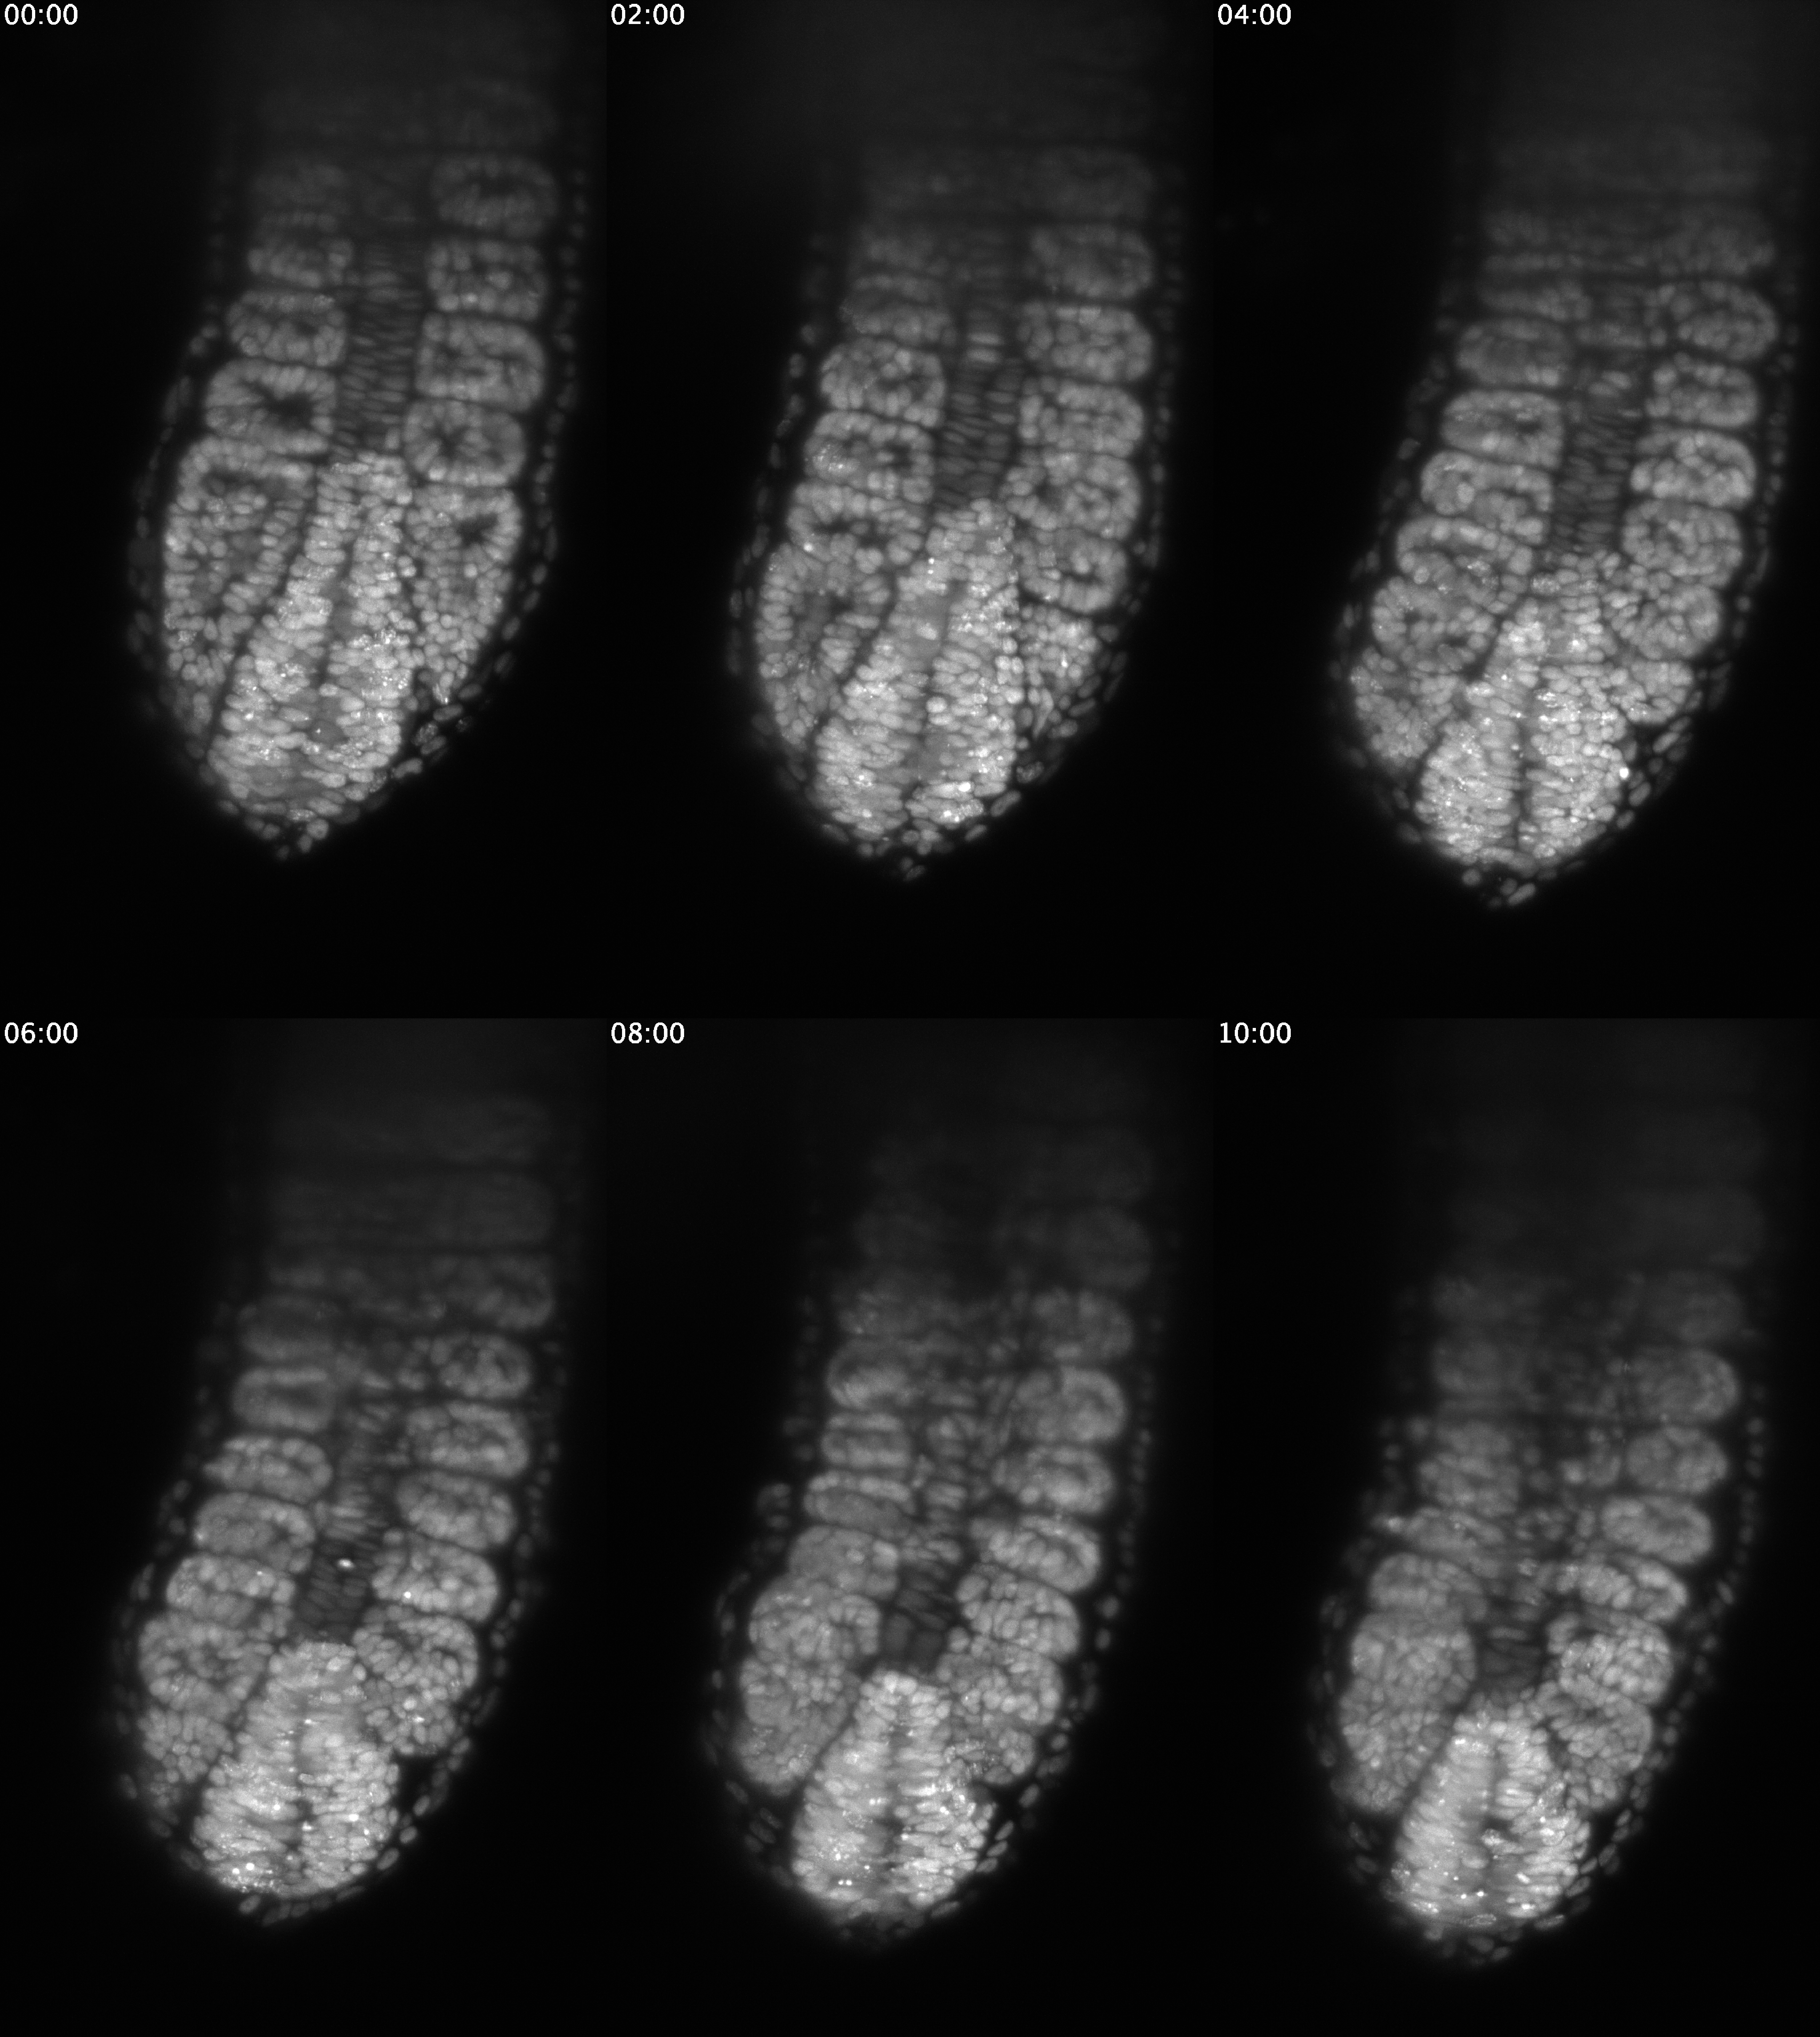
\includegraphics[width=1\linewidth]{figs/somites/ali_fish_seg_compiled} \hfill{}

\caption{Time-stamped images of somite segmentation in medaka, generated by Ali Seleit.}\label{fig:somite-seg-ali}
\end{wrapfigure}

The period of somite formation is controlled by a molecular oscillator, known as the `segmentation clock', which drives waves of gene expression in the Notch, fibroblast growth factor (FGF), and Wnt pathways, forming a signalling gradient that regresses towards the tail in concert with axis elongation (Gomez et al. 2008). Over the course of elongation, the wave period increases (i.e.~each somite takes longer to form), and the PSM progressively shrinks until it is exhausted, eventually terminating somite formation (Gomez et al. 2008).

It is not fully understood how the phase waves of the segmentation clock are initially established (Falk et al. 2022). Matsuda et al. (2020) found that period differences between mouse and human occur at the single-cell level (i.e.~not due to intercellular communication), and are driven by biochemical reaction speeds - specifically, mRNA and protein degradation rates, transcription and translation delays, and intron and splicing delays. To identify the genetic basis of these biochemical differences, our collaborators Ali Seleit and Alexander Aulehla at EMBL-Heidelberg used a CRISPR-Case9 knock-in approach (Seleit, Aulehla, and Paix 2021) to establish a medaka \emph{Cab} strain with an endogenous, fluorescing reporter gene (Her7-Venus) for the oscillation signalling pathway. This method allows them to image somite formation and extract quantitative measures for segmentation clock dynamics.

In medaka, it is known that the southern Japanese \emph{Cab} strain and the northern Japanese \emph{Kaga} strain have divergent somite periodicity, where \emph{Kaga}'s tends to be faster, and \emph{Cab}'s slower (\textbf{Figure \ref{fig:F0-Cab-Kaga-HdrR}}).



\begin{wrapfigure}{R}{0.5\textwidth}

\hfill{}\includegraphics[width=1\linewidth]{figs/somites/ali_period_F0_Cab_Kaga} 

\caption{Comparison of period for three inbred medaka strains (\emph{Cab}, \emph{Kaga} and \emph{HdrR}). Kaga's period is lower, and therefore it takes less time to form each somite than \emph{Cab}. Figure generated by Ali Seleit.}\label{fig:F0-Cab-Kaga-HdrR}
\end{wrapfigure}

Our collaborators accordingly set up a one-way F2 cross experiment as described in Chapter \ref{MIKK-F2-cross}, using the reporter-carrying \emph{Cab} strain and the \emph{Kaga} strain as the parental F0 strains, in order to identify genetic loci associated with these differences in clock dynamics. They inter-crossed the hybrid F1 generation to create a sample of 622 F2 individuals, imaged the developing embryos of these F2 samples, and used pyBOAT (Schmal, Mönke, and Granada 2022) to extract the oscillation features during somite development. \textbf{Figure \ref{fig:somite-period-ali}} shows a series of raw images used by pyBOAT to track the elongation of a medaka tail during somitogenesis, with the identified posterior tip of the embryo labelled with a blue circle.



\begin{wrapfigure}{L}{0.5\textwidth}

\includegraphics[width=1\linewidth]{figs/somites/ali_compiled_somite_elong} \hfill{}

\caption{Screenshots of vertebral elongation in an F2 individual captured by Ali Seleit during imaging. The blue circle represents the point tracked by pyBOAT over time, generating the quantitative phenotype data on period development used in this study.}\label{fig:somite-period-ali}
\end{wrapfigure}

\hypertarget{behaviour}{%
\subsection{Behaviour}\label{behaviour}}

In \textbf{Chapters \ref{Pilot-chap}} and \textbf{\ref{MIKK-F2-chap}} I use medaka as a model organism to explore social genetic effects on bold-type behaviours. Behaviour is a complex trait that is affected by both genes and environment, and for social animals such as humans and medaka, one's social environment is considered likely to constitute a large component of the environmental effect (Ruzzante and Doyle 1990; Young 2008). Apart from social aspects, an organism must face many ``hostile forces of nature'' throughout its life (Buss 1991; Darwin 1859), such as food shortages, predation, harsh climate, and diseases. Adaptive behaviours allow individuals to navigate such dangers and maximise the likelihood of their survival at both the individual and population level (Lima and Dill 1990).

Boldness-shyness is thought to be a fundamental axis of behavioural variation in many species, with an obvious causal relationship to an individual's likelihood of survival, and consequently with natural selection at the population level (Sloan Wilson et al. 1994). It represents an evolutionary trade-off between acquiring benefits (in terms of food or mates) and avoiding harms (in terms of predators or conspecific competitors), with each situation accompanied by its own optimal degree of risk (Lima and Dill 1990). It is both heritable (Svartberg 2002; Culum Brown, Burgess, and Braithwaite 2007), and subject to change following different life experiences or under different environmental conditions (Culum Brown, Burgess, and Braithwaite 2007).

{[}OPEN FIELD AND NOVEL OBJECT IS A GENERIC PARADIGM, NOT JUST FISH. CITE BAUD.{]}

Boldness-shyness has been studied extensively with fish. Shy individuals tend to react to novelty by reducing their activity and becoming more vigilant, whereas bold individuals show higher levels of activity and exploratory behaviour (C. Brown, Jones, and Braithwaite 2007). One assay commonly used to measure this behavioural domain is referred to as the `open field' assay, where fishes are observed while swimming freely in an experimental setting (C. Brown, Jones, and Braithwaite 2007; Laland, Krause, and Brown 2011; Lucon-Xiccato et al. 2022, 2020; Lucon-Xiccato and Bisazza 2017; Matsunaga and Watanabe 2010).

Another is the `novel object' assay, where a novel object is introduced to the fishes' environment to simulate a threat (C. Brown, Jones, and Braithwaite 2007; Schjolden, Stoskhus, and Winberg 2005; Wilson et al. 1993; Dominic Wright, Butlin, and Carlborg 2006; D. Wright et al. 2003). Where both assays were performed on the same fish, the behaviours exhibited were found to be correlated across assays, indicating that both were measuring the same boldness-shyness axis (C. Brown, Jones, and Braithwaite 2007). Both the open field and novel object assay also permit the measurement of habituation, where the response of the fish may change over time after growing accustomed to the new environment or object. Variation in the length of time the fish take to return to a more ``normal'' level of movement may indicate different levels of boldness (Laland, Krause, and Brown 2011).

\hypertarget{social-genetic-effects}{%
\subsubsection{Social genetic effects}\label{social-genetic-effects}}

The experiments described in \textbf{Chapters \ref{Pilot-chap}} and \textbf{\ref{MIKK-F2-chap}} are designed to simulataneously measure both the direct effect of an individual's genes on their behaviour, as we as the indirect effect of their social partner's genes on the focal individual's behaviour, which is also an environmental factor (Baud et al. 2017). Social genetic effects have been shown to exert influence on various traits in mice including anxiety, wound healing, immune function, and body weight (Baud et al. 2017), and various traits related to development and survival in many species of livestock (Ellen et al. 2014). However, in those studies the social interactions were maintained throughout development, and it is unclear whether social genetic effects can still exert influence on adaptive behaviours during discrete, time-limited interactions.

In \textbf{Chapter \ref{Pilot-chap}} I used a combined open-field and novel-object assay involving assaying pairs for fish, to determine: a) whether there were consistent differences in bold-shy behaviours exhibited by 5 established inbred strains of medaka fish (\emph{iCab}, \emph{HdrR}, and \emph{HO5} from southern Japan, and \emph{Kaga} and \emph{HNI} from northern Japan); and b) whether there were consistent differences in bold-shy behaviours exhibited by a given strain (\emph{iCab}) dependent on the strain that it was partnered with. The former was intended to measure the effect of an individual's own genes on its behaviour (a direct genetic effect), and the latter to measure the effect of the genes of the focal fish's tank partner on the behaviour of the focal fish (social genetic effect). Our experimental design allowed us to assess both direct and indirect effects on behaviour simultaneously, and to infer the degree to which variation in bold-shy behaviours is attributable to the differences in an individual's own genetics, the differences in the genetics of their social companions, and stochastic variation. A schema for the experimental plan is shown in \textbf{Figure \ref{fig:behavioural-schema}}.



\begin{figure}
\includegraphics[width=1\linewidth]{figs/pilot/experimental_schema} \caption{Schema for experimental plan. \emph{iCab}-\emph{iCab} pairings are the control condition. To explore direct genetic effects on behaviour, we compare the behaviours of test fishes from different lines, and infer that the differences between lines are caused by the differences in their genetics (direct genetic effects). To explore social genetic effects, we use the same data but turn our focus to the reference fish, and infer that the differences we observe between their behaviours are caused by the differences in their social environments, which are in turn driven by the different genetics in the test fish lines (social genetic effects).}\label{fig:behavioural-schema}
\end{figure}

In \textbf{Chapter \ref{MIKK-F2-chap}} I extend the behavioural analysis described in Chapter \ref{Pilot-chap} over the MIKK panel. I then identify the lines that diverged in both (a) their own behaviour; and (b) the level of transmission of their behaviour onto their \emph{\definecolor{iCab_424B4D}{HTML}{424B4D}\textcolor{iCab_424B4D}{iCab}} reference tank partner, and then use them as the parental strains in an F2 cross to attempt to identify the genetic variants associated with those differences.

\hypertarget{poor-transferability-of-polygenic-scores-to-diverse-human-populations}{%
\section{Poor transferability of polygenic scores to diverse human populations}\label{poor-transferability-of-polygenic-scores-to-diverse-human-populations}}

{[}CITE MIKE INOUYE{]}

\textbf{Chapter \ref{Fst-chap}} -- the final chapter of this thesis -- relates to the poor transferability of polygenic scores (\textbf{PRS}) derived from GWAS results when applied to non-European populations. Humans have long sought to use genetic information to predict an individual's likely value for a given trait, in our own species and in other organisms. As already discussed, an individual's phenotypic value at a given point in time is the product of complex interactions between their genome and their environment, beginning from embryonic development and continuing throughout their lifetimes. It is now clear that ``complex'' traits such as height, intelligence, and behaviour are highly polygenic, meaning that they are genetically influenced by hundreds or thousands of genetic variants, each exerting a small effect in one or the other direction along the trait's spectrum (Sella and Barton 2019).

A richer understanding of the cumulative effect of genetic variants on any trait allows for the prediction of the value that an individual is most likely to have for that trait. Of all human traits, diseases are particularly salient; in 2018, the global healthcare industry was valued at US\$8 trillion, and predicted to increase to US\$12 trillion by 2022 ({``The \$11.9 {Trillion Global Healthcare Market}: {Key Opportunities} \& {Strategies} (2014-2022) - {ResearchAndMarkets}.com''} 2019). This strong financial imperative complements the moral imperative to reduce suffering, together driving the question of how to use genetic information to improve human health.

Recent technological developments have made it possible to sequence human genomes at scale, and it is thought that by combining detailed genetic information with with other environmental and phenotypic information (such as lifestyle or clinical factors), clinicians could move towards the practice of ``precision medicine'', where interventions could be tailored to their patients' unique risk profiles (Wray, Goddard, and Visscher 2007). The use of genetic information to predict individuals' values for a trait of interest entails the construction of metrics known as ``polygenic scores'' (\textbf{PGS}). When the trait is a disease, PGS is commonly known as polygenic risk scores (\textbf{PRS}), or genetic risk profiling, but I use the term PGS to encompass both disease and non-disease traits.

\hypertarget{polygenic-scores-pgs-and-gwas}{%
\subsection{Polygenic Scores (PGS) and GWAS}\label{polygenic-scores-pgs-and-gwas}}

\hypertarget{pgs}{%
\subsubsection{PGS}\label{pgs}}

PGS using genetic information alone show modest yet reliable accuracy for the prediction of complex traits (Alicia R. Martin et al. 2019): the correlations between PGS and the trait value as measured by \(R^2\) have reached 0.24 for height (Yengo et al. 2018), and 0.12-0.16 for educational attainment (Okbay et al. 2022). PGS also improve predictions beyond non-genetic clinical models for a variety of health-related traits, including breast cancer (Maas et al. 2016), prostate cancer (Schumacher et al. 2018), and type I diabetes (Sharp et al. 2019). The predictive accuracy of PGS scores can be further improved by combining genetic information with lifestyle and clinical factors, as seen with cardiovascular disease (Khera et al. 2018; Kullo et al. 2016; Natarajan et al. 2017; Paquette et al. 2017; Tikkanen et al. 2013; Sun et al. 2021).

\hypertarget{gwas}{%
\subsubsection{GWAS}\label{gwas}}

Most GWAS have been performed with individuals of European ancestry, despite only constituting around 16\% of the present global population. Although the proportion of participants in GWAS from a non-European background increased from 4\% in 2009 to 16\% in 2016 (Popejoy and Fullerton 2016)), as of 2019, 79\% of all GWAS participants recorded in the GWAS Catalog were of European ancestry, and the proportion of non-European individuals has remained the same or reduced since late 2014 (Alicia R. Martin et al. 2019). This bias extends to PGS studies, where as of 2019, only 67\% of them included only participants of European ancestry, with another 19\% including only East Asian ancestry participants, and only 3.8\% with cohorts of African, Hispanic, or Indigenous ancestry (Duncan et al. 2019).

It is therefore unsurprising that PGS scores are far better at predicting disease risk in individuals of European ancestry than in those of non-European ancestry (Alicia R. Martin et al. 2017; Alicia R. Martin et al. 2019). Indeed, the predictive accuracy of PGS scores decays with genetic divergence of the GWAS ``independent'' or ``test'' sample, from the ``discovery'' or ``training'' sample, as established in both humans (Alicia R. Martin et al. 2017; Alicia R. Martin et al. 2019), and livestock (Clark et al. 2012; Habier et al. 2010; Pszczola et al. 2012).

Compared to PGS scores for those of European ancestry, PGS scores across multiple traits are \textasciitilde64-78\% less accurate for individuals of African ancestry, (Duncan et al. 2019; Alicia R. Martin et al. 2019), \textasciitilde50\% less accurate for individuals of East-Asian ancestry, and \textasciitilde37\% less accurate for individuals of South-Asian ancestry (Alicia R. Martin et al. 2019).

\hypertarget{contributors-to-pgs-non-transferability}{%
\subsection{Contributors to PGS non-transferability}\label{contributors-to-pgs-non-transferability}}

What explains this disparity in predictive value? A number of factors may be responsible, including:

\begin{enumerate}
\def\labelenumi{\arabic{enumi}.}
\item
  The failure of GWAS to identify causal variants that either do not exist or are not identifiable within the ``discovery'' sample, for both technological and methodological reasons (Alicia R. Martin et al. 2019);
\item
  The sample populations may differ in linkage disequilibrium (\textbf{LD}) -- the correlation structure of the genome -- which would change the estimated effect sizes of the causal variants, even when the causal variants themselves are the same (Alicia R. Martin et al. 2019);
\item
  Allele frequencies of the causal variants, and the distribution of the effect sizes of the causal variants, may differ between populations (Alicia R. Martin et al. 2017; Scutari, Mackay, and Balding 2016); and
\item
  The environments and demographies of populations tend to differ. Such differences are often correlated with genetic divergence due to geography, making it difficult to determine whether the associations are driven by the differences between population in their genetics, or their environments (Alicia R. Martin et al. 2019; Kerminen et al. 2019).
\end{enumerate}

The first three factors can degrade predictive performance even in the absence of biological and environmental differences. On the other hand, environmental and demographic differences can drive forces of natural selection can in turn drive differences in causal genetic architecture (Alicia R. Martin et al. 2019).

I will discuss each of these factors in turn before addressing point (3) in this analysis.

\hypertarget{fst-discovery-sec}{%
\subsubsection{Technological and methodological limitations of GWAS}\label{fst-discovery-sec}}

The power to discover a causal variant through GWAS depends on the variant's effect size and frequency in the study population (Alicia R. Martin et al. 2019; Sham et al. 2000). That is to say, the stronger the variant's effect, or the more common it is, the more likely it is to be discovered. Rare variants tend to have stronger effect sizes (Watanabe et al. 2019), likely due to purifying selection (Park et al. 2011), and tend not to be shared across populations (Gravel et al. 2011; 1000. G. P. Consortium et al. 2015). This is particularly relevant for African populations, as they have a much greater level of genetic variance than other populations due to the human species having originated on that continent (1000. G. P. Consortium et al. 2015). Therefore, if GWAS aren't performed on diverse populations, PGS can't take into account the rare variants present in non-European populations that are likely to exert stronger effects on the trait of interest. There are also several other issues that can affect the discoverability of causal variants through GWAS, including the technology used for genotyping, the selection of the cohort, and the necessary exclusion of genotypic outliers.
With respect to genotyping technologies, GWAS often use data from SNP microarrays. These do not sequence the whole genome, but rather a selection (from several hundred thousand to millions) of genetic markers intended to present \emph{common} genetic variation (Porcu et al. 2013), which accordingly tend to neglect rare genetic variants (Uffelmann et al. 2021). To increase the density of genotypes, which would increase the likelihood of refining the association signal and identifying causal variants, researchers often ``impute'' variants that aren't sequenced directly (Porcu et al. 2013). The imputation process involves ``phasing'' the study genotypes onto the genotypes of a ``reference panel'' (McCarthy et al. 2016). However, if the reference panel does not sufficiently represent the population in the study sample, they are likely to miss or incorrectly impute those genotypes (Alicia R. Martin et al. 2019). Again, this is particularly problematic for African populations.

The lack of representation of rare variants in SNP microarrays can be overcome by using next-generation sequencing technologies such as whole-genome sequencing (\textbf{WGS}) and whole-exome sequencing (\textbf{WES}). (The former seeks to sequence the full genome, and the latter of only targets the coding regions of the genome.) These methods are more expensive than SNP microarrays, which hinders their widespread use at scale, and although their costs are continuing to decrease rapidly, there is a question as to whether they return a proportionate benefit in all use cases (Schwarze et al. 2018).

A second limitation is the selection of GWAS cohorts, which can introduce selection and collider biases (Uffelmann et al. 2021). For instance, the UK Biobank, which contains genetic and phenotypic data on 500,000 participants who volunteered for inclusion between 2006 and 2010, tend to be older, female, healthier, and wealthier than non-participants (Fry et al. 2017). This creaties the possibility of confounding genetic associations with environmental factors, which I discuss further in \ref{fst-env-sec} below.

A third limitation is the ``quality control'' step that is required during the GWAS process (Uffelmann et al. 2021). To avoid confounding from population stratification, which can lead to overestimated heritability and biased PGS, GWAS cohorts are filtered to include only those with similar ancestries -- or relative genetic homogeneity -- by clustering individuals through principal component analysis (\textbf{PCA}) of their genotypes, and excluding outliers. I elaborate on the issue of population stratification in section \ref{fst-env-sec} below, but at present, a statistical model for GWAS that can include cohorts with diverse ancestries without the risk of serious confounding is yet to be developed (Jeremy J. Berg et al. 2019).

\hypertarget{differences-in-ld}{%
\subsubsection{Differences in LD}\label{differences-in-ld}}

Because GWAS SNP markers are often not the causal variants themselves, but merely in physical proximity to them, the estimated effect size of a SNP marker depends on the extent to which it is in LD with the causal variant (Mostafavi et al. 2020; Pritchard and Przeworski 2001). To illustrate the problem, if a SNP has an LD \(r^2\) with a causal variant of 0.8 in the discovery population and 0.6 in the target population, it would explain 25\% = (1 - 0.6/0.8) less trait variation in the target population, and would therefore be less predictive (Ying Wang et al. 2020).

These differences in effect-size estimates may typically be small for most regions of the genome, but as PGS sum across all such effects, they aggregate these population differences (Alicia R. Martin et al. 2019; Jeremy J. Berg et al. 2019). Previous empirical and simulation studies have shown that accuracy of PGS scores decay with increased genetic differentiation (\(F_{ST}\) -- described below in \ref{Fst-descr}) and LD differences between populations (Habier et al. 2010; Pszczola et al. 2012; Scutari, Mackay, and Balding 2016; Ying Wang et al. 2020). The issue may be addressed to a degree by using LD information from an external reference panel as a prior to infer the posterior mean effect size of a genetic variant -- Vilhjálmsson et al. (2015) demonstrated through simulations that this could improve PGS predictive accuracy. Yet the most appropriate means of deal with differences between populations in LD remains an active area of research (Duncan et al. 2019).

\hypertarget{differences-in-allele-frequencies}{%
\subsubsection{Differences in allele frequencies}\label{differences-in-allele-frequencies}}

Causal variants can differ in both frequency and effect size between different ancestry groups, e.g.~for lactase persistence (S'egurel and Bon 2017), or skin pigmentation (Adhikari et al. 2019). If a causal allele is rare in the GWAS discovery population, even if it is discovered (see \ref{fst-discovery-sec}), it is likely to have noisy effect size estimates, and therefore likely to inaccurately estimate its effect size in a different population where it exists at a higher frequency.

Differences in allele frequencies between populations can arise through random genetic drift, or be driven by selective pressures towards the trait optima for a given environment (Harpak and Przeworski 2021). However, evolutionary biologists have found that differences between populations in the mean values for traits tend to occur through small, coordinated shifts in their allele frequencies (Jeremy J. Berg et al. 2019; Edge and Coop 2019). In Chapter \ref{Fst-chap}, I explore the differences in allele frequencies across populations for all polygenic traits in the GWAS Catalog, and confirm that with few exceptions -- including skin pigmentation, and HIV viral load -- the differences in allele frequencies between populations tends to be small.

\hypertarget{fst-env-sec}{%
\subsubsection{Differences in environment}\label{fst-env-sec}}

Genes continuously interact with each other (GxG, or ``epistasis'' (Gros, Le Nagard, and Tenaillon 2009)), the genes of one's parents (``genetic nurture'', Kong et al. (2018)) or social companions (``social genetic effects'') (Domingue et al. 2018; Baud et al. 2017),\footnote{As also explored in Chapters \ref{Pilot-chap} and \ref{MIKK-F2-chap}} and the wider non-genetic environment (GxE).

The respective contributions of genetics and environment to traits with social value -- such as intelligence -- is highly contentious, especially when there are apparent differences between populations in the mean values for those traits. PGS measure the proportion of variance within a population that is explained by genetics. Because PRS summarises a \emph{proportion} of the total variance, when studying a population that is subject to greater environmental variation, the variance attributable to genetic factors will proportionately reduce. The corollary being that when studying a population where the environment is held constant, the proportion of variance for that trait that is explained by genetic factors will approach 1. Therefore, increases in the amount of environmental variance that a population is exposed to will reduce the accuracy of PGS predictions when applied to that population.

Different environments are also often correlated with population structure (Jeremy J. Berg et al. 2019). For example, in East Asia, there is a greater proportion of individuals of East-Asian ancestry than there is of European ancestry, and \emph{vice versa} in Europe. Those East-Asian individuals will therefore tend to share more of their genetic background with each other than with Europeans, and that population structure will be correlated with the different environments that exist in East Asia compared to Europe. This makes it difficult to determine whether it is the differences in their environments or the differences in their genetics that is driving the discrepancies between the mean values for traits between those populations. These complexities are unlikely to be resolved in the near future, which makes it attractive to turn to model organisms to address more basic biological questions regarding GxE in relation to complex traits (Andersson and Georges 2004), as we have done with respect to behaviour in Chapters \ref{Pilot-chap} and \ref{MIKK-F2-chap}.

\hypertarget{Fst-descr}{%
\subsection{\texorpdfstring{\(F_{ST}\)}{F\_\{ST\}}}\label{Fst-descr}}

The widely-used fixation index (\(F_{ST}\)) was introduced independently by Sewall Wright (S. Wright 1949) and Gustave Malécot (Mal'ecot 1948) as a metric for measuring the genetic diversity between populations.\footnote{In Wright's notation, \(F\) refers to ``fixation'' of an allele, and \(_{ST}\) refers to ``subpopulations within the total population''.} It quantifies the relative variance in allele frequency between groups compared to within groups, reflecting the combined effects of genetic drift, migration, mutation, and selection (Holsinger and Weir 2009). The metric ranges from 0 to 1, where loci with high \(F_{ST}\) values -- that is, loci with a large relative between-group variance in allele frequencies -- may have been subject to selection or different demographic processes (Holsinger and Weir 2009). The metric has customarily been used to identify regions of the genome have been subject to diversifying selection (Akey et al. 2002; Guo, Dey, and Holsinger 2009; Bruce S. Weir et al. 2005).

\hypertarget{genomic-variations-in-the-mikk-panel-mikk-genomes-chap}{%
\chapter[Genomic variations in the MIKK panel \{\#MIKK-genomes-chap\}]{\texorpdfstring{Genomic variations in the MIKK panel \{\#MIKK-genomes-chap\}\footnote{This project was carried out in collaboration with Felix Loosli's group at the Karlsruhe Institute of Technology (KIT), and Joachim Wittbrodt's group in the Centre for Organismal Studies (COS) at the University of Heidelberg. This chapter sets out my contributions to Fitzgerald et al. (2022) and Leger et al. (2022), which were published as companion papers in the journal \emph{Genome Biology} to introduce the MIKK panel to the scientific community, and describe the genetic characteristics of the MIKK panel that would make it a useful resource for other researchers who wish to explore the genetics of quantitative traits in vertebrates. I am joint-first author on both papers.}}{Genomic variations in the MIKK panel \{\#MIKK-genomes-chap\}}}\label{genomic-variations-in-the-mikk-panel-mikk-genomes-chap}}

\hypertarget{the-medaka-inbred-kiyosu-karlruhe-mikk-panel}{%
\section{The Medaka Inbred Kiyosu-Karlruhe (MIKK) panel}\label{the-medaka-inbred-kiyosu-karlruhe-mikk-panel}}

I introduced the MIKK panel in section \ref{MIKK-background} of the previous chapter, and here I describe several of its genomic characteristics that are relevant to its utility for the genetic mapping of complex traits. These include a visualisation of the inbreeding trajectory of the panel (section \ref{inbreeding-sec}), an exploration of the evolutionary history of the MIKK panel's founding population (section \ref{introgression-sec}), measurement of the levels of homozygosity across the panel (section \ref{nuc-div}), an assessment of the panel's allele-frequency distribution and rate of linkage disequilibrium (LD) decay (section \ref{ld-decay-sec}), and a characterisation of the structural variants present in a smaller sample of lines using Oxford Nanopore long-read sequencing data (section \ref{mikksv-sec}).

\hypertarget{genomic-characterisation-of-the-mikk-panel}{%
\section{Genomic characterisation of the MIKK panel}\label{genomic-characterisation-of-the-mikk-panel}}

\hypertarget{non-sib-calls}{%
\subsection{MIKK panel DNA sequence dataset}\label{non-sib-calls}}

In 2018, our collaborators sequenced 79 of the 80 extant MIKK panel lines -- together with several wild Kiyosu samples and individuals from the established \emph{iCab} medaka strain -- from male brain samples using Illumina short-read sequencing technology. Tomas Fitzgerald from the Birney Group at EMBL-EBI then aligned these sequences to the \emph{HdrR} medaka reference ({``Index of /Pub/Release-104/Fasta/Oryzias\_latipes/Dna''} n.d.) and called variants to produce the \textbf{MIKK Illumina call set} in the form of a .vcf file containing single nucleotide polymorphism (SNP) and small insertion-deletion (INDEL) calls for each line. To avoid allele frequency biases introduced by the 16 pairs/triplets of ``sibling lines'' (see \ref{inbreeding-sec}), I removed each pair's arbitrarily-labelled second sibling line from the variant call set, leaving 63 MIKK panel lines (\textbf{MIKK non-sibling call set}), and used only those calls for the analyses in sections \ref{nuc-div} and \ref{ld-decay-sec} below.

We also performed a pilot study on 12 MIKK panel lines by sequencing DNA from brain samples using Oxford Nanopore Technologies (ONT) long-read sequencing technology. Adrien Leger from the Birney Group at EMBL-EBI then aligned these sequences to the \emph{HdrR} medaka reference ({``Index of /Pub/Release-104/Fasta/Oryzias\_latipes/Dna''} n.d.), and called variants to produce the \textbf{MIKK ONT call set} in the form of a .vcf file containing structural variants calls for each line with tags for insertions (INS), deletions (DEL), duplications (SUP), inversions (INV) and translocations (TRA). The work described below used these variant call sets as the primary datasets.

\hypertarget{inbreeding-sec}{%
\subsection{Assessing the inbreeding trajectory of the MIKK panel}\label{inbreeding-sec}}

The MIKK panel was bred from a wild population of medaka found in the Kiyosu area near Toyohashi, Aichi Prefecture, in southern Japan.(Spivakov et al. 2014) From this wild population, the Loosli Group at KIT set up random crosses of single mating pairs to create 115 `founder families'. For each founder family, they then set up between two and five single full-sibling-pair inbreeding crosses, which resulted in 253 F1 lines. Lines derived from the same founder family are referred to as `sibling lines'. Over the course of the next eight generations of inbreeding, they used only one mating pair per line. I generated \textbf{Fig. \ref{fig:InbreedingFigure}A} and \textbf{B} from the inbreeding data provided by the Loosli Group. \textbf{Fig. \ref{fig:InbreedingFigure}A} shows the number of lines that survived over the course of the first 14 generations of the inbreeding program, and the various causes for the termination of other lines. \textbf{Fig. \ref{fig:InbreedingFigure}B} shows the average fecundity levels of the surviving lines at generation F16.



\begin{figure}
\includegraphics[width=1\linewidth]{figs/mikk_genome/20211213_final_figure} \caption{Inbreeding, fecundity and eye size in the MIKK panel lines. \textbf{A}: Status of all MIKK panel lines during the first 14 generations of inbreeding, showing cause of death for non-extant lines. \textbf{B}: Average fecundity of MIKK panel lines in generation F16, as measured during peak egg production in July 2020. \textbf{C}: Distribution of mean relative eye size for female and male medaka across all MIKK panel lines.}\label{fig:InbreedingFigure}
\end{figure}

In addition, the Birney Group at EMBL-EBI generated morphometric data for the MIKK panel lines to demonstrate the distribution of physical phenotypes across the MIKK panel. I used this data on relative eye diameters to generate \textbf{Fig. \ref{fig:InbreedingFigure}C}, and as we can see, the trait has a roughly normal distribution, with minimal differences in the mean between sexes. I also computed this trait's broad-sense heritability \(\eta^2_{(partial)} = \hat{H^2} = SS_{line} / (SS_{line} + SS_{residuals}) =\) 0.56. This value is on the higher range of heritability estimates for morphological traits across different species inluding mouse and human (Visscher, Hill, and Wray 2008; Claes et al. 2018; Weinberg, Cornell, and Leslie 2018), and indicates that the majority of variance observed across the panel is driven by differences between lines in their genetics. This in turn makes the MIKK panel a promising resource for discovering the genetic variants that create such differences.

\hypertarget{levels-of-homozygosity}{%
\subsection{Levels of homozygosity}\label{levels-of-homozygosity}}

To roughly assess whether the inbreeding process resulted in high levels of homozygosity in the MIKK panel, for each line I extracted from the MIKK Illumina call set all non-missing, biallelic calls (both SNPs and indels)with \emph{bcftools} (Danecek et al. 2021), counted the number of SNPs within non-overlapping, 5-kb bins, and calculated the proportion of SNPs within each bin that were homozgyous. To provide an example of the levels of homozygosity in the MIKK panel, \textbf{Figure \ref{fig:circos-18-2}} is a circos plot generated with circlize (Gu et al. 2014) for the MIKK panel line 18-2, featuring the proportion of homozygous SNPs per 5-kb bin (pink), and the total number of SNPs in each bin (yellow). With few exceptions, almost all 5-kb bins across the genome contain a very high proportion of homozygous variants, and all other MIKK panel lines show similar levels of homozygosity. Although there are more sophisticated means of measuring homozygosity -- for example, by using a Hidden Markov Model to separate out regions of residual homozygosity\footnote{As described in Fitzgerald et al. (2022).} -- this confirms that the breeding program was successful in establishing a panel of inbred lines with levels of homozygosity comparable to established medaka strains that have been inbred for dozens of generations, such as the \emph{iCab} strain at generation F24 which was sequenced with the MIKK panel (\textbf{Figure \ref{fig:circos-iCab-F24}}).



\begin{figure}
\includegraphics[width=1\linewidth]{figs/mikk_genome/circos/18-2} \caption{Proportion of homozygous SNPs within 5 kb bins in the MIKK panel line 18-2 (pink), and number of SNPs in each bin (yellow).}\label{fig:circos-18-2}
\end{figure}



\begin{figure}
\includegraphics[width=1\linewidth]{figs/mikk_genome/circos/iCab_F24} \caption{Proportion of homozygous SNPs within 5 kb bins in the previously established \emph{iCab} strain at generation F24 (dark grey), and number of SNPs in each bin (yellow).}\label{fig:circos-iCab-F24}
\end{figure}

\hypertarget{nuc-div}{%
\subsection{Nucleotide diversity}\label{nuc-div}}

We also sought to assess the levels of genetic diversity in the MIKK panel, and to compare them with the levels of genetic diversity present in the wild Kiyosu population. If the levels were similar, it would confirm that the MIKK panel provided a reasonable representation of the variation present in its originating population, and that any selection for loci associated with domestication was not widespread across the genome. As a means of assessing genetic diversity in the MIKK panel, I calculated the widely-used measure of `nucleotide diversity' (\(\hat{\pi}\)) (Nei and Li 1979) within 500-kb non-overlapping windows across the genome of the 63 lines in the MIKK non-sibling call set (see \ref{non-sib-calls}), and compared this to the nucleotide diversity in 7 wild medaka from the same Kiyosu population from which the MIKK panel was derived. Mean and median nucleotide diversity in both the MIKK panel and wild Kiyosu medaka were close to 0, and slightly higher in the MIKK panel (mean: MIKK = 0.0038, wild = 0.0037; median: MIKK = 0.0033, wild = 0.0031). This may have been caused by the smaller sample size of wild Kiyosu medaka, as mean \(\hat{\pi}\) for a random sample of 7 MIKK lines dropped to 0.0037, although it is unexpected that the highly-inbred MIKK lines have similar levels of \(\hat{\pi}\) to wild Kiyosu individuals. The patterns of varying nucleotide diversity across the genome are shared between the MIKK panel and wild Kiyosu medaka, where regions with high levels of repeat content tend to have higher nucleotide diversity (r = 0.386, \(p\) \textless{} 0.001) (\textbf{Fig. \ref{fig:NucleotideDiversity}}). I also calculated \(\hat{\pi}\) for each line individually, and as expected, levels of \(\hat{\pi}\) around the (XX/XY) sex determination region of 1:\textasciitilde16-17 Mb are elevated in all lines relative to the consistently low levels found in most other chromosomes.



\begin{figure}
\includegraphics[width=1\linewidth]{figs/mikk_genome/supp_01_pi_circos} \caption{Circos plot with nucleotide diversity (\(\hat{\pi}\)) calculated within 500-kb non-overlapping windows for 63 non-sibling lines from the MIKK panel (\emph{green}) and 7 wild Kiyosu medaka samples from the same originating population (\emph{purple}); proportion of sequence classified as repeats by RepeatMasker (\emph{blue}); and mean mapping quality (\emph{pink}).}\label{fig:NucleotideDiversity}
\end{figure}

The higher level of \(\hat{\pi}\) observed within specific regions on several chromosomes -- such as chromosomes 2, 11, and 18 -- correspond closely to the regions we identified as containing large (\textgreater250 kb) inversions that appear to be shared across at least some of the MIKK panel (\textbf{Fig. \ref{fig:SVInvs}}). These regions are also enriched for large deletions and duplications.(Leger et al. 2022) Inversions cause permanent heterozygosity (Hoffmann, Sgr`o, and Weeks 2004), and duplications and deletions may have increased the density of called SNPs in these regions (Fredman et al. 2004), so the observed depressions in homozygosity at these loci may be the result of such large structural variants that are present in the MIKK panel's genomes.

Overall, this analysis confirms that the MIKK panel shows similar levels of homozygosity compared to classical laboratory inbred medaka strains, and possesses a strong increase in isogenic genotypes compared to wild medaka from the original wild population.



\begin{figure}
\includegraphics[width=1\linewidth]{figs/mikk_genome/20210224_sv_invs_lines} \caption{Inversions identified in 9 MIKK panel lines using a combination of Oxford Nanopore Technologies long-read and Illumina short-read sequences (see Chapter \ref{mikksv-sec} below).}\label{fig:SVInvs}
\end{figure}

\hypertarget{introgression-sec}{%
\subsection{Introgression with northern Japanese and Korean medaka populations}\label{introgression-sec}}

There is an o explore the evolutionary history of the MIKK panel's founding population, we sought to determine whether there was evidence of introgression between that southern Japanese population, and northern Japanese and Korean medaka populations. To this end, I used the 50-fish multiple alignment from Ensembl release 102 to obtain the aligned genome sequences for the established medaka inbred lines \emph{HdrR} (southern Japan), \emph{HNI} (northern Japan), and \emph{HSOK} (Korea), as well as the most recent common ancestor of all three strains.({``Index of /Pub/Release-102/Emf/Ensembl-Compara/Multiple\_alignments/50\_fish.epo/''} n.d.) Using the phylogenetic tree provided with the dataset, and the \emph{ape} R package,(Paradis and Schliep 2019) I identified the most recent common ancestor of those three strains. For each locus with a non-missing base for \emph{HdrR}, I assigned the allele in that ancestral sequence as the `ancestral' allele, and the alternative allele as the `derived' allele, and then combined that dataset with the MIKK Illumina call set and variant calls for the southern Japanese \emph{iCab} strain (see \ref{non-sib-calls}).

I then carried out an ABBA BABA analysis to calculate a modified `admixture proportion' statistic \(\hat{f}_d\)(S. H. Martin, Davey, and Jiggins 2015) as a measure of the proportion of shared genome in 500-kb sliding windows between the MIKK panel and either \emph{iCab}, \emph{HNI}, or \emph{HSOK} (\textbf{Fig. \ref{fig:ABBABABA}}), using the scripts provided by the first author of S. H. Martin, Davey, and Jiggins (2015) on their GitHub page.(martin {[}2016{]} 2022)



\begin{figure}
\includegraphics[width=1\linewidth]{figs/mikk_genome/07_introgression} \caption{\textbf{Figure 2}: ABBA-BABA analysis. \textbf{A}. Phylogenetic tree generated from the Ensembl release 102 50-fish multiple alignment, showing only the medaka lines used in the ABBA-BABA analysis. \textbf{B}. Schema of the comparisons carried out in the ABBA-BABA analysis. \textbf{C}. Circos plot comparing introgression (\(\hat{f}_d\)) between the MIKK panel and either \emph{iCab} (yellow), \emph{HNI} (orange), or \emph{HSOK} (purple), calculated within 500-kb sliding windows using a minimum of 250 SNPs per window.}\label{fig:ABBABABA}
\end{figure}

Based on the genome-wide mean \(\hat{f}_d\), the MIKK panel shares approximately 25\% of its genome with \emph{iCab}, 9\% with \emph{HNI}, and 12\% with \emph{HSOK}. These results provide evidence that the MIKK panel's originating population has more recently introgressed with medaka from Korea than with medaka from northern Japan. This supports the findings in Spivakov et al. (2014), where the authors found little evidence of significant interbreeding between southern and northern Japanese medaka since the populations diverged. Although the proportional difference between \emph{HNI} and \emph{HSOK} is small, this further supports the general finding that northern and southern Japanese medaka strains show low levels of interbreeding that may be a result of geographical isolation or genome divergence.(Katsumura et al. 2019)

\hypertarget{ld-decay-sec}{%
\subsection{LD decay}\label{ld-decay-sec}}

I analysed the MIKK panel's allele frequency distribution and linkage disequilibrium (LD) structure to assess their likely effects on genetic mapping. To remove allele-frequency biases introduced by the presence of sibling lines in the MIKK panel, I used only the MIKK non-sibling call set (see Chapter \ref{non-sib-calls}).

To assess how accurately one may be able to map genetic variants using the MIKK panel relative to a human dataset, I compared the MIKK panel's minor allele frequency (MAF) distribution and LD structure against that of the 2,504 humans in the 1KG Phase 3 release.({``A Global Reference for Human Genetic Variation''} 2015) To prepare the \textbf{``1KG call set''}, I first downloaded the .vcf files for each autosome from the project's FTP site (\url{ftp://ftp.1000genomes.ebi.ac.uk/vol1/ftp/release/20130502/}), then merged them into a single VCF using GATK.(McKenna et al. 2010) I then used PLINK(Chang et al. 2015; Purcell and Chang, n.d.) to calculate the minor allele frequencies for all non-missing, biallelic SNPs in both the MIKK non-sibling and IKG call sets (\emph{N} SNPs = 16,395,558 and 81,042,381 respectively) (\textbf{Fig. \ref{fig:LDdecay}A}). As expected, the 1KG and MIKK panel calls are similarly enriched for low-frequency variants, albeit to a lesser extent in the MIKK panel, which is likely due to its smaller sample size.

To determine the rate of LD decay in the MIKK panel and compare it to that in the 1KG sample, for both the MIKK non-sibling and 1KG call sets, I used PLINK to compute \(r^2\) on each autosome for all pairs of non-missing, biallelic SNPs with MAF \(>\) 0.10 within 10 kb of one another (for 1KG and the MIKK panel respectively \textasciitilde{} 5.5M and \textasciitilde{} 3M SNPs, with a total number of pairwise \(r^2\) observations of 204,152,922 and 146,785,673). I then grouped the \(r^2\) observations for each pair of SNPs based on their distance from one another into non-overlapping bins of 100 bp in length, and calculated the mean \(r^2\) in each of those bins to generate \textbf{Fig. \ref{fig:LDdecay}B} using the mean \(r^2\) and left boundary of each bin.



\begin{figure}
\includegraphics[width=1\linewidth]{figs/mikk_genome/08_ld_decay} \caption{Minor allele frequency distributions and LD decay for biallelic, non-missing SNPs in the 1000 Genomes Phase 3 variant calls (N = 2,504) (1KG), and the MIKK panel Illumina-based calls excluding one of each pair of sibling lines (N = 63), across all autosomes (1KG: chrs 1-22; MIKK: chrs 1-24). \textbf{A}: Histogram of allele frequencies in the 1KG and MIKK panel calls. \textbf{B}: LD decay for each autosome, calculated by taking the mean \(r^2\) of pairs of SNPs with MAF \(>\) 0.1 within non-overlapping 100 bp windows of distance from one another, up to a maximum of 10 kb. LD decays faster on chromosome 2 for the MIKK panel due to its higher recombination rate.}\label{fig:LDdecay}
\end{figure}

Based on the 1KG calls under these parameters, LD decays in humans to a mean \(r^2\) of around 0.2-0.35 at a distance of 10 kb, whereas the MIKK panel reaches this level within 1 kb, with a mean \(r^2\) of 0.3-0.4 at a distance of \textasciitilde100 bp. This implies that when a causal variant is present in at least two lines in the MIKK panel, one may be able to map causal variants at a higher resolution than in humans. We note that LD decays faster in chromosome 2 of the MIKK panel relative to the other chromosomes. This suggests that it has a much higher recombination rate, which is consistent with the linkage map described in Naruse et al. (2000), showing a higher genetic distance per Mb for this chromosome. This higher recombination rate in chromosome 2 may in turn be caused by its relatively high proportion of repeat content (\textbf{Fig. \ref{fig:repeats}}).



\begin{figure}
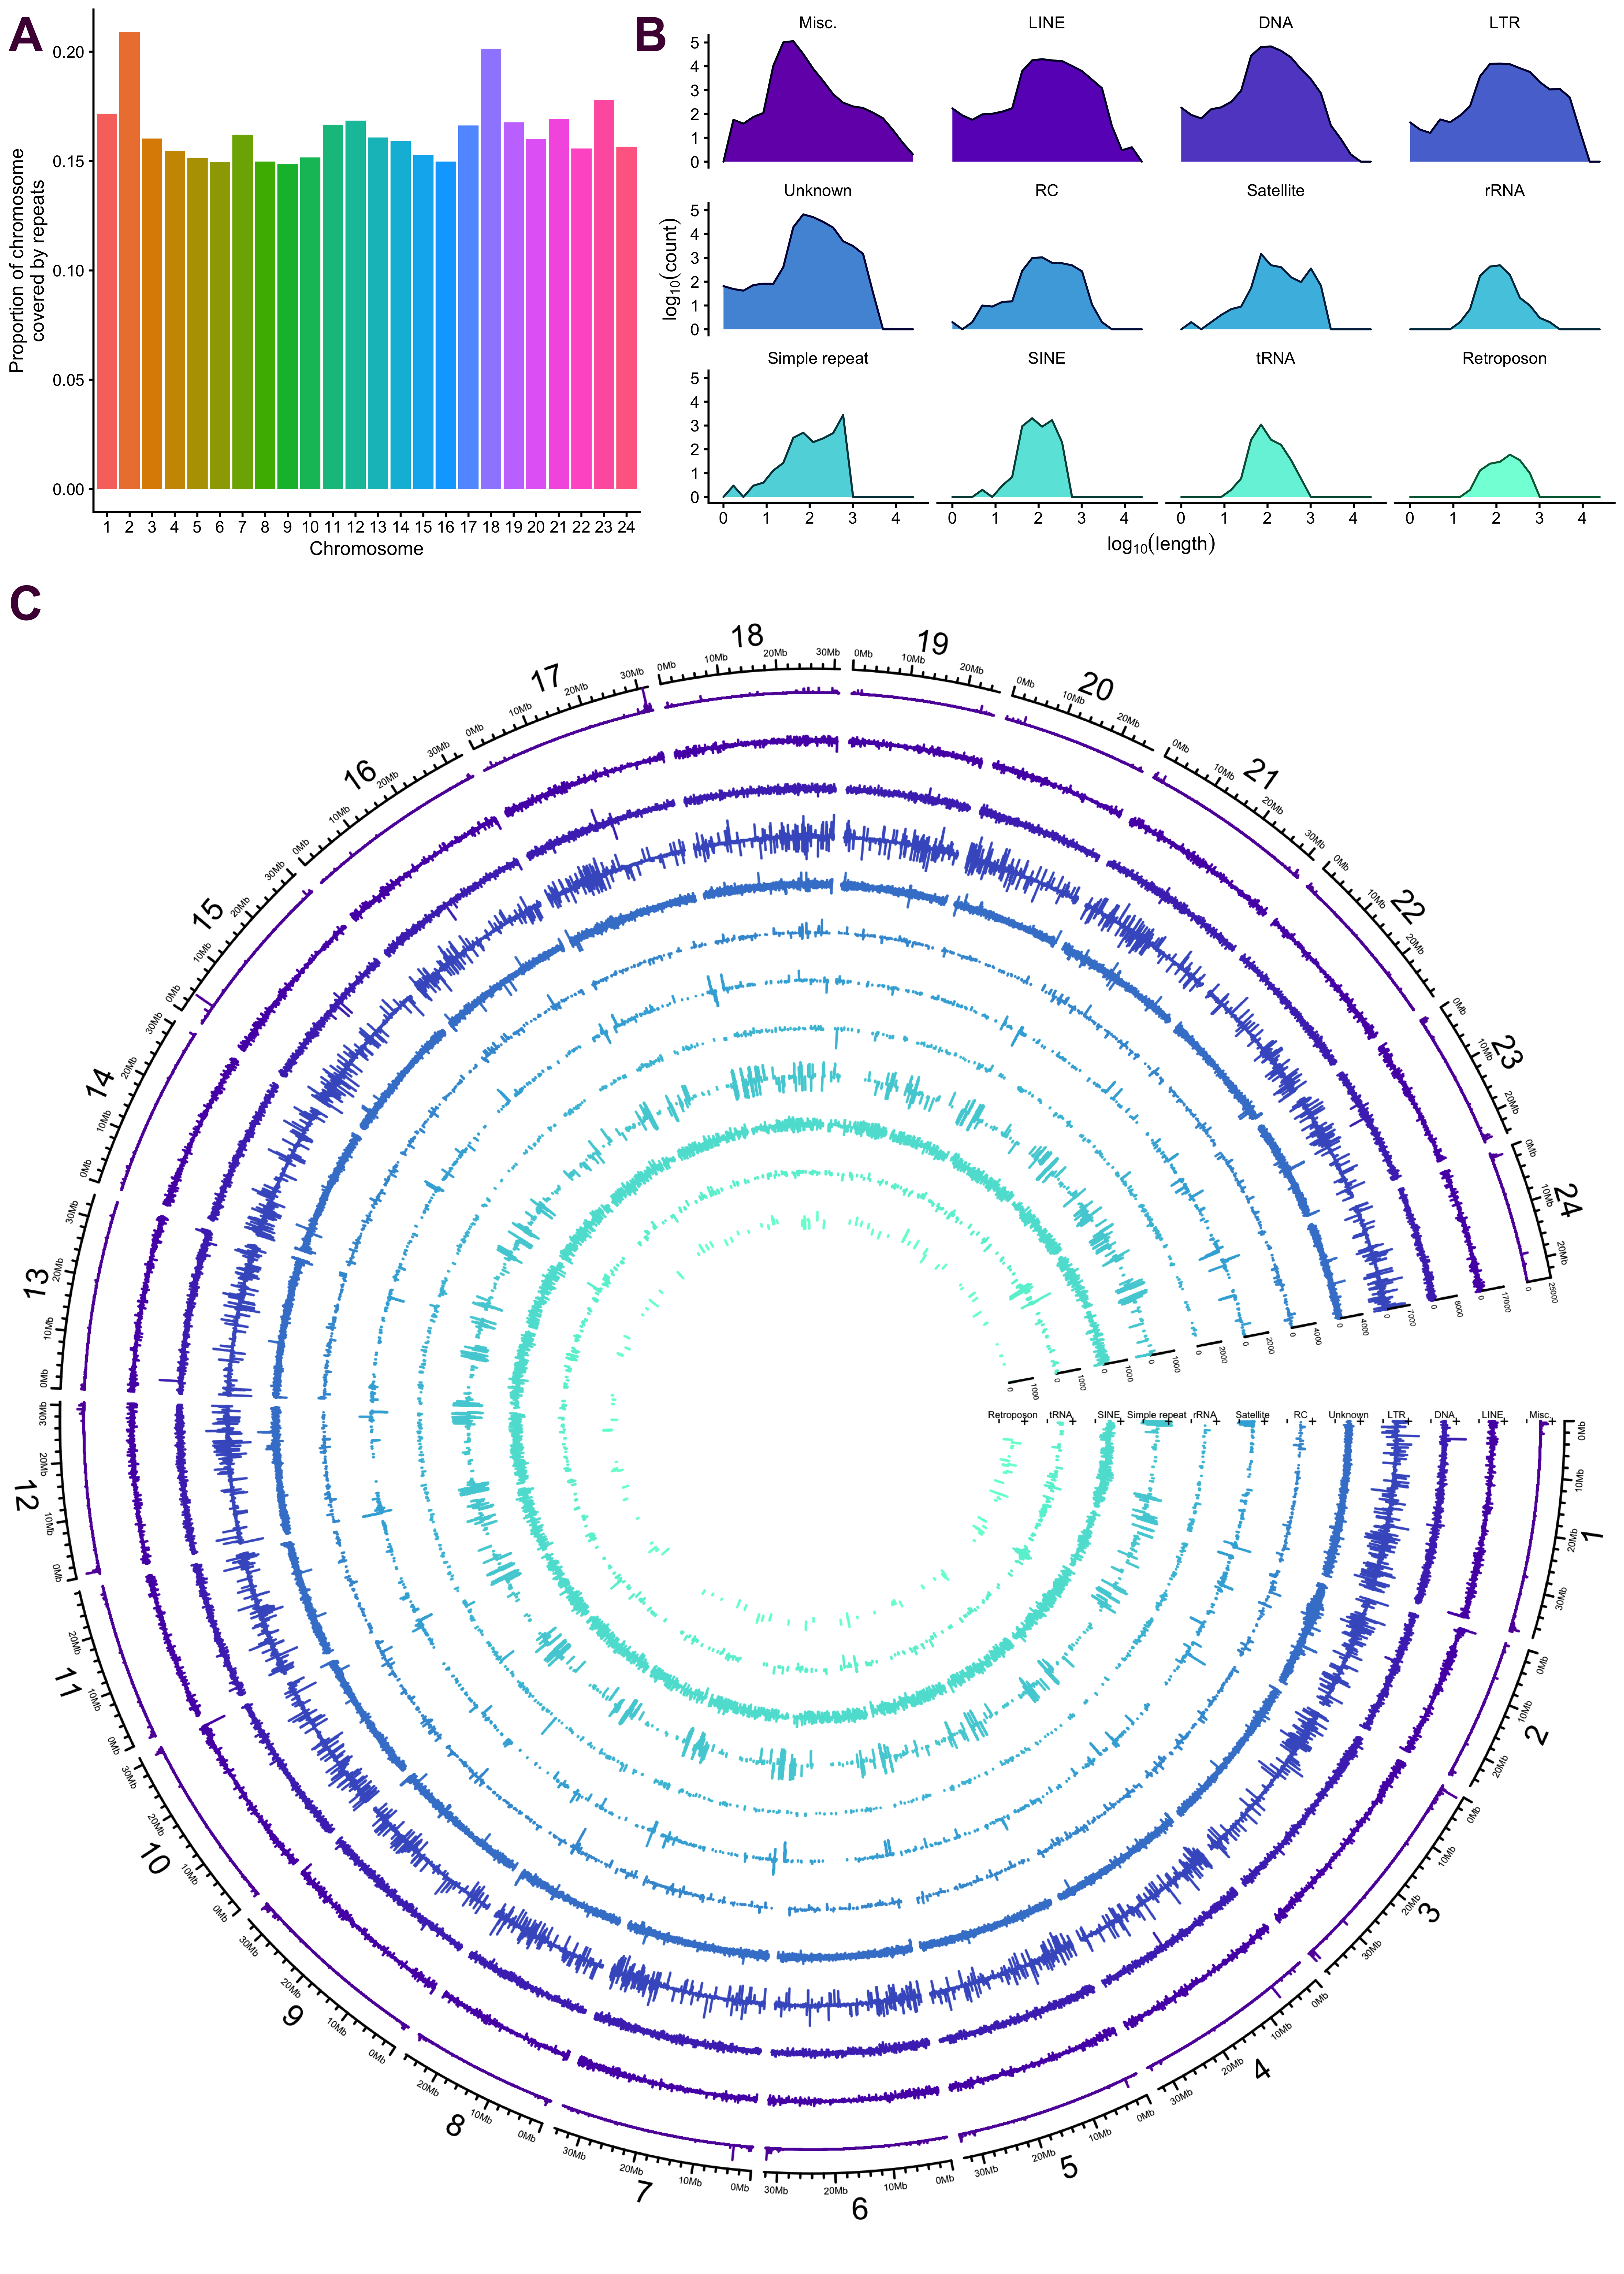
\includegraphics[width=1\linewidth]{figs/mikk_genome/20210401_hdrr_repeats_final} \caption{Repeat content in the \emph{HdrR} genome based on RepeatMasker results obtained by Jack Monahan. \textbf{A}. Proportion of repeat content per-chromosome. \textbf{B}. log10 of repeat lengths and counts per repeat class. ``Misc'' includes all repeats assigned to their own specific class, for example ``(GAG)n'' or ``(GATCCA)n''. \textbf{C}. Circos plot showing repeat length (radial axes) by locus (angular axis) and repeat class (track).}\label{fig:repeats}
\end{figure}

\hypertarget{mikksv-sec}{%
\section{Structural variation in the MIKK panel}\label{mikksv-sec}}

As an alternative to the variation pangenome approach described in Leger et al. (2022), I explored the structural variants (SVs) present in 9 of the MIKK panel lines in a reference-anchored manner, similar to many human studies. Differences in SVs between panel lines is another important class of genetic variation that could cause or contribute to significant phenotypic differences. Here we used ONT data obtained for 9 of the 12 selected lines allowing us to characterise larger SVs in the MIKK panel and to create a more extensive picture of genomic rearrangements compared to available medaka reference genomes. Adrien Leger from the Birney Group at EMBL-EBI first called structural variants using only the ONT long reads, producing a set of structural variants classified into five types: deletions (DEL), insertions (INS), translocations (TRA), duplications (DUP) and inversions (INV). I then ``polished'' the called DEL and INS variants with Illumina short reads to improve their accuracy. The polishing process filtered out 7.4\% of DEL and 12.8\% of INS variants, and adjusted the breakpoints (i.e.~start and end positions) for 75-77\% of DEL and INS variants in each sample by a mean of 23 bp for the start position, and 33 bp for the end position. This process produced a total of 143,326 filtered SVs.

The 9 ``polished'' samples contained a mean per-sample count of approximately 37K DEL variants (12\% singletons), 29.5K INS variants (14\%), 3.5K TRA variants (9\%), 2.5K DUP (7\%) and 600 INV (7\%) (\textbf{Fig. \ref{fig:SV-main}D}). DEL variants were up to 494 kb in length, with 90\% of unique DEL variants shorter than 3.8 kb. INS variants were only up to 13.8 kb in length, with 90\% of unique INS variants shorter than 2 kb. DUP and INV variants tended to be longer, with a mean length of 19 and 70.5 kb respectively (\textbf{Fig. \ref{fig:SV-main}A}). \textbf{Fig. \ref{fig:SV-main}E} shows the per-sample distribution of DEL variants across the genome. Most large DEL variants over 250 kb in length were common among the MIKK panel lines. A number of large DEL variants appear to have accumulated within the 0-10 Mb region of chromosome 2, which is enriched for repeats in the HdrR reference genome (\textbf{Fig. \ref{fig:repeats}}).

SVs were generally enriched in regions covered by repeats. While only 16\% of bases in the \emph{HdrR} reference were classified as repeats (irrespective of strand), those bases overlapped with 72\% of DEL, 63\% of DUP, 81\% of INV and 35\% of TRA variant regions. However, repeat bases only overlapped with 21\% of INS variants. We also assessed each SV's probability of being loss-of-function (pLI)(Lek et al. 2016) by calculating the logarithm of odds (LOD) for the pLI scores of all genes overlapping the variant (\textbf{Fig. \ref{fig:SV-main}B,C}). 30,357 out of 134,088 DEL, INS, DUP and INV variants overlapped at least one gene, and 9\% of those had a score greater than 10, indicating a high probability that the SV would cause a loss of function. Two INS variants on chr2 had an outlying LOD score of 57 as a result of overlapping medaka gene ENSORLG00000003411, which has a pLI score of 1 -- the highest intolerance to variants causing a loss of function. This gene is homologous with human genes \emph{SCN1A}, \emph{SCN2A} and \emph{SCN3A}, which encode sodium channels and have been associated with neuronal and sleep disorders. We did not find evidence that longer SVs tended to have a higher probability of causing a loss of function (\textbf{Fig. \ref{fig:SV-main}B}).



\begin{figure}
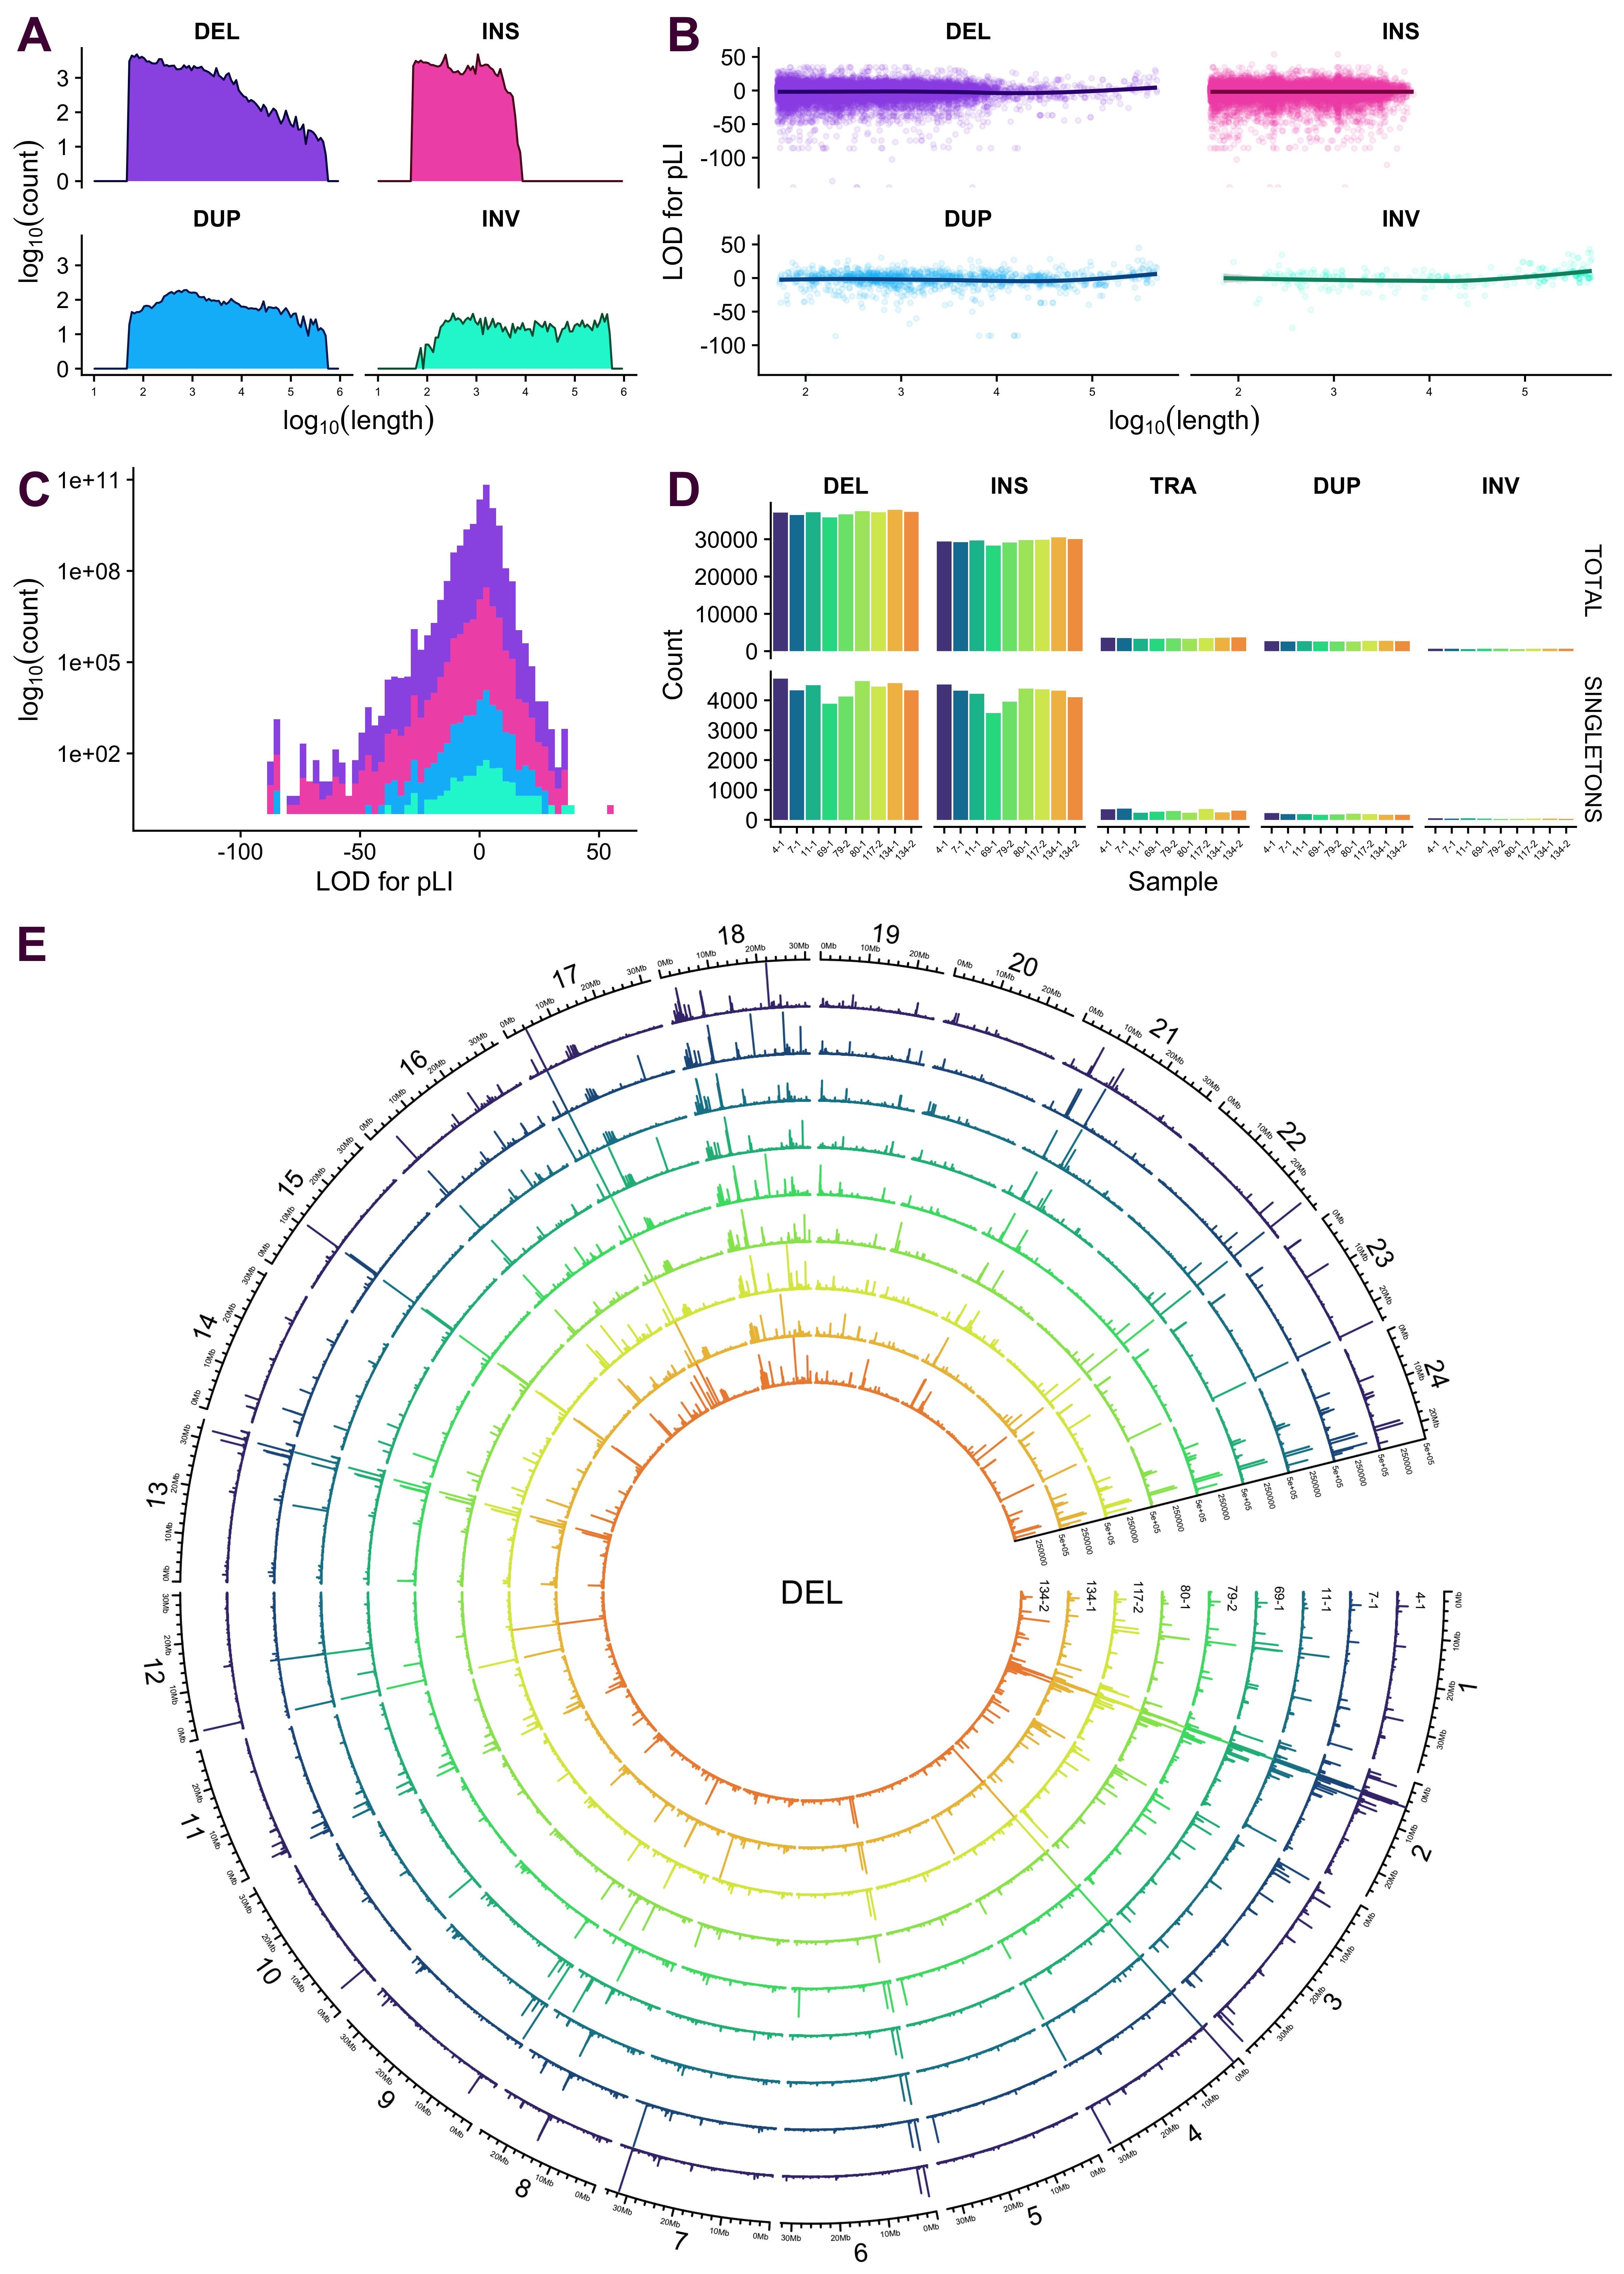
\includegraphics[width=1\linewidth]{figs/mikk_genome/20210408_sv_main} \caption{Polished SVs in 9 MIKK panel lines sequenced with ONT. DEL: deletion; INS: insertion; TRA: translocation; DUP: duplication; INV: inversion. \textbf{A}. Aggregate log10 counts and lengths of distinct SVs by type, excluding TRA. \textbf{B}. pLI LOD scores in distinct SVs by SV type. \textbf{C}. Histogram of LOD scores by SV type. \textbf{D}. Total and singleton counts of SV types per sample. \textbf{E}. Circos plot showing per-sample distribution and lengths of DEL variants across the genome.}\label{fig:SV-main}
\end{figure}

We compared these polished INS and DEL calls with the high-quality graph-based alternative paths and large-scale deletions, respectively (see section titled \emph{Novel genetic sequences and large-scale insertions and deletions in the MIKK panel} in Leger et al. (2022)). We found that 2 of the 19 regions covered by graph-based alternative paths, and 4 of the 16 regions covered by graph-based deletions, had no SVs that overlapped those regions at all, which suggests they would have been missed entirely when using a reference-anchored approach alone.

With the exception of one alternative path on chromosome 20, the alternative paths were not captured by INS variants, which only covered up to 63\% of the bases in each region, and in many cases substantially less. On the other hand, for 8 of the 16 graph-based deletions, the DEL variants covered at least 85\% of the bases in those regions. The other 8 graph-based deletions were either not at all covered by DEL variants, or only slightly. This indicates that the reference-based approach is better at detecting large-scale deletions than alternative paths (``insertions''), but still misses around half of such variants relative to the graph-based approach.

\hypertarget{conclusions}{%
\section{Conclusions}\label{conclusions}}

Taken together, these analyses show that the MIKK panel is highly homozygous, with LD characteristics that will favour high-resolution genetic mapping relative to humans. In the future, the SV analysis performed on a subset of the MIKK panel will be expanded across the entire panel, which will permit the inclusion of both large- and small-scale variants in genetic linkage studies. I proceeded to use the MIKK panel to analyse bold/shy behaviours, as I describe in Chapter \ref{MIKK-F2-chap}, with a view to carrying out an F2-cross linkage study to identify genetic variants associated with differences in the behaviours of an individual, and the extent to which they transmit those behaviours to their social companions. However, before carrying out this study, we first ran a ``pilot'' study on 5 previously-established inbred lines to validate our behavioural assay. This is the subject of the following chapter.

\hypertarget{Pilot-chap}{%
\chapter{Classification of bold/shy behaviours in 5 inbred medaka lines}\label{Pilot-chap}}

Taking advantage of the rich genetic resources offered by medaka we established an OFT to examine the performance of isogenic inbred strains for an inter-strain comparative analysis of the boldness-shyness behaviour of medaka. We used a combined open-field and novel-object assay involving assaying pairs for fish, to determine: a) whether there were consistent differences in bold-shy behaviours exhibited by 5 established inbred strains of medaka fish (\emph{iCab}, \emph{HdrR}, and \emph{HO5} from southern Japan, and \emph{Kaga} and \emph{HNI} from northern Japan); and b) whether there were consistent differences in bold-shy behaviours exhibited by a given strain (\emph{iCab}) dependent on the strain that it was partnered with. The former was intended to measure the effect of an individual's own genes on its behaviour (a direct genetic effect), and the latter to measure the effect of the genes of the focal fish's tank partner on the behaviour of the focal fish (social genetic effect). Our experimental design allowed us to assess both direct and indirect effects on behaviour simultaneously, and to infer the degree to which variation in bold-shy behaviours is attributable to the differences in an individual's own genetics, the differences in the genetics of their social companions, and stochastic variation. A schema for the experimental plan is shown in \textbf{Figure \ref{fig:behavioural-schema}}.

Schema for experimental plan. \emph{iCab}-\emph{iCab} pairings are the control condition. To explore direct genetic effects on behaviour, we compare the behaviours of test fishes from different lines, and infer that the differences between lines are caused by the differences in their genetics (direct genetic effects). To explore social genetic effects, we use the same data but turn our focus to the reference fish, and infer that the differences we observe between their behaviours are caused by the differences in their social environments, which are in turn driven by the different genetics in the test fish lines (social genetic effects). Schema for experimental plan. \emph{iCab}-\emph{iCab} pairings are the control condition. To explore direct genetic effects on behaviour, we compare the behaviours of test fishes from different lines, and infer that the differences between lines are caused by the differences in their genetics (direct genetic effects). To explore social genetic effects, we use the same data but turn our focus to the reference fish, and infer that the differences we observe between their behaviours are caused by the differences in their social environments, which are in turn driven by the different genetics in the test fish lines (social genetic effects).

\begin{figure}
\includegraphics[width=1\linewidth]{figs/pilot/experimental_schema} \caption{Schema for experimental plan. \emph{iCab}-\emph{iCab} pairings are the control condition. To explore direct genetic effects on behaviour, we compare the behaviours of test fishes from different lines, and infer that the differences between lines are caused by the differences in their genetics (direct genetic effects). To explore social genetic effects, we use the same data but turn our focus to the reference fish, and infer that the differences we observe between their behaviours are caused by the differences in their social environments, which are in turn driven by the different genetics in the test fish lines (social genetic effects).}\label{fig:behavioural-schema}
\end{figure}

{[}Wrap up the findings in one or two sentences:
We find inter-strain differences that are statistically significant
Social genetic effects that influence behaviour of a strain depending on the partner (or genetic configuration of the test pair, not sure whether this sounds ok){]}

To detect

\hypertarget{results}{%
\section{Results}\label{results}}

\hypertarget{pilot-data-collection}{%
\subsection{Data collection}\label{pilot-data-collection}}

Our behavioural assay is 20 minutes long, comprising two consecutively-run 10-minute components: a) an `open field' component, where the fishes are introduced to the test tank and left to swim around freely; and b) a `novel object' component, where a small black plastic cylinder is added to the tank at the beginning of the second 10-minute period, after which the fishes are again left to swim around freely. The assay is run on pairs of fish. Medaka is a seasonal breeder in which photoperiod has a strong effect on physiology and behaviour (L'opez-Olmeda et al. 2021). In this study we tested fish that were acclimated to summer conditions. To avoid confounding mating behaviours between males and females and associated aggressive interactions between males we used only female fish in all experiments. To increase the throughput of the assay, the test tank was divided into four quadrants with barriers, allowing us to run the assay on four pairs of fish simultaneously. Two test tanks situated side-by-side were used, allowing to run 8 concurrent assays. The experimental setup used is shown in Figure \ref{fig:assay-setup}.



\begin{figure}
\includegraphics[width=1\linewidth]{figs/pilot/setup_pic_with_frame_110} \caption{\textbf{A}: Experimental setup, with two test boxes side-by-side (denoted as ``L'' for left and ``R'' for right). Each test box contains one test tank, separated by removable barriers into quadrants, allowing for the simultaneous assay of four pairs of fish per test tank. The interior of the box is ambiently illuminated by LED lights, and a camera is suspended over the centre of each test tank to record the videos. \textbf{B}: Four pairs of fishes in a test tank with labelled quadrants (I, II, III, IV) and strains (\emph{iCab} or \emph{HdrR}). C: Paths of \emph{iCab} reference fish and \emph{HdrR} test fish from the video at panel (B) at 110 seconds.}\label{fig:assay-setup}
\end{figure}

Between 11 and 16 June 2019, I assayed a total of 307 pairs of fish, comprising the following counts for each strain pairing: 68 \emph{iCab/iCab}, 60 \emph{iCab/HdrR}, 76 \emph{iCab/HNI}, 47 \emph{iCab/Kaga}, and 56 \emph{iCab/HO5}. The locations of the lines' originating populations are shown in \textbf{Figure \ref{fig:line-locations}}. The fish from the iCab strain was denoted as the ``reference fish'', and was introduced to the test tank first. The ``test fish'' which was either another iCab fish (for the control condition), or a fish from one of the other four strains that were assayed in this experiment (\emph{HdrR}, \emph{HNI}, \emph{Kaga}, \emph{HO5}). The order in which the strains were assayed across the six days was randomly determined prior to the collection of the data. The test tanks were also rinsed between runs to remove any substances released by subjects during previous runs that could influence the behaviour of the subjects that followed.

Image adapted from (Spivakov et al. 2014), showing the locations of the originating populations of the 5 inbred medaka lines used in this study. Image adapted from (Spivakov et al. 2014), showing the locations of the originating populations of the 5 inbred medaka lines used in this study.

\begin{figure}
\includegraphics[width=1\linewidth]{figs/pilot/line_locations} \caption{Image adapted from (Spivakov et al. 2014), showing the locations of the originating populations of the 5 inbred medaka lines used in this study.}\label{fig:line-locations}
\end{figure}

\hypertarget{tracking}{%
\subsection{Tracking}\label{tracking}}

We split the videos by quadrant and assay component, and tracked the movement of the fishes with the open-access software package \emph{idtrackerai} (Romero-Ferrero et al. 2019). Each individual fish was tracked across at least 85\% of frames in each video, with 78\% of videos tracked for over 99\% of frames. The failure to track both fishes across all frames was usually caused by instances where a fish was situated behind the novel object or quadrant divider, rendering it invisible to the camera. A random selection of 20 videos was reviewed to search for instances of mislabeled fishes due to software errors. We found none, which is consistent with the reliability of the software as reported by its authors. We therefore concluded that such instances would be absent or very rare and thus negligible.

To identify which fish was the reference or test fish, we could generally distinguish between the strains based on their colour, as \emph{iCab} pigmentation is light-brown, \emph{HO5} are light-brown with an orange hue, \emph{HdrR} females are white, and \emph{HNI} and \emph{Kaga} are grey. Where the reference fish was indistinguishable in colour from the test fish, we identified the fish that was introduced to the test tank first, and followed it by eye through to the first frame of the assay. In cases of \emph{iCab}-\emph{iCab} pairings, we randomly assigned the individuals to either the ``reference'' or ``test'' fish.

We then used the coordinates of the fishes in each frame to calculate the distance and angle travelled by each fish between a fixed time interval, for example every 0.05 seconds. Distance was calculated between points B → C, and angle was calculated between points A → B → C. We used these distance and angle variables to train a HMM with the \emph{hmmlearn} Python package (\emph{Hmmlearn/Hmmlearn} {[}2014{]} 2022) in order to classify the movements as discrete behaviours or ``modes of movement''.

\hypertarget{effect-of-covariates}{%
\subsection{Effect of covariates}\label{effect-of-covariates}}

We examined the effects of several covariates, including date of assay, time of assay, tank quadrant, and tank side. To achieve this, we calculated the mean speed of individuals in \emph{iCab}-\emph{iCab} pairings (\(N\) = 136) over the course of the entire 20-minute video (including both open field and novel object assays), and ran a multi-way ANOVA with all covariates (\textbf{Figure \ref{fig:covariate-effects}}). We found significant differences for date of assay and and tank quadrant (p = 0.0139 and 0.0108), but not for time of assay or tank side. This may have been driven by a difference in the way the assay was performed on the first day of the experiment (11 June 2019), where we used a thick fabric sheet to cover the front of the box rather than the wooden doors shown in \textbf{Figure \ref{fig:assay-setup}}, as they were only installed the following day. The greater level of external light and sound permeating through the fabric may have caused the fishes to exhibit slower movement on that first day, and when the data from that day is excluded, the p-values for date of assay and tank quadrant increase to 0.0477 and 0.0469 respectively.



\begin{figure}
\includegraphics[width=1\linewidth]{figs/pilot/covariate_effects_no-split-by-assay} \caption{Effect of covariates on mean speed of iCab individuals when paired with another iCab over the course of the full video (including both open field and novel object assays). \emph{P}-values were calculated from a multi-way ANOVA with all four covariates included as terms, and adjusted for false discovery rate.}\label{fig:covariate-effects}
\end{figure}

\hypertarget{pilot-hmm-params}{%
\subsection{Choice of time interval and number of HMM states}\label{pilot-hmm-params}}

HMMs are well-suited for classifying the hidden states that generate stochastic, sequential observations. To determine the optimal parameters for the HMM's classification of behaviours, we sought to reduce overfitting (which tends to favour using a lower number of HMM states) while maximising the ability to distinguish between strains based on the relative time they spent in each HMM state (which tends to favour a higher number of HMM states). We additionally considered the time interval between which the distance and angle of travel was measured.

\textbf{Figure \ref{fig:compare-params}} sets out the comparison of HMM parameters on two measures designed to quantify, respectively, the level of overfitting (`mean concordance between cross-validated HMM states'), and the quantification of differences between strains ('summed Kruskal-Wallis statistic comparing frequency of time spent in each HMM state across medaka strains) (Methods).



\begin{figure}
\includegraphics[width=1\linewidth]{figs/pilot/compare_params} \caption{Comparison between HMM parameters. Horizontal axis: Mean concordance between states assigned by HMMs through a 2-fold cross-validation process. Vertical axis: Kruskal-Wallis statistic comparing strains based on the proportion of time spent in each HMM state, summed across all states. Size of points correspond to the interval, in seconds, between which the distance and angle of travel was calculated (Methods).}\label{fig:compare-params}
\end{figure}

Based on these results and a visualisation of the polar plots for each combination of state number and time interval, we excluded combinations with 15 or more states due to an asymmetry across states that would create difficulties for interpreting their biological meaning (Supplementary material). For the downstream analysis we selected the combination of 14 states with a 0.08-second interval between time points, because out of the remaining combinations it appeared to optimally balance the level of overfitting and detection of differences between strains.

The distances and angles of travel for the 14 states are shown in Figure 4, generated from 10,000 randomly-selected data points (i.e.~movements). Each point represents the radial distance in log10(pixels) that a fish travelled from its previous location (B → C), and the polar angle travelled from A → B → C, where A → B is always aligned vertically along the 0-180° axis. For example, a point at 45° far from the pole represents a fast, forward movement to the right, and a point at 260° close to the pole represents a slow, backward movement to the left.



\begin{figure}
\includegraphics[width=1\linewidth]{figs/pilot/polar_all_dge} \caption{Classification of movements by the 14-state HMM, based on distance (in log10(pixels)) and angle of travel between a time interval of 0.08 seconds from points B → C for distance, and points A → B → C for angle. Each point represents the distance and angle at point C, and A → B is aligned vertically along the 0-180° radial axis. The figure shows an illustrative 10,000 data points (movements), randomly selected from the full dataset. States are sorted in ascending order by mean distance.}\label{fig:pilot-polar}
\end{figure}

We next sought to determine whether there was a difference in the proportion of time spent in each state between the 5 inbred strains (implying the presence of direct genetic effects), and between the \emph{iCab} reference fishes depending on the inbred strains of their tank partner (implying the presence of social genetic effects).

\hypertarget{direct-and-social-genetic-effects-on-boldshy-behaviour}{%
\subsection{Direct and social genetic effects on bold/shy behaviour}\label{direct-and-social-genetic-effects-on-boldshy-behaviour}}

\hypertarget{direct-genetic-effects}{%
\subsubsection{Direct genetic effects}\label{direct-genetic-effects}}

To determine whether the test fish strains differed in the proportions of time they spent in each state, we ran separate multi-way ANOVAs for each combination of assay component (open field or novel object) and state (states 1 to 14):

\[
frequency_{assay component,state} = \beta_{1}(test fish strain) + \beta_{2}(date) + \beta_{3}(time) + \beta_{4}(quadrant) + \beta_{5}(tank side)
\]

The proportion of time each individual spent within a state was first inverse-normalised within each combination of assay and state, and the date of assay, time of assay, tank quadrant, and tank side were included as covariates. P-values were then adjusted for the False Discovery Rate (\textbf{FDR}).

The states that showed a significant difference are set out in \textbf{Table \ref{tab:pilot-dge-tbl}}. The test fish strains differed significantly in the proportion of time spent in a given state (p \textless{} 0.05, FDR-adjusted) for 11 out of 14 states in the open field assay (4.45x10-24 \textless{} p \textless{} 1.06x10-2), and 7 out of 14 states for the novel object assay (5.53x10-16 \textless{} p \textless{} 4.2x10-3), with the strain of the test fish explaining up to \textasciitilde28\% of the variance in the proportion of time spent in a given state. For some states, there was also a significant difference between quadrants, date of assay, and tank side (open field: 1.03e-09 \textless{} p \textless{} 1.18x10-2; novel object: 1.75x10-8 \textless{} p \textless{} 4.9x10-2). Full tables for all states and variables are provided in the Supplementary Material.

\begin{table}

\caption{\label{tab:pilot-dge-tbl}Significant differences in the proportion of time spent in each HMM state across test fish strains for the open field and novel object assay components.}
\centering
\begin{tabular}[t]{llll}
\toprule
Assay & State & Variance explained (\%) & p-value (FDR-adjusted)\\
\midrule
open field & 1 & 26.62 & 3.60e-22\\
open field & 2 & 21.94 & 6.18e-18\\
open field & 3 & 28.21 & 4.45e-24\\
open field & 4 & 17.73 & 2.12e-15\\
open field & 5 & 7.48 & 2.78e-05\\
\addlinespace
open field & 6 & 5.60 & 2.48e-04\\
open field & 7 & 5.46 & 3.11e-04\\
open field & 8 & 5.79 & 1.08e-04\\
open field & 9 & 7.36 & 8.96e-06\\
open field & 10 & 3.78 & 1.06e-02\\
\addlinespace
open field & 13 & 4.66 & 3.42e-03\\
novel object & 1 & 17.19 & 7.28e-14\\
novel object & 2 & 14.28 & 2.92e-11\\
novel object & 3 & 19.30 & 5.53e-16\\
novel object & 4 & 13.12 & 1.26e-10\\
\addlinespace
novel object & 6 & 4.12 & 4.20e-03\\
novel object & 7 & 8.93 & 1.84e-06\\
novel object & 9 & 10.68 & 9.87e-08\\
\bottomrule
\end{tabular}
\end{table}

\textbf{Figure \ref{fig:pilot-dge-time}} depicts the time dependence of HMM states over the course of the video, and the regions of the test tank that were most frequently occupied by the different strains. Figures A and H show the HMM states with panels coloured red to indicate the states that were found to significantly differ between test fish strains. \textbf{Figures \ref{fig:pilot-dge-time}B} and \textbf{E} show how each individual test fish, grouped by inbred strain, moved through HMM states throughout the course of the video, with each tile coloured by the state most frequently-occupied by the individual within 2-second intervals. Figures \textbf{\ref{fig:pilot-dge-time}C} and \textbf{F} show the same data, recalculated as densities within each strain, with only the states that showed significant differences between strains in colour, and the remaining states consolidated and coloured grey. There is an especially clear difference between strains in the proportions of time spent in the slowest-moving states (i.e.~states 1 to 3) at the beginning of each assay component, with an increase across all strains in the novel object assay, likely as a consequence of having less room to move, as well as the fear response that the novel object was designed to elicit. The differences are clearest when comparing the southern Japanese medaka strains (\emph{iCab}, \emph{HdrR}, and \emph{HO5}) against the northern Japanese strains (\emph{Kaga} and \emph{HNI}). In addition, we note that \emph{Kaga} tends to spend more time in the fast- and forward-moving state 13 at the beginning of the assay than at other times, which suggests that for that strain, such movements may be the manifestation of a stress response. \textbf{Figures \ref{fig:pilot-dge-time}D} and \textbf{G} show, as densities, the regions of the tank that were most frequently occupied by each strain. Although the northern Japanese strains \emph{Kaga} and \emph{HNI} were similarly fast-moving relative to the southern Japanese strains, in the open field assay component they appear to favour different regions of the tank -- where \emph{HNI} occupied the central regions of the tank with more frequency, \emph{Kaga} tended to prefer swimming along the boundaries of the tank.



\begin{figure}
\includegraphics[width=1\linewidth]{figs/pilot/0.08_14_dge} \caption{Differences between test fish strains in the HMM states they occupied during the open field (top) and novel object (bottom) assay components. \textbf{A and H}: 14 HMM states with panels coloured red to indicate significant differences between test fish strains in the proportion of time spent in those states during the separate assay components. \textbf{B and E}: Transitions between HMM states across time for each individual test fish, grouped by strain. Tiles are coloured by the state most frequently occupied by each fish within 2-second intervals. \textbf{C and F}: Densities within each strain for the occupation of states that significantly differed between strains (colour), with other states consolidated (grey). \textbf{D and G}: Densities of the test tank locations occupied by each strain, calculated within 900 grid points (30x30).}\label{fig:pilot-dge-time}
\end{figure}

\hypertarget{pilot-sge}{%
\subsubsection{Social genetic effects}\label{pilot-sge}}

To determine whether the \emph{iCab} reference fishes altered their behaviour depending on the inbred strain of their tank partner, we carried out the same analysis and model as above using only data from the \emph{iCab} reference fishes. The states that showed a significant difference are set out in \textbf{Table \ref{tab:pilot-sge-tbl}}. The \emph{iCab} reference fishes differed significantly in the proportion of time they spent in a given state depending on the strain of their tank partner (\(p\) \textless{} 0.05, FDR-adjusted) for 5 out of 14 states in the open field assay (2.04x10-6 \textless{} \(p\) \textless{} 2.11x10-2), and 7 out of 14 states for the novel object assay (4.76x10-7 \textless{} \(p\) \textless{} 4.06x10-2). The strain of the tank partner explained up to \textasciitilde9\% of the variance in the proportion of time the \emph{iCab} reference spent in a given state. Full tables for all states and variables are provided in the Supplementary Material.

\begin{table}

\caption{\label{tab:pilot-sge-tbl}Significant differences in the proportion of time spent in each HMM state by iCab reference fishes depending on the strain of their tank partner during the open field and novel object assay components.}
\centering
\begin{tabular}[t]{llll}
\toprule
Assay & State & Variance explained (\%) & p-value (FDR-adjusted)\\
\midrule
open field & 1 & 8.52 & 5.88e-06\\
open field & 2 & 9.09 & 2.04e-06\\
open field & 3 & 7.97 & 1.77e-05\\
open field & 5 & 3.92 & 4.29e-03\\
open field & 12 & 2.97 & 2.11e-02\\
\addlinespace
novel object & 1 & 7.94 & 8.73e-06\\
novel object & 2 & 9.38 & 4.76e-07\\
novel object & 3 & 8.73 & 1.58e-06\\
novel object & 6 & 4.76 & 1.23e-03\\
novel object & 8 & 2.80 & 4.06e-02\\
\addlinespace
novel object & 10 & 3.81 & 8.43e-03\\
\bottomrule
\end{tabular}
\end{table}

We observe that the proportions of time the \emph{iCab} reference fishes spent in different states do differ based on the strains of their tank partner, and that their behavioural patterns tend to reflect those of the test fish strains they are paired with (\textbf{Figure \ref{fig:pilot-sge-time}}). Thus, the \emph{iCab} reference fishes spend less time in the slower-moving states when in the presence of the faster-moving northern Japanese strains \emph{Kaga} and \emph{HNI}, which in turn shows that the test fishes are transmitting their behaviours to some degree to their \emph{iCab} tank partners.The differences in the behaviours of \emph{iCab} reference fishes based on the strain of their tank partners are not as large as those between the test fish strains. However, unlike what was observed with the test fishes, here there is a greater number of states that show significant differences during the novel object component of the assay compared to the open field component. This suggests that when movement is restricted, or when in the presence of a potential threat, the behaviour of the test fish tank partner has more of an influence on the \emph{iCab} reference fish's behaviour than otherwise.



\begin{figure}
\includegraphics[width=1\linewidth]{figs/pilot/0.08_14_sge} \caption{Differences between HMM states occupied by the reference fish when paired with different test fish strains during the open field (top) and novel object (bottom) assay components. \textbf{A and H}: 14 HMM states with panels coloured red to indicate significant differences between the reference fishes under different strain-pairings in the proportion of time spent in those states during the separate assay components. The HMM states are the same as those in \textbf{Figure \ref{fig:pilot-dge-time}}, but coloured with a different palette. \textbf{B and E}: Transitions between HMM states across time for each individual \emph{iCab} reference fish, grouped by the strain of its tank partner. Tiles are coloured by the state most frequently occupied by each fish within 2-second intervals. \textbf{C and F}: Densities within each strain-pairing for the occupation of states that significantly differed between strain-pairings (colour), with other states consolidated (grey). \textbf{D and G}: Densities of the test tank locations occupied by the iCab reference fishes when paired with different strain, calculated within 900 grid points (30x30).}\label{fig:pilot-sge-time}
\end{figure}

Finally, to develop a metric to quantify the degree to which the \emph{iCab} reference fishes' behaviour is influenced by the strain of its tank partner, we calculated the proportions of time that the pairs of fish spent simultaneously occupying the same HMM state. \textbf{Figure \ref{fig:pilot-cooc-heat}} shows that when paired with the slowest-moving \emph{HdrR} strain, the \emph{iCab} reference fishes spent more time co-occupying the slow- and forward-moving state 2, whereas they tended to co-occupy the fast- and forward-moving state 11 when paired with the faster-moving northern \emph{Kaga} and \emph{HNI} strains. When paired with another \emph{iCab}, they preferred to co-occupy the slow-moving and pan-directional state 4. For each combination of assay component and state, we then ran a Kruskal-Wallis test to determine whether there were differences in the frequencies of state co-occupancy under different strain pairings (\(p\) \textless{} 0.05, FDR-adjusted), and found significant differences for states 1 to 6 for the open field component (1.1x10-8 \textless{} \(p\) \textless{} 4.1x10-2), and states 1 to 4 and 7 for the novel object component (1.6x10-6 \textless{} \(p\) \textless{} 2.5x10-2). The heatmaps show that \emph{iCab} tends to co-occupy state 4 at the highest frequency when paired with another \emph{iCab}, which suggests that this pan-directional, slow-moving state is a more comfortable or natural state for \emph{iCab} to occupy, particularly when under stress.



\begin{figure}
\includegraphics[width=1\linewidth]{figs/pilot/0.08_14_cooc_heatmap} \caption{Frequency of HMM state co-occupancy between pairs of fish, calculated across all all videos per strain-pairing.}\label{fig:pilot-cooc-heat}
\end{figure}

\hypertarget{discussion}{%
\section{Discussion}\label{discussion}}

In this chapter have described an assay for measuring bold-shy behaviours in medaka fish that can reliably detect differences: (a) between individuals from different inbred strains -- allowing for the quantification of direct genetic effects on behaviour; and (b) between the behaviour of individuals when paired with tank partners from a different strain -- allowing for the quantification of social genetic effects on behaviour.

I found that behaviours exhibited during the assay show minimal variance across the covariates of date of assay, time of assay, tank quadrant, and tank side. This creates confidence that the genetic effects that we observed -- both direct and indirect -- are not unduly affected by these variables.

I have shown that a Hidden Markov Model (HMM) allows an adequate classification of movements based on the direction and angle of travel within set time intervals. The HMM method has previously been used to classify maternal behaviour patterns in mice (Carola, Mirabeau, and Gross 2011), and I have extended the application here to bold-shy behaviours in medaka fish. In principle, this method can be expanded to include additional behavioural features such as proximity to the wall or other objects, inwards/outwards orientation, proximity to the tank partner, and other metrics related to leader-follower dynamics, a possibility that will be tested in future studies.

The HMM classification of behaviours also facilitated the ranking of behaviours by speed and angle of movement, which may be further interpreted in terms of biology and adaptation styles. However, even though the HMM classifies the slowest-moving states as separate modes of movement, one should be cautious when attributing biological meaning to their differences, because even when a fish is almost completely still, the fish object's centroid (upon which the variables of distance and angle of travel are calculated) will tend to move by one or several pixels through minor changes in the segmentation of the object, and are thus subject to greater noise than the faster-moving states.

I have found that inbred strains of medaka fish can be distinguished by the proportion of time they spend in certain states. The slowest states, capturing no or minimal movement, were the states that most clearly separated the strains, and these differences appeared most clearly at the beginning of the open field and novel object assays. This suggests that for southern Japanese strains such as \emph{iCab}, \emph{HdrR}, and \emph{HO5}, the ``freeze'' reflex is caused by anxiety, which eventually dissipates over time indicating habituation. Similar observations showing initial anxiety as shown by freezing behaviour and subsequent habituation have been made in other studies using open field assays with \emph{iCab} fish (Lucon-Xiccato et al. 2022).

On the other hand, the northern Japanese strains \emph{Kaga} and \emph{HNI} spent little time in the slow-moving states at the beginning of the video, which indicates either that their habituation sets in earlier, or that their stress and anxiety is expressed to a lesser degree as freezing behaviour. The former appears to be more likely for \emph{Kaga}, as in the open field assay, it spends more time in the faster-moving states at the beginning of the video and then slows down thereafter, which suggests that its higher level of movement may be induced by stress. It is interesting then that once the novel object is introduced, \emph{Kaga} tends to move slowly like the other strains. Obviously introduction to a novel environment and exposure to a potentially dangerous object elicits different behavioural patterns in this strain. Taken together with the overt thigmotaxis behaviour (i.e.~moving along the sides of the tank during the open field assay component) relative to other strains, its behaviour may suggest an ``escape-seeking'' response. It will be interesting to carry out further experiments to determine under which fear-inducing conditions \emph{Kaga} reacts with this more frantic style of movement rather than the freeze response that it displays in the novel object component in common with the other strains, and to explore its physiological basis.

With respect to social genetic effects, we have found that a fish's behaviour is affected by the differential behaviour of its tank partner, although the effect is less powerful than the direct genetic effect on a fish's own biology. These social genetic effects are detectable when observing the proportions of time the reference fishes spend in certain states over the course of the video, and can be quantified by measuring the frequency of state co-occupancy with their tank partners.

It is also interesting to find that \emph{iCab} prefers to co-occupy the slow, pan-directional state 4 when paired with another individual from the same strain. As the strains are raised exclusively in the company of individuals from the same strain, that type of behaviour may represent a more comfortable -- yet still cautious -- mode of movement, or a type of mimicry that tends to occur when in the company of individuals that are more genetically or socially familiar.

In this study we only used one strain as the reference fish, but future experiments can expand on this analysis by using different strains as the reference, thereby exploring how a strain's genetics influence the degree of their behavioural plasticity, and how the distinct behaviours of strains may interact in intriguing ways.

In summary we show that the OFT experimental setup in combination with the HMM analysis can reliably detect both direct and social genetic effects. This creates the opportunity to carry out a similar study on a larger panel of inbred strains, such as the MIKK panel (Fitzgerald et al. 2022), with a view to identifying the genetic variants associated with not only these differences in behaviour, but also the differences in the degree to which an individual transmits their behaviour onto their social companions. This in turn will shed light on longstanding biological questions concerning the direct and indirect influences on behaviour, their physiological bases, and their adaptive purposes. This is the subject of the following chapter.

\hypertarget{Somite-chap}{%
\chapter{Genetic loci associated with somite development periodicity}\label{Somite-chap}}

\chaptermark{Somite development periodicity}

\hypertarget{section}{%
\section[\definecolor{chapter_col}{HTML}{3B0023}\textcolor{chapter_col}{Background}]{\texorpdfstring{\definecolor{chapter_col}{HTML}{3B0023}\textcolor{chapter_col}{Background}\footnote{This Chapter describes a project carried out in collaboration with Ali Seleit and Alexander Aulehla from the Aulehla Group at EMBL Heidelberg. Drs Seleit and Aulehla performed the experiments and gathered the data; my role was to carry out the bioinformatics involved in mapping the genetic variants associated with the phenotypes of interest.}}{}}\label{section}}

\par

\noindent

\rule{\textwidth}{0.4pt}

During the development of an embryo, somites are the earliest primitive segmental structures that form from presomitic mesoderm cells (\textbf{PSM}) (Kim et al. 2011). They later differentiate into vertebrae, ribs, and skeletal muscles, thereby establishing the body's anterior-posterior axis. \textbf{Figure \ref{fig:mouse-embryo}} depicts a number of formed somites in a 9.5-day-old mouse embryo.

Image of a mouse embryo at day 9.5 from Gridley (2006), showing somites in darker colours. Image of a mouse embryo at day 9.5 from Gridley (2006), showing somites in darker colours.

\begin{wrapfigure}{L}{0.4\textwidth}
\includegraphics[width=1\linewidth]{figs/somites/mouse_embryo_gridley} \caption{Image of a mouse embryo at day 9.5 from Gridley (2006), showing somites in darker colours.}\label{fig:mouse-embryo}
\end{wrapfigure}

Somite formation occurs rhythmically and sequentially, with the time between the formation of each pair of somites referred to as the ``period''. The period of somite formation varies greatly between species: \textasciitilde30 minutes for zebrafish, 90 minutes for chickens, 2-3 hours for mice, and 5-6 hours for humans (Hubaud and Pourqui'e 2014; Matsuda et al. 2020). \textbf{Figure \ref{fig:somite-seg-ali}} shows the a series of time-stamped images of somite segmentation in medaka fish, generated by Ali Seleit.

Time-stamped images of somite segmentation in medaka, generated by Ali Seleit. Time-stamped images of somite segmentation in medaka, generated by Ali Seleit.

\begin{figure}
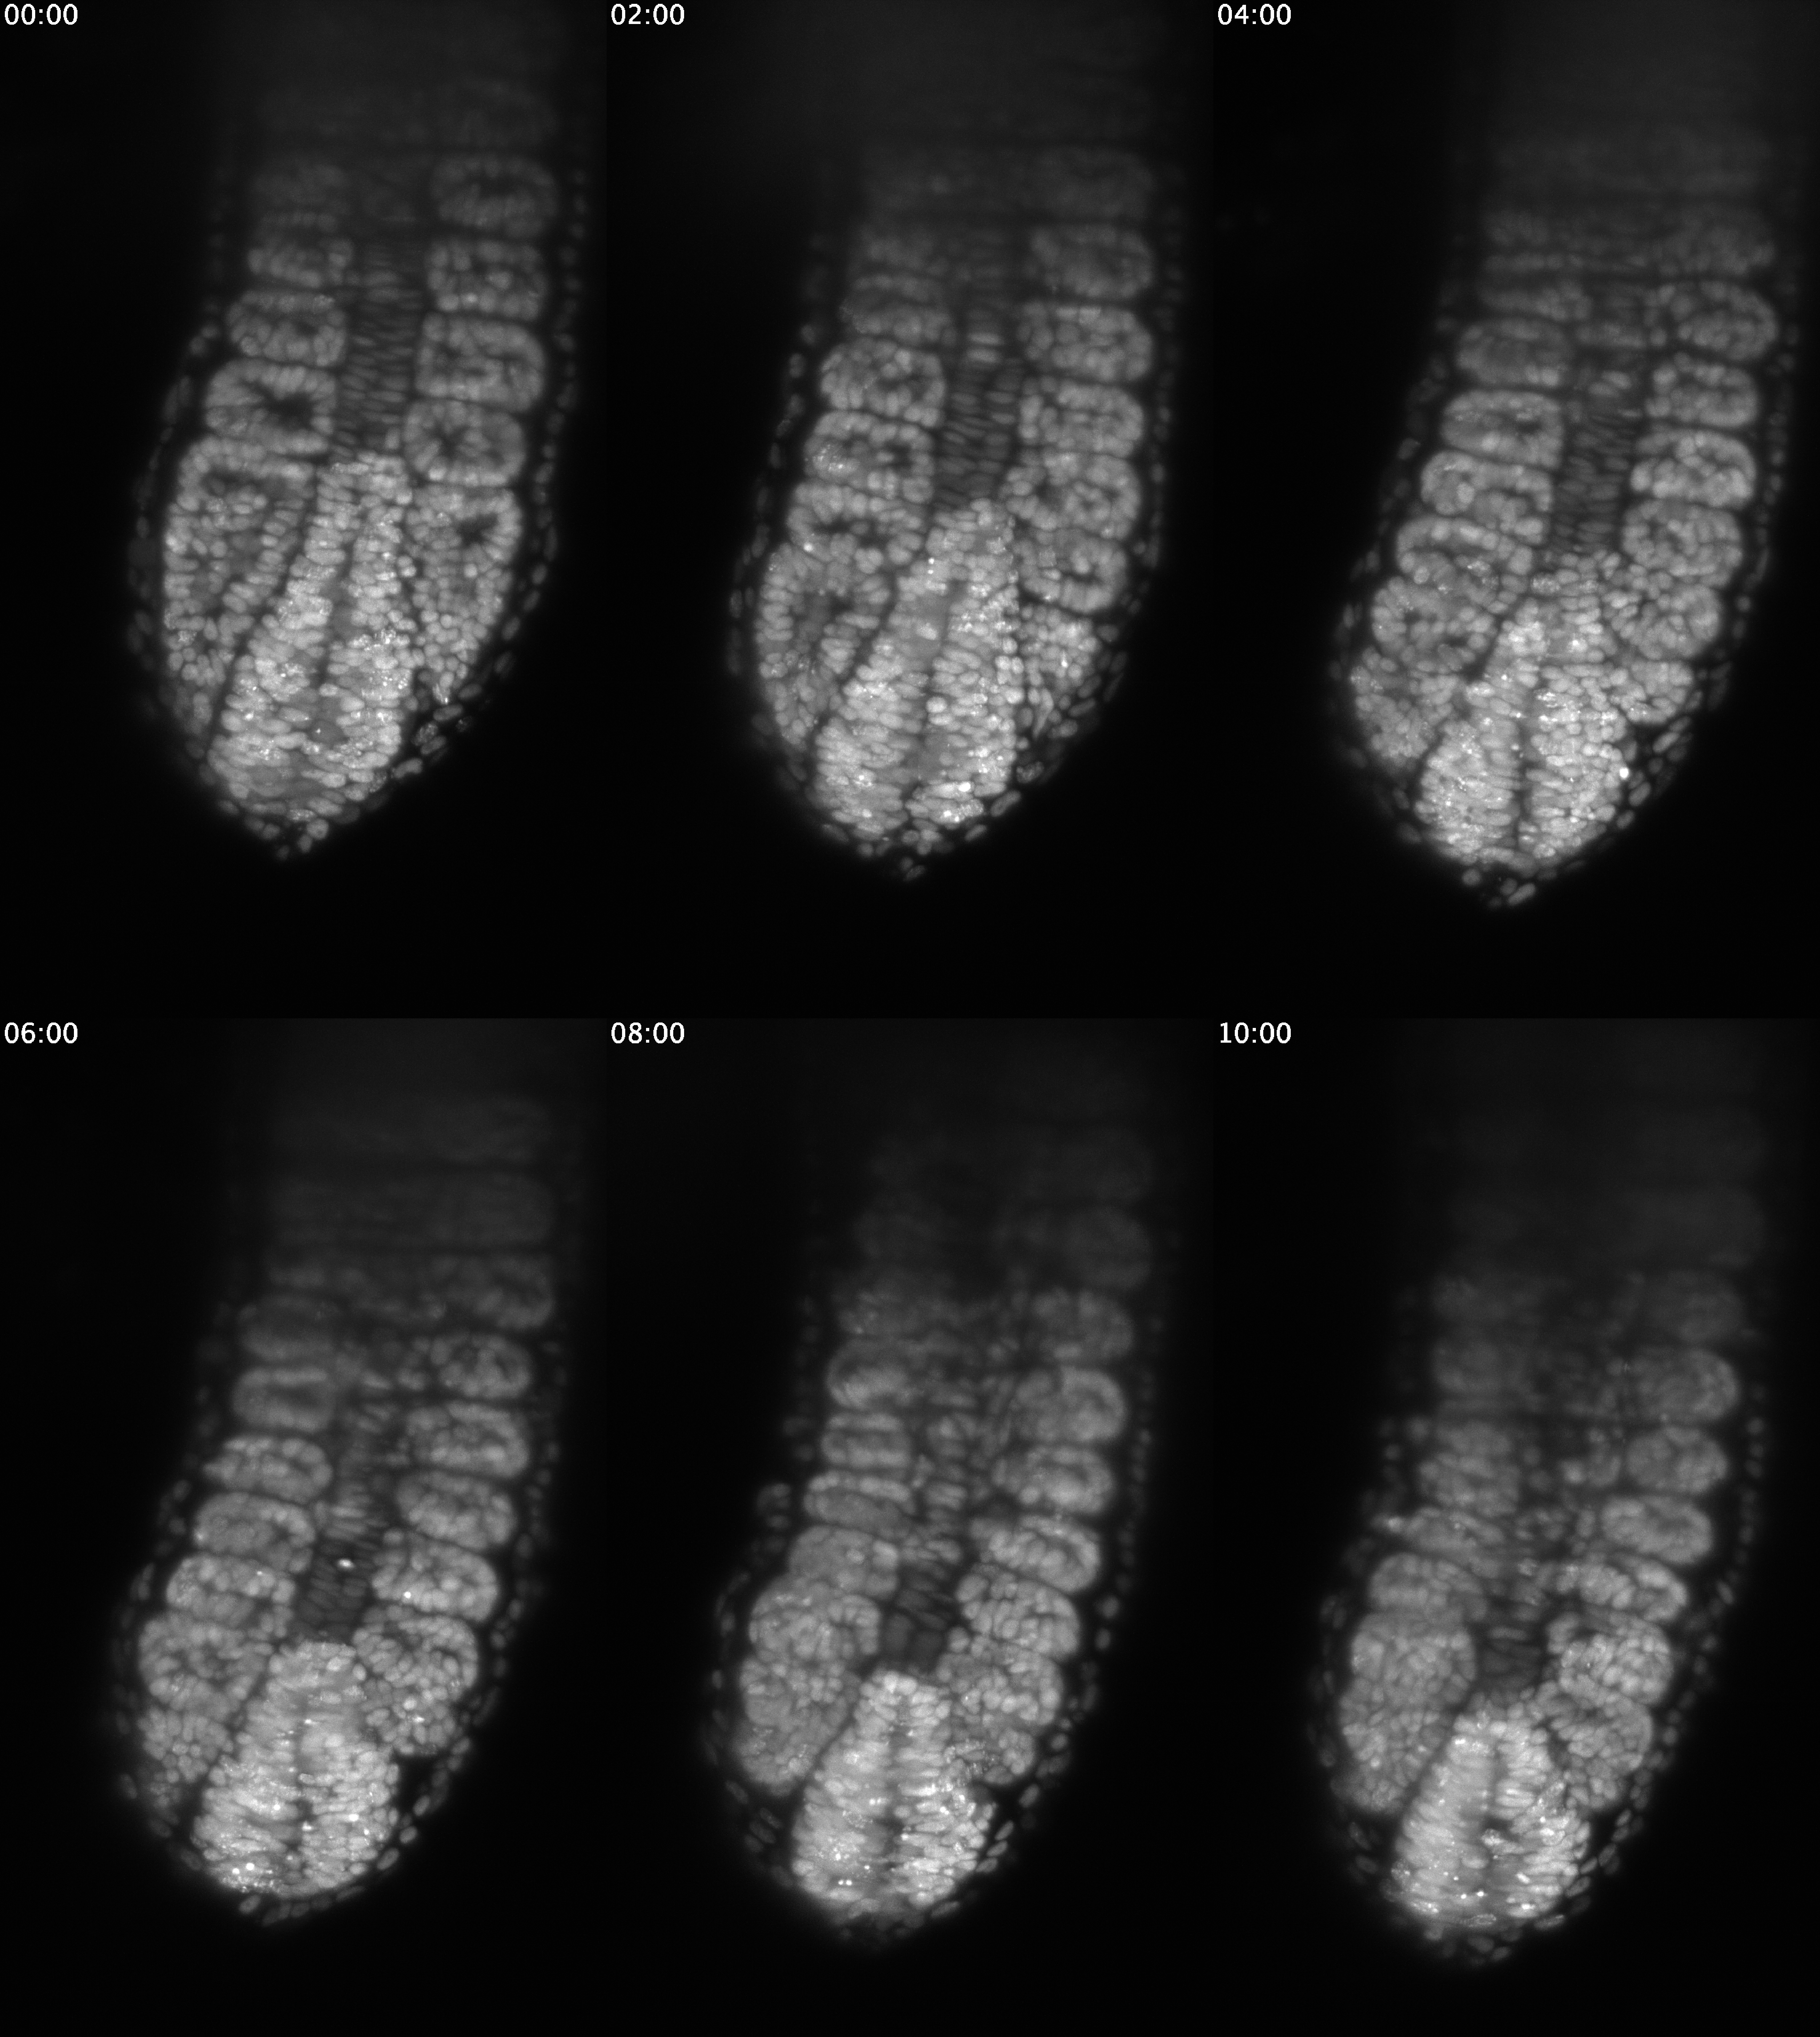
\includegraphics[width=1\linewidth]{figs/somites/ali_fish_seg_compiled} \caption{Time-stamped images of somite segmentation in medaka, generated by Ali Seleit.}\label{fig:somite-seg-ali}
\end{figure}

The period of somite formation is controlled by a molecular oscillator, known as the `segmentation clock', which drives waves of gene expression in the Notch, fibroblast growth factor (FGF), and Wnt pathways, forming a signalling gradient that regresses towards the tail in concert with axis elongation (Gomez et al. 2008). Over the course of elongation, the wave period at the tip of the tail increases (i.e.~each somite takes longer to form), and the PSM progressively shrinks until it is exhausted, eventually terminating somite formation (Gomez et al. 2008).

It is not fully understood how the phase waves of the segmentation clock are intially established (Falk et al. 2022). Matsuda et al. (2020) found that period differences between mouse and human occur at the single-cell level (i.e.~not due to intercellular communication), and could be driven by biochemical reaction speeds -- specifically, mRNA and protein degradation rates, transcription and translation delays, and intron and splicing delays. However, the authors did not provide a genetic explanation for why these biochemical reaction rates are different. Expanding on this work, our collaborators Ali Seleit and Alexander Aulehla at EMBL-Heidelberg are exploring the genetic basis of differences in segmentation clock periods. Carina Vibe of the Aulehla group used a CRISPR-Cas9 knock-in approach to establish a medaka \emph{Cab} strain with an endogenous, fluorescing reporter gene (\emph{Her7}-Venus, \textasciitilde1.5 kb in length at the locus 16:28,706,898-28,708,417) for the oscillation signalling pathway.\footnote{This work is yet to be published, but the approach is similar to that described in Seleit, Aulehla, and Paix (2021).} This method allows our collaborators to image somite formation and extract quantitative measures for segmentation clock dynamics.

Comparison of period for three inbred medaka strains (\emph{Cab}, \emph{Kaga} and \emph{HdrR}). Kaga's period is lower, and therefore it takes less time to form each somite than \emph{Cab}. Figure generated by Ali Seleit. Comparison of period for three inbred medaka strains (\emph{Cab}, \emph{Kaga} and \emph{HdrR}). Kaga's period is lower, and therefore it takes less time to form each somite than \emph{Cab}. Figure generated by Ali Seleit.

\begin{wrapfigure}{L}{0.5\textwidth}
\includegraphics[width=1\linewidth]{figs/somites/ali_period_F0_Cab_Kaga} \caption{Comparison of period for three inbred medaka strains (\emph{Cab}, \emph{Kaga} and \emph{HdrR}). Kaga's period is lower, and therefore it takes less time to form each somite than \emph{Cab}. Figure generated by Ali Seleit.}\label{fig:F0-Cab-Kaga-HdrR}
\end{wrapfigure}

In medaka, our collaborators discovered that the southern Japanese \emph{Cab} strain and the northern Japanese \emph{Kaga} strain have divergent somite periodicity, where \emph{Kaga}'s tends to be faster, and \emph{Cab}'s slower (\textbf{Figure \ref{fig:F0-Cab-Kaga-HdrR}}). They accordingly set up a one-way F2 cross experiment as described in Chapter \ref{MIKK-F2-cross}, using the reporter-carrying \emph{Cab} strain and the \emph{Kaga} strain as the parental F0 strains, in order to identify genetic loci associated with these differences in clock dynamics.

They inter-crossed the hybrid F1 generation to create a sample of 622 F2 individuals (having selected for the F2 individuals carrying either one or two copies of the \emph{Her7}-Venus reporter gene), imaged the developing embryos of these F2 samples, and used pyBOAT (Schmal, Mönke, and Granada 2022) to extract the oscillation features during somite development. \textbf{Figure \ref{fig:somite-period-ali}} shows a series of raw images used by pyBOAT to track the elongation of a medaka tail during somitogenesis, with the identified posterior tip of the embryo labelled with a blue circle.

Screenshots of vertebral elongation in an F2 individual captured by Ali Seleit during imaging. The blue circle represents the point tracked by pyBOAT over time, generating the quantitative phenotype data on period development used in this study. Screenshots of vertebral elongation in an F2 individual captured by Ali Seleit during imaging. The blue circle represents the point tracked by pyBOAT over time, generating the quantitative phenotype data on period development used in this study.

\begin{wrapfigure}{R}{0.5\textwidth}
\includegraphics[width=1\linewidth]{figs/somites/ali_compiled_somite_elong} \caption{Screenshots of vertebral elongation in an F2 individual captured by Ali Seleit during imaging. The blue circle represents the point tracked by pyBOAT over time, generating the quantitative phenotype data on period development used in this study.}\label{fig:somite-period-ali}
\end{wrapfigure}

\clearpage

\hypertarget{somite-phenotype}{%
\section{Phenotypes of interest}\label{somite-phenotype}}

\hypertarget{somite-development-period}{%
\subsection{Somite development period}\label{somite-development-period}}

\textbf{Figure \ref{fig:ali-somite-period-lines}} shows the period data generated by pyBOAT for this study, for 100 illustrative F2 samples over 300 minutes. The same data can be represented by boxplots as shown in \textbf{Figure \ref{fig:ali-somite-period-box}}. I experimented with using the F2 individuals' mean period and period intercept as the phenotype of interest. The two measures are highly correlated (\(Pearson's~r =\) 0.84, \(p\) \textless{} 2.2 x 10\textsuperscript{-16}), so after displaying the distributions for both measures in Figure \ref{fig:somite-phenos}, I proceed to only discuss the analysis of period intercept, as it would appear to potentially be more robust to the changes in slope that can be observed in Figure \ref{fig:ali-somite-period-lines}.



\begin{figure}
\includegraphics[width=1\linewidth]{figs/somites/ali_period_lines_100fish300mins} \caption{PyBOAT results for 100 illustrative F2 samples, showing the period length in minutes over the course of 300 minutes. Period tends to increase over time, meaning that as the embryo develops, each successive somite takes longer to form. Figure generated by Ali Seleit.}\label{fig:ali-somite-period-lines}
\end{figure}



\begin{figure}
\includegraphics[width=1\linewidth]{figs/somites/ali_F2_mean_period} \caption{Period measurements for 70 F2 individuals displayed as boxplots with each individual's median and interquartile range. Figure generated by Ali Seleit.}\label{fig:ali-somite-period-box}
\end{figure}

\clearpage

\hypertarget{unsegmented-presomitic-mesoderm-area-psm}{%
\subsection{Unsegmented presomitic mesoderm area (PSM)}\label{unsegmented-presomitic-mesoderm-area-psm}}

In the proceeding analyses, I also included a second phenotype of interest: the total area of the unsegmented tissue at the stage where 10-11 somites had been formed (\textbf{PSM area}). As the measure is simply based on the total number of pixels covered by the embryo object, I considered it to be potentially more robust than the period measurements, and therefore included it as a type of positive control for the genetic association analyses on the period phenotype. The measurements for PSM area comparing F0 \emph{Cab} and \emph{Kaga} strains are set out in \textbf{Figure \ref{fig:ali-psm-F0}}.



\begin{wrapfigure}{R}{0.5\textwidth}
\includegraphics[width=1\linewidth]{figs/somites/ali_PSM_Cab_Kaga} \caption{Measurements of unsegmented PSM area in pixels for the F0 individuals from the \emph{Cab} strain (\(N = 19\)) and \emph{Kaga} strain (\(N = 10\)). \emph{Kaga} tends to have a smaller PSM than \emph{Cab}. Figure generated by Ali Seleit.}\label{fig:ali-psm-F0}
\end{wrapfigure}

\clearpage

\hypertarget{comparisons-between-f0-f1-and-f2-generations}{%
\subsection{Comparisons between F0, F1 and F2 generations}\label{comparisons-between-f0-f1-and-f2-generations}}

The distributions across the F0, F1 and F2 generations are unexpected (\textbf{Figure \ref{fig:somite-phenos}}). I rather expected to observe an F2 distribution with a similar median to the F1, and a variance that spanned across the extremes of the F0 strains. Instead, I observed that for the period phenotypes, the F2 generation had a mean that was slightly higher than the median of the higher-period F0 \emph{Cab} strain, and many F2 samples exceed the period values in those F0 samples. Our collaborators assured me that these observations were unlikely to be caused by technical issues. A possible biological explanation of this is that there are more genetic combinations that slow down the clock rather than speed it up {[}CITE{]}. This phenomenon could be exacerbated by the fact that the \emph{Cab} and \emph{Kaga} strains originate from different Japanese medaka populations (southern and northern respectively) that are understood to be at the point of speciation (see Chapter \ref{MIKK-genomes-chap}), so this slower period may be driven by a biological incompatibility between their genomes in cases where they do not have a complete chromosome from each parent (as the F1 generation does). I nevertheless proceeded with the genetic analysis with a view to potentially discovering the reason for this unusual distribution.



\begin{figure}
\includegraphics[width=1\linewidth]{figs/somites/phenotypes} \caption{Comparisons between the F0, F1 and F2 generations for the three phenotypes of interest. Here, the F0 only includes \emph{Cab} individuals. \textbf{A}: period intercept. \textbf{B}: period mean. \textbf{C}: unsegmented PSM area. \(P\)-values are derived from Kruskal-Wallis tests comparing the F2 individuals across microscopes.}\label{fig:somite-phenos}
\end{figure}

Another important issue to note is that the F2 individuals were sequenced using different microscopes of the same model (Zeiss LSM 780) but with different temperature control units and incubator boxes, denoted as `AU' and `DB'.\footnote{`AU' for the Aulehla Lab microscope, and `DB' for EMBL-Heidelberg's Developmental Biology Unit microscope.} Our collaborators noticed that there was a difference between the microscopes in their temperatures of 0.7-0.8°C, translating to a 4-minute difference in the F2 means for the period intercept measure (Kruskal-Wallis = 177.97, \(p\) = 1.34 x 10\textsuperscript{-40}), and a 3.5-minute difference in the F2 means for the period mean measure (Kruskal-Wallis = 141.79, \(p\) = 1.08 x 10\textsuperscript{-32}). This difference would need to be accounted for in the downstream analysis through either adjusting the phenotype prior to running the genetic association model, or by including microscope as a covariate in the model. No significant difference was found for the PSM area.

\hypertarget{inverse-norm-sec}{%
\subsubsection{Inverse-normalisation}\label{inverse-norm-sec}}

To resolve this difference between microscopes for the period intercept data, I elected to transform it for the F2 generation by ``inverse-normalising'' the period intercept within each microscope (\textbf{Figure \ref{fig:invnorm-intercept}}), and used this transformed phenotype for the downstream analysis. Inverse-normalisation is a rank-based normalisation approach which involves replacing the values in the phenotype vector with their rank (where ties are averaged), then converting the ranks into a normal distribution with the quantile function (Wichura 1988). The inverse-normalisation function I used for this analysis is set out in the following \passthrough{\lstinline!R!} code:

\begin{lstlisting}[language=R]
invnorm = function(x) {
  res = rank(x)
  # The arbitrary 0.5 value is added to the denominator below 
  # to avoid `qnorm()` returning 'Inf' for the last-ranked value
  res = qnorm(res/(length(res)+0.5))
  return(res)
}
\end{lstlisting}



\begin{figure}
\includegraphics[width=1\linewidth]{figs/somites/invnorm_intercept} \caption{Comparison of the period intercept phenotype data for the F2 generation before (\textbf{A}) and after (\textbf{B}) inverse-normalisation, with vertical lines marking the mean of each group.}\label{fig:invnorm-intercept}
\end{figure}

\clearpage

\hypertarget{genetic-sequencing-data}{%
\section{Genetic sequencing data}\label{genetic-sequencing-data}}

Our collaborators extracted DNA from the F0, F1, and F2, and sequenced the F0 and F1 samples with the Illumina platform at high coverage (\textasciitilde26x for \emph{Cab} and \textasciitilde29x for \emph{Kaga}), as measured by samtools (Danecek et al. 2021). \textbf{Figure \ref{fig:F0-coverage}} sets out the mean sequencing depth within each chromosome and across the whole genome for the \emph{Cab} and \emph{Kaga} F0 samples. Our collaborators then sequenced the F2 samples at low coverage (\textasciitilde1x), which would be sufficient to map their genotypes back to the genotypes of their parental strains (see section \ref{somite-f2-sequencing} below for further details).



\begin{figure}
\includegraphics[width=1\linewidth]{figs/somites/F0_coverage} \caption{Mean sequencing depth per chromosome for \emph{Cab} and \emph{Kaga} F0 strains, with genome-wide mean depth across all chromosomes shown under the subtitles.}\label{fig:F0-coverage}
\end{figure}

\clearpage

\hypertarget{f0-homozygosity-and-f1-heterozygosity}{%
\section{F0 homozygosity and F1 heterozygosity}\label{f0-homozygosity-and-f1-heterozygosity}}

Before proceeding to map the F2 sequences to the genotypes of the F0 generation, I first investigated the levels of homozygosity in the F0 \emph{Cab} and \emph{Kaga} strains, as this would affect our ability to accurately call the F2 generation. That is to say, for regions where either F0 parent is consistently heterozygous, it would be difficult to determine the parent from which a particular F2 individual derived its chromosomes at that locus. I therefore aligned the high-coverage sequencing data for the F0 \emph{Cab} and \emph{Kaga} strains to the medaka \emph{HdrR} reference (Ensembl release 104, build ASM223467v1) using BWA-MEM2, sorted the aligned .sam files, marked duplicate reads, and merged the paired reads with picard ({``Picard Toolkit''} 2019), and indexed the .bam files with Samtools (Li et al. 2009).

To call variants, I followed the GATK best practices (to the extent they were applicable) (McKenna et al. 2010; DePristo et al. 2011; Van der Auwera and O'Connor 2020) with GATK's HaplotypeCaller and GenotypeGVCFs tools (Poplin et al. 2018), then merged all calls into a single .vcf file with picard ({``Picard Toolkit''} 2019). Finally, I extracted the biallelic calls for \emph{Cab} and \emph{Kaga} with bcftools (Danecek et al. 2021), counted the number of SNPs within non-overlapping, 5-kb bins, and calculated the proportion of SNPs within each bin that were homozgyous.

\textbf{Figure \ref{fig:somite-f0-cab}} is a circos plot generated with circlize (Gu et al. 2014) for the \emph{Cab} F0 strain used in this experiment, featuring the proportion of homozygous SNPs per 5-kb bin (green), and the total number of SNPs in each bin (yellow). As expected for a strain that has been inbred for over 10 generations, the mean homozygosity for this strain is high, with a mean proportion of homozygosity across all bins of 83\%.



\begin{figure}
\includegraphics[width=1\linewidth]{figs/somites/Cab} \caption{Proportion of homozygous SNPs within 5 kb bins in the \emph{Cab} F0 generation genome (green), and number of SNPs in each bin (yellow).}\label{fig:somite-f0-cab}
\end{figure}

\clearpage

However, the levels of homozygosity in the \emph{Kaga} strain used in this experiment was far lower, with a mean homozygosity across all bins of only 31\% (\textbf{Figure \ref{fig:somite-f0-kaga}}). This was a surprise, as it is an established strain of {[}XXXX{]} generations, and we therefore expected the level of homozygosity to be commensurate with that observed in the \emph{Cab} strain. An obvious exception is chr22, for which \emph{Kaga} appears to be homozygous across its entire length.



\begin{figure}
\includegraphics[width=1\linewidth]{figs/somites/Kaga} \caption{Proportion of homozygous SNPs within 5 kb bins in the \emph{Kaga} F0 generation genome (red), and number of SNPs in each bin (yellow).}\label{fig:somite-f0-kaga}
\end{figure}

To determine whether the low levels of observed homozygosity in Kaga was affected by its alignments to the southern Japanese \emph{HdrR} reference, we also aligned the F0 samples to the northern Japanese \emph{HNI} reference (\textbf{Figure \ref{fig:somite-f0-kaga-hni}}. This did not make differences to the levels of observed homozygosity in either sample, which gave us confidence that the low homozygosity observed in \emph{Kaga} was not driven by reference bias. I understand from our collaborators that the low homozygosity of this \emph{Kaga} individual must have resulted from the strain having been contaminated at some stage by breeding with a different inbred strain prior to when they received the individuals.



\begin{figure}
\includegraphics[width=1\linewidth]{figs/somites/Kaga_HNI} \caption{Proportion of homozygous SNPs within 5 kb bins in the \emph{Kaga} F0 generation genome when aligned to the \emph{HNI} reference (red), and number of SNPs in each bin (yellow).}\label{fig:somite-f0-kaga-hni}
\end{figure}

\hypertarget{f1-homozygosity}{%
\section{F1 homozygosity}\label{f1-homozygosity}}

I next examined the level of heterozygosity in the F1 generation from the \emph{Cab}-\emph{Kaga} cross. \textbf{Figure \ref{fig:somite-f1}} shows the level of heterozygosity across the genome of the F1 hybrid in brown measured by the proportion of heterozygous SNPs within 5-kb bins (brown), and the number of SNPs in each bin (yellow). Approximately half the chromosomes show inconsistent heterozygosity, with a mean heterozygosity across all bins of 67\%. This lower level of apparent heterozygosity than expected was likely caused by the low levels of homozygosity in the \emph{Kaga} F0 parent.



\begin{figure}
\includegraphics[width=1\linewidth]{figs/somites/F1} \caption{Proportion of heterozygous SNPs within 5 kb bins in the \emph{Cab}-\emph{Kaga} F1 cross (brown), and number of SNPs in each bin (yellow).}\label{fig:somite-f1}
\end{figure}

For the purpose of mapping the F2 sample sequences to the genomes of their parental strains, I selected only biallelic SNPs that were homozygous-divergent in the F0 generation (i.e.~homozygous reference allele in \emph{Cab} and homozygous alternative allele in \emph{Kaga} or vice versa) \emph{and} heterozygous in the F1 generation. The number of SNPs that met these criteria per chromosome are set out in \textbf{Figure \ref{fig:snp-counts-per-chrom}}. The strong homozygosity of \emph{Kaga} on chr22 is likely responsible for the much greater number of loci on that chromosome that can be used for calling genoytpes in the F2 generation, and highlights the importance of the parental strains being highly homozygous when used in experimental crosses such as this.



\begin{figure}
\includegraphics[width=1\linewidth]{figs/somites/snp_counts_per_chr_hdrr} \caption{Number of SNPs per chromosome that were homozygous-divergent in the F0 \emph{Cab} and \emph{Kaga} generations, and heterozygous in the F1 generation.}\label{fig:snp-counts-per-chrom}
\end{figure}

\clearpage

\hypertarget{somite-f2-sequencing}{%
\section{F2 genotyping}\label{somite-f2-sequencing}}

To maximise the efficiency of our sequencing runs, our collaborators ``shallow-sequenced'' the F2 generation with the short-read Illumina platform at a depth of \textasciitilde1x. We then aligned these sequences to the \emph{HdrR} reference with BWA-MEM2 (Vasimuddin et al. 2019), sorted the reads and marked duplicates with Picard ({``Picard Toolkit''} 2019), then indexed the resulting BAM files with samtools (Danecek et al. 2021). Genotyping these shallow sequences with the same method as used for the high-coverage sequences for the F0 and F1 generation would be inappropriate. We therefore used a different method whereby we used \emph{bam-readcount} (Khanna et al. 2022) to count the reads that supported either the \emph{Cab} or the \emph{Kaga} allele for all SNPs that met the criteria described above in section \ref{f1-homozygosity}, summed the read counts within 5 kb blocks, and calculated the frequency of reads within each bin that supported the \emph{Kaga} allele. This generated a value for each bin between 0 and 1, where 0 signified that all reads within that bin supported the \emph{Cab} allele, and 1 signified that all reads within that bin supported the \emph{Kaga} allele. Bins containing no reads were imputed with a value of 0.5.

I then used these values for all F2 individuals as the input to a Hidden Markov Model (HMM) with the software package \emph{hmmlearn} (\emph{Hmmlearn/Hmmlearn} {[}2014{]} 2022), which I applied to classify each bin as one of three states, with state 0 corresponding to homozygous-\emph{Cab}, 1 corresponding to heterozygous, and 2 corresponding to homozygous-\emph{Kaga}. Across each chromosome of every sample, the output of the HMM was expected to produce a sequence of states. Based on previous biological knowledge that crossover events occur on average less than once per chromosome (Haenel et al. 2018) (see \textbf{Figure \ref{fig:zebrafish-co-per-chrom}} for the average crossover rates per chromosome in zebrafish), I expected to observe the same state persisting for long stretches of the chromosome, only changing to another state between 0 and 3 times, and rarely more.



\begin{figure}
\includegraphics[width=1\linewidth]{04-somites_files/figure-latex/zebrafish-co-per-chrom-1} \caption{Crossovers per chromosome based on data provided in Haenel et al. (2018), where ``crossovers per chromosome'' for each chromosome \(c\) was calculated by \(\frac{crossover~rate_{c}(cM / Mb) \times length_{c}(Mb)} {100}\). The medaka genome is shorter in length than zebrafish genome (\textasciitilde800 Mb compared to \textasciitilde1,300 Mb), which according to the authors would suggest that medaka likely has a higher average crossover rate than what is presented in this figure.}\label{fig:zebrafish-co-per-chrom}
\end{figure}

\textbf{Figure \ref{fig:hmm-scat}} shows how adjusting the HMM parameters changed the called genotypes for 10 F2 samples on chromosome 18. Allowing the HMM to train itself for the transition probabilities and emission variances, the HMM produced an apparently noisy output (\textbf{Figure \ref{fig:hmm-scat}A}). Fixing the transition probabilities to make it very likely for a state to transition back to itself rather than to another state.



\begin{figure}
\includegraphics[width=1\linewidth]{figs/somites/scatter_collage} \caption{HMM states called for each bin across chr18 for 10 F2 samples. States 0, 1, and 2 correspond to homozygous \emph{Cab}, heterozygous, and homozygous \emph{Kaga}. Each point represents a 5-kb bin. Y-axis is the proportion of reads within each bin that align to the \emph{Kaga} allele. X-axis is the bp location of the start of each bin. \textbf{A}: Standard HMM with all model parameters trained on the data. \textbf{B}. HMM with fixed transition probabilities of 0\$\rightarrow\(0 or 1\)\rightarrow\(1 or 2\)\rightarrow\(2 = 0.999; 0\)\rightarrow\(1 or 2\)\rightarrow\(1 = 0.00066; 0\)\rightarrow\(2 or 2\)\rightarrow\(0 = 0.000333; 1\)\rightarrow\(0 or 1\)\rightarrow\$2 = 0.0005. \textbf{C}-\textbf{F} retain those transition probabilities but with different fixed emission variances of 0.01 (\textbf{C}), 0.33 (\textbf{D}), 0.8 (\textbf{E}), and 1 (\textbf{F}).}\label{fig:hmm-scat}
\end{figure}

I used these genotype-block calls to generate the recombination karyoplot shown in \textbf{Figure \ref{fig:karyo-wi-missing}}, with homozygous-\emph{Cab} blocks in green, heterozoygous blocks in navy blue, and homozygous \emph{Kaga} blocks in red. Missing calls are blank, where the vertical blank lines indicate that the region could not be called for any F2 individuals, likely due to an insufficient number of informative SNPs residing in those 5-kb blocks; and horizontal blank lines indicate that the sample could not be called, likely due to low sequencing coverage for that sample.



\begin{figure}
\includegraphics[width=1\linewidth]{figs/somites/karyoplot_wi_missing_cropped} \caption{Recombination blocks in 622 F2 samples based on the ratio of reads mapping to either the \emph{Cab} or \emph{Kaga} allele within 5-kb bins, with homozygous-\emph{Cab} blocks in green, heterozoygous blocks in navy blue, and homozygous \emph{Kaga} blocks in red. Most blocks show 0-2 crossover events, as expected, with some regions showing higher numbers of crossovers interpreted as noise. Unfilled regions are those with no state called by the HMM due to a lack of reads mapping to SNPs within those 5-kb bins.}\label{fig:karyo-wi-missing}
\end{figure}

In the downstream analysis, I excluded the 22 samples that showed poor coverage across the genome. For the remaining samples, I ``filled'' the bins with missing genotypes based on the call of the previous called bin, or if unavailable (e.g.~the missing bin was at the start of the chromosome), then the next called bin (\textbf{Figure \ref{fig:karyo-no-missing}}; note that this figure retains the low-coverage samples that were excluded from further analysis to allow for a direct comparison with \textbf{Figure \ref{fig:karyo-wi-missing}}). I used these filled genotype calls for the association tests described below in section \textbf{\ref{somite-assoc-tests}}. As a rough way to estimate the accuracy of this genotyping method, we checked the genotypes called by the HMM for the reporter region on chr16 \textasciitilde28.7Mb against our collaborators' manual recording of reporter gene counts based on the intensity of the \emph{Her7}-Venus reporter's fluorescence. The confusion matrix is set out in \textbf{Table \ref{tab:reporter-conc-tbl}}, showing that 83\% of genotypes called by the HMM were consistent with the reporter fluorescence.

\begin{table}

\caption{\label{tab:reporter-conc-tbl}Confusion matrix for reporter genotype as called by the HMM, and as inferred from the fluorescence brightness.}
\centering
\begin{tabular}[t]{llr}
\toprule
HMM state & Reporter phenotype & Count\\
\midrule
\cellcolor{gray!6}{0} & \cellcolor{gray!6}{0} & \cellcolor{gray!6}{252}\\
0 & 1 & 91\\
\cellcolor{gray!6}{1} & \cellcolor{gray!6}{0} & \cellcolor{gray!6}{9}\\
1 & 1 & 245\\
\cellcolor{gray!6}{2} & \cellcolor{gray!6}{1} & \cellcolor{gray!6}{1}\\
\addlinespace
Total & - & 598\\
\bottomrule
\end{tabular}
\end{table}

These karyoplots show interesting recombination patterns for several chromosomes. Given the F2 individuals were selected for the reporter gene on chr16, as expected, there appears to be a strong strong skew towards those genotypes across the whole chromosome. On chr3, most samples are homozygous-\emph{Cab} for the second half of the chromosome, with a consistent breakpoint around \textasciitilde22 Mb. However, the final fifth of samples which show a different recombination pattern. The samples are sorted based on the order that they were phenotyped and sequenced, so this difference could have been caused by their being generated from different F1 individuals with distinct haplotypes.



\begin{figure}
\includegraphics[width=1\linewidth]{figs/somites/karyoplot_no_missing_cropped} \caption{Recombination blocks in 622 F2 samples based on the ratio of reads mapping to either the \emph{Cab} or \emph{Kaga} allele within 5-kb bins, with homozygous-\emph{Cab} blocks in green, heterozoygous blocks in navy blue, and homozygous \emph{Kaga} blocks in red. Most blocks show 0-2 crossover events, as expected, with some regions showing higher numbers of crossovers interpreted as noise. Bins with missing genotypes were ``filled'' based on the call of the previous called bin, or if unavailable (e.g.~the missing bin was at the start of the chromosome), then the next called bin.}\label{fig:karyo-no-missing}
\end{figure}

\textbf{Figure \ref{fig:prop-sites-total}} shows the proportion of 5-kb bins called as either homozygous-\emph{Cab}, heterozygous, or homozygous-\emph{Kaga} within each F2 sample (points). The ordinary expectation for the ratios would be 0.25, 0.5, and 0.25 respectively. However, we observe a skew towards homozygous-\emph{Cab} and away from homozygous \emph{Kaga}. This was likely caused by the hybrid incompatibility between \emph{Cab} and \emph{Kaga}, given the two strains were derived from populations that are thought to be at the point of speciation (see the previous analysis in \textbf{Chapter \ref{MIKK-genomes-chap}}, section \textbf{\ref{introgression-sec}}).



\begin{figure}
\includegraphics[width=1\linewidth]{figs/somites/prop_sites_total} \caption{Proportions of 5-kb blocks called as either homozygous-\emph{Cab}, heterozygous, or homozygous-\emph{Kaga}.}\label{fig:prop-sites-total}
\end{figure}

\clearpage

\hypertarget{somite-assoc-tests}{%
\section{Genome-wide linkage anlaysis}\label{somite-assoc-tests}}

Finally, I used the called recombination blocks as pseudo-SNPs in a genetic linkage analysis. To detect associations between the pseudo-SNPs and the three phenotypes of interest, I used a mixed linear model (\textbf{MLM}) as implemented in GCTA (Yang et al. 2011). That paper describes the model as follows:

\[
\textbf{y} = \textbf{X}\beta + \textbf{Wu} + \epsilon \\
var(\textbf{y}) = \textbf{V} = \textbf{WW}'\sigma^2_{u} + \textbf{I}\sigma_{\epsilon}^2
\]
Where \(\textbf{y}\) is a \(n\) x 1 vector of phenotypes with \(n\) being the sample size, \(\textbf{W}\) is a standardised genotype matrix, \(\textbf{u}\) is a vector of SNP effects, and \(\epsilon\) is a vector of residual effects. I additionally used the leave-one-chromosome-out implementation of GCTA's MLM, with excludes the chromosome on which the candidate SNP is located when calculating the GRM.

As described above in \textbf{section \ref{somite-phenotype}}, the microscope used to image the embryos (either AU or DB {[}WHAT DO THESE ACRONYMS STAND FOR?{]}) differed by several degrees in heat, which likely caused differences in the measurements observed. We accordingly experimented with including microscope as a covariate, either alone or together with the genotype for the reporter locus (either homozygous or heterozygous), or excluding it altogether. In an attempt to avoid complications resulting from its inclusion, Id also tried inverse-normalising the period phenotype within each microscope group, transforming the phenotype to fit a normal distribution across both microscopes.

To set the significance threshold, I permuted the phenotype across samples using 10 different random seeds, together with all covariates when included, and ran a separate linkage model for each permutation. I then set the lowest \(p\)-value from all 10 permutation as the significance threshold for the non-permuted model. I additionally applied a Bonferroni correction to our \(p\)-values by dividing \(\alpha\) (0.05) by the number of pseudo-SNPs in the model, and set this as a secondary threshold.

\hypertarget{period-intercept}{%
\subsection{Period intercept}\label{period-intercept}}

\textbf{Figure \ref{fig:somite-manhattan}} is a Manhattan plot of the genetic linkage results for the period intercept phenotype, inverse-normalised across microscopes. The regions found to be significant based on the permutations' minimum \(p\)-value are set out in \textbf{Table \ref{tab:somite-sig-int-tbl}}.



\begin{figure}
\includegraphics[width=1\linewidth]{figs/somites/manhattan_intercept} \caption{Manhattan plot of the genetic linkage results for the period intercept phenotype, inverse-normalised across microscopes. Pseudo-SNPs with \(p\)-values lower than the permutation significance threshold are highlighted in red.}\label{fig:somite-manhattan}
\end{figure}

\begin{table}

\caption{\label{tab:somite-sig-int-tbl}Significant 5-kb bin ranges for period intercept below the minimum p-value from 10 permutations.}
\centering
\begin{tabular}[t]{rrrr}
\toprule
Chromosome & Bin start & Bin end & Length (kb)\\
\midrule
\cellcolor{gray!6}{3} & \cellcolor{gray!6}{31880001} & \cellcolor{gray!6}{35420000} & \cellcolor{gray!6}{3540}\\
4 & 18090001 & 18095000 & 5\\
\cellcolor{gray!6}{10} & \cellcolor{gray!6}{2995001} & \cellcolor{gray!6}{3690000} & \cellcolor{gray!6}{695}\\
\bottomrule
\end{tabular}
\end{table}

These regions contained a total of 46,872 SNPs imputed from the genotype of the F0 parental strains.
I ran Ensembl's Variant Effect Predictor (McLaren et al. 2016) over these SNPs to identify those that would be most likely to have functional consequences. The full counts of SNPs falling into each category of `consequence' are set out in \textbf{Table \ref{tab:int-consequence-tbl}}. From this process I identified 38 genes that included a missense variant, 1 that included a missense variant and a start lost (ENSORLG00000014616), ane 1 that included a missense variant and a stop lost (ENSORLG00000015149).

\begin{table}

\caption{\label{tab:int-consequence-tbl}Variant Effect Predictor results for SNPs in the bins.}
\centering
\begin{tabular}[t]{lr}
\toprule
Consequence & Count\\
\midrule
\cellcolor{gray!6}{intron variant} & \cellcolor{gray!6}{47211}\\
intergenic variant & 20045\\
\cellcolor{gray!6}{upstream gene variant} & \cellcolor{gray!6}{7304}\\
downstream gene variant & 5229\\
\cellcolor{gray!6}{3 prime UTR variant} & \cellcolor{gray!6}{1082}\\
\addlinespace
synonymous variant & 694\\
\cellcolor{gray!6}{missense variant} & \cellcolor{gray!6}{383}\\
5 prime UTR variant & 201\\
\cellcolor{gray!6}{splice region variant,intron variant} & \cellcolor{gray!6}{126}\\
missense variant,splice region variant & 19\\
\addlinespace
\cellcolor{gray!6}{splice region variant,synonymous variant} & \cellcolor{gray!6}{17}\\
stop gained & 3\\
\cellcolor{gray!6}{splice donor variant} & \cellcolor{gray!6}{1}\\
start lost & 1\\
\cellcolor{gray!6}{stop lost} & \cellcolor{gray!6}{1}\\
\addlinespace
stop lost,splice region variant & 1\\
\bottomrule
\end{tabular}
\end{table}

Our collaborators then combined these results with bulk RNA-seq that they had performed on F0 \emph{Cab} and \emph{Kaga} individuals, to determine which of these genes are expressed in the tail during embryogenesis. This allowed them to reduce to the list to 29 genes, and a gene ontology analysis of this found that the list of genes was enriched for body axis, somitogenesis, and segmentation (\textbf{Table \ref{tab:psm-final-genes}}). For this list of genes, our collaborators are now in the process of knocking out the protein-altering \emph{Cab} allele into \emph{Kaga} embryos, and \emph{vice versa}, to functionally validate these variants.

\begin{landscape}\begin{table}

\caption{\label{tab:psm-final-genes}Target genes for functional validation expressed in the unsegmented PSM and containing protein alterations. Table generated by Ali Seleit.}
\centering
\resizebox{\linewidth}{!}{
\begin{tabular}[t]{rlll}
\toprule
Chromosome & Ensembl gene ID & Description & Role\\
\midrule
\cellcolor{gray!6}{3} & \cellcolor{gray!6}{ENSORLG00000014656} & \cellcolor{gray!6}{mesoderm posterior protein 2-like} & \cellcolor{gray!6}{Somitogenesis}\\
3 & ENSORLG00000014659 & mesp & Somitogenesis\\
\cellcolor{gray!6}{10} & \cellcolor{gray!6}{ENSORLG00000020474} & \cellcolor{gray!6}{protocadherin 10b} & \cellcolor{gray!6}{Somitogenesis}\\
3 & ENSORLG00000014616 & NA & Possible role in Somitogenesis (MAP-kinase)\\
\cellcolor{gray!6}{10} & \cellcolor{gray!6}{ENSORLG00000020551} & \cellcolor{gray!6}{FAT atypical cadherin 4} & \cellcolor{gray!6}{Possible role in Somitogenesis (PCP, Yap1 regulator)}\\
\addlinespace
10 & ENSORLG00000020531 & neurogenin 1 & Possible role in Somitogenesis (BHLH-TF regulation of Wnt)\\
\cellcolor{gray!6}{3} & \cellcolor{gray!6}{ENSORLG00000015149} & \cellcolor{gray!6}{ADAM metallopeptidase with thrombospondin type 1 motif 18} & \cellcolor{gray!6}{Extracellular matrix}\\
3 & ENSORLG00000015418 & matrix metallopeptidase 15 & Extracellular matrix\\
\cellcolor{gray!6}{10} & \cellcolor{gray!6}{ENSORLG00000020488} & \cellcolor{gray!6}{transforming growth factor beta induced} & \cellcolor{gray!6}{Extracellular matrix}\\
3 & ENSORLG00000028055 & NA &  Signal trasduction (Rho)\\
\addlinespace
\cellcolor{gray!6}{10} & \cellcolor{gray!6}{ENSORLG00000020481} & \cellcolor{gray!6}{ArfGAP with RhoGAP domain, ankyrin repeat and PH domain 3} & \cellcolor{gray!6}{ Signal transduction (GTPase activator RhoGap)}\\
10 & ENSORLG00000020525 & TBC1 domain family member 2A-like & Signal transduction Gtpase activator, cadherin recycling\\
\cellcolor{gray!6}{3} & \cellcolor{gray!6}{ENSORLG00000015260} & \cellcolor{gray!6}{synapse associated protein 1} & \cellcolor{gray!6}{TOR acitivity}\\
10 & ENSORLG00000028553 & NA & NA\\
\cellcolor{gray!6}{3} & \cellcolor{gray!6}{ENSORLG00000015460} & \cellcolor{gray!6}{dpy-19 like C-mannosyltransferase 3} & \cellcolor{gray!6}{glycosylation}\\
\addlinespace
10 & ENSORLG00000022010 & beta-1,4-galactosyltransferase 1 & glycosylation\\
\cellcolor{gray!6}{10} & \cellcolor{gray!6}{ENSORLG00000020498} & \cellcolor{gray!6}{protein NipSnap homolog 3A} & \cellcolor{gray!6}{Mitochondria}\\
10 & ENSORLG00000020494 & nitric oxide associated 1 & Mitochondria\\
\cellcolor{gray!6}{10} & \cellcolor{gray!6}{ENSORLG00000020504} & \cellcolor{gray!6}{ATP-binding cassette sub-family A member 1} & \cellcolor{gray!6}{Metabolism (cholestrol efflux)}\\
3 & ENSORLG00000015118 & phosphorylase kinase regulatory subunit beta & Metabolism\\
\addlinespace
\cellcolor{gray!6}{10} & \cellcolor{gray!6}{ENSORLG00000020493} & \cellcolor{gray!6}{RE1 silencing transcription factor} & \cellcolor{gray!6}{RNA pol II (transcritpion regulation}\\
3 & ENSORLG00000015365 & solute carrier family 7 member 6 opposite strand & RNA pol II (nuclear export)\\
\cellcolor{gray!6}{10} & \cellcolor{gray!6}{ENSORLG00000029052} & \cellcolor{gray!6}{exosome component 3} & \cellcolor{gray!6}{rRNA + RNA binding}\\
3 & ENSORLG00000015278 & adhesion G protein-coupled receptor G3 & G-protein coupled receptor\\
\cellcolor{gray!6}{3} & \cellcolor{gray!6}{ENSORLG00000015287} & \cellcolor{gray!6}{adhesion G-protein coupled receptor G5} & \cellcolor{gray!6}{G-protein coupled receptor}\\
\addlinespace
10 & ENSORLG00000025674 & matrin-3 & inner nuclear protein (chromatin architecture\\
\cellcolor{gray!6}{10} & \cellcolor{gray!6}{ENSORLG00000023325} & \cellcolor{gray!6}{matrin-3} & \cellcolor{gray!6}{inner nuclear protein (chromatin architecture}\\
10 & ENSORLG00000022388 & poly(A) binding protein interacting protein 2 & Translation repressor\\
\cellcolor{gray!6}{3} & \cellcolor{gray!6}{ENSORLG00000015096} & \cellcolor{gray!6}{integrin alpha FG-GAP repeat containing 1} & \cellcolor{gray!6}{NA possibly T cell activation}\\
\bottomrule
\end{tabular}}
\end{table}
\end{landscape}

\hypertarget{psm-area}{%
\subsection{PSM area}\label{psm-area}}

\textbf{Figure \ref{fig:psm-manhattan}} is a Manhattan plot of the genetic linkage results for the PSM area phenotype. The regions found to be significant based on the permutations' minimum \(p\)-value are set out in \textbf{Table \ref{tab:somite-sig-psm-tbl}}, although they exceed the Bonferroni correction threshold as well. I note that this \textasciitilde6 Mb significant region on chromosome 3 does not overlap at all with the significant region discovered for the period intercept phenotype.



\begin{figure}
\includegraphics[width=1\linewidth]{figs/somites/manhattan_psm_no-covariates} \caption{Manhattan plot of the genetic linkage results for the PSM area phenotype. Pseudo-SNPs with \(p\)-values lower than the permutation significance threshold are highlighted in yellow.}\label{fig:psm-manhattan}
\end{figure}

\begin{table}

\caption{\label{tab:somite-sig-psm-tbl}Significant 5-kb bin range for PSM area below the minimum p-value from 10 permutations.}
\centering
\begin{tabular}[t]{rrrr}
\toprule
Chromosome & Bin start & Bin end & Length (kb)\\
\midrule
\cellcolor{gray!6}{3} & \cellcolor{gray!6}{20375001} & \cellcolor{gray!6}{26285000} & \cellcolor{gray!6}{5910}\\
\bottomrule
\end{tabular}
\end{table}

This region contained a total of 29,096 SNPs imputed from the genotype of the F0 parental strains.
I ran Ensembl's Variant Effect Predictor (McLaren et al. 2016) over these SNPs to identify those that would be most likely to have functional consequences. The full counts of SNPs falling into each category of `consequence' are set out in \textbf{Table \ref{tab:psm-consequence-tbl}}. From this process I identified 114 genes that included a missense variant, and 1 that included a both a missense variant and a start lost (ENSORLG00000010863, a centriole, cilia and spindle-associated protein).

\begin{table}

\caption{\label{tab:psm-consequence-tbl}Variant Effect Predictor results for SNPs in the bins.}
\centering
\begin{tabular}[t]{lr}
\toprule
Consequence & Count\\
\midrule
\cellcolor{gray!6}{intron variant} & \cellcolor{gray!6}{23189}\\
intergenic variant & 9171\\
\cellcolor{gray!6}{downstream gene variant} & \cellcolor{gray!6}{8894}\\
upstream gene variant & 8491\\
\cellcolor{gray!6}{3 prime UTR variant} & \cellcolor{gray!6}{2104}\\
\addlinespace
synonymous variant & 1141\\
\cellcolor{gray!6}{missense variant} & \cellcolor{gray!6}{716}\\
5 prime UTR variant & 433\\
\cellcolor{gray!6}{splice region variant,intron variant} & \cellcolor{gray!6}{184}\\
splice region variant,synonymous variant & 18\\
\addlinespace
\cellcolor{gray!6}{missense variant,splice region variant} & \cellcolor{gray!6}{7}\\
stop gained & 2\\
\cellcolor{gray!6}{splice donor variant} & \cellcolor{gray!6}{1}\\
start lost & 1\\
\bottomrule
\end{tabular}
\end{table}

Our collaborators then combined these results with bulk RNA-seq that they had performed on F0 \emph{Cab} and \emph{Kaga} individuals, to determine which of these genes are expressed in the unsegmented tail during embryogenesis. This allowed them to reduce to the list to 96 genes, although they were not apparently associated with a specific gene ontology. As with the period intercept phenotype, our collaborators are now in the process of knocking in the \emph{Cab} allele into \emph{Kaga} embryos, and \emph{vice versa}, to functionally validate these variants.

\hypertarget{MIKK-F2-chap}{%
\chapter{Genetic linkage study of bold/shy behaviours in the MIKK panel}\label{MIKK-F2-chap}}

The purpose of the study described in this chapter was to run the behavioural analysis described in Chapter \ref{Pilot-chap} over the MIKK panel described in Chapter \ref{MIKK-genomes-chap}, identify the lines that diverged in both (a) their own behaviour; and (b) the level of transmission of their behaviour onto their \emph{\definecolor{iCab_424B4D}{HTML}{424B4D}\textcolor{iCab_424B4D}{iCab}} reference tank partner, and then use them as the parental strains in an F2 cross to attempt to identify the specific genetic loci associated with those differences. {[}loci - can't be sure of variant.{]}

\hypertarget{data-collection---f0-generation}{%
\section{Data collection - F0 generation}\label{data-collection---f0-generation}}

In November 2019 I traveled to the fish facility managed by our collaborator, Felix Loosli at KIT in Karlsruhe, and over the course of 11 days from 11 to 21 November 2019, I ran the behavioural assay described in Chapter \ref{pilot-data-collection} another 206 times. I again used the \emph{\definecolor{iCab_424B4D}{HTML}{424B4D}\textcolor{iCab_424B4D}{iCab}} strain as the reference fish, and for the test fish I used either an individual from one of the MIKK panel lines, individuals captured from the same Kiyosu population as the MIKK panel but permitted to breed freely within a separate tank in the facility (`Kiyosu closed-capture', or `Kiyosu CC'), or individuals from a related but different species of medaka from the Philippines, \emph{Oryzias luzonensis}. I ensured that I performed at least 2 assay runs of 4 individuals each on two different days for each MIKK panel line that was available, generating a minimum of 8 test fish replicates per line. As there were four pairs of fish in the test tank during each run, the complete dataset comprises 824 videos of pairs of fish, which I further divided by assay component (open field and novel object) to create 1648 videos.

I again used the software \emph{idtrackerai} (Romero-Ferrero et al. 2019) to track the movement of the fishes across frames of each video. After adjusting the software parameters for each video to maximise the number of frames that were successfully tracked, I was left with 1610 out of the 1648 videos (\textasciitilde97.7\%) where both fishes were tracked over at least 85\% of frames, and I only included these 1610 videos in the downstream analysis. The first question to address was whether the MIKK panel lines differed in their behaviours. I therefore computed each individual fish's mean speed (measured as the distance traveled in pixels per 0.08 seconds) over the course of the full 20-minute video, grouped them by line, and plotted the results presented in \textbf{Figure \ref{fig:mikk-mean-speed}}. I continue to use the same order and colour palette for the MIKK panel lines as in this Figure throughout the rest of this Chapter.



\begin{figure}
\includegraphics[width=1\linewidth]{figs/mikk_behaviour/F0_line_mean_speed_0.08} \caption{Mean speed of the MIKK panel and other strains over the course of the entire 20-minute video (measured as the distance traveled in pixels per 0.05 seconds). \emph{\definecolor{iCab_424B4D}{HTML}{424B4D}\textcolor{iCab_424B4D}{iCab}} fishes in the \emph{\definecolor{iCab_424B4D}{HTML}{424B4D}\textcolor{iCab_424B4D}{iCab}}-\emph{\definecolor{iCab_424B4D}{HTML}{424B4D}\textcolor{iCab_424B4D}{iCab}} control condition are at the top, the MIKK panel lines are sorted by their group median, and the Kiyosu closed capture and \emph{O. luzonensis} fishes are at the bottom.}\label{fig:mikk-mean-speed}
\end{figure}

This figure shows that there are clear differences between some MIKK panel lines at the extremes, and that the lines differ in the amount of within-line variance observed (shown plotted against the lines' median speed in \textbf{Figure \ref{fig:mikk-mean-speed-variance}}). These figures acted as a general guide to determine which lines to select as the parental strains in the F2 cross. To identify genetic variants directly associated with bold-shy behaviours, I sought to select lines that showed either high or low levels of movement, and preferably low within-line variance.



\begin{figure}
\includegraphics[width=1\linewidth]{figs/mikk_behaviour/line_mean_speed_variance_0.05_all} \caption{Line median (vertical axis) and line variance (horizontal axis) for individual mean speed across the full 20-minute video (i.e.~both the open field and novel object assay components).}\label{fig:mikk-mean-speed-variance}
\end{figure}

To illustrate the differences between certain lines in terms of both direct and social genetic effects, in \textbf{Figure \ref{fig:extreme-paths}} I have plotted the tracked paths for 3 lines 5 minutes into the 10-minute open field assay component: the slowest line \definecolor{22-1_FB737A}{HTML}{FB737A}\textcolor{22-1_FB737A}{22-1}, one of the other slowest lines \definecolor{18-2_FF66A6}{HTML}{FF66A6}\textcolor{18-2_FF66A6}{18-2}, and the fastest line \definecolor{10-1_F8766D}{HTML}{F8766D}\textcolor{10-1_F8766D}{10-1}. The fishes are coloured by their line, with \emph{\definecolor{iCab_424B4D}{HTML}{424B4D}\textcolor{iCab_424B4D}{iCab}} in dark grey. There appears to be a social genetic effect when comparing the behaviour of \emph{\definecolor{iCab_424B4D}{HTML}{424B4D}\textcolor{iCab_424B4D}{iCab}} when paired with the similarly slow-moving lines \definecolor{22-1_FB737A}{HTML}{FB737A}\textcolor{22-1_FB737A}{22-1} and \definecolor{18-2_FF66A6}{HTML}{FF66A6}\textcolor{18-2_FF66A6}{18-2}. At the other extreme, line \definecolor{10-1_F8766D}{HTML}{F8766D}\textcolor{10-1_F8766D}{10-1} has moved extremely quickly, spending much of its time moving along the boundaries of their test tanks. I understand from our collaborator Felix Loosli, a fish behaviour expert, that this movement along the boundaries of a tank is typical of medaka when introduced to a novel environment, and we observe it too with \emph{\definecolor{iCab_424B4D}{HTML}{424B4D}\textcolor{iCab_424B4D}{iCab}} when it is paired with line \definecolor{22-1_FB737A}{HTML}{FB737A}\textcolor{22-1_FB737A}{22-1}.



\begin{figure}
\includegraphics[width=1\linewidth]{figs/mikk_behaviour/path_plot_22-1_18-2_10-1_300} \caption{Path plots for lines 22-1 (\textbf{A}), 18-2 (\textbf{B}) and 10-1 (\textbf{C}) 5 minutes into the open field assay for the first (left) and second (right) run with each line. The paths of \emph{\definecolor{iCab_424B4D}{HTML}{424B4D}\textcolor{iCab_424B4D}{iCab}} individuals are coloured in dark grey, with the other lines depicted in their representative colours.}\label{fig:extreme-paths}
\end{figure}

Although lines \definecolor{22-1_FB737A}{HTML}{FB737A}\textcolor{22-1_FB737A}{22-1} and \definecolor{10-1_F8766D}{HTML}{F8766D}\textcolor{10-1_F8766D}{10-1} were the most extreme in terms of mean speed, I ruled them out of selection for the F2 cross for the following reasons. Our collaborators informed us that through a separate analysis on heartbeat phenotypes across the MIKK panel, they discovered that the heart of line \definecolor{22-1_FB737A}{HTML}{FB737A}\textcolor{22-1_FB737A}{22-1} often stops beating for up to minutes at a time. This may explain the lack of movement observed during our assay. The behaviours they exhibit may therefore not represent a phenotype related to the boldness-shyness axis, but rather an extreme phenotype of a particular organ system. {[}Our collaborators are using this line in a separate F2 cross investigating heart phenotypes.{]}

On the other hand, line \definecolor{10-1_F8766D}{HTML}{F8766D}\textcolor{10-1_F8766D}{10-1} appeared to habituate to the open field assay component by slowing down, rather than speeding up (\textbf{Figure \ref{fig:10-1-dens}}). That is to say, as the assay progressed, they slowed down their movement, and this suggests that their typical response to stress is to move faster rather than slower. However, as I am using speed as a proxy for boldness (where a quicker habituation to the assay, indicated by an increase in movement, suggests greater boldness), this would create difficulties in attributing a functional interpretation of behaviours in the F2 individuals, and for this reason I excluded line \definecolor{10-1_F8766D}{HTML}{F8766D}\textcolor{10-1_F8766D}{10-1}.



\begin{figure}
\includegraphics[width=1\linewidth]{figs/mikk_behaviour/select_0.08_15_10-1_dge} \caption{Tile and density plots for line \definecolor{10-1_F8766D}{HTML}{F8766D}\textcolor{10-1_F8766D}{10-1}, showing the reduction in the frequency of higher-movement states over the course of the open field assay component (\textbf{A} and \textbf{B}), with the novel object assay component (\textbf{C} and \textbf{D}) for comparison.}\label{fig:10-1-dens}
\end{figure}

\hypertarget{hmm-states}{%
\section{HMM states}\label{hmm-states}}

To explore the behaviours of the MIKK panel at a finer resolution, as for the pilot study described in \ref{Pilot-chap}, I again applied a hidden markov model (\textbf{HMM}) to classify the fishes' movements based on their distance and angle of travel between time intervals. I used the same method to select the best choice of time interval and number of states (\textbf{Figure \ref{fig:mikk-param-comp}}).



\begin{figure}
\includegraphics[width=1\linewidth]{figs/mikk_behaviour/compare_params} \caption{Comparison between HMM parameters. Horizontal axis: Mean concordance between states assigned by HMMs through a 2-fold cross-validation process. Vertical axis: Kruskal-Wallis statistic comparing strains based on the proportion of time spent in each HMM state, summed across all states. Size of points correspond to the interval, in seconds, between which the distance and angle of travel was calculated (Methods).}\label{fig:mikk-param-comp}
\end{figure}

Here I observed the same phenomenon where the parameter combinations that performed the best showed an asymmetry between some states that would make interpretation difficult. For example, a time interval of 0.08 seconds combined with a state space of 17 caused state 4 to appear to get carved out of state 3 (\textbf{Figure \ref{fig:mikk-hmm-asym}}).



\begin{figure}
\includegraphics[width=1\linewidth]{figs/mikk_behaviour/0.08_17_polar_all_dge} \caption{The best {[}BY CONCORDANCE ANALYSIS{]} apparent combination of parameters (0.08 time interval with a 17-state space) created an asymmetry between states 3 and 4, which would causes difficulties in interpreting their biological relevance.}\label{fig:mikk-hmm-asym}
\end{figure}

The best combination of parameters without this asymmetry was a time interval of 0.05 seconds with a state space of 15 (see the polar plots for the states in \textbf{Appendix \ref{fig:hmm-states-05}}). However, due to a glitch in the video recording software, several videos recorded on 13 November 2019 were incorrectly recorded with a frame rate of 14 instead of the desired 30. The insufficient number of frames for those videos meant that it was impossible to measure the distance and angle of travel between a time interval as low as 0.05 seconds. So that these videos could be included in the dataset, I accordingly selected the combination of 15 states and a 0.08-second interval for all downstream analyses.



\begin{figure}
\includegraphics[width=1\linewidth]{figs/mikk_behaviour/0.08_15_polar_all_dge} \caption{The HMM states used for the downstream analysis, with the model classified based on the distance of travel (log\textsubscript{10} pixels, radial axis) and angle of travel (angle). A straight forward movement would sit around 0°, a left movement around 270°, and a right movement around 90°.}\label{fig:mikk-hmm-sym}
\end{figure}

\hypertarget{social-genetic-effects-1}{%
\section{Social genetic effects}\label{social-genetic-effects-1}}

As discussed above, in this project our traits of interest include not only direct genetic behaviours, but also social genetic behaviours. I therefore sought to identify the MIKK panel lines that transmitted their behaviour onto the reference \emph{\definecolor{iCab_424B4D}{HTML}{424B4D}\textcolor{iCab_424B4D}{iCab}} tank partners either to the greatest or least extent. I formulated two methods to measure this, referred to as a) HMM state co-occupancy; and b) reference deviation. The first, HMM state co-occupancy, measured the proportions of time that the \emph{\definecolor{iCab_424B4D}{HTML}{424B4D}\textcolor{iCab_424B4D}{iCab}} reference fish spent in the same HMM state as its tank partner. The second, deviation of the reference fishes' behaviour from the behaviour exhibited in the control condition, seeks to quantify the extent to which the \emph{\definecolor{iCab_424B4D}{HTML}{424B4D}\textcolor{iCab_424B4D}{iCab}}'s behaviour changes when partnered with each MIKK panel line.

\hypertarget{state-co-occupancy}{%
\subsection{State co-occupancy}\label{state-co-occupancy}}

\textbf{Figure \ref{fig:F0-sge-cooc-box}} sets out the proportions of total time for each assay sub-component that each pair of individual fish spent in the same HMM state, grouped by line and ranked in the same order as their group median for individual mean speed as shown above in \textbf{Figure \ref{fig:mikk-mean-speed}}. \textbf{\ref{fig:F0-sge-cooc-box}A} shows the data as boxplots, with \(p\)-values from the Kruskal-Wallis test comparing all groups. \textbf{Figure \ref{fig:F0-sge-cooc-box}B} shows the same data but with each group's median represented by columns to make it easier to compare group medians. Of the slower-moving lines, \definecolor{8-2_FF699C}{HTML}{FF699C}\textcolor{8-2_FF699C}{8-2} and \definecolor{18-2_FF66A6}{HTML}{FF66A6}\textcolor{18-2_FF66A6}{18-2} tend to show relatively higher state co-occupancy in the open field component, but during the novel object component, the slow-moving line \definecolor{139-4_FF61CC}{HTML}{FF61CC}\textcolor{139-4_FF61CC}{139-4} has the highest median co-occupancy of all lines. Of the faster-moving lines, \definecolor{43-2_F17D50}{HTML}{F17D50}\textcolor{43-2_F17D50}{43-2} and \definecolor{13-2_F57A5F}{HTML}{F57A5F}\textcolor{13-2_F57A5F}{13-2} showed the highest state co-occupancy during the open field assay component. However, the moderate-to-fast line \definecolor{21-2_49B500}{HTML}{49B500}\textcolor{21-2_49B500}{21-2} had relatively high state co-occupancy during both assay components.



\begin{figure}
\includegraphics[width=1\linewidth]{figs/mikk_behaviour/0.08_15_cooc_box_all} \caption{Frequency of HMM state co-occupancy}\label{fig:F0-sge-cooc-box}
\end{figure}

To visualise which states are driving the higher co-occupancy measures, for a selection of lines I generated a heatmap of the states occupied simultaneously by the \emph{\definecolor{iCab_424B4D}{HTML}{424B4D}\textcolor{iCab_424B4D}{iCab}} reference and MIKK test fishes, combining the observations for all individuals within each test fish group (\textbf{Figure \ref{fig:F0-sge-cooc-heat}}). When \emph{\definecolor{iCab_424B4D}{HTML}{424B4D}\textcolor{iCab_424B4D}{iCab}} is paired with \definecolor{18-2_FF66A6}{HTML}{FF66A6}\textcolor{18-2_FF66A6}{18-2} or \definecolor{8-2_FF699C}{HTML}{FF699C}\textcolor{8-2_FF699C}{8-2}, the fishes most frequently occupy states 3 or 1 in both open field and novel object components. In pairings with line \definecolor{139-4_FF61CC}{HTML}{FF61CC}\textcolor{139-4_FF61CC}{139-4}, while the test fishes remain in the still states 1 or 3 during the open field assay, \emph{\definecolor{iCab_424B4D}{HTML}{424B4D}\textcolor{iCab_424B4D}{iCab}} tends to be moving much faster in states 11 and 13. However, during the novel object component, they co-occupy state 3 more than in any other combination. This general pattern is observed with line \definecolor{14-2_F066EA}{HTML}{F066EA}\textcolor{14-2_F066EA}{14-2} as well, albeit to a lesser extent. For \definecolor{38-2_00C08B}{HTML}{00C08B}\textcolor{38-2_00C08B}{38-2}, the fishes tend not to show a strong preference for co-occupying a particular state for either assay component, but the diagonal spread indicates that they tend to move at similar speeds. When paired with the faster moving \definecolor{21-2_49B500}{HTML}{49B500}\textcolor{21-2_49B500}{21-2}, the novel object component appears to accentuate the co-occupancy of state 3 that is also observed in the open field component. Finally, when paired with line \definecolor{40-1_93AA00}{HTML}{93AA00}\textcolor{40-1_93AA00}{40-1}, in both assay components, both fishes show a strong preference for the faster-moving states.



\begin{figure}
\includegraphics[width=1\linewidth]{figs/mikk_behaviour/0.08_15_cooc_heatmap} \caption{Heatmaps for a selection of MIKK panel lines (including those ultimately selected as the parental strains in the F2 cross) showing the frequency of HMM states simultaneously occupied by the reference (x-axis) and test (y-axis) fishes, aggregated over all replicates in each line.}\label{fig:F0-sge-cooc-heat}
\end{figure}

\hypertarget{deviation-of-from-its-control-condition}{%
\subsection{\texorpdfstring{Deviation of \emph{\definecolor{iCab_424B4D}{HTML}{424B4D}\textcolor{iCab_424B4D}{iCab}} from its control condition}{Deviation of  from its control condition}}\label{deviation-of-from-its-control-condition}}

{[}DEFINE CHARISMA: ``I USE THE TERM CHARISMA TO MEAN\ldots{}''{]}

The second method for quantifying the level of behavioural transmission from test fish to \emph{\definecolor{iCab_424B4D}{HTML}{424B4D}\textcolor{iCab_424B4D}{iCab}} reference fish was to determine the proportion of time that the \emph{\definecolor{iCab_424B4D}{HTML}{424B4D}\textcolor{iCab_424B4D}{iCab}} spent in a particular state when paired with another \emph{\definecolor{iCab_424B4D}{HTML}{424B4D}\textcolor{iCab_424B4D}{iCab}}, and then quantify the degree to which those proportions change when in the presence of a fish from another line (\textbf{Figure \ref{fig:F0-sge-deviation}}). \textbf{Figure \ref{fig:F0-sge-deviation}A} presents boxplots for state frequencies for all \emph{\definecolor{iCab_424B4D}{HTML}{424B4D}\textcolor{iCab_424B4D}{iCab}} individuals in \emph{\definecolor{iCab_424B4D}{HTML}{424B4D}\textcolor{iCab_424B4D}{iCab}}-\emph{\definecolor{iCab_424B4D}{HTML}{424B4D}\textcolor{iCab_424B4D}{iCab}} pairings. I further calculated the state frequencies for all \emph{\definecolor{iCab_424B4D}{HTML}{424B4D}\textcolor{iCab_424B4D}{iCab}} reference fishes for all other MIKK line pairings. For each combination of assay component, line-pairing, and HMM state, I then ran Welch's t-test (Ruxton 2006) comparing the proportions of time the \emph{\definecolor{iCab_424B4D}{HTML}{424B4D}\textcolor{iCab_424B4D}{iCab}} individuals spent in that state when paired with another \emph{\definecolor{iCab_424B4D}{HTML}{424B4D}\textcolor{iCab_424B4D}{iCab}}, against the proportions of time the \emph{\definecolor{iCab_424B4D}{HTML}{424B4D}\textcolor{iCab_424B4D}{iCab}} reference individuals spent in that state when paired with a different MIKK line. I then summed the t-statistics across states to generate a single metric for each combination of line and assay component, and plotted the results in \textbf{Figure \ref{fig:F0-sge-deviation}B}.



\begin{figure}
\includegraphics[width=1\linewidth]{figs/mikk_behaviour/0.08_15_deviation} \caption{Deviation of state frequency for \emph{\definecolor{iCab_424B4D}{HTML}{424B4D}\textcolor{iCab_424B4D}{iCab}} reference fishes when paired with MIKK panel lines relative to when paired with another \emph{\definecolor{iCab_424B4D}{HTML}{424B4D}\textcolor{iCab_424B4D}{iCab}}. \textbf{A}: Boxplots of HMM state frequency for \emph{\definecolor{iCab_424B4D}{HTML}{424B4D}\textcolor{iCab_424B4D}{iCab}} individuals when paired with another \emph{\definecolor{iCab_424B4D}{HTML}{424B4D}\textcolor{iCab_424B4D}{iCab}}. \textbf{B}: {[}XXXXX{]}.}\label{fig:F0-sge-deviation}
\end{figure}

The first thing to note in this Figure is that \emph{\definecolor{iCab_424B4D}{HTML}{424B4D}\textcolor{iCab_424B4D}{iCab}}'s deviations from its behaviour exhibited in the control condition tend to be smaller when paired with faster-moving fishes. This was expected given \emph{\definecolor{iCab_424B4D}{HTML}{424B4D}\textcolor{iCab_424B4D}{iCab}} is also a faster-moving fish, but it strengthens the observation that when paired with slower-moving fishes, those tank partners are causing the \emph{\definecolor{iCab_424B4D}{HTML}{424B4D}\textcolor{iCab_424B4D}{iCab}} reference fish to move slower than they would otherwise. Of the slower-moving MIKK lines, \definecolor{4-2_FC61D4}{HTML}{FC61D4}\textcolor{4-2_FC61D4}{4-2} and \definecolor{14-2_F066EA}{HTML}{F066EA}\textcolor{14-2_F066EA}{14-2} causing the largest deviations of the \emph{\definecolor{iCab_424B4D}{HTML}{424B4D}\textcolor{iCab_424B4D}{iCab}} reference fishes' behaviours from their control condition behaviour in the open field and novel object components respectively. I also observe large deviations for the moderately-moving \definecolor{106-2_00B9E3}{HTML}{00B9E3}\textcolor{106-2_00B9E3}{106-2} and \definecolor{71-1_00BECD}{HTML}{00BECD}\textcolor{71-1_00BECD}{71-1} during the novel object components. There are no clear outliers for either assay component for any of the faster moving lines.

\hypertarget{selection-of-lines-for-the-f2-cross}{%
\section{Selection of lines for the F2 cross}\label{selection-of-lines-for-the-f2-cross}}

On the basis of the above findings, I selected 6 MIKK panel lines as the parental lines for the F2 cross (\textbf{Figure \ref{fig:F0-line-mean-speed-select}}). Conceptually, I sought to select lines that diverged on two measures: a) bold-shy behaviours; and b) the extent to which the lines transmitted their behaviours onto their tank partners.

As \emph{\definecolor{iCab_424B4D}{HTML}{424B4D}\textcolor{iCab_424B4D}{iCab}} is a fast-moving line, it was more difficult to detect instances where fast-moving MIKK panel lines were influencing its behaviour. I was therefore more confident of identifying slow-movement/high-charisma lines, and so to increase the likelihood of identifying genetic variants that are responsible for a stronger transmission of slow-moving behaviours, I chose two slow-movement/high-charisma lines for the F2 cross: \definecolor{18-2_FF66A6}{HTML}{FF66A6}\textcolor{18-2_FF66A6}{18-2} and \definecolor{8-2_FF699C}{HTML}{FF699C}\textcolor{8-2_FF699C}{8-2}. In the event that both lines possessed the same genetic variants that influence this behavioural transmission trait, it would vastly increase the power of detecting it during the genetic linkage analysis. Both these lines were one of the most slow-moving lines, had high levels of state co-occupancy during both assay components, and \definecolor{18-2_FF66A6}{HTML}{FF66A6}\textcolor{18-2_FF66A6}{18-2} caused a high level of deviation from the \emph{\definecolor{iCab_424B4D}{HTML}{424B4D}\textcolor{iCab_424B4D}{iCab}} control condition.



\begin{figure}
\includegraphics[width=1\linewidth]{figs/mikk_behaviour/line_mean_speed_0.05_selected} \caption{Mean speed of the MIKK panel and other strains over the course of the entire 20-minute video (measured as the distance traveled in pixels per 0.05 seconds), as shown above in Figure \ref{fig:mikk-mean-speed} but now highlighting the MIKK lines that were selected for the F2 cross. {[}DROP THIS FIGURE{]}}\label{fig:F0-line-mean-speed-select}
\end{figure}

For the slow-movement/low-charisma line, I selected \definecolor{50-2_BB81FF}{HTML}{BB81FF}\textcolor{50-2_BB81FF}{50-2} which exhibited a moderately slow level of movement, low within-line variance for mean speed, and low measures for both state co-occupancy and \emph{\definecolor{iCab_424B4D}{HTML}{424B4D}\textcolor{iCab_424B4D}{iCab}} deviation. For the high-movement/high-charisma line, I selected \definecolor{21-2_49B500}{HTML}{49B500}\textcolor{21-2_49B500}{21-2}. Despite its high within line variance (\textbf{Figure \ref{fig:F2-time-dge-of}}), this potentially made it easier to detect its social genetic effects, as the slower-moving individuals appeared to transmit those behaviours strongly to their \emph{\definecolor{iCab_424B4D}{HTML}{424B4D}\textcolor{iCab_424B4D}{iCab}} tank partners, giving it a high score among fast-moving lines for state co-occupancy across both assay components. For the high-movement/low-charisma line I selected \definecolor{40-1_93AA00}{HTML}{93AA00}\textcolor{40-1_93AA00}{40-1}, as it has low within-line variance, and low-to-moderate metrics for state co-occupancy and \emph{\definecolor{iCab_424B4D}{HTML}{424B4D}\textcolor{iCab_424B4D}{iCab}} deviation. However, I note that these measures may be confounded by the possibility that \definecolor{40-1_93AA00}{HTML}{93AA00}\textcolor{40-1_93AA00}{40-1} behaves in a similar way to \emph{\definecolor{iCab_424B4D}{HTML}{424B4D}\textcolor{iCab_424B4D}{iCab}}, which would be difficult to determine whether it was behaving differently.

In addition to these extreme lines, I also selected a line that was intermediate for both traits in an attempt to avoid breeding incompatibilities that might arise from attempting to cross lines with such divergent behavioural traits. For this purpose I selected line \definecolor{38-2_00C08B}{HTML}{00C08B}\textcolor{38-2_00C08B}{38-2} for its intermediate speed, low within-line variance for mean speed, and intermediate measures for HMM state co-occupancy and \emph{\definecolor{iCab_424B4D}{HTML}{424B4D}\textcolor{iCab_424B4D}{iCab}} deviation.



\begin{figure}
\includegraphics[width=1\linewidth]{figs/mikk_behaviour/line_mean_speed_variance_selected} \caption{Line median (vertical axis) and line variance (horizontal axis) for individual mean speed across the full 20-minute video (i.e.~both the open field and novel object assay components) as shown above in Figure \ref{fig:mikk-mean-speed-variance}, now coloured only for the lines selected as the parental strains for the F2 cross.}\label{fig:F0-line-mean-speed-var-select}
\end{figure}

The selection of parental lines for the F2 cross indicating their putative position across the two axes of interest (movement, and behavioural transmission or `charisma') are set out below in \textbf{Figure \ref{fig:F0-line-select-schema}}.



{[}FOR EASE OF REFERRING TO THE LINES I GIVE THEM NAMES -- DO THAT AT THE START{]}

\begin{figure}
\includegraphics[width=1\linewidth]{figs/mikk_behaviour/line_selection_schema} \caption{Schema of the MIKK panel lines selected as the parental strains for the multi-way F2 cross, indicating their intended position across the two axes of interest (movement, and behavioural transmission or `charisma').}\label{fig:F0-line-select-schema}
\end{figure}

\hypertarget{direct-genetic-effects-1}{%
\section{Direct genetic effects}\label{direct-genetic-effects-1}}

With these lines selected, I ran a similar analysis to what I described in \ref{Pilot-chap}, where I ran multi-way ANOVAs to determine whether certain lines differed in the proportions of time they spent in these HMM states, while including the date of assay, time of assay, tank quadrant and tank side as covariates. \textbf{Table \ref{tab:mikk-dge-F0}} sets out the states which showed a significant difference between these 6 lines, with p-values adjusted for the False Discovery Rate (\textbf{FDR}).

\begin{table}

\caption{\label{tab:mikk-dge-F0}Significant differences in the proportion of time spent in each HMM state across test fish lines selected for the F2 cross for the open field and novel object assay components.}
\centering
\begin{tabular}[t]{llll}
\toprule
Assay & State & Variance explained (\%) & p-value (FDR-adjusted)\\
\midrule
open field & 3 & 21.53 & 2.67e-03\\
open field & 4 & 23.28 & 1.60e-02\\
open field & 5 & 20.61 & 3.15e-02\\
open field & 10 & 29.06 & 1.41e-03\\
open field & 12 & 24.91 & 1.45e-02\\
\addlinespace
open field & 14 & 29.52 & 1.29e-03\\
novel object & 1 & 16.21 & 1.90e-02\\
novel object & 2 & 15.14 & 4.86e-02\\
novel object & 4 & 26.90 & 5.21e-03\\
novel object & 5 & 27.84 & 4.27e-03\\
\addlinespace
novel object & 10 & 23.73 & 2.81e-02\\
\bottomrule
\end{tabular}
\end{table}

\textbf{Figures \ref{fig:F2-time-dge-of}} and \textbf{\ref{fig:F2-time-dge-no}} highlight the states that showed significant differences in the proportions of time that these lines spent in those states for the open field and novel object assay components respectively. In both figures, \textbf{A} highlights the significant states, \textbf{B} shows how the individuals moved through those states over the course of the 10-minute assay component, and \textbf{C} shows the densities of the significant states within each line. For the open field component, although the tile plots show a notable level of variance within each line, the density plots clarify how the three slow-moving lines (8-2, 18-2 and 50-2) spent little time in the fast-moving states 10, 12 and 14 relative to the fast-moving lines. Interestingly, the intermediate line 38-2 tended to transition into these states around the middle of the video, presumably a period of habituating to the new environment.



\begin{figure}
\includegraphics[width=1\linewidth]{figs/mikk_behaviour/select_0.08_15_dge_of} \caption{Differences between MIKK F0 lines in the HMM states they occupied during the \emph{open field} assay component. \textbf{A}: 15 HMM states with panels coloured red to indicate significant differences between MIKK F0 lines in the proportion of time spent in those states. \textbf{B}: Transitions between HMM states across time for each individual test fish, grouped by MIKK line Tiles are coloured by the state most frequently occupied by each fish within 2-second intervals. \textbf{C}: Densities within each MIKK line for the occupation of states that significantly differed between strains (colour), with other states consolidated (grey).}\label{fig:F2-time-dge-of}
\end{figure}

During the novel object component the HMM states that showed significant differences between lines were mostly restricted to the slow-moving states with the exception of state 10, which most clearly distinguishes the slow-moving lines from the intermediate- and fast-moving lines. Again, the intermediate line \definecolor{38-2_00C08B}{HTML}{00C08B}\textcolor{38-2_00C08B}{38-2} shows a sharp drop in the occupation of the slow moving states after a period of habituation.



\begin{figure}
\includegraphics[width=1\linewidth]{figs/mikk_behaviour/select_0.08_15_dge_no} \caption{Differences between MIKK F0 lines in the HMM states they occupied during the \emph{novel object} assay component. \textbf{A}: 15 HMM states with panels coloured red to indicate significant differences between MIKK F0 lines in the proportion of time spent in those states. \textbf{B}: Transitions between HMM states across time for each individual test fish, grouped by MIKK line Tiles are coloured by the state most frequently occupied by each fish within 2-second intervals. \textbf{C}: Densities within each MIKK line for the occupation of states that significantly differed between strains (colour), with other states consolidated (grey).}\label{fig:F2-time-dge-no}
\end{figure}

\hypertarget{social-genetic-effects-2}{%
\subsection{Social genetic effects}\label{social-genetic-effects-2}}

To confirm whether the \emph{\definecolor{iCab_424B4D}{HTML}{424B4D}\textcolor{iCab_424B4D}{iCab}} reference fishes altered their behaviour depending on the MIKK F0 line of their tank partner, we carried out the same analysis and model as above using only data from the \emph{\definecolor{iCab_424B4D}{HTML}{424B4D}\textcolor{iCab_424B4D}{iCab}} reference fishes. The states that showed a significant difference across any of the variables included in the model are set out in \textbf{Table \ref{tab:mikk-sge-F0}}. The iCab reference fishes differed significantly in the proportion of time they spent in a given state depending on the strain of their tank partner (\(p\) \textless{} 0.05, FDR-adjusted) for 4 out of 15 states in the open field assay (1.26x10\textsuperscript{-2} \textless{} \(p\) \textless{} 4x10\textsuperscript{-2}), and 4 out of 15 states for the novel object assay (7.71x10\textsuperscript{-3} \textless{} \(p\) \textless{} 1.34x10\textsuperscript{-2}). The line of the tank partner explained up to \textasciitilde29\% of the variance in the proportion of time the \emph{\definecolor{iCab_424B4D}{HTML}{424B4D}\textcolor{iCab_424B4D}{iCab}} reference spent in a given state. Full tables for all states and variables are provided in the Supplementary Material.

\begin{table}

\caption{\label{tab:mikk-sge-F0}Significant differences in the proportion of time spent in each HMM state by iCab reference fishes depending on the MIKK F0 line of their tank partner during the open field and novel object assay components.}
\centering
\begin{tabular}[t]{llll}
\toprule
Assay & State & Variance explained (\%) & p-value (FDR-adjusted)\\
\midrule
open field & 3 & 14.93 & 2.10e-02\\
open field & 4 & 13.60 & 2.28e-02\\
open field & 5 & 15.33 & 1.26e-02\\
open field & 7 & 14.26 & 4.00e-02\\
novel object & 4 & 14.33 & 1.23e-02\\
\addlinespace
novel object & 5 & 14.38 & 1.15e-02\\
novel object & 9 & 24.61 & 1.34e-02\\
novel object & 11 & 28.77 & 7.71e-03\\
\bottomrule
\end{tabular}
\end{table}



\begin{figure}
\includegraphics[width=1\linewidth]{figs/mikk_behaviour/select_0.08_15_sge_of} \caption{Differences between MIKK F0 lines in the HMM states they occupied during the \emph{open field} assay component. \textbf{A}: 15 HMM states with panels coloured red to indicate significant differences between MIKK F0 lines in the proportion of time spent in those states. \textbf{B}: Transitions between HMM states across time for each individual test fish, grouped by MIKK line Tiles are coloured by the state most frequently occupied by each fish within 2-second intervals. \textbf{C}: Densities within each MIKK line for the occupation of states that significantly differed between strains (colour), with other states consolidated (grey).}\label{fig:F2-time-sge-of}
\end{figure}



\begin{figure}
\includegraphics[width=1\linewidth]{figs/mikk_behaviour/select_0.08_15_sge_no} \caption{Differences between MIKK F0 lines in the HMM states they occupied during the \emph{novel object} assay component. \textbf{A}: 15 HMM states with panels coloured red to indicate significant differences between MIKK F0 lines in the proportion of time spent in those states. \textbf{B}: Transitions between HMM states across time for each individual test fish, grouped by MIKK line Tiles are coloured by the state most frequently occupied by each fish within 2-second intervals. \textbf{C}: Densities within each MIKK line for the occupation of states that significantly differed between strains (colour), with other states consolidated (grey).}\label{fig:F2-time-sge-no}
\end{figure}

To assist with interpretation of the relationships between the HMM states and the types of behaviours exhibited, I have provided in \textbf{Appendix \ref{four-panel-app}} four-panel plots showing a) a frame grab from the raw four-quadrant video; b) path plots for both fishes; c) path plots for the test fishes coloured by HMM state; and d) path plots for the reference fishes coloured by HMM state, all taken at the 300-second mark (5 minutes) of each 10-minute assay component.

\hypertarget{f2-generation}{%
\section{F2 generation}\label{f2-generation}}

\hypertarget{behavioural-data-collection}{%
\subsection{Behavioural data collection}\label{behavioural-data-collection}}

{[}CLEARLY UNDERPOWERED. GOAL WAS TO GENERATE 100 PER CROSS. STRATEGY HAS CHANGED BECAUSE WE DIDN'T GENERATE ENOUGH. ORIINALLY, WITHOUT THE COVID ISSUE, WE WOULD HAVE ANALYSED EACH CROSS AS WELL AS JOINTLY, NOW WE'RE JUST GOING TO DO THE JOIN ANALYSIS. THIS IS NOT THE TRADITIONAL WAY OF ANALYSING AN F2. TAKING AN F2 SET AND MAKING IT LIKE A FARM ANIMAL PEDIGREE. ADD TO INTRO{]}

Around August 2019, our collaborators in the Loosli Group at KIT commenced the breeding program for this experiment with the 6 MIKK panel lines I had selected above. Although the breeding program began in 2019, I understand from our collaborators that from around mid-2020 the F1 generation was producing poorly. After lengthy investigations, they discovered that the Covid pandemic had caused disruptions to the supply chains of their fish food manufacturer, which had compelled the manufacturer to modify the recipe. This change in the fish food recipe was the cause of the poor breeding. While the issue has since been resolved, it has resulted in a much smaller number of F2 individuals to be produced than was originally anticipated. CHECK FLOW From 17 November 2021 to 5 May 2022, a Research Assistant in Prof.~Loosli's lab, Alicia Günthel, performed the assay 69 time with F2 individuals from the 12 crosses they had bred, producing a total of 271 videos of pairs of fish. The counts for the 12 crosses used to generate these 271 test fishes are set out in \textbf{Table \ref{tab:F2-cross-counts}}.

\begin{table}

\caption{\label{tab:F2-cross-counts}Significant differences in the proportion of time spent in each HMM state by iCab reference fishes depending on the MIKK F0 line of their tank partner during the open field and novel object assay components.}
\centering
\begin{tabular}[t]{llr}
\toprule
paternal line & maternal line & count\\
\midrule
21-2 & 40-1 & 60\\
38-2 & 40-1 & 57\\
38-2 & 18-2 & 35\\
8-2 & 40-1 & 24\\
50-2 & 18-2 & 23\\
\addlinespace
38-2 & 21-2 & 19\\
8-2 & 38-2 & 15\\
50-2 & 38-2 & 12\\
18-2 & 21-2 & 7\\
21-2 & 50-2 & 7\\
\addlinespace
40-1 & 50-2 & 6\\
50-2 & 8-2 & 6\\
\bottomrule
\end{tabular}
\end{table}

I again used \emph{idtrackerai} (Romero-Ferrero et al. 2019) to track the F2 individuals across frames. When splitting the 271 videos of pairs of fish into their open field and novel object assay components for a total of 542 videos, for 526 of them both fish were tracked across at least 85\% of frames. I only used these 526 videos in the downstream analysis, but prior to publication I will seek to improve the tracking process so that these individuals can be included.

\hypertarget{behavioural-phenotyping}{%
\subsection{Behavioural phenotyping}\label{behavioural-phenotyping}}

To ensure that the predicted HMM states for behaviour were consistent across both F0 and F2 generations, I had included these F2 individuals for training and prediction in the models described above. I again calculated the proportions of time that every individual spent in each state (``\textbf{state frequency}''), then inverse-normalised\footnote{See section \ref{inverse-norm-sec} in Chapter \ref{Somite-chap} for a description of this process.} the values within each combination of assay component (open field or novel object) and state (1 to 15).

\textbf{Figures \ref{fig:F2-state-freq-dge}} and \textbf{\ref{fig:F2-state-freq-sge}} compares the phenotype pre- and post-transformation with this normalisation approach. For the higher-movement states there are increasing numbers of individuals who spent no time in those states, which are responsible for the apparently non-normal distributions observed for the skewed distributions post-transformation. States 1, 3, 6, 8, 9 and 11 already appear to have a large amount of variation between individuals, but this normalisation process will increase the variance for states where there is small, yet potentially meaningful, variation between individuals. One exception may perhaps be state 15, which involves very large distances of travel in all directions, and therefore may correspond to tracking errors.



\begin{figure}
\includegraphics[width=1\linewidth]{figs/mikk_behaviour/0.08_15_state_freq_F2_dge} \caption{Effect of inverse-normalisation on the HMM state frequency of the F2 test fishes.}\label{fig:F2-state-freq-dge}
\end{figure}



\begin{figure}
\includegraphics[width=1\linewidth]{figs/mikk_behaviour/0.08_15_state_freq_F2_sge} \caption{Effect of inverse-normalisation on the HMM state frequency of the F2 \emph{\definecolor{iCab_424B4D}{HTML}{424B4D}\textcolor{iCab_424B4D}{iCab}} reference fishes.}\label{fig:F2-state-freq-sge}
\end{figure}

\hypertarget{genotyping}{%
\subsection{Genotyping}\label{genotyping}}

After phenotyping the F2 samples, our collaborators in the Loosli Group at KIT took finclips from the F2 individuals, extracted their DNA, and arranged for them to be shallow-sequenced on the Illumina short-read platform at a coverage of \textasciitilde1x per sample. Using a similar method to what I described in Chapter \ref{Somite-chap}, I aligned these sequences to the \emph{HdrR} reference with BWA-MEM2 (Vasimuddin et al. 2019), sorted the reads and marked duplicates with Picard ({``Picard Toolkit''} 2019), then indexed the resulting BAM files with samtools (Danecek et al. 2021). I then used \emph{bam-readcount} (Khanna et al. 2022) to count the reads that supported either the paternal or the maternal allele for all biallelic SNPs that were homozygous-divergent in the given sample's two parental strains (i.e.~homozgyous reference in the paternal line, and homozygous alternative in the maternal line, or \emph{vice versa}), summed the read counts within 5 kb blocks, and calculated the frequency of reads within each bin that supported the maternal allele. This generated a value for each bin between 0 and 1, where 0 signified that all reads within that bin supported the paternal allele, and 1 signified that all reads within that bin supported the maternal allele. Bins containing no reads were imputed with a value of 0.5.

I then used these values for all F2 individuals as the input to a Hidden Markov Model (HMM) with the software package \emph{hmmlearn} (\emph{Hmmlearn/Hmmlearn} {[}2014{]} 2022), which I applied to classify each bin as one of three states, with state 0 corresponding to homozygous for the paternal allele, 1 corresponding to heterozygous, and 2 corresponding to homozygous for the maternal allele. Across each chromosome of every sample, the output of the HMM was expected to produce a sequence of states. Based on previous analyses described in Chapter \ref{Somite-chap}, I used the same HMM parameters as I did there, and used the HMM state outputs to generate the recombination blocks shown in \textbf{Figure \ref{fig:F2-recomb-blocks}}. Missing genotype state calls arose from a sample having insufficient reads within a bin, for which I imputed the missing state calls within each sample's chromosome based on the previous state call on that chromosome. A karyoplot retaining the missing blocks is provided in \textbf{Appendix \ref{fig:F2-recomb-blocks-missing}}.

{[}BE UPFRONT WITH HOW SOMETHING IS HAPPENING IN 23/24{]}



\begin{figure}
\includegraphics[width=1\linewidth]{figs/mikk_behaviour/karyoplot_no_missing} \caption{Karyoplot for F2 samples, coloured by genotype. Samples are sorted in the order in which they were phenotyped. Blocks are filled with the colour of the paternal F0 line for the homozygous paternal haplotype block, black for heterozygous, and the colour of the maternal F0 line for the homozygous maternal haplotype block. Missing calls were imputed based on the previous successful call on a given chromosome.}\label{fig:F2-recomb-blocks}
\end{figure}

{[}ADD ANOTHER PLOT HERE. PROPOTION OF CALLS/COUNTS FROM HMM. AA/AB/BB.{]}

I then took these HMM-generated haplotype block calls and used them to impute each sample's SNP-level genotypes using the homozygous biallelic SNP calls in the high-coverage .vcf file for the MIKK panel F0 lines described in Chapter \ref{MIKK-genomes-chap}. This set of variants included a total of \textasciitilde20.7M SNPs, which I used to generate a Plink-format .bed file, forming the genotype input for the genetic linkage analysis.

\hypertarget{genetic-linkage-analysis}{%
\subsection{Genetic linkage analysis}\label{genetic-linkage-analysis}}

For the purpose of using the \emph{GCTA} software package (Yang et al. 2011) for the genetic linkage analysis, That software requires the construction of a genetic relationship matrix (\textbf{GRM}) \(\textbf{A} = \textbf{WW}'/N\). \(\textbf{W}\) is a standardised genotype matrix with the \(ij^{th}\) element \(w_{ij} = (x_{ij} - 2p_i) / \sqrt{(2p_i(1-p_i)}\), where \(x_{ij}\) is the number of copies of the reference allele for the \(i^{th}\) SNP of the \(j^{th}\) individual and \(p_i\) is the frequency of the reference allele (Yang et al. 2011).

For the GRM, I first filtered the .bed for SNPs that had no missing calls for any samples (\(M_{SNPs}\) = 44,360). I then used these SNPs to construct a ``leave-one-chromosome-out'' (\textbf{LOCO}) genetic relationship matrix for each chromosome -- that is, if the ``focal'' chromosome was chr1, I would exclude the SNPs on that chromosome before constructing the GRM. To illustrate, \textbf{Figure \ref{fig:F2-grm}} is a GRM constructed using all 44,360 non-missing SNPs. However, given the relatively small amount of non-missing SNPs on each chromosome, the number of SNPs on the focal chromosome that were excluded was small, resulting in GRMs that appear almost identical by eye -- see the LOCO-GRM for chromosome 1 in \textbf{Appendix \ref{fig:loco-grm-chr1}}. The individuals from each cross neatly cluster together, and the individuals that share one parental strain cluster nearby.



\begin{figure}
\includegraphics[width=1\linewidth]{figs/mikk_behaviour/grm_man_0.8} \caption{Genetic relationship matrix for 271 F2 samples based on 44,360 non-missing SNPs.}\label{fig:F2-grm}
\end{figure}

{[}INDICATING THAT THE GRM REPRESETNS THE EEXPECTED STRUCTURE FROM THE SET OF F2 CROSSES{]}

I used these GRMs in the mixed linear model based association analysis (\textbf{MLMA}) implemented in GCTA (Yang et al. 2011), where the model was generally specified as follows:

\[
y = a + bx + g + e
\]

\(y\) was the phenotype, \(a\) was the mean term, \(b\) was the additive effect (fixed effect) of the candidate SNP tested for association, \(x\) was the SNP genotype indicator variable coded as 0, 1 or 2, \(g\) was the polygenic effect (random effect) i.e.~the accumulated effect of all SNPs (as captured by the GRM calculated using all SNPs) and \(e\) was the residual (Yang et al. 2011). For \(y\), I used the inverse-normalised state frequencies described above, and the LOCO-GRM as \(g\) for all SNPs on the focal chromosome. For example, for all SNPs on chr18, I used the LOCO-GRM that excluded all SNPs from that chromosome. In addition, I included the time of assay and the tank quadrant as covariates, which the software regresses out from the phenotype prior to running the MLMA. I excluded the date of assay and the tank side as covariates because individuals from the same cross tended to be assayed in the same test tank on the same day, and are therefore confounded with their genetics.

To set a significance threshold, for each combination of HMM state and assay, I ran 10 MLMA tests over the same dataset where I had permuted the phenotype and covariates using a different random seed. The logic behind this method is to determine the lowest p-value that one could expect when there is no true relationship between the individuals' genetics and their phenotype. I then extracted the smallest p-value from all 10 results, and used this as the significance threshold. I additionally calculated the Bonferroni threshold as \(\alpha / M\), where \(\alpha\) is set to 0.05 and \(M\) is the total number of SNPs in the dataset (2,726,797) = 1.83x10\textsuperscript{-8}.

\hypertarget{direct-genetic-effects-2}{%
\subsubsection{Direct genetic effects}\label{direct-genetic-effects-2}}

For the DGE phenotypes (comparing the state frequencies across test fishes), I sought to identify the genetic loci in the F2 individuals that were associated with differences in their own behaviour. For neither the open field nor novel object component did the p-values exceed the Bonferroni threshold, however a number of loci across several chromosomes exceeded the thresholds set by the permutations. I plotted the p-values in Manhattan plots for each combination of state and assay component, and provide them all in the Appendix. Here I showcase the Manhattan plot for state 3, containing a number of significant loci that I discuss further below.



\begin{figure}
\includegraphics[width=1\linewidth]{figs/mikk_behaviour/manhattans/dge_no_3_time-quadrant} \caption{Manhattan plot for inverse-normalised HMM state 3 frequency of F2 test fishes during the novel object assay.}\label{fig:F2-man-dge-no-3}
\end{figure}

\hypertarget{social-genetic-effects-3}{%
\subsubsection{Social genetic effects}\label{social-genetic-effects-3}}

For social genetic effects, I was attempting to discover genetic variants in the F2 individuals that caused differences in the behaviour of their \emph{\definecolor{iCab_424B4D}{HTML}{424B4D}\textcolor{iCab_424B4D}{iCab}} tank partners. As expected, fewer loci reached significance for this transmitted indirect genetic effect than for the direct genetic effects, however I still found several significant loci based on the permutations threshold for states 4 (chr4), 7 (chr1), 12 (chr11), and 13 (chr12) during the open field assay component; but only one, barely significant SNP for state 5 (chr 13) during the novel object assay. This difference was somewhat surprising given our previous suppositions (DISCUSS) that the novel object component drew out stronger social genetic effects. {[}IT DOESN'T LOOK AS MAPPABLE INT HE NOVEL OBJECT, EVEN THOUGH THE DIFFERENCES LOOK MORE PRONOUNCED. PROBABLY SUGGESTS THAT THERE IS MORE NON-GENETIC VARIANCE IN N.O. THAN O.F.{]}



\begin{figure}
\includegraphics[width=1\linewidth]{figs/mikk_behaviour/manhattans/sge_of_13_time-quadrant} \caption{Manhattan plot for inverse-normalised HMM state 3 frequency of \emph{\definecolor{iCab_424B4D}{HTML}{424B4D}\textcolor{iCab_424B4D}{iCab}} reference fishes during the novel object assay component.}\label{fig:F2-man-sge-of-13}
\end{figure}

\hypertarget{candidate-loci-for-crispr-knockouts}{%
\subsection{Candidate loci for CRISPR-knockouts}\label{candidate-loci-for-crispr-knockouts}}

The next goal was to attempt to identify the SNPs that are mostly likely to be the causal variants, or closest in proximity to the causal variants, responsible for differences in the phenotypes of interest. I therefore proceeded to extract the significant SNPs and use Ensembl's Variant Effect Predictor (\textbf{VEP}) (McLaren et al. 2016) to identify the SNPs that are most likely to have a functional consequence, and determine whether the genes they reside in have already been identified as being involved in biological pathways that could be related to behaviour. \textbf{Table \ref{tab:F2-sig-snps-consq-counts}} shows the counts for the different potential consequences of the unique significant SNPs, based on Ensembl's annotation of the \emph{HdrR} reference. I note that as multiple genes can overlap the same locus (including those transcribed from opposing strands), one SNP may map to multiple genes and therefore be counted as having more than one type of consequence.

\begin{table}

\caption{\label{tab:F2-sig-snps-consq-counts}Counts for consequences of significant SNPs.}
\centering
\begin{tabular}[t]{lr}
\toprule
consequence & count\\
\midrule
intron\_variant & 349\\
intergenic\_variant & 178\\
upstream\_gene\_variant & 92\\
downstream\_gene\_variant & 75\\
synonymous\_variant & 9\\
\addlinespace
3\_prime\_UTR\_variant & 6\\
missense\_variant & 6\\
5\_prime\_UTR\_variant & 3\\
splice\_acceptor\_variant & 2\\
splice\_region\_variant,intron\_variant & 2\\
\addlinespace
splice\_region\_variant,synonymous\_variant & 2\\
splice\_donor\_variant & 1\\
\bottomrule
\end{tabular}
\end{table}

As expected, most variants reside in non-coding regions {[}CITE{]}, but in an attempt to isolate the most likely causative SNPs, I extracted those that are predicted to cause a missense mutation and therefore most likely to have a functional consequence (\textbf{Table \ref{tab:F2-sig-snps-missense}}).

\begin{table}

\caption{\label{tab:F2-sig-snps-missense}Missense SNPs.}
\centering
\begin{tabular}[t]{llrrrlllll}
\toprule
Genetic effect & Assay & State & Chr & Pos & Ref & Alt & Allele & Gene & Description\\
\midrule
DGE & open field & 1 & 1 & 22508288 & A & C & C & ENSORLG00000009385 & vav guanine nucleotide exchange factor 1\\
DGE & open field & 7 & 13 & 33714439 & G & T & T & ENSORLG00000028050 & uncharacterized LOC105356481\\
DGE & open field & 10 & 3 & 28342550 & A & G & G & ENSORLG00000024879 & \\
DGE & novel object & 3 & 1 & 31428698 & G & A & A & ENSORLG00000013962 & ecto-ADP-ribosyltransferase 5-like\\
DGE & novel object & 3 & 10 & 15319434 & C & T & T & ENSORLG00000029574 & \\
\addlinespace
DGE & novel object & 3 & 10 & 15319434 & C & T & T & ENSORLG00000024866 & protocadherin alpha-C2-like\\
DGE & novel object & 10 & 10 & 15319434 & C & T & T & ENSORLG00000029574 & \\
DGE & novel object & 10 & 10 & 15319434 & C & T & T & ENSORLG00000024866 & protocadherin alpha-C2-like\\
SGE & open field & 13 & 12 & 5136828 & G & A & A & ENSORLG00000002961 & complement C9\\
\bottomrule
\end{tabular}
\end{table}

One SNP, 10:15,319,434, was significant for DGE for frequencies in both state 3 (\textbf{Figure \ref{fig:sig-snp-10-15mb}}) and 10 during the novel object assay (see \textbf{Figure \ref{fig:F2-man-dge-no-3}} above for state 3), and maps to two genes: ENSORLG00000029574 and ENSORLG00000024866. ENSORLG00000029574 is a novel gene on the forward strand with no recorded phenotypes. {[}TALKING TO GENOMIC ANALYSIS EXPERTS, MOST LIKELY A MISPREDICTION.{]} However, ENSORLG00000024866 is a gene on the reverse strand for protocadherin alpha-C2-like, a well-known protein involved in mammalian synapse formation (Junghans et al. 2008; Phillips et al. 2003).

FIND ONE MORE LOCUS



\begin{figure}
\includegraphics[width=1\linewidth]{figs/mikk_behaviour/sig_snps_boxplots/3-10:15319434} \caption{State 3 frequency during the novel object assay for counts of the alternative allele (T) at SNP 10:15,319,434 IN THE PROTOCADHERIN GENE. The boxes are coloured on the left by the paternal line, and on the right by the maternal line.}\label{fig:sig-snp-10-15mb}
\end{figure}

The second predicted missense variant of note was detected for SGE in the open field assay for frequencies in state 13. The locus 12:5,136,828 maps to gene ENSORLG00000002961, which is described as a complement \emph{C9}. Discovered phenotypes for species orthologues include reduced prepulse inhibition and heart phenotypes in mice (Mouse Genome Database, Blake et al. 2021), and neurodevelopmental disorders in rats (Rat Genome Database, Smith et al. 2020). Here, in the F2 individuals, it appears to have an inconsistent effect {[}CHANGE TO COMPLEX EFFECT BEHAVIOUR IN THE TEST FISHES BETWEEN THE CROSSES{]} in the behaviour of the test fishes, but apparently causes the reference fish to increase the proportion of time it spends in the fast-moving state 13 (\textbf{Figure \ref{fig:F2-man-sge-of-13}}).

CONSIDER NOT SHOWING NON-INFORMATIVE CROSSES. ALSO ASK WHY A CERTAIN SNP ISN'T CALLED IN CERTAIN CROSSES.
IDEALLY WE WANT DIFFERENT CROSSES SHOWING THE SAME DIRECTION OF EFFECT



\begin{figure}
\includegraphics[width=1\linewidth]{figs/mikk_behaviour/sig_snps_boxplots/13-12:5136828} \caption{State 13 frequency during the open field assay for counts of the alternative allele (A) at SNP 12:5,136,828. The boxes are coloured on the left by the paternal line, and on the right by the maternal line.}\label{fig:sig-snp-12-5mb}
\end{figure}

There are additional significant loci of note shown in \textbf{Figure \ref{fig:F2-man-dge-no-3}} above that are not predicted to alter proteins, but nevertheless appear to affect genes related to neurological development (\textbf{Table \ref{tab:tbl-sig-snp-chr-9-10}}).

\begin{table}

\caption{\label{tab:tbl-sig-snp-chr-9-10}Significant loci on chromosome 9 for direct genetic effects on state 3 frequency during the novel object assay.}
\centering
\begin{tabular}[t]{llrrrllllll}
\toprule
Genetic effect & Assay & State & Chr & Pos & Ref & Alt & Allele & Gene & Description & Human homologue\\
\midrule
DGE & novel object & 3 & 9 & 9802754 & C & A & A & ENSORLG00000024663 & glutamate ionotropic receptor delta type subunit 2 & GRID2\\
DGE & novel object & 3 & 10 & 18537719 & C & A & A & ENSORLG00000006464 & neuroligin 3a & NLGN3\\
\bottomrule
\end{tabular}
\end{table}

The first is located around 9:9,802,754 (\textbf{Figure \ref{fig:sig-snp-9-9mb}}), and maps to a gene for glutamate ionotropic receptor delta type subunit 2, an orthologue of the human gene \emph{GRID2}. Deletions in this gene have been found to cause ataxia in humans (Hills et al. 2013; Utine et al. 2013), and other mutations in this gene have been found to cause various neurological disorders in mice (Mouse Genome Database, Blake et al. 2021).



\begin{figure}
\includegraphics[width=1\linewidth]{figs/mikk_behaviour/sig_snps_boxplots/3-9:9802754} \caption{State 3 frequency during the novel object assay for counts of the alternative allele (A) at SNP 9:9,802,754. The boxes are coloured on the left by the paternal line, and on the right by the maternal line.}\label{fig:sig-snp-9-9mb}
\end{figure}

The second locus resides around 10:18,537,719 (\textbf{Figure \ref{fig:sig-snp-10-18mb}}) within the neuroligin 3 gene, an orthologue of the human gene \emph{NLGN3}, which has been linked with autism in humans (Jamain et al. 2003), and various neurological in mice and rats (Blake et al. 2021; Smith et al. 2020).



\begin{figure}
\includegraphics[width=1\linewidth]{figs/mikk_behaviour/sig_snps_boxplots/3-10:18537719} \caption{State 3 frequency during the novel object assay for counts of the alternative allele (A) at SNP 10:18,537,719. The boxes are coloured on the left by the paternal line, and on the right by the maternal line.}\label{fig:sig-snp-10-18mb}
\end{figure}

These results provide promising evidence that the assay and methods described above can identify genetic loci associated with differences in behaviours - and potentially difference in the transmission of behaviour onto social companions - with functional relevance to humans. However, before seeking to functionally validate these variants, there are a number of steps that we seek to take to refine the analysis and thereby increase our confidence in the variants we ultimately select for validation.

\hypertarget{discussion-1}{%
\section{Discussion}\label{discussion-1}}

ADD SOMETHIN MORE POSITIVE. IT WORKS. LOCI ARE NEUROGLICAL. WITH MORE NUMBERS THIS WILL WORK WELL. MOVE THIS STUFF INTO THE CONCLUSIONS CHAPTER.

With the benefit of hindsight, there are a several aspects of this analysis that I would have performed differently. The first relates to the choices of certain parental lines for the F2 cross, which were too heavily reliant on the aggregate measures of speed and charisma, without due regard to the level of behavioural variance observed within each line. As evident in \textbf{Figures \ref{fig:F2-time-dge-of}} and \textbf{\ref{fig:F2-time-dge-no}} above, lines \definecolor{8-2_FF699C}{HTML}{FF699C}\textcolor{8-2_FF699C}{8-2} and \definecolor{21-2_49B500}{HTML}{49B500}\textcolor{21-2_49B500}{21-2} showed large within-line variances. For \definecolor{8-2_FF699C}{HTML}{FF699C}\textcolor{8-2_FF699C}{8-2} in particular, the differences appear to correspond to the date on which they were assayed - specifically, in the first run the four \definecolor{8-2_FF699C}{HTML}{FF699C}\textcolor{8-2_FF699C}{8-2} individuals showed almost no movement, whereas in the second run they showed much higher levels of movement. The different within-line variances are an interesting phenotype to explore further, as they suggest that different lines show different degrees of sensitivity to environmental changes. However, for this analysis, high within-line variances make it difficult to ascertain the line's ``true'' phenotype, and therefore make them unsuitable for selection based on our axes of interest for this study (bold vs shy; high vs low behavioural transmission).

An appropriate substitute for \definecolor{8-2_FF699C}{HTML}{FF699C}\textcolor{8-2_FF699C}{8-2} may be line \definecolor{139-4_FF61CC}{HTML}{FF61CC}\textcolor{139-4_FF61CC}{139-4}, which had low within-line variance for mean speed, and the highest median state co-occupancy in the novel object assay component. From the analysis of Chapter \ref{Pilot-chap}, which concluded after the lines were already selected for the F2 cross, it became apparent that the novel object assay was particularly useful for revealing social genetic effects. I hypothesise that at times of higher stress or predation threat, the fish take more behavioural cues from their tank partners. Line \definecolor{139-4_FF61CC}{HTML}{FF61CC}\textcolor{139-4_FF61CC}{139-4} therefore would have been a good candidate for the slow-moving, high-charisma line.

Similarly, lines \definecolor{13-2_F57A5F}{HTML}{F57A5F}\textcolor{13-2_F57A5F}{13-2} or \definecolor{94-1_D39200}{HTML}{D39200}\textcolor{94-1_D39200}{94-1} would be preferred substitutes for line \definecolor{21-2_49B500}{HTML}{49B500}\textcolor{21-2_49B500}{21-2} as the fast-moving, high charisma line. They are faster than \definecolor{21-2_49B500}{HTML}{49B500}\textcolor{21-2_49B500}{21-2}, but unlike the fastest line \definecolor{10-1_F8766D}{HTML}{F8766D}\textcolor{10-1_F8766D}{10-1}, they show a degree of habituation (where most individuals moved slowly at the beginning of the assay before eventually speeding up). They also showed lower within-line variance than \definecolor{21-2_49B500}{HTML}{49B500}\textcolor{21-2_49B500}{21-2}, but comparable measures for the SGE measures of state co-occupancy and reference deviation.

One way of avoiding these issues would have been to used a more quantitative, objective approach to selecting the lines. For example, I could have used Mann-Whitney tests to quantify the levels of differences between pairs of lines for a trait of interest (as I did for \textbf{Figure \ref{fig:mikk-param-comp}}), and then select the lines that maximised that statistic. Such metrics would still perhaps need to be qualitatively weighted against other relevant traits, such as within-line variance. Nevertheless, my downstream analyses show that despite not having potentially selected the ideal lines for the F2 cross, the differences between them were sufficient to identify genetic loci associated with our phenotypes of interest, even with a relatively small sample size of 271 F2 individuals.

Another aspect of the analysis that could have been improved was to use one or more MIKK panel lines as the reference line instead of \emph{\definecolor{iCab_424B4D}{HTML}{424B4D}\textcolor{iCab_424B4D}{iCab}}. As previously mentioned, \emph{\definecolor{iCab_424B4D}{HTML}{424B4D}\textcolor{iCab_424B4D}{iCab}} is a relatively fast line, which made it difficult to detect social genetic effects when paired with similarly fast-moving lines. Instead, we could have made use of the behavioural variance across the MIKK panel to choose a reference line that exhibits moderate levels of movement. However, we would not be able to assess the levels of movement across the MIKK panel without first assaying the panel with a single reference strain, and we chose \emph{\definecolor{iCab_424B4D}{HTML}{424B4D}\textcolor{iCab_424B4D}{iCab}} because we not only had a good understanding of its behavioural traits based on our findings from Chapter \ref{Pilot-chap}, but also because it has high fecundity, which made many replicates available and in turn allowed us to avoid using the same reference fish more than once within 24 hours. Now that we have carried out this analysis, we would be able to select a more appropriate line as the reference in any future analyses.

The other benefit from using a MIKK panel line as the reference fish would be to open up the possibility of exploring social genetic effect interactions. For example, if we used two different MIKK lines as the reference, we could explore how those lines differ in the degree to which they are influenced by their tank partner. To state the issue inversely, it would reveal differences in the extent to which different lines transmit their behaviour onto their (reference) tank partner, depending on both of their genetics. A question for further studies could therefore be framed as, `given line \definecolor{18-2_FF66A6}{HTML}{FF66A6}\textcolor{18-2_FF66A6}{18-2} appears to possess a high level of charisma, is that level consistent when they are paired with different MIKK panel lines, and if it differs across lines, then why?' Due to the relative onerousness of running this behavioural assay, such experiments would involve a substantial time commitment, but in light of the findings presented here, the investigations could be restricted to a subset of the MIKK panel that display interesting behavioural phenotypes.

\hypertarget{future-directions}{%
\section{Future directions}\label{future-directions}}

Our collaborators are in the process of breeding more F2 individuals to increase the sample size for this analysis. For the subsequent breeding program, I have suggested that we replace line \definecolor{21-2_49B500}{HTML}{49B500}\textcolor{21-2_49B500}{21-2} with either \definecolor{13-2_F57A5F}{HTML}{F57A5F}\textcolor{13-2_F57A5F}{13-2} or \definecolor{23-1_AFA200}{HTML}{AFA200}\textcolor{23-1_AFA200}{23-1}, which both show lower within-line variance in mean speed, but similarly high levels of speed and behavioural transmission (as measured by state co-occupancy and \emph{\definecolor{iCab_424B4D}{HTML}{424B4D}\textcolor{iCab_424B4D}{iCab}} reference deviation). Any additional F2 individuals will still need to be phenotyped and sequenced, and the phenotype data collection (i.e.~video recording the behavioural assay) can be relatively laborious, so this process will likely take some time.

In the meantime, I have 96 Kiyosu CC individuals whose videos have already been processed, and whose DNA has been shallow-sequenced (\textasciitilde1x). It was not feasible to include that data in this analysis due to time constraints. As they have been allowed to breed freely from the same Kiyosu population as the MIKK panel, they are not strongly homozygous, and they are likely to possess many additional genetic variants that are not represented in the MIKK panel. I am therefore not able to impute their genotypes from high-coverage parental strains, as I did with the F2 individuals. The alignments to the reference are also likely to include many mapping errors due to the lack of sufficient coverage. The additional information they provide will therefore not be as useful as additional F2 individuals, but it should nevertheless improve the power to detect casual variants. The amount of additional information we obtain from the Kiyosu CC individuals will also inform whether we include them in this way in future F2 crosses. {[}NOT REALLY. THERE ISN'T AN ALIGNMENT TO REFERENCE PROBLEM. BUT WHAT THERE IS IS THAT THINGS WILL HAV ETO BE PROCESSED DIFFERENTLY. IN THE F2S WE ASSUME THAT THE PARENTS ARE HOMOZYGOUS. THIS IS MUCH CLOSER TO THE HUMAN SITUATION. OPTIMAL IS 1X IN THEORY, 4X IN PRACTICE. LIKE 1000 GENOMES. PANEL OF 80 BECOME LIKE THE HIGH COVERAGE DATASET. THIS IS MUCH CLOSER TOT HE OUTBRED SITUTATION WITH HUMANS, WHERE THE PANEL WILL BE THE HIGH COVERAGE PANEL, AND WE'LL HAVE SOME LOW-COVERAGE SAMPLES WHERE WE'LL NEED TO DO SOME IMPUTATION.{]}

A second issue I plan to address is the failure of F2 reads to align to chromosomes 22 and 23 (see \textbf{Figure \ref{fig:F2-recomb-blocks}} above). As the issue occurs across most of the sample, and the coverage does not look skewed for those chromosomes (\textbf{Figure \ref{fig:F2-coverage}}), there is likely to a be an error in the bioinformatic pipeline that I constructed.



\begin{figure}
\includegraphics[width=1\linewidth]{figs/mikk_behaviour/coverage_F2} \caption{Mean depth of sequencing coverage per chromosome for the 271 F2 samples used in this analysis.}\label{fig:F2-coverage}
\end{figure}

{[}TO DO: homozygous-divergent SNP counts for each cross, across chromosomes{]}

A third issue is the matter of selecting the optimal HMM parameters for calling the recombination blocks, as described in Chapter \ref{Somite-chap}. For the analysis in this present chapter I used the same HMM parameters as I had used there. In that chapter, I used the \(p\)-values from the resulting genetic linkage analysis as a rough measure of genotyping quality (assuming that lower \(p\)-values were driving by more accurate genotypes), together with a qualitative assessment of how many crossovers I expected to observe in a particular chromosome for a subset of the sample. The issue can be resolved by obtaining ``ground truth'' genotype calls through high-coverage sequence data for a set of samples that have also been shallow-sequenced. This would allow one to compare the HMM recombination block calls with the ground truth genotypes, and thereby train the model to optimise the accuracy of its predictions for the locations of the recombination sites (using a test dataset to validate the parameters). I expect the improved genotype calls will further improve the power to detect genetic variants.

With respect to the genetic linkage analysis, due to the method I used to calculate the genetic relationship matrix (\textbf{GRM}), I was compelled to exclude all SNPs that were missing calls in any of the samples, reducing the number of SNPs to merely \textasciitilde40K out of the \textasciitilde20M in the full dataset. Not only does this reduce the accuracy of the GRM as a means of capturing the relative relatedness between samples, but the problem will only be exacerbated with the inclusion of additional samples (as the likelihood of a SNP having at least one sample with a missing call will increase with the number of samples). I will therefore adapt my method to include SNPs with missing calls, which should further increase statistical power.

Finally, I applied a separate genetic linkage association test for the state frequency of each HMM state, where it may be beneficial to apply a method that can combine the information across all states into a single phenotype (if not fewer phenotypes), and then run an association test on that reduced phenotype. There are a number of alternatives to consider, including principal components analysis (PCA) of the state frequencies, or the software MTAG (Multi-Trait Analysis of Genome-wide summary statistics , Turley et al. 2018) which can combine the summary statistics from multiple genetic association tests. Ultimately, the hope is that by leveraging the information about the frequencies in which the fishes occupy each state, combined across \emph{all} states, while appropriately taking into account the interdependence of those frequencies (e.g.~the more time a fish spends in state 3, the less time it is likely to spend in state 13), it will further strengthen these results.

Aside from modifications designed to increase statistical power, there is also capacity to improve the way that I phenotype the individuals, and in particular how I characterise social genetic effects. In this analysis I have only used two behavioural variables: distance and angle of travel. This behavioural dataset is extremely rich, and myriad variables could be extracted from the videos. Shoaling traits would have special relevance to the study of social genetic effects. For instance, one could extract three variables that would be associated with shoaling behaviours: a) distance between tank partners; b) synchrony in speed; and c) parallelism in direction of travel. These three variables could then be reduced down to two with an HMM (i.e.~one state representing ``shoaling'', and another representing ``not shoaling''). The relative frequencies that the different MIKK lines spend in these states would allow one to rank them by the degree of shoaling behaviour they exhibit, and this would likely be a far more accurate representation of social genetics than what I have shown here.

\hypertarget{Fst-chap}{%
\chapter{Variation in the frequency of trait-associated alleles across global human populations}\label{Fst-chap}}

\hypertarget{Fst-background}{%
\section{Background}\label{Fst-background}}

Humans have long sought to use genetic information to predict an individual's likely value for a given trait, in our own species and in other organisms (Chapter \ref{Introduction}). As seen in previous chapters, an individual's phenotypic value at a given point in time is the product of complex interactions between their genome and their environment, beginning from embryonic development and continuing throughout their lifetimes. It is now clear that ``complex'' traits such as height, intelligence, and behaviour are highly polygenic, meaning that they are genetically influenced by hundreds or thousands of genetic variants, each exerting a small effect in one or the other direction along the trait's spectrum (Sella and Barton 2019).

A richer understanding of the cumulative effect of genetic variants on any trait allows for the prediction of the value that an individual is most likely to have for that trait. Of all human traits, diseases are particularly salient; in 2018, the global healthcare industry was valued at US\$8 trillion, and predicted to increase to US\$12 trillion by 2022 ({``The \$11.9 {Trillion Global Healthcare Market}: {Key Opportunities} \& {Strategies} (2014-2022) - {ResearchAndMarkets}.com''} 2019). This strong financial imperative complements the moral imperative to reduce suffering, together driving the question of how to use genetic information to improve human health.

Recent technological developments have made it possible to sequence human genomes at scale, and it is thought that by combining detailed genetic information with with other environmental and phenotypic information (such as lifestyle or clinical factors), clinicians could move towards the practice of ``precision medicine'', where interventions could be tailored to their patients' unique risk profiles (Wray, Goddard, and Visscher 2007). The use of genetic information to predict individuals' values for a trait of interest entails the construction of metrics known as ``polygenic scores'' (\textbf{PGS}). When the trait is a disease, PGS is commonly known as polygenic risk scores (\textbf{PRS}), or genetic risk profiling, but I use the term PGS to encompass both disease and non-disease traits.

\hypertarget{polygenic-scores-pgs-and-genome-wide-association-studies-gwas}{%
\subsection{Polygenic Scores (PGS) and Genome-Wide Association Studies (GWAS)}\label{polygenic-scores-pgs-and-genome-wide-association-studies-gwas}}

\hypertarget{pgs-1}{%
\subsubsection{PGS}\label{pgs-1}}

PGS using genetic information alone show modest yet reliable accuracy for the prediction of complex traits (Alicia R. Martin et al. 2019): the correlations between PGS and the trait value as measured by \(R^2\) have reached 0.24 for height (Yengo et al. 2018), and 0.12-0.16 for educational attainment (Okbay et al. 2022). PGS also improve predictions beyond non-genetic clinical models for a variety of health-related traits, including breast cancer (Maas et al. 2016), prostate cancer (Schumacher et al. 2018), and type I diabetes (Sharp et al. 2019). The predictive accuracy of PGS scores can be further improved by combining genetic information with lifestyle and clinical factors, as seen with cardiovascular disease (Khera et al. 2018; Kullo et al. 2016; Natarajan et al. 2017; Paquette et al. 2017; Tikkanen et al. 2013; Sun et al. 2021).

\hypertarget{gwas-1}{%
\subsubsection{GWAS}\label{gwas-1}}

PGS are calculated for an individual by summing trait-associated alleles identified by genome-wide association studies (\textbf{GWAS}), as weighted by the alleles' effect sizes (Duncan et al. 2019). GWAS aim to identify genetic variants associated with traits by comparing the allele frequencies of individuals who share similar ancestries, but differ in values for the trait in question (Uffelmann et al. 2021). As of 2021, over 5,700 GWAS have been performed for more than 3,330 traits (Uffelmann et al. 2021).

However, most GWAS have been performed with individuals of European ancestry, despite only constituting around 16\% of the present global population. Although the proportion of participants in GWAS from a non-European background increased from 4\% in 2009 to 16\% in 2016 (Popejoy and Fullerton 2016)), as of 2019, 79\% of all GWAS participants recorded in the GWAS Catalog were of European ancestry, and the proportion of non-European individuals has remained the same or reduced since late 2014 (Alicia R. Martin et al. 2019). This bias extends to PGS studies, where as of 2019, only 67\% of them included only participants of European ancestry, with another 19\% including only East Asian ancestry participants, and only 3.8\% with cohorts of African, Hispanic, or Indigenous ancestry (Duncan et al. 2019).

It is therefore unsurprising that PGS scores are far better at predicting disease risk in individuals of European ancestry than in those of non-European ancestry (Alicia R. Martin et al. 2017; Alicia R. Martin et al. 2019). Indeed, the predictive accuracy of PGS scores decays with genetic divergence of the GWAS ``independent'' or ``test'' sample, from the ``discovery'' or ``training'' sample, as established in both humans (Alicia R. Martin et al. 2017; Alicia R. Martin et al. 2019), and livestock (Clark et al. 2012; Habier et al. 2010; Pszczola et al. 2012).

Compared to PGS scores for those of European ancestry, PGS scores across multiple traits are \textasciitilde64-78\% less accurate for individuals of African ancestry, (Duncan et al. 2019; Alicia R. Martin et al. 2019), \textasciitilde50\% less accurate for individuals of East-Asian ancestry, and \textasciitilde37\% less accurate for individuals of South-Asian ancestry (Alicia R. Martin et al. 2019).

\hypertarget{contributors-to-pgs-non-transferability-1}{%
\subsection{Contributors to PGS non-transferability}\label{contributors-to-pgs-non-transferability-1}}

What explains this disparity in predictive value? A number of factors may be responsible, including:

\begin{enumerate}
\def\labelenumi{\arabic{enumi}.}
\item
  The failure of GWAS to identify causal variants that either do not exist or are not identifiable within the ``discovery'' sample, for both technological and methodological reasons (Alicia R. Martin et al. 2019);
\item
  The sample populations may differ in linkage disequilibrium (\textbf{LD}) -- the correlation structure of the genome -- which would change the estimated effect sizes of the causal variants, even when the causal variants themselves are the same (Alicia R. Martin et al. 2019);
\item
  Allele frequencies of the causal variants, and the distribution of the effect sizes of the causal variants, may differ between populations (Alicia R. Martin et al. 2017; Scutari, Mackay, and Balding 2016); and
\item
  The environments and demographies of populations tend to differ. Such differences are often correlated with genetic divergence due to geography, making it difficult to determine whether the associations are driven by the differences between population in their genetics, or their environments (Alicia R. Martin et al. 2019; Kerminen et al. 2019).
\end{enumerate}

The first three factors can degrade predictive performance even in the absence of biological and environmental differences. On the other hand, environmental and demographic differences can drive forces of natural selection can in turn drive differences in causal genetic architecture (Alicia R. Martin et al. 2019).

I will discuss each of these factors in turn before addressing point (3) in this analysis.

\hypertarget{fst-discovery-sec}{%
\subsubsection{Technological and methodological limitations of GWAS}\label{fst-discovery-sec}}

The power to discover a causal variant through GWAS depends on the variant's effect size and frequency in the study population (Alicia R. Martin et al. 2019; Sham et al. 2000). That is to say, the stronger the variant's effect, or the more common it is, the more likely it is to be discovered. Rare variants tend to have stronger effect sizes (Watanabe et al. 2019), likely due to purifying selection (Park et al. 2011), and tend not to be shared across populations (Gravel et al. 2011; 1000. G. P. Consortium et al. 2015). This is particularly relevant for African populations, as they have a much greater level of genetic variance than other populations due to the human species having originated on that continent (1000. G. P. Consortium et al. 2015). Therefore, if GWAS aren't performed on diverse populations, PGS can't take into account the rare variants present in non-European populations that are likely to exert stronger effects on the trait of interest. There are also several other issues that can affect the discoverability of causal variants through GWAS, including the technology used for genotyping, the selection of the cohort, and the necessary exclusion of genotypic outliers.
With respect to genotyping technologies, GWAS often use data from SNP microarrays. These do not sequence the whole genome, but rather a selection (from several hundred thousand to millions) of genetic markers intended to present \emph{common} genetic variation (Porcu et al. 2013), which accordingly tend to neglect rare genetic variants (Uffelmann et al. 2021). To increase the density of genotypes, which would increase the likelihood of refining the association signal and identifying causal variants, researchers often ``impute'' variants that aren't sequenced directly (Porcu et al. 2013). The imputation process involves ``phasing'' the study genotypes onto the genotypes of a ``reference panel'' (McCarthy et al. 2016). However, if the reference panel does not sufficiently represent the population in the study sample, they are likely to miss or incorrectly impute those genotypes (Alicia R. Martin et al. 2019). Again, this is particularly problematic for African populations.

The lack of representation of rare variants in SNP microarrays can be overcome by using next-generation sequencing technologies such as whole-genome sequencing (\textbf{WGS}) and whole-exome sequencing (\textbf{WES}). (The former seeks to sequence the full genome, and the latter of only targets the coding regions of the genome.) These methods are more expensive than SNP microarrays, which hinders their widespread use at scale, and although their costs are continuing to decrease rapidly, there is a question as to whether they return a proportionate benefit in all use cases (Schwarze et al. 2018).

A second limitation is the selection of GWAS cohorts, which can introduce selection and collider biases (Uffelmann et al. 2021). For instance, the UK Biobank, which contains genetic and phenotypic data on 500,000 participants who volunteered for inclusion between 2006 and 2010, tend to be older, female, healthier, and wealthier than non-participants (Fry et al. 2017). This creaties the possibility of confounding genetic associations with environmental factors, which I discuss further in \ref{fst-env-sec} below.

A third limitation is the ``quality control'' step that is required during the GWAS process (Uffelmann et al. 2021). To avoid confounding from population stratification, which can lead to overestimated heritability and biased PGS, GWAS cohorts are filtered to include only those with similar ancestries -- or relative genetic homogeneity -- by clustering individuals through principal component analysis (\textbf{PCA}) of their genotypes, and excluding outliers. I elaborate on the issue of population stratification in section \ref{fst-env-sec} below, but at present, a statistical model for GWAS that can include cohorts with diverse ancestries without the risk of serious confounding is yet to be developed (Jeremy J. Berg et al. 2019).

\hypertarget{differences-in-ld-1}{%
\subsubsection{Differences in LD}\label{differences-in-ld-1}}

Because GWAS SNP markers are often not the causal variants themselves, but merely in physical proximity to them, the estimated effect size of a SNP marker depends on the extent to which it is in LD with the causal variant (Mostafavi et al. 2020; Pritchard and Przeworski 2001). To illustrate the problem, if a SNP has an LD \(r^2\) with a causal variant of 0.8 in the discovery population and 0.6 in the target population, it would explain 25\% = (1 - 0.6/0.8) less trait variation in the target population, and would therefore be less predictive (Ying Wang et al. 2020).

These differences in effect-size estimates may typically be small for most regions of the genome, but as PGS sum across all such effects, they aggregate these population differences (Alicia R. Martin et al. 2019; Jeremy J. Berg et al. 2019). Previous empirical and simulation studies have shown that accuracy of PGS scores decay with increased genetic differentiation (\(F_{ST}\) -- described below in \ref{Fst-descr}) and LD differences between populations (Habier et al. 2010; Pszczola et al. 2012; Scutari, Mackay, and Balding 2016; Ying Wang et al. 2020). The issue may be addressed to a degree by using LD information from an external reference panel as a prior to infer the posterior mean effect size of a genetic variant -- Vilhjálmsson et al. (2015) demonstrated through simulations that this could improve PGS predictive accuracy. Yet the most appropriate means of deal with differences between populations in LD remains an active area of research (Duncan et al. 2019).

\hypertarget{differences-in-allele-frequencies-1}{%
\subsubsection{Differences in allele frequencies}\label{differences-in-allele-frequencies-1}}

Causal variants can differ in both frequency and effect size between different ancestry groups, e.g.~for lactase persistence (S'egurel and Bon 2017), or skin pigmentation (Adhikari et al. 2019). If a causal allele is rare in the GWAS discovery population, even if it is discovered (see \ref{fst-discovery-sec}), it is likely to have noisy effect size estimates, and therefore likely to inaccurately estimate its effect size in a different population where it exists at a higher frequency.

Differences in allele frequencies between populations can arise through random genetic drift, or be driven by selective pressures towards the trait optima for a given environment (Harpak and Przeworski 2021). However, evolutionary biologists have found that differences between populations in the mean values for traits tend to occur through small, coordinated shifts in their allele frequencies (Jeremy J. Berg et al. 2019; Edge and Coop 2019). In Chapter \ref{Fst-chap}, I explore the differences in allele frequencies across populations for all polygenic traits in the GWAS Catalog, and confirm that with few exceptions -- including skin pigmentation, and HIV viral load -- the differences in allele frequencies between populations tends to be small.

\hypertarget{fst-env-sec}{%
\subsubsection{Differences in environment}\label{fst-env-sec}}

Genes continuously interact with each other (GxG, or ``epistasis'' (Gros, Le Nagard, and Tenaillon 2009)), the genes of one's parents (``genetic nurture'', Kong et al. (2018)) or social companions (``social genetic effects'') (Domingue et al. 2018; Baud et al. 2017),\footnote{As also explored in Chapters \ref{Pilot-chap} and \ref{MIKK-F2-chap}} and the wider non-genetic environment (GxE).

The respective contributions of genetics and environment to traits with social value -- such as intelligence -- is highly contentious, especially when there are apparent differences between populations in the mean values for those traits. PGS measure the proportion of variance within a population that is explained by genetics. Because PRS summarises a \emph{proportion} of the total variance, when studying a population that is subject to greater environmental variation, the variance attributable to genetic factors will proportionately reduce. The corollary being that when studying a population where the environment is held constant, the proportion of variance for that trait that is explained by genetic factors will approach 1. Therefore, increases in the amount of environmental variance that a population is exposed to will reduce the accuracy of PGS predictions when applied to that population.

Different environments are also often correlated with population structure (Jeremy J. Berg et al. 2019). For example, in East Asia, there is a greater proportion of individuals of East-Asian ancestry than there is of European ancestry, and \emph{vice versa} in Europe. Those East-Asian individuals will therefore tend to share more of their genetic background with each other than with Europeans, and that population structure will be correlated with the different environments that exist in East Asia compared to Europe. This makes it difficult to determine whether it is the differences in their environments or the differences in their genetics that is driving the discrepancies between the mean values for traits between those populations. These complexities are unlikely to be resolved in the near future, which makes it attractive to turn to model organisms to address more basic biological questions regarding GxE in relation to complex traits (Andersson and Georges 2004), as we have done with respect to behaviour in Chapters \ref{Pilot-chap} and \ref{MIKK-F2-chap}.

\hypertarget{Fst-descr}{%
\subsection{\texorpdfstring{\(F_{ST}\)}{F\_\{ST\}}}\label{Fst-descr}}

The widely-used fixation index (\(F_{ST}\)) was introduced independently by Sewall Wright (S. Wright 1949) and Gustave Malécot (Mal'ecot 1948) as a metric for measuring the genetic diversity between populations.\footnote{In Wright's notation, \(F\) refers to ``fixation'' of an allele, and \(_{ST}\) refers to ``subpopulations within the total population''.} It quantifies the relative variance in allele frequency between groups compared to within groups, reflecting the combined effects of genetic drift, migration, mutation, and selection (Holsinger and Weir 2009). The metric ranges from 0 to 1, where loci with high \(F_{ST}\) values -- that is, loci with a large relative between-group variance in allele frequencies -- may have been subject to selection or different demographic processes (Holsinger and Weir 2009). The metric has customarily been used to identify regions of the genome have been subject to diversifying selection (Akey et al. 2002; Guo, Dey, and Holsinger 2009; Bruce S. Weir et al. 2005).

I first sought to explore the distribution of \(F_{ST}\) for SNPs across the human genome. As the reference for human genomic variation across diverse populations, I used the New York Genome Center high-coverage, phased .vcf files({``Index of /Vol1/Ftp/Data\_collections/{1000g}\_2504\_high\_coverage/Working/20201028\_3202\_phased/''} n.d.) for the 2,504 individuals from 26 populations from across the globe, as described in the 1000 Genomes phase 3 release (1000. G. P. Consortium et al. 2015). I then annotated those .vcf files with human SNP IDs from dbSNP release 9606 (Smigielski et al. 2000), and calculated \(F_{ST}\) for each of the \textasciitilde69M SNPs in that dataset with PLINK 1.9 (Chang et al. 2015; Purcell and Chang, n.d.). Figure \ref{fig:fst-circos} shows the location and \(F_{ST}\) value for all SNPs in the 1000 Genomes dataset, and Figure \ref{fig:fst-histo} shows their distribution across the range of \(F_{ST}\) values.

\begin{figure}
\includegraphics[width=1\linewidth]{figs/fst/circos_all_fst} \caption{(ref:fst-circos)}\label{fig:fst-circos}
\end{figure}

\begin{figure}
\includegraphics[width=1\linewidth]{figs/fst/histo_fst_all} \caption{(ref:fst-histo)}\label{fig:fst-histo}
\end{figure}

Figure \ref{fig:fst-circos} shows that with very few exceptions, \(F_{ST}\) remains below 0.6, although specific regions do appear to be differentially selected, as indicated be the peaks on chromosomes 1, 2, and 17. Figure \ref{fig:fst-histo} makes it clear that the vast majority of SNPs have very low \(F_{ST}\), with a genome-wide mean of 0.019. The question then is whether the SNPs that have a detectable effect on traits tend to have higher \(F_{ST}\) values -- and therefore greater variation in allele frequencies between populations -- than random SNPs with similar allele frequencies in European populations. If so, this would suggest that variation in allele frequencies might contribute significantly to the non-transferability of PRS scores derived from European-focused GWAS.

\hypertarget{Fst-analysis-chap}{%
\section{Analysis}\label{Fst-analysis-chap}}

In this analysis I explore the distribution of \(F_{ST}\) scores for loci associated with 587 traits, a subset of the GWAS Catalog that passed our criteria for suitable polygenic traits (see section \ref{Fst-analysis-chap}). Using high-coverage sequence data for 2,504 individuals from the 1000 Genomes Project phase 3 release, for each trait in the GWAS Catalog I calculated the distribution of \(F_{ST}\) across all approximately-unlinked SNPs associated with it (\textbf{trait SNPs}), and compared these \(F_{ST}\) distributions with the \(F_{ST}\) distributions of random-selected SNPs that were matched to the trait SNPs by their allele frequencies in European populations (\textbf{control SNPs}).

\hypertarget{gwas-catalog}{%
\subsubsection{GWAS Catalog}\label{gwas-catalog}}

I used the R package \emph{gwasrapidd} (Magno and Maia 2020) to query all traits in the GWAS Catalog (MacArthur et al. 2017) as of 9 August 2021 (\(N_{TRAITS}\) = 3,459). For 541 of these traits, no matching variant IDs could be pulled out from the 1000 Genomes VCFs, leaving \(N_{TRAITS}\) = 3,008.

\hypertarget{linkage-disequilibrium}{%
\subsection{Linkage disequilibrium}\label{linkage-disequilibrium}}

To obtain the ``trait SNP'' dataset, for each trait, I sought to isolate the SNP closest to each of its true causal variants, and exclude the SNPs in LD with them. To this end, I used PLINK 1.9 (Chang et al. 2015; Purcell and Chang, n.d.) to ``clump'' the SNPs associated with each of the remaining 3,008 traits, using an ``index'' SNP p-value threshold of \(10^{-8}\) (Panagiotou, Ioannidis, and Genome-Wide Significance Project 2012), \(r^2\) threshold of 0.1 (Hill and Robertson 1968), and base window size of 1 Mb. This process revealed 2,045 traits with at least one index SNP that met the p-value threshold. The index SNPs for each trait formed the set of trait SNPs, and \textbf{Figure \ref{fig:FstSnpCount}} shows the counts of unique SNP IDs associated with each trait before and after clumping. In order to target relatively polygenic traits, I further filtered out traits with fewer than 10 trait SNPs, leaving \(N_{TRAITS}\) = 587.



\begin{figure}
\includegraphics[width=1\linewidth]{figs/fst/0.1_1000_20220314_snp_counts} \caption{log10 counts of associated SNPs for each trait before and after the clumping process, which involved: a) excluding all SNPs with a \emph{p}-value greater than \(10^{-8}\); and b) starting with the SNPs with the lowest \emph{p}-values (``index'' SNPs), excluding all other SNPs within a 1 Mb region of the index SNP with an LD \(r^2\) of more than 0.1. {[}CHANGE COLOUR{]}}\label{fig:FstSnpCount}
\end{figure}

\hypertarget{control-snps}{%
\subsection{Control SNPs}\label{control-snps}}

To obtain the ``control SNP'' dataset, I assigned each trait SNP to one of 20 bins based on its minor allele frequency in European populations (as provided in the original 1000 Genomes .vcf files under the column header `INFO/AC\_EUR'). For example, if a trait SNP had a minor allele frequency of 0.08 in European populations, it was assigned to the \((0.05, 0.1]\) bin. I did the same for all (un-associated) SNPs in the .vcf files, then paired each trait SNP with a random SNP from the .vcf file in the equivalent bin. These allele-frequency-paired random SNPs formed the set of ``control SNPs'', which I used to infer the \(F_{ST}\) distribution of a random set of SNPs with the same allele frequencies as the trait SNPs, and against which I could compare the \(F_{ST}\) distribution of the trait SNPs.

\hypertarget{f_st-and-ranking-traits-by-signed-kolmogorov-smirnov-d-statistic}{%
\subsection{\texorpdfstring{\(F_{ST}\) and ranking traits by signed Kolmogorov-Smirnov \(D\) statistic}{F\_\{ST\} and ranking traits by signed Kolmogorov-Smirnov D statistic}}\label{f_st-and-ranking-traits-by-signed-kolmogorov-smirnov-d-statistic}}

I then calculated \(F_{ST}\) for each of the trait SNPs and their matched control SNPs using the Weir and Cockerham method (B. S. Weir and Cockerham 1984), as implemented in the R package \emph{pegas} (Paradis 2010). I then sought to rank all traits based on the directional difference in \(F_{ST}\) distributions between trait and control SNPs. The Kolmogorov-Smirnov (KS) test is an appropriate test to measure the differences between distributions (Conover 1999), but the \emph{p}-values are strongly affected by the number of samples in each distribution (here, the number of loci in each trait), and it does not measure whether one distribution is overall higher or lower than the other distribution. These limitations made it impossible to use the KS test \emph{p}-values to compare the directional distances between trait and control SNPs across traits that have very different numbers of SNPs. I accordingly formulated the following method for ranking the traits based on the directional distance of the \(F_{ST}\) distributions of the trait SNPs compared to the control SNPs:

First, I ran three KS tests for each trait \(t\) with \(x_t\) = \(F_{ST, trait SNPs}\) and \(y_t\) = \(F_{ST, control SNPs}\):

\begin{enumerate}
\def\labelenumi{\arabic{enumi}.}
\item
  two-sided (\(D_t\)) ;
\item
  one-sided ``greater'' (\(D_t^+\)) ; and
\item
  one-sided ``less'' (\(D_t^-\)).
\end{enumerate}

I note that \(D_{t} = max(D_t^+, D_t^-)\), where \(D_t^+\) is the greatest vertical distance attained by the eCDF of \(x_t\) over the eCDF of \(y_t\), and \(D_t^-\) is the greatest vertical distance attained by the eCDF of \(y_t\) over the eCDF of \(x_t\) (Conover 1999; Durbin 1973). I then used a comparison of \(D_t^+\) and \(D_t^-\) to formulate a ``signed D statistic'' (\(D_t^S\)), based on the logic that trait SNPs with a lower overall \(F_{ST}\) than control SNPs tend to have a higher \(D\) under the ``greater'' test than the ``less'' test, and vice versa.

Therefore, \({D_t^S}\):

\[
\begin{aligned}
D_t^- > D_t^+ &: &-D_t \\
D_t^- = D_t^+ &: &0 \\
D_t^- < D_t^+ &: &D_t \\
\end{aligned}
\]

In \textbf{Figure \ref{fig:FstMain}} I present the \(F_{ST}\) distributions of trait SNPs for an illustrative subset of 28 human traits, ranked by \({D_t^S}\) when compared with their matched control SNPs. \textbf{Figure \ref{fig:FstMain}A} shows the densities of SNPs as a function of \(F_{ST}\), and \textbf{Figure \ref{fig:FstMain}B and C} show their empirical Cumulative Distribution Functions (eCDFs). \textbf{Figure \ref{fig:FstMain}B} includes the eCDFs of control SNPs in grey. eCDF figures for all 587 traits that passed our filters (Methods) are provided in the Appendix \ref{fig:eCDFall}.



\begin{figure}
\includegraphics[width=1\linewidth]{figs/fst/0.1_1000_20220314_final} \caption{Distributions of \(F_{ST}\) across 28 illustrative human traits, ranked by signed-D (Kolmogorov-Smirnov test) comparing trait and control SNPs. \textbf{A}. \(F_{ST}\) density ridge plots with SNP markers. \textbf{B}. Empirical Cumulative Distribution Functions (eCDFs) of \(F_{ST}\) for trait-associated (colour) and random control (grey) SNPs, faceted by trait. \textbf{C}. Consolidated eCDFs of trait-associated SNPs from (B). eCDFs for all traits are included in the Appendix.}\label{fig:FstMain}
\end{figure}

These results show that for most traits, especially those that are highly polygenic, the \(F_{ST}\) of their associated alleles tend to be low, and to differ little from their matched control SNPs. This suggests that the causal variants of polygenic traits are generally shared across global populations at similar frequencies. Ying Wang et al. (2020) determined through simulations that differences in LD and allele frequencies between populations can explain 70-80\% of the loss of PGS relative accuracy for traits like body mass index and type 2 diabetes. This builds on the work of others {[}CITE PAPERS CITED BY BERG AND COOP AND ELABORATE{]}. As most of these variants have been discovered in European populations, the poor transferability of PGS between populations does not appear to be primarily driven by differences in the allele frequencies of these discovered variants, but perhaps rather by as-yet undiscovered variants of larger effect sizes in non-European populations, as well as differences between these populations in LD structure and environment.

There is a question as to whether the higher distributions of \(F_{ST}\) observed for hair shape, eye colour, skin pigmentation, and HIV infection, are due to those variants being discovered in diverse populations, such as those in Africa. For instance, if the alleles were predominantly discovered through GWAS on African populations, which contain an outsized proportion of genetic variation, those alleles would be more likely to show lower frequencies in other populations, and consequently higher \(F_{ST}\). To examine the number of individuals from different ancestries that were used in these studies, I generated Figure \ref{fig:fst-n-indivs}. This figure shows that GWAS performed for the more comprehensively-studied phenotypes such as body height, BMI, and educational attainment, included individuals from many diverse populations, whereas the GWAS on pigmentation-related traits tended to focus on European or Latin American populations, as well as those of African ancestry in some cases. As expected, the GWAS on HIV-related traits included a higher proportion of individuals of African ancestry, which may explain the higher levels of \(F_{ST}\) observed there. I note that the GWAS Catalog data did not allow me to determine whether different studies on the same trait used the same cohorts (e.g.~from UK Biobank), which would have the effect of inflating the counts shown in Figure \ref{fig:fst-n-indivs}.

\begin{figure}
\includegraphics[width=1\linewidth]{figs/fst/20220324_n_individuals} \caption{(ref:fst-n-indivs)}\label{fig:fst-n-indivs}
\end{figure}

\hypertarget{implications}{%
\section{Implications}\label{implications}}

\hypertarget{limitation-of-f_st}{%
\subsection{\texorpdfstring{Limitation of \(F_{ST}\)}{Limitation of F\_\{ST\}}}\label{limitation-of-f_st}}

The first relevant limitation of \(F_{ST}\) is that it does not correspond to similarities or differences between populations in trait values. This is because \(F_{ST}\) does not take into account the effect size or the direction of effect of the trait-associated allele, so for highly-polygenic traits like the ones shown here, \(F_{ST}\) is almost entirely decoupled from the mean additive genetic value between populations (Jeremy J. Berg and Coop 2014a). This means that even when a trait's associated alleles have low \(F_{ST}\), as we see for most traits here, it does not follow that the population mean values for that trait would be the same due to genetic similarities between those populations. As Kremer and Le Corre (2012) determined by through simulations, for highly polygenic traits, mean trait differences are driven by small, coordinated shifts in allele frequencies, which would not be detected by \(F_{ST}\) (Le Corre and Kremer 2012).

The second relevant limitation is that \(F_{ST}\) is not sufficiently powered to detect selection for polygenic traits (Jeremy J. Berg and Coop 2014b), which means that these results cannot be used to determine the extent to which alleles are under selection in a given population. This is apparent in our analysis, where in contrast with Racimo, Berg, and Pickrell (2018), height and BMI, which have been found to be under strong differential selection, appear similar to other polygenic traits.

\hypertarget{the-importance-of-environment-and-a-push-for-diversity-in-genetic-studies}{%
\subsection{The importance of environment, and a push for diversity in genetic studies}\label{the-importance-of-environment-and-a-push-for-diversity-in-genetic-studies}}

The obvious solution to this issue of non-transferability of PGS scores to diverse populations is to increase the representation of those populations in GWAS and PGS studies, as has been often proposed elsewhere (Alicia R. Martin et al. 2017; Alicia R. Martin et al. 2018; Bien et al. 2019; Alicia R. Martin et al. 2019; Sirugo, Williams, and Tishkoff 2019; Wojcik et al. 2019). {[}ELABORATE{]}

\hypertarget{references}{%
\chapter*{References}\label{references}}
\addcontentsline{toc}{chapter}{References}

\hypertarget{refs}{}
\begin{CSLReferences}{1}{0}
\leavevmode\vadjust pre{\hypertarget{ref-GlobalReferenceHuman2015}{}}%
{``A Global Reference for Human Genetic Variation.''} 2015. \emph{Nature} 526 (7571): 68--74. \url{https://doi.org/10.1038/nature15393}.

\leavevmode\vadjust pre{\hypertarget{ref-adhikariGWASLatinAmericans2019}{}}%
Adhikari, Kaustubh, Javier Mendoza-Revilla, Anood Sohail, Macarena Fuentes-Guajardo, Jodie Lampert, Juan Camilo Chac'on-Duque, Malena Hurtado, et al. 2019. {``A {GWAS} in {Latin Americans} Highlights the Convergent Evolution of Lighter Skin Pigmentation in {Eurasia}.''} \emph{Nature Communications} 10 (1, 1): 358. \url{https://doi.org/10.1038/s41467-018-08147-0}.

\leavevmode\vadjust pre{\hypertarget{ref-aidaInheritanceColorFreshWater1921}{}}%
Aida, Tatuo. 1921. {``On the {Inheritance} of {Color} in a {Fresh-Water Fish}, {Aplocheilus Latipes Temmick} and {Schlegel}, with {Special Reference} to {Sex-Linked Inheritance}.''} \emph{Genetics} 6 (6): 554--73. \url{https://www.ncbi.nlm.nih.gov/pmc/articles/PMC1200522/}.

\leavevmode\vadjust pre{\hypertarget{ref-akeyInterrogatingHighDensitySNP2002}{}}%
Akey, Joshua M., Ge Zhang, Kun Zhang, Li Jin, and Mark D. Shriver. 2002. {``Interrogating a {High-Density SNP Map} for {Signatures} of {Natural Selection}.''} \emph{Genome Research} 12 (12): 1805--14. \url{https://doi.org/10.1101/gr.631202}.

\leavevmode\vadjust pre{\hypertarget{ref-anderssonDomesticanimalGenomicsDeciphering2004}{}}%
Andersson, Leif, and Michel Georges. 2004. {``Domestic-Animal Genomics: Deciphering the Genetics of Complex Traits.''} \emph{Nature Reviews Genetics} 5 (3, 3): 202--12. \url{https://doi.org/10.1038/nrg1294}.

\leavevmode\vadjust pre{\hypertarget{ref-aristotleGenerationAnimals2021}{}}%
Aristotle. 2021. \emph{On the {Generation} of {Animals}}. {Good Press}. \url{https://books.google.com?id=aLUqEAAAQBAJ}.

\leavevmode\vadjust pre{\hypertarget{ref-badiouPlatoRepublic2013}{}}%
Badiou, Alain. 2013. \emph{Plato's {Republic}}. {John Wiley \& Sons}.

\leavevmode\vadjust pre{\hypertarget{ref-bancroftPartIntroductionGouldian}{}}%
Bancroft, Paul. n.d. {``Part 1: {An} Introduction to the {Gouldian} Finch - {Planet Aviary}.''} Accessed August 22, 2022. \url{https://planetaviary.com/part-1-an-introduction-to-the-gouldian-finch/}.

\leavevmode\vadjust pre{\hypertarget{ref-bartonSewallWrightEvolution2016}{}}%
Barton, Nicholas H. 2016. {``Sewall {Wright} on {Evolution} in {Mendelian Populations} and the {`{Shifting Balance}'}.''} \emph{Genetics} 202 (1): 3--4. \url{https://doi.org/10.1534/genetics.115.184796}.

\leavevmode\vadjust pre{\hypertarget{ref-batesonMaterialsStudyVariation1894}{}}%
Bateson, William. 1894. \emph{Materials for the {Study} of {Variation}: {Treated} with {Especial Regard} to {Discontinuity} in the {Origin} of {Species}}. {Macmillan and Company}. \url{https://books.google.com?id=_HIZAAAAYAAJ}.

\leavevmode\vadjust pre{\hypertarget{ref-batesonMendelPrinciplesHeredity1909}{}}%
---------. 1909. {``Mendel's {Principles} of {Heredity}: {Cambridge University Press}.''} \emph{März 1909; 2nd Impr} 3: 1913.

\leavevmode\vadjust pre{\hypertarget{ref-baudGeneticVariationSocial2017}{}}%
Baud, Amelie, Megan K. Mulligan, Francesco Paolo Casale, Jesse F. Ingels, Casey J. Bohl, Jacques Callebert, Jean-Marie Launay, et al. 2017. {``Genetic {Variation} in the {Social Environment Contributes} to {Health} and {Disease}.''} \emph{PLOS Genetics} 13 (1): e1006498. \url{https://doi.org/10.1371/journal.pgen.1006498}.

\leavevmode\vadjust pre{\hypertarget{ref-bergPopulationGeneticSignal2014a}{}}%
Berg, Jeremy J., and Graham Coop. 2014a. {``A {Population Genetic Signal} of {Polygenic Adaptation}.''} \emph{PLOS Genetics} 10 (8): e1004412. \url{https://doi.org/10.1371/journal.pgen.1004412}.

\leavevmode\vadjust pre{\hypertarget{ref-bergPopulationGeneticSignal2014}{}}%
---------. 2014b. {``A {Population Genetic Signal} of {Polygenic Adaptation}.''} \emph{PLOS Genetics} 10 (8): e1004412. \url{https://doi.org/10.1371/journal.pgen.1004412}.

\leavevmode\vadjust pre{\hypertarget{ref-bergReducedSignalPolygenic2019}{}}%
Berg, Jeremy J, Arbel Harpak, Nasa Sinnott-Armstrong, Anja Moltke Joergensen, Hakhamanesh Mostafavi, Yair Field, Evan August Boyle, et al. 2019. {``Reduced Signal for Polygenic Adaptation of Height in {UK Biobank}.''} Edited by Magnus Nordborg, Mark I McCarthy, Magnus Nordborg, Nicholas H Barton, and Joachim Hermisson. \emph{eLife} 8 (March): e39725. \url{https://doi.org/10.7554/eLife.39725}.

\leavevmode\vadjust pre{\hypertarget{ref-bergelsonIdentifyingGenesUnderlying2010}{}}%
Bergelson, Joy, and Fabrice Roux. 2010. {``Towards Identifying Genes Underlying Ecologically Relevant Traits in {Arabidopsis} Thaliana.''} \emph{Nature Reviews Genetics} 11 (12, 12): 867--79. \url{https://doi.org/10.1038/nrg2896}.

\leavevmode\vadjust pre{\hypertarget{ref-bienFutureGenomicStudies2019}{}}%
Bien, Stephanie A., Genevieve L. Wojcik, Chani J. Hodonsky, Christopher R. Gignoux, Iona Cheng, Tara C. Matise, Ulrike Peters, Eimear E. Kenny, and Kari E. North. 2019. {``The {Future} of {Genomic Studies Must Be Globally Representative}: {Perspectives} from {PAGE}.''} \emph{Annual Review of Genomics and Human Genetics} 20 (1): 181--200. \url{https://doi.org/10.1146/annurev-genom-091416-035517}.

\leavevmode\vadjust pre{\hypertarget{ref-blakeMouseGenomeDatabase2021}{}}%
Blake, Judith A, Richard Baldarelli, James A Kadin, Joel E Richardson, Cynthia L Smith, Carol J Bult, and the Mouse Genome Database Group. 2021. {``Mouse {Genome Database} ({MGD}): {Knowledgebase} for Mouse--Human Comparative Biology.''} \emph{Nucleic Acids Research} 49 (D1): D981--87. \url{https://doi.org/10.1093/nar/gkaa1083}.

\leavevmode\vadjust pre{\hypertarget{ref-brownCorrelationBoldnessBody2007}{}}%
Brown, C., F. Jones, and V. A. Braithwaite. 2007. {``Correlation Between Boldness and Body Mass in Natural Populations of the Poeciliid {Brachyrhaphis} Episcopi.''} \emph{Journal of Fish Biology} 71 (6): 1590--1601. \url{https://doi.org/10.1111/j.1095-8649.2007.01627.x}.

\leavevmode\vadjust pre{\hypertarget{ref-brownHeritableExperientialEffects2007}{}}%
Brown, Culum, Fiona Burgess, and Victoria A. Braithwaite. 2007. {``Heritable and Experiential Effects on Boldness in a Tropical Poeciliid.''} \emph{Behavioral Ecology and Sociobiology} 62 (2): 237--43. \url{https://doi.org/10.1007/s00265-007-0458-3}.

\leavevmode\vadjust pre{\hypertarget{ref-bussEvolutionaryPersonalityPsychology1991}{}}%
Buss, David M. 1991. {``Evolutionary Personality Psychology.''} \emph{Annual Review of Psychology} 42: 459--91. \url{https://doi.org/10.1146/annurev.ps.42.020191.002331}.

\leavevmode\vadjust pre{\hypertarget{ref-campbellKingJamesBible2010}{}}%
Campbell, Gordon. 2010. \emph{King {James Bible}: 400th {Anniversary Edition}}. {OUP Oxford}.

\leavevmode\vadjust pre{\hypertarget{ref-carolaHiddenMarkovModel2011}{}}%
Carola, Valeria, Olivier Mirabeau, and Cornelius T. Gross. 2011. {``Hidden {Markov Model Analysis} of {Maternal Behavior Patterns} in {Inbred} and {Reciprocal Hybrid Mice}.''} \emph{PLOS ONE} 6 (3): e14753. \url{https://doi.org/10.1371/journal.pone.0014753}.

\leavevmode\vadjust pre{\hypertarget{ref-changSecondgenerationPLINKRising2015}{}}%
Chang, Christopher C, Carson C Chow, Laurent CAM Tellier, Shashaank Vattikuti, Shaun M Purcell, and James J Lee. 2015. {``Second-Generation {PLINK}: Rising to the Challenge of Larger and Richer Datasets.''} \emph{GigaScience} 4 (1): 7. \url{https://doi.org/10.1186/s13742-015-0047-8}.

\leavevmode\vadjust pre{\hypertarget{ref-claesGenomewideMappingGlobaltolocal2018}{}}%
Claes, Peter, Jasmien Roosenboom, Julie D. White, Tomek Swigut, Dzemila Sero, Jiarui Li, Myoung Keun Lee, et al. 2018. {``Genome-Wide Mapping of Global-to-Local Genetic Effects on Human Facial Shape.''} \emph{Nature Genetics} 50 (3, 3): 414--23. \url{https://doi.org/10.1038/s41588-018-0057-4}.

\leavevmode\vadjust pre{\hypertarget{ref-clarkImportanceInformationRelatives2012}{}}%
Clark, Samuel A., John M. Hickey, Hans D. Daetwyler, and Julius HJ van der Werf. 2012. {``The Importance of Information on Relatives for the Prediction of Genomic Breeding Values and the Implications for the Makeup of Reference Data Sets in Livestock Breeding Schemes.''} \emph{Genetics Selection Evolution} 44 (1): 4. \url{https://doi.org/10.1186/1297-9686-44-4}.

\leavevmode\vadjust pre{\hypertarget{ref-batesonPhoto}{}}%
Commons, Wikimedia. 2017a. {``File:Bateson2.jpg --- Wikimedia Commons{,} the Free Media Repository.''} \url{/url\%7Bhttps://commons.wikimedia.org/w/index.php?title=File:Bateson2.jpg\&oldid=255958176\%7D}.

\leavevmode\vadjust pre{\hypertarget{ref-charlesDarwinYoung}{}}%
---------. 2017b. {``File:charles Darwin by g. Richmond.png --- Wikimedia Commons{,} the Free Media Repository.''} \url{/url\%7Bhttps://commons.wikimedia.org/w/index.php?title=File:Charles_Darwin_by_G._Richmond.png\&oldid=260695102\%7D}.

\leavevmode\vadjust pre{\hypertarget{ref-homunculusImage}{}}%
---------. 2019. {``File:preformation.GIF --- Wikimedia Commons{,} the Free Media Repository.''} \url{/url\%7Bhttps://commons.wikimedia.org/w/index.php?title=File:Preformation.GIF\&oldid=372547016\%7D}.

\leavevmode\vadjust pre{\hypertarget{ref-pearsonPhoto}{}}%
---------. 2020. {``File:karl Pearson, 1910.jpg --- Wikimedia Commons{,} the Free Media Repository.''} \url{/url\%7Bhttps://commons.wikimedia.org/w/index.php?title=File:Karl_Pearson,_1910.jpg\&oldid=477532248\%7D}.

\leavevmode\vadjust pre{\hypertarget{ref-galtonPhoto}{}}%
---------. 2021a. {``File:francis Galton 1850s.jpg --- Wikimedia Commons{,} the Free Media Repository.''} \url{/url\%7Bhttps://commons.wikimedia.org/w/index.php?title=File:Francis_Galton_1850s.jpg\&oldid=569302173\%7D}.

\leavevmode\vadjust pre{\hypertarget{ref-mendelPhoto}{}}%
---------. 2021b. {``File:gregor Mendel 2.jpg --- Wikimedia Commons{,} the Free Media Repository.''} \url{/url\%7Bhttps://commons.wikimedia.org/w/index.php?title=File:Gregor_Mendel_2.jpg\&oldid=534728192\%7D}.

\leavevmode\vadjust pre{\hypertarget{ref-fisherPhoto}{}}%
---------. 2021c. {``File:Youngronaldfisher2.JPG --- Wikimedia Commons{,} the Free Media Repository.''} \url{/url\%7Bhttps://commons.wikimedia.org/w/index.php?title=File:Youngronaldfisher2.JPG\&oldid=614548490\%7D}.

\leavevmode\vadjust pre{\hypertarget{ref-alfredWallace1895}{}}%
---------. 2022a. {``File:alfred-Russel-Wallace-C1895.jpg --- Wikimedia Commons{,} the Free Media Repository.''} \url{https://commons.wikimedia.org/w/index.php?title=File:Alfred-Russel-Wallace-c1895.jpg\&oldid=642853479}.

\leavevmode\vadjust pre{\hypertarget{ref-darwinFinches}{}}%
---------. 2022b. {``File:darwin's Finches by Gould.jpg --- Wikimedia Commons{,} the Free Media Repository.''} \url{/url\%7Bhttps://commons.wikimedia.org/w/index.php?title=File:Darwin\%27s_finches_by_Gould.jpg\&oldid=643906085\%7D}.

\leavevmode\vadjust pre{\hypertarget{ref-lamarck1802}{}}%
---------. 2022c. {``File:jean-Baptiste de Lamarck.jpg --- Wikimedia Commons{,} the Free Media Repository.''} \url{/url\%7Bhttps://commons.wikimedia.org/w/index.php?title=File:Jean-Baptiste_de_Lamarck.jpg\&oldid=641428959\%7D}.

\leavevmode\vadjust pre{\hypertarget{ref-conoverPracticalNonparametricStatistics1999}{}}%
Conover, W. J. 1999. \emph{Practical {Nonparametric Statistics}}. {John Wiley \& Sons}. \url{https://books.google.com?id=n_39DwAAQBAJ}.

\leavevmode\vadjust pre{\hypertarget{ref-10002015global}{}}%
Consortium, 1000 Genomes Project et al. 2015. {``A Global Reference for Human Genetic Variation.''} \emph{Nature} 526 (7571): 68.

\leavevmode\vadjust pre{\hypertarget{ref-internationalhumangenomesequencingconsortiumInitialSequencingAnalysis2001a}{}}%
Consortium, International Human Genome Sequencing. 2001. {``Initial Sequencing and Analysis of the Human Genome.''} \emph{Nature} 409 (6822, 6822): 860--921. \url{https://doi.org/10.1038/35057062}.

\leavevmode\vadjust pre{\hypertarget{ref-coyneTheodosiusDobzhanskyHybrid2016}{}}%
Coyne, Jerry A. 2016. {``Theodosius {Dobzhansky} on {Hybrid Sterility} and {Speciation}.''} \emph{Genetics} 202 (1): 5--7. \url{https://doi.org/10.1534/genetics.115.184770}.

\leavevmode\vadjust pre{\hypertarget{ref-danecekTwelveYearsSAMtools2021}{}}%
Danecek, Petr, James K Bonfield, Jennifer Liddle, John Marshall, Valeriu Ohan, Martin O Pollard, Andrew Whitwham, et al. 2021. {``Twelve Years of {SAMtools} and {BCFtools}.''} \emph{GigaScience} 10 (2): giab008. \url{https://doi.org/10.1093/gigascience/giab008}.

\leavevmode\vadjust pre{\hypertarget{ref-darwinOriginSpeciesMeans1859}{}}%
Darwin, Charles. 1859. \emph{On the {Origin} of {Species} by {Means} of {Natural Selection}, {Or}, {The Preservation} of {Favoured Races} in the {Struggle} for {Life}}. {J. Murray}. \url{https://books.google.com?id=gGUYt2PsDJcC}.

\leavevmode\vadjust pre{\hypertarget{ref-darwinNaturalistVoyageJournal1882}{}}%
---------. 1882. \emph{A {Naturalist}'s {Voyage}: {Journal} of {Researches Into} the {Natural History} and {Geology} of the {Countries Visited During} the {Voyage} of {H}.{M}.{S}. {Beagle} : With {Maps} and {Illustrations}}. {Murray}. \url{https://books.google.com?id=JyR7HY3FMtkC}.

\leavevmode\vadjust pre{\hypertarget{ref-depristoFrameworkVariationDiscovery2011}{}}%
DePristo, Mark A., Eric Banks, Ryan Poplin, Kiran V. Garimella, Jared R. Maguire, Christopher Hartl, Anthony A. Philippakis, et al. 2011. {``A Framework for Variation Discovery and Genotyping Using Next-Generation {DNA} Sequencing Data.''} \emph{Nature Genetics} 43 (5, 5): 491--98. \url{https://doi.org/10.1038/ng.806}.

\leavevmode\vadjust pre{\hypertarget{ref-DNAThenNow}{}}%
{``{DNA} Then and Now.''} n.d. Accessed August 30, 2022. \url{https://undsci.berkeley.edu/article/0_0_0/dna_14}.

\leavevmode\vadjust pre{\hypertarget{ref-domingueSocialGenomeFriends2018}{}}%
Domingue, Benjamin W., Daniel W. Belsky, Jason M. Fletcher, Dalton Conley, Jason D. Boardman, and Kathleen Mullan Harris. 2018. {``The Social Genome of Friends and Schoolmates in the {National Longitudinal Study} of {Adolescent} to {Adult Health}.''} \emph{Proceedings of the National Academy of Sciences} 115 (4): 702--7. \url{https://doi.org/10.1073/pnas.1711803115}.

\leavevmode\vadjust pre{\hypertarget{ref-drueryExperimentsPlantHybridization1901}{}}%
Druery, C. T., and William Bateson. 1901. {``Experiments in Plant Hybridization.''} \emph{Journal of the Royal Horticultural Society} 26: 1--32.

\leavevmode\vadjust pre{\hypertarget{ref-duncanAnalysisPolygenicRisk2019}{}}%
Duncan, L., H. Shen, B. Gelaye, J. Meijsen, K. Ressler, M. Feldman, R. Peterson, and B. Domingue. 2019. {``Analysis of Polygenic Risk Score Usage and Performance in Diverse Human Populations.''} \emph{Nature Communications} 10 (1, 1): 3328. \url{https://doi.org/10.1038/s41467-019-11112-0}.

\leavevmode\vadjust pre{\hypertarget{ref-durbinDistributionTheoryTests1973}{}}%
Durbin, J. 1973. \emph{Distribution {Theory} for {Tests Based} on {Sample Distribution Function}}. {SIAM}. \url{https://books.google.com?id=zAryCrT1IUYC}.

\leavevmode\vadjust pre{\hypertarget{ref-eatonQuartercenturyInbreedingGuineapigs1932}{}}%
Eaton, Orson N. 1932. {``A Quarter-Century of Inbreeding in Guinea-Pigs.''} \emph{Journal of Experimental Zoology} 63 (2): 261--90. \url{https://doi.org/10.1002/jez.1400630202}.

\leavevmode\vadjust pre{\hypertarget{ref-edgeReconstructingHistoryPolygenic2019}{}}%
Edge, Michael D, and Graham Coop. 2019. {``Reconstructing the {History} of {Polygenic Scores Using Coalescent Trees}.''} \emph{Genetics} 211 (1): 235--62. \url{https://doi.org/10.1534/genetics.118.301687}.

\leavevmode\vadjust pre{\hypertarget{ref-ellenProspectsSelectionSocial2014}{}}%
Ellen, Esther D., T. Bas Rodenburg, Gerard A. A. Albers, J. Elizabeth Bolhuis, Irene Camerlink, Naomi Duijvesteijn, Egbert F. Knol, et al. 2014. {``The Prospects of Selection for Social Genetic Effects to Improve Welfare and Productivity in Livestock.''} \emph{Frontiers in Genetics} 5. \url{https://www.frontiersin.org/articles/10.3389/fgene.2014.00377}.

\leavevmode\vadjust pre{\hypertarget{ref-evansQTLGeneElegans2021}{}}%
Evans, Kathryn S., Marijke H. van Wijk, Patrick T. McGrath, Erik C. Andersen, and Mark G. Sterken. 2021. {``From {QTL} to Gene: {C}. Elegans Facilitates Discoveries of the Genetic Mechanisms Underlying Natural Variation.''} \emph{Trends in Genetics} 37 (10): 933--47. \url{https://doi.org/10.1016/j.tig.2021.06.005}.

\leavevmode\vadjust pre{\hypertarget{ref-ewensTransmissionDisequilibriumTest1995}{}}%
Ewens, W J, and R S Spielman. 1995. {``The Transmission/Disequilibrium Test: History, Subdivision, and Admixture.''} \emph{American Journal of Human Genetics} 57 (2): 455--64. \url{https://www.ncbi.nlm.nih.gov/pmc/articles/PMC1801556/}.

\leavevmode\vadjust pre{\hypertarget{ref-falconerIntroductionQuantitativeGenetics1996}{}}%
Falconer, D. S., and T. F. C. Mackay. 1996. \emph{Introduction to Quantitative Genetics}. {UK: Longman Group}.

\leavevmode\vadjust pre{\hypertarget{ref-falkImagingOnsetOscillatory2022}{}}%
Falk, Henning J, Takehito Tomita, Gregor Mönke, Katie McDole, and Alexander Aulehla. 2022. {``Imaging the Onset of Oscillatory Signaling Dynamics During Mouse Embryo Gastrulation.''} \emph{Development (Cambridge, England)} 149 (13): dev200083. \url{https://doi.org/10.1242/dev.200083}.

\leavevmode\vadjust pre{\hypertarget{ref-fisherXVCorrelationRelatives1919}{}}%
Fisher, R. A. 1919. {``{XV}.---{The Correlation} Between {Relatives} on the {Supposition} of {Mendelian Inheritance}.''} January. \url{https://doi.org/10.1017/s0080456800012163}.

\leavevmode\vadjust pre{\hypertarget{ref-fisherStudiesCropVariation1923}{}}%
Fisher, R. A., and W. A. Mackenzie. 1923. {``Studies in Crop Variation. {II}. {The} Manurial Response of Different Potato Varieties.''} \emph{The Journal of Agricultural Science} 13 (3): 311--20. \url{https://doi.org/10.1017/S0021859600003592}.

\leavevmode\vadjust pre{\hypertarget{ref-fisherProbableErrorCoefficient1921}{}}%
Fisher, Ronald Aylmer. 1921. {``On the{"} {Probable Error}{"} of a {Coefficient} of {Correlation Deduced} from a {Small Sample}.''}

\leavevmode\vadjust pre{\hypertarget{ref-fisherStatisticalMethodsResearch1925}{}}%
---------. 1925. \emph{Statistical {Methods} for {Research Workers}}. {Oliver and Boyd}. \url{https://books.google.com?id=1NApzwEACAAJ}.

\leavevmode\vadjust pre{\hypertarget{ref-fitzgeraldMedakaInbredKiyosuKarlsruhe2022}{}}%
Fitzgerald, Tomas, Ian Brettell, Adrien Leger, Nadeshda Wolf, Natalja Kusminski, Jack Monahan, Carl Barton, et al. 2022. {``The {Medaka Inbred Kiyosu-Karlsruhe} ({MIKK}) Panel.''} \emph{Genome Biology} 23 (1): 59. \url{https://doi.org/10.1186/s13059-022-02623-z}.

\leavevmode\vadjust pre{\hypertarget{ref-fredmanComplexSNPrelatedSequence2004}{}}%
Fredman, David, Stefan J. White, Susanna Potter, Evan E. Eichler, Johan T. Den Dunnen, and Anthony J. Brookes. 2004. {``Complex {SNP-related} Sequence Variation in Segmental Genome Duplications.''} \emph{Nature Genetics} 36 (8, 8): 861--66. \url{https://doi.org/10.1038/ng1401}.

\leavevmode\vadjust pre{\hypertarget{ref-fryComparisonSociodemographicHealthRelated2017}{}}%
Fry, Anna, Thomas J Littlejohns, Cathie Sudlow, Nicola Doherty, Ligia Adamska, Tim Sprosen, Rory Collins, and Naomi E Allen. 2017. {``Comparison of {Sociodemographic} and {Health-Related Characteristics} of {UK Biobank Participants With Those} of the {General Population}.''} \emph{American Journal of Epidemiology} 186 (9): 1026--34. \url{https://doi.org/10.1093/aje/kwx246}.

\leavevmode\vadjust pre{\hypertarget{ref-fukamachi100YearsMedaka2021}{}}%
Fukamachi, Shoji, and Kiyoshi Naruse. 2021. {``100 Years Since the Medaka's International Debut: {Aida}'s Legacy.''} {Genes to Genomes}. August 20, 2021. \url{https://genestogenomes.org/100-years-since-the-medakas-international-debut-aidas-legacy/}.

\leavevmode\vadjust pre{\hypertarget{ref-galtonMenScienceTheir1874a}{}}%
Galton, Francis. 1874. {``On {Men} of {Science}, Their {Nature} and Their {Nurture}.''} In \emph{Proceedings of the {Royal Institution} of {Great Britain}}, 7:227--36.

\leavevmode\vadjust pre{\hypertarget{ref-galtonEugenicsItsDefinition1904}{}}%
---------. 1904. {``Eugenics: {Its Definition}, {Scope}, and {Aims}.''} \emph{American Journal of Sociology} 10 (1): 1--25. \url{https://doi.org/10.1086/211280}.

\leavevmode\vadjust pre{\hypertarget{ref-gomezControlSegmentNumber2008}{}}%
Gomez, C'eline, Ertuğrul M. Özbudak, Joshua Wunderlich, Diana Baumann, Julian Lewis, and Olivier Pourqui'e. 2008. {``Control of Segment Number in Vertebrate Embryos.''} \emph{Nature} 454 (7202, 7202): 335--39. \url{https://doi.org/10.1038/nature07020}.

\leavevmode\vadjust pre{\hypertarget{ref-goodnightSewallWrightSeven2014}{}}%
Goodnight, Charles. 2014. {``Sewall {Wright}'s {Seven Generalizations} about {Populations}.''} {Evolution in Structured Populations}. May 22, 2014. \url{https://blog.uvm.edu/cgoodnig/2014/05/22/sewall-wrights-seven-generalizations-about-populations/}.

\leavevmode\vadjust pre{\hypertarget{ref-gravel2011demographic}{}}%
Gravel, Simon, Brenna M Henn, Ryan N Gutenkunst, Amit R Indap, Gabor T Marth, Andrew G Clark, Fuli Yu, et al. 2011. {``Demographic History and Rare Allele Sharing Among Human Populations.''} \emph{Proceedings of the National Academy of Sciences} 108 (29): 11983--88. \url{https://doi.org/10.1073/pnas.1019276108}.

\leavevmode\vadjust pre{\hypertarget{ref-gridleyLongShortIt2006}{}}%
Gridley, Thomas. 2006. {``The Long and Short of It: {Somite} Formation in Mice.''} \emph{Developmental Dynamics} 235 (9): 2330--36. \url{https://doi.org/10.1002/dvdy.20850}.

\leavevmode\vadjust pre{\hypertarget{ref-grosEvolutionEpistasisIts2009}{}}%
Gros, Pierre-Alexis, Herv'e Le Nagard, and Olivier Tenaillon. 2009. {``The {Evolution} of {Epistasis} and {Its Links With Genetic Robustness}, {Complexity} and {Drift} in a {Phenotypic Model} of {Adaptation}.''} \emph{Genetics} 182 (1): 277--93. \url{https://doi.org/10.1534/genetics.108.099127}.

\leavevmode\vadjust pre{\hypertarget{ref-guCirclizeImplementsEnhances2014}{}}%
Gu, Zuguang, Lei Gu, Roland Eils, Matthias Schlesner, and Benedikt Brors. 2014. {``Circlize Implements and Enhances Circular Visualization in {R}.''} \emph{Bioinformatics} 30 (19): 2811--12. \url{https://doi.org/10.1093/bioinformatics/btu393}.

\leavevmode\vadjust pre{\hypertarget{ref-guoBayesianHierarchicalModel2009}{}}%
Guo, Feng, Dipak K. Dey, and Kent E. Holsinger. 2009. {``A {Bayesian Hierarchical Model} for {Analysis} of {Single-Nucleotide Polymorphisms Diversity} in {Multilocus}, {Multipopulation Samples}.''} \emph{Journal of the American Statistical Association} 104 (485): 142--54. \url{https://doi.org/10.1198/jasa.2009.0010}.

\leavevmode\vadjust pre{\hypertarget{ref-habierImpactGeneticRelationship2010}{}}%
Habier, David, Jens Tetens, Franz-Reinhold Seefried, Peter Lichtner, and Georg Thaller. 2010. {``The Impact of Genetic Relationship Information on Genomic Breeding Values in {German Holstein} Cattle.''} \emph{Genetics Selection Evolution} 42 (1): 5. \url{https://doi.org/10.1186/1297-9686-42-5}.

\leavevmode\vadjust pre{\hypertarget{ref-haenelMetaanalysisChromosomescaleCrossover2018}{}}%
Haenel, Quiterie, Telma G. Laurentino, Marius Roesti, and Daniel Berner. 2018. {``Meta-Analysis of Chromosome-Scale Crossover Rate Variation in Eukaryotes and Its Significance to Evolutionary Genomics.''} \emph{Molecular Ecology} 27 (11): 2477--97. \url{https://doi.org/10.1111/mec.14699}.

\leavevmode\vadjust pre{\hypertarget{ref-hardenGeneticLotteryWhy2021}{}}%
Harden, Kathryn Paige. 2021. \emph{The {Genetic Lottery}: {Why DNA Matters} for {Social Equality}}. {Princeton University Press}. \url{https://books.google.com?id=R9oiEAAAQBAJ}.

\leavevmode\vadjust pre{\hypertarget{ref-harpakEvolutionGroupDifferences2021}{}}%
Harpak, Arbel, and Molly Przeworski. 2021. {``The Evolution of Group Differences in Changing Environments.''} \emph{PLOS Biology} 19 (1): e3001072. \url{https://doi.org/10.1371/journal.pbio.3001072}.

\leavevmode\vadjust pre{\hypertarget{ref-hillLinkageDisequilibriumFinite1968}{}}%
Hill, W. G., and Alan Robertson. 1968. {``Linkage Disequilibrium in Finite Populations.''} \emph{Theoretical and Applied Genetics} 38 (6): 226--31. \url{https://doi.org/10.1007/BF01245622}.

\leavevmode\vadjust pre{\hypertarget{ref-hillsDeletionsGRID2Lead2013}{}}%
Hills, L. Benjamin, Amira Masri, Kotaro Konno, Wataru Kakegawa, Anh-Thu N. Lam, Elizabeth Lim-Melia, Nandini Chandy, et al. 2013. {``Deletions in {Grid2} Lead to a Recessive Syndrome of Cerebellar Ataxia and Tonic Upgaze in Humans.''} \emph{Neurology} 81 (16): 1378--86. \url{https://doi.org/10.1212/WNL.0b013e3182a841a3}.

\leavevmode\vadjust pre{\hypertarget{ref-HmmlearnHmmlearn2022}{}}%
\emph{Hmmlearn/Hmmlearn}. (2014) 2022. {hmmlearn}. \url{https://github.com/hmmlearn/hmmlearn}.

\leavevmode\vadjust pre{\hypertarget{ref-hoffmannChromosomalInversionPolymorphisms2004}{}}%
Hoffmann, Ary A., Carla M. Sgr`o, and Andrew R. Weeks. 2004. {``Chromosomal Inversion Polymorphisms and Adaptation.''} \emph{Trends in Ecology \& Evolution} 19 (9): 482--88. \url{https://doi.org/10.1016/j.tree.2004.06.013}.

\leavevmode\vadjust pre{\hypertarget{ref-holsingerGeneticsGeographicallyStructured2009}{}}%
Holsinger, Kent E., and Bruce S. Weir. 2009. {``Genetics in Geographically Structured Populations: Defining, Estimating and Interpreting {FST}.''} \emph{Nature Reviews Genetics} 10 (9, 9): 639--50. \url{https://doi.org/10.1038/nrg2611}.

\leavevmode\vadjust pre{\hypertarget{ref-howeGeneticEvidenceAssortative2019}{}}%
Howe, Laurence J., Daniel J. Lawson, Neil M. Davies, Beate St. Pourcain, Sarah J. Lewis, George Davey Smith, and Gibran Hemani. 2019. {``Genetic Evidence for Assortative Mating on Alcohol Consumption in the {UK Biobank}.''} \emph{Nature Communications} 10 (1, 1): 5039. \url{https://doi.org/10.1038/s41467-019-12424-x}.

\leavevmode\vadjust pre{\hypertarget{ref-hubaudSignallingDynamicsVertebrate2014}{}}%
Hubaud, Alexis, and Olivier Pourqui'e. 2014. {``Signalling Dynamics in Vertebrate Segmentation.''} \emph{Nature Reviews Molecular Cell Biology} 15 (11, 11): 709--21. \url{https://doi.org/10.1038/nrm3891}.

\leavevmode\vadjust pre{\hypertarget{ref-huxleyEvolutionModernSynthesis1942}{}}%
Huxley, Julian. 1942. {``Evolution. {The} Modern Synthesis.''} \emph{Evolution. The Modern Synthesis.}

\leavevmode\vadjust pre{\hypertarget{ref-hwangEstimatingIndirectParental2020}{}}%
Hwang, Liang-Dar, Justin D. Tubbs, Justin Luong, Mischa Lundberg, Gunn-Helen Moen, Geng Wang, Nicole M. Warrington, Pak C. Sham, Gabriel Cuellar-Partida, and David M. Evans. 2020. {``Estimating Indirect Parental Genetic Effects on Offspring Phenotypes Using Virtual Parental Genotypes Derived from Sibling and Half Sibling Pairs.''} \emph{PLOS Genetics} 16 (10): e1009154. \url{https://doi.org/10.1371/journal.pgen.1009154}.

\leavevmode\vadjust pre{\hypertarget{ref-IndexPubRelease102}{}}%
{``Index of /Pub/Release-102/Emf/Ensembl-Compara/Multiple\_alignments/50\_fish.epo/.''} n.d. Accessed January 25, 2022. \url{https://ftp.ensembl.org/pub/release-102/emf/ensembl-compara/multiple_alignments/50_fish.epo/}.

\leavevmode\vadjust pre{\hypertarget{ref-IndexPubRelease104}{}}%
{``Index of /Pub/Release-104/Fasta/Oryzias\_latipes/Dna.''} n.d. Accessed September 13, 2022. \url{http://ftp.ensembl.org/pub/release-104/fasta/oryzias_latipes/dna/}.

\leavevmode\vadjust pre{\hypertarget{ref-IndexVol1Ftp}{}}%
{``Index of /Vol1/Ftp/Data\_collections/{1000g}\_2504\_high\_coverage/Working/20201028\_3202\_phased/.''} n.d. Accessed March 24, 2022. \url{http://ftp.1000genomes.ebi.ac.uk/vol1/ftp/data_collections/1000G_2504_high_coverage/working/20201028_3202_phased/}.

\leavevmode\vadjust pre{\hypertarget{ref-jamainMutationsXlinkedGenes2003}{}}%
Jamain, St'ephane, H'el`ene Quach, Catalina Betancur, Maria Råstam, Catherine Colineaux, I. Carina Gillberg, Henrik Soderstrom, et al. 2003. {``Mutations of the {X-linked} Genes Encoding Neuroligins {Nlgn3} and {Nlgn4} Are Associated with Autism.''} \emph{Nature Genetics} 34 (1, 1): 27--29. \url{https://doi.org/10.1038/ng1136}.

\leavevmode\vadjust pre{\hypertarget{ref-johnsonSegregationPerformanceRecombinant1999}{}}%
Johnson, William C., and Paul Gepts. 1999. {``Segregation for Performance in Recombinant Inbred Populations Resulting from Inter-Gene Pool Crosses of Common Bean ( {Phaseolus} Vulgaris {L}.).''} \emph{Euphytica} 106 (1): 45--56. \url{https://doi.org/10.1023/A:1003541201923}.

\leavevmode\vadjust pre{\hypertarget{ref-junghansPostsynapticDifferentialLocalization2008}{}}%
Junghans, Dirk, Matthias Heidenreich, Iris Hack, Verdon Taylor, Michael Frotscher, and Rolf Kemler. 2008. {``Postsynaptic and Differential Localization to Neuronal Subtypes of Protocadherin Β16 in the Mammalian Central Nervous System.''} \emph{European Journal of Neuroscience} 27 (3): 559--71. \url{https://doi.org/10.1111/j.1460-9568.2008.06052.x}.

\leavevmode\vadjust pre{\hypertarget{ref-katsumuraMedakaPopulationGenome2019}{}}%
Katsumura, Takafumi, Shoji Oda, Hiroshi Mitani, and Hiroki Oota. 2019. {``Medaka {Population Genome Structure} and {Demographic History Described} via {Genotyping-by-Sequencing}.''} \emph{G3 Genes\textbar Genomes\textbar Genetics} 9 (1): 217--28. \url{https://doi.org/10.1534/g3.118.200779}.

\leavevmode\vadjust pre{\hypertarget{ref-kenneyThomasHuntMorgan2009}{}}%
Kenney, Diana E, and Gary G Borisy. 2009. {``Thomas {Hunt Morgan} at the {Marine Biological Laboratory}: {Naturalist} and {Experimentalist}.''} \emph{Genetics} 181 (3): 841--46. \url{https://doi.org/10.1534/genetics.109.101659}.

\leavevmode\vadjust pre{\hypertarget{ref-kerminenGeographicVariationBias2019}{}}%
Kerminen, Sini, Alicia R. Martin, Jukka Koskela, Sanni E. Ruotsalainen, Aki S. Havulinna, Ida Surakka, Aarno Palotie, et al. 2019. {``Geographic {Variation} and {Bias} in the {Polygenic Scores} of {Complex Diseases} and {Traits} in {Finland}.''} \emph{The American Journal of Human Genetics} 104 (6): 1169--81. \url{https://doi.org/10.1016/j.ajhg.2019.05.001}.

\leavevmode\vadjust pre{\hypertarget{ref-kevlesNameEugenicsGenetics1995}{}}%
Kevles, Daniel J. 1995. \emph{In the {Name} of {Eugenics}: {Genetics} and the {Uses} of {Human Heredity}}. {Harvard University Press}. \url{https://books.google.com?id=NWBi9kyb8xUC}.

\leavevmode\vadjust pre{\hypertarget{ref-khannaBamreadcountRapidGeneration2022}{}}%
Khanna, Ajay, David E. Larson, Sridhar Nonavinkere Srivatsan, Matthew Mosior, Travis E. Abbott, Susanna Kiwala, Timothy J. Ley, et al. 2022. {``Bam-Readcount - Rapid Generation of Basepair-Resolution Sequence Metrics.''} \emph{Journal of Open Source Software} 7 (69): 3722. \url{https://doi.org/10.21105/joss.03722}.

\leavevmode\vadjust pre{\hypertarget{ref-kheraGenomewidePolygenicScores2018}{}}%
Khera, Amit V., Mark Chaffin, Krishna G. Aragam, Mary E. Haas, Carolina Roselli, Seung Hoan Choi, Pradeep Natarajan, et al. 2018. {``Genome-Wide Polygenic Scores for Common Diseases Identify Individuals with Risk Equivalent to Monogenic Mutations.''} \emph{Nature Genetics} 50 (9, 9): 1219--24. \url{https://doi.org/10.1038/s41588-018-0183-z}.

\leavevmode\vadjust pre{\hypertarget{ref-kimPeriodSomiteSegmentation2011}{}}%
Kim, Woong, Takaaki Matsui, Masataka Yamao, Makoto Ishibashi, Kota Tamada, Toru Takumi, Kenji Kohno, et al. 2011. {``The Period of the Somite Segmentation Clock Is Sensitive to {Notch} Activity.''} \emph{Molecular Biology of the Cell} 22 (18): 3541--49. \url{https://doi.org/10.1091/mbc.e11-02-0139}.

\leavevmode\vadjust pre{\hypertarget{ref-knopikBehavioralGenetics2019}{}}%
Knopik, Valerie S., Jenae M. Neiderhiser, John C. DeFries, and Robert Plomin. 2019. \emph{Behavioral {Genetics}}. {Macmillan Learning}. \url{https://books.google.com?id=mtDJvQEACAAJ}.

\leavevmode\vadjust pre{\hypertarget{ref-kongNatureNurtureEffects2018}{}}%
Kong, Augustine, Gudmar Thorleifsson, Michael L. Frigge, Bjarni J. Vilhjalmsson, Alexander I. Young, Thorgeir E. Thorgeirsson, Stefania Benonisdottir, et al. 2018. {``The Nature of Nurture: {Effects} of Parental Genotypes.''} \emph{Science} 359 (6374): 424--28. \url{https://doi.org/10.1126/science.aan6877}.

\leavevmode\vadjust pre{\hypertarget{ref-kremerDecouplingDifferentiationTraits2012}{}}%
Kremer, A., and V. Le Corre. 2012. {``Decoupling of Differentiation Between Traits and Their Underlying Genes in Response to Divergent Selection.''} \emph{Heredity} 108 (4, 4): 375--85. \url{https://doi.org/10.1038/hdy.2011.81}.

\leavevmode\vadjust pre{\hypertarget{ref-kulloIncorporatingGeneticRisk2016}{}}%
Kullo, Iftikhar J., Hayan Jouni, Erin E. Austin, Sherry-Ann Brown, Teresa M. Kruisselbrink, Iyad N. Isseh, Raad A. Haddad, et al. 2016. {``Incorporating a {Genetic Risk Score Into Coronary Heart Disease Risk Estimates}.''} \emph{Circulation} 133 (12): 1181--88. \url{https://doi.org/10.1161/CIRCULATIONAHA.115.020109}.

\leavevmode\vadjust pre{\hypertarget{ref-lopez-olmedaLongPhotoperiodImpairs2021}{}}%
L'opez-Olmeda, Jose Fernando, Haiyu Zhao, Markus Reischl, Christian Pylatiuk, Tyrone Lucon-Xiccato, Felix Loosli, and Nicholas S. Foulkes. 2021. {``Long Photoperiod Impairs Learning in Male but Not Female Medaka.''} \emph{iScience} 24 (7): 102784. \url{https://doi.org/10.1016/j.isci.2021.102784}.

\leavevmode\vadjust pre{\hypertarget{ref-lalandFishCognitionBehavior2011}{}}%
Laland, Kevin, Jens Krause, and Culum Brown. 2011. \emph{Fish {Cognition} and {Behavior}}. {John Wiley \& Sons}. \url{https://books.google.com?id=cI9gbVyH6lsC}.

\leavevmode\vadjust pre{\hypertarget{ref-lecorreGeneticDifferentiationQuantitative2012}{}}%
Le Corre, Val'erie, and Antoine Kremer. 2012. {``The Genetic Differentiation at Quantitative Trait Loci Under Local Adaptation.''} \emph{Molecular Ecology} 21 (7): 1548--66. \url{https://doi.org/10.1111/j.1365-294X.2012.05479.x}.

\leavevmode\vadjust pre{\hypertarget{ref-legerGenomicVariationsEpigenomic2022}{}}%
Leger, Adrien, Ian Brettell, Jack Monahan, Carl Barton, Nadeshda Wolf, Natalja Kusminski, Cathrin Herder, et al. 2022. {``Genomic Variations and Epigenomic Landscape of the {Medaka Inbred Kiyosu-Karlsruhe} ({MIKK}) Panel.''} \emph{Genome Biology} 23 (1): 58. \url{https://doi.org/10.1186/s13059-022-02602-4}.

\leavevmode\vadjust pre{\hypertarget{ref-lekAnalysisProteincodingGenetic2016}{}}%
Lek, Monkol, Konrad J. Karczewski, Eric V. Minikel, Kaitlin E. Samocha, Eric Banks, Timothy Fennell, Anne H. O'NADonnell-Luria, et al. 2016. {``Analysis of Protein-Coding Genetic Variation in 60,706 Humans.''} \emph{Nature} 536 (7616, 7616): 285--91. \url{https://doi.org/10.1038/nature19057}.

\leavevmode\vadjust pre{\hypertarget{ref-liSequenceAlignmentMap2009}{}}%
Li, Heng, Bob Handsaker, Alec Wysoker, Tim Fennell, Jue Ruan, Nils Homer, Gabor Marth, Goncalo Abecasis, Richard Durbin, and 1000 Genome Project Data Processing Subgroup. 2009. {``The {Sequence} Alignment/Map ({SAM}) Format and {SAMtools}.''} \emph{Bioinformatics} 25 (16): 2078--79.

\leavevmode\vadjust pre{\hypertarget{ref-limaBehavioralDecisionsMade1990}{}}%
Lima, Steven L., and Lawrence M. Dill. 1990. {``Behavioral Decisions Made Under the Risk of Predation: A Review and Prospectus.''} \emph{Canadian Journal of Zoology} 68 (4): 619--40. \url{https://doi.org/10.1139/z90-092}.

\leavevmode\vadjust pre{\hypertarget{ref-limamiGeneticPhysiologicalAnalysis2002}{}}%
Limami, Anis M., Clothilde Rouillon, Gaëlle Glevarec, Andr'e Gallais, and Bertrand Hirel. 2002. {``Genetic and {Physiological Analysis} of {Germination Efficiency} in {Maize} in {Relation} to {Nitrogen Metabolism Reveals} the {Importance} of {Cytosolic Glutamine Synthetase}.''} \emph{Plant Physiology} 130 (4): 1860--70. \url{https://doi.org/10.1104/pp.009647}.

\leavevmode\vadjust pre{\hypertarget{ref-lucon-xiccatoIndividualDifferencesCognition2017}{}}%
Lucon-Xiccato, Tyrone, and Angelo Bisazza. 2017. {``Individual Differences in Cognition Among Teleost Fishes.''} \emph{Behavioural Processes}, The {Cognition} of {Fish}, 141 (August): 184--95. \url{https://doi.org/10.1016/j.beproc.2017.01.015}.

\leavevmode\vadjust pre{\hypertarget{ref-lucon-xiccatoDevelopmentOpenFieldBehaviour2020}{}}%
Lucon-Xiccato, Tyrone, Francesca Conti, Felix Loosli, Nicholas S. Foulkes, and Cristiano Bertolucci. 2020. {``Development of {Open-Field Behaviour} in the {Medaka}, {Oryzias} Latipes.''} \emph{Biology} 9 (11, 11): 389. \url{https://doi.org/10.3390/biology9110389}.

\leavevmode\vadjust pre{\hypertarget{ref-lucon-xiccatoComparisonAnxietylikeSocial2022}{}}%
Lucon-Xiccato, Tyrone, Felix Loosli, Francesca Conti, Nicholas S. Foulkes, and Cristiano Bertolucci. 2022. {``Comparison of Anxiety-Like and Social Behaviour in Medaka and Zebrafish.''} \emph{Scientific Reports} 12 (1, 1): 10926. \url{https://doi.org/10.1038/s41598-022-14978-1}.

\leavevmode\vadjust pre{\hypertarget{ref-maasBreastCancerRisk2016}{}}%
Maas, Paige, Myrto Barrdahl, Amit D. Joshi, Paul L. Auer, Mia M. Gaudet, Roger L. Milne, Fredrick R. Schumacher, et al. 2016. {``Breast {Cancer Risk From Modifiable} and {Nonmodifiable Risk Factors Among White Women} in the {United States}.''} \emph{JAMA Oncology} 2 (10): 1295--1302. \url{https://doi.org/10.1001/jamaoncol.2016.1025}.

\leavevmode\vadjust pre{\hypertarget{ref-macarthurNewNHGRIEBICatalog2017}{}}%
MacArthur, Jacqueline, Emily Bowler, Maria Cerezo, Laurent Gil, Peggy Hall, Emma Hastings, Heather Junkins, et al. 2017. {``The New {NHGRI-EBI Catalog} of Published Genome-Wide Association Studies ({GWAS Catalog}).''} \emph{Nucleic Acids Research} 45 (D1): D896--901. \url{https://doi.org/10.1093/nar/gkw1133}.

\leavevmode\vadjust pre{\hypertarget{ref-mackayChartingGenotypePhenotype2018}{}}%
Mackay, Trudy F. C., and Wen Huang. 2018. {``Charting the Genotype--Phenotype Map: Lessons from the {Drosophila} Melanogaster {Genetic Reference Panel}.''} \emph{WIREs Developmental Biology} 7 (1): e289. \url{https://doi.org/10.1002/wdev.289}.

\leavevmode\vadjust pre{\hypertarget{ref-magnoGwasrapiddPackageQuery2020}{}}%
Magno, Ramiro, and Ana-Teresa Maia. 2020. {``Gwasrapidd: An {R} Package to Query, Download and Wrangle {GWAS} Catalog Data.''} \emph{Bioinformatics} 36 (2): 649--50. \url{https://doi.org/10.1093/bioinformatics/btz605}.

\leavevmode\vadjust pre{\hypertarget{ref-malecotMathematiquesHeredite1948}{}}%
Mal'ecot, Gustave. 1948. {``Mathématiques de l'hérédité.''}

\leavevmode\vadjust pre{\hypertarget{ref-malthusEssayPrinciplePopulation1872}{}}%
Malthus, Thomas Robert. 1872. \emph{An {Essay} on the {Principle} of {Population}..}

\leavevmode\vadjust pre{\hypertarget{ref-manolioFindingMissingHeritability2009}{}}%
Manolio, Teri A., Francis S. Collins, Nancy J. Cox, David B. Goldstein, Lucia A. Hindorff, David J. Hunter, Mark I. McCarthy, et al. 2009. {``Finding the Missing Heritability of Complex Diseases.''} \emph{Nature} 461 (7265, 7265): 747--53. \url{https://doi.org/10.1038/nature08494}.

\leavevmode\vadjust pre{\hypertarget{ref-martinHumanDemographicHistory2017}{}}%
Martin, Alicia R, Christopher R Gignoux, Raymond K Walters, Genevieve L Wojcik, Benjamin M Neale, Simon Gravel, Mark J Daly, Carlos D Bustamante, and Eimear E Kenny. 2017. {``Human Demographic History Impacts Genetic Risk Prediction Across Diverse Populations.''} \emph{The American Journal of Human Genetics} 100 (4): 635--49. \url{https://doi.org/10.1016/j.ajhg.2017.03.004}.

\leavevmode\vadjust pre{\hypertarget{ref-martinClinicalUseCurrent2019}{}}%
Martin, Alicia R., Masahiro Kanai, Yoichiro Kamatani, Yukinori Okada, Benjamin M. Neale, and Mark J. Daly. 2019. {``Clinical Use of Current Polygenic Risk Scores May Exacerbate Health Disparities.''} \emph{Nature Genetics} 51 (4, 4): 584--91. \url{https://doi.org/10.1038/s41588-019-0379-x}.

\leavevmode\vadjust pre{\hypertarget{ref-martinCriticalNeedsChallenges2018}{}}%
Martin, Alicia R, Solomon Teferra, Marlo Möller, Eileen G Hoal, and Mark J Daly. 2018. {``The Critical Needs and Challenges for Genetic Architecture Studies in {Africa}.''} \emph{Current Opinion in Genetics \& Development}, Genetics of {Human Origins}, 53 (December): 113--20. \url{https://doi.org/10.1016/j.gde.2018.08.005}.

\leavevmode\vadjust pre{\hypertarget{ref-martinSimonhmartinGenomicsGeneral2022}{}}%
martin, Simon. (2016) 2022. \emph{Simonhmartin/Genomics\_general}. \url{https://github.com/simonhmartin/genomics_general}.

\leavevmode\vadjust pre{\hypertarget{ref-martinEvaluatingUseABBA2015}{}}%
Martin, Simon H., John W. Davey, and Chris D. Jiggins. 2015. {``Evaluating the {Use} of {ABBA}--{BABA Statistics} to {Locate Introgressed Loci}.''} \emph{Molecular Biology and Evolution} 32 (1): 244--57. \url{https://doi.org/10.1093/molbev/msu269}.

\leavevmode\vadjust pre{\hypertarget{ref-matsudaSpeciesspecificSegmentationClock2020}{}}%
Matsuda, Mitsuhiro, Hanako Hayashi, Jordi Garcia-Ojalvo, Kumiko Yoshioka-Kobayashi, Ryoichiro Kageyama, Yoshihiro Yamanaka, Makoto Ikeya, Junya Toguchida, Cantas Alev, and Miki Ebisuya. 2020. {``Species-Specific Segmentation Clock Periods Are Due to Differential Biochemical Reaction Speeds.''} \emph{Science} 369 (6510): 1450--55.

\leavevmode\vadjust pre{\hypertarget{ref-matsunagaHabituationMedakaOryzias2010}{}}%
Matsunaga, Wataru, and Eiji Watanabe. 2010. {``Habituation of Medaka ({Oryzias} Latipes) Demonstrated by Open-Field Testing.''} \emph{Behavioural Processes} 85 (2): 142--50. \url{https://doi.org/10.1016/j.beproc.2010.06.019}.

\leavevmode\vadjust pre{\hypertarget{ref-mazumdarEugenicsHumanGenetics2005}{}}%
Mazumdar, Pauline. 2005. \emph{Eugenics, Human Genetics and Human Failings: The {Eugenics Society}, Its Sources and Its Critics in {Britain}}. {Routledge}.

\leavevmode\vadjust pre{\hypertarget{ref-mccarthyReferencePanel642016}{}}%
McCarthy, Shane, Sayantan Das, Warren Kretzschmar, Olivier Delaneau, Andrew R Wood, Alexander Teumer, Hyun Min Kang, et al. 2016. {``A Reference Panel of 64,976 Haplotypes for Genotype Imputation.''} \emph{Nature Genetics} 48 (10, 10): 1279--83. \url{https://doi.org/10.1038/ng.3643}.

\leavevmode\vadjust pre{\hypertarget{ref-mckennaGenomeAnalysisToolkit2010}{}}%
McKenna, Aaron, Matthew Hanna, Eric Banks, Andrey Sivachenko, Kristian Cibulskis, Andrew Kernytsky, Kiran Garimella, et al. 2010. {``The {Genome Analysis Toolkit}: {A MapReduce} Framework for Analyzing Next-Generation {DNA} Sequencing Data.''} \emph{Genome Research} 20 (9): 1297--1303. \url{https://doi.org/10.1101/gr.107524.110}.

\leavevmode\vadjust pre{\hypertarget{ref-mclarenEnsemblVariantEffect2016}{}}%
McLaren, William, Laurent Gil, Sarah E. Hunt, Harpreet Singh Riat, Graham R. S. Ritchie, Anja Thormann, Paul Flicek, and Fiona Cunningham. 2016. {``The {Ensembl Variant Effect Predictor}.''} \emph{Genome Biology} 17 (1): 122. \url{https://doi.org/10.1186/s13059-016-0974-4}.

\leavevmode\vadjust pre{\hypertarget{ref-membersofthecomplextraitconsortiumNatureIdentificationQuantitative2003}{}}%
Members of the Complex Trait Consortium. 2003. {``The Nature and Identification of Quantitative Trait Loci: A Community's View.''} \emph{Nature Reviews Genetics} 4 (11, 11): 911--16. \url{https://doi.org/10.1038/nrg1206}.

\leavevmode\vadjust pre{\hypertarget{ref-mendelVersucheUberPflanzenhybriden1866}{}}%
Mendel, Gregor. 1866. {``Versuche Uber Pflanzen-Hybriden.''} \emph{Verhandlungen Des Naturforschenden Vereins in Brunn Fur} 4: 3--47.

\leavevmode\vadjust pre{\hypertarget{ref-morrisPopulationPhenomenaInflate2020}{}}%
Morris, Tim T., Neil M. Davies, Gibran Hemani, and George Davey Smith. 2020. {``Population Phenomena Inflate Genetic Associations of Complex Social Traits.''} \emph{Science Advances} 6 (16): eaay0328. \url{https://doi.org/10.1126/sciadv.aay0328}.

\leavevmode\vadjust pre{\hypertarget{ref-mostafaviVariablePredictionAccuracy2020}{}}%
Mostafavi, Hakhamanesh, Arbel Harpak, Ipsita Agarwal, Dalton Conley, Jonathan K Pritchard, and Molly Przeworski. 2020. {``Variable Prediction Accuracy of Polygenic Scores Within an Ancestry Group.''} Edited by Ruth Loos, Michael B Eisen, and Paul O'Reilly. \emph{eLife} 9 (January): e48376. \url{https://doi.org/10.7554/eLife.48376}.

\leavevmode\vadjust pre{\hypertarget{ref-mukherjeeGeneIntimateHistory2016}{}}%
Mukherjee, Siddhartha. 2016. \emph{The {Gene}: {An Intimate History}}. {Simon and Schuster}. \url{https://books.google.com?id=XvAsDAAAQBAJ}.

\leavevmode\vadjust pre{\hypertarget{ref-murataMedakaBiologyManagement2019}{}}%
Murata, Kenji, Masato Kinoshita, Kiyoshi Naruse, Minoru Tanaka, and Yasuhiro Kamei. 2019. \emph{Medaka: {Biology}, {Management}, and {Experimental Protocols}}. {John Wiley \& Sons, Incorporated}. \url{https://books.google.com?id=V5BAzQEACAAJ}.

\leavevmode\vadjust pre{\hypertarget{ref-naruseDetailedLinkageMap2000}{}}%
Naruse, Kiyoshi, Shoji Fukamachi, Hiroshi Mitani, Mariko Kondo, Tomoko Matsuoka, Shu Kondo, Nana Hanamura, et al. 2000. {``A {Detailed Linkage Map} of {Medaka}, {Oryzias} Latipes: {Comparative Genomics} and {Genome Evolution}.''} \emph{Genetics} 154 (4): 1773--84. \url{https://www.genetics.org/content/154/4/1773}.

\leavevmode\vadjust pre{\hypertarget{ref-naruseMedakaModelOrganogenesis2011a}{}}%
Naruse, Kiyoshi, Minoru Tanaka, and Hiroyuki Takeda. 2011. \emph{Medaka: A Model for Organogenesis, Human Disease, and Evolution}. {Springer Science \& Business Media}.

\leavevmode\vadjust pre{\hypertarget{ref-natarajanPolygenicRiskScore2017}{}}%
Natarajan, Pradeep, Robin Young, Nathan O. Stitziel, Sandosh Padmanabhan, Usman Baber, Roxana Mehran, Samantha Sartori, et al. 2017. {``Polygenic {Risk Score Identifies Subgroup With Higher Burden} of {Atherosclerosis} and {Greater Relative Benefit From Statin Therapy} in the {Primary Prevention Setting}.''} \emph{Circulation} 135 (22): 2091--101. \url{https://doi.org/10.1161/CIRCULATIONAHA.116.024436}.

\leavevmode\vadjust pre{\hypertarget{ref-neiMathematicalModelStudying1979}{}}%
Nei, M, and W H Li. 1979. {``Mathematical Model for Studying Genetic Variation in Terms of Restriction Endonucleases.''} \emph{Proceedings of the National Academy of Sciences} 76 (10): 5269--73. \url{https://doi.org/10.1073/pnas.76.10.5269}.

\leavevmode\vadjust pre{\hypertarget{ref-nurkCompleteSequenceHuman2022}{}}%
Nurk, Sergey, Sergey Koren, Arang Rhie, Mikko Rautiainen, Andrey V. Bzikadze, Alla Mikheenko, Mitchell R. Vollger, et al. 2022. {``The Complete Sequence of a Human Genome.''} \emph{Science} 376 (6588): 44--53. \url{https://doi.org/10.1126/science.abj6987}.

\leavevmode\vadjust pre{\hypertarget{ref-ObituaryFredSanger2013}{}}%
{``Obituary: {Fred Sanger} the Scientist and Twice {Nobel Prize} Winner Dies.''} 2013. {Express.co.uk}. November 23, 2013. \url{https://www.express.co.uk/news/obituaries/444612/Obituary-Fred-Sanger-the-scientist-and-twice-Nobel-Prize-winner-dies-aged-95}.

\leavevmode\vadjust pre{\hypertarget{ref-okbayPolygenicPredictionEducational2022}{}}%
Okbay, Aysu, Yeda Wu, Nancy Wang, Hariharan Jayashankar, Michael Bennett, Seyed Moeen Nehzati, Julia Sidorenko, et al. 2022. {``Polygenic Prediction of Educational Attainment Within and Between Families from Genome-Wide Association Analyses in 3 Million Individuals.''} \emph{Nature Genetics}, March, 1--13. \url{https://doi.org/10.1038/s41588-022-01016-z}.

\leavevmode\vadjust pre{\hypertarget{ref-panagiotouWhatShouldGenomewide2012}{}}%
Panagiotou, Orestis A., John P. A. Ioannidis, and Genome-Wide Significance Project. 2012. {``What Should the Genome-Wide Significance Threshold Be? {Empirical} Replication of Borderline Genetic Associations.''} \emph{International Journal of Epidemiology} 41 (1): 273--86. \url{https://doi.org/10.1093/ije/dyr178}.

\leavevmode\vadjust pre{\hypertarget{ref-paquettePolygenicRiskScore2017}{}}%
Paquette, Martine, Michael Chong, S'ebastien Th'eriault, Robert Dufour, Guillaume Par'e, and Alexis Baass. 2017. {``Polygenic Risk Score Predicts Prevalence of Cardiovascular Disease in Patients with Familial Hypercholesterolemia.''} \emph{Journal of Clinical Lipidology} 11 (3): 725--732.e5. \url{https://doi.org/10.1016/j.jacl.2017.03.019}.

\leavevmode\vadjust pre{\hypertarget{ref-paradisPegasPackagePopulation2010}{}}%
Paradis, Emmanuel. 2010. {``Pegas: An {R} Package for Population Genetics with an Integrated--Modular Approach.''} \emph{Bioinformatics} 26 (3): 419--20. \url{https://doi.org/10.1093/bioinformatics/btp696}.

\leavevmode\vadjust pre{\hypertarget{ref-paradisApeEnvironmentModern2019}{}}%
Paradis, Emmanuel, and Klaus Schliep. 2019. {``Ape 5.0: An Environment for Modern Phylogenetics and Evolutionary Analyses in {R}.''} \emph{Bioinformatics} 35 (3): 526--28. \url{https://doi.org/10.1093/bioinformatics/bty633}.

\leavevmode\vadjust pre{\hypertarget{ref-parkDistributionAlleleFrequencies2011}{}}%
Park, Ju-Hyun, Mitchell H. Gail, Clarice R. Weinberg, Raymond J. Carroll, Charles C. Chung, Zhaoming Wang, Stephen J. Chanock, Joseph F. Fraumeni, and Nilanjan Chatterjee. 2011. {``Distribution of Allele Frequencies and Effect Sizes and Their Interrelationships for Common Genetic Susceptibility Variants.''} \emph{Proceedings of the National Academy of Sciences} 108 (44): 18026--31. \url{https://doi.org/10.1073/pnas.1114759108}.

\leavevmode\vadjust pre{\hypertarget{ref-payneBulkVisGraphicalViewer2019}{}}%
Payne, Alexander, Nadine Holmes, Vardhman Rakyan, and Matthew Loose. 2019. {``{BulkVis}: A Graphical Viewer for {Oxford} Nanopore Bulk {Fast5} Files.''} \emph{Bioinformatics} 35 (13): 2193--98. \url{https://doi.org/10.1093/bioinformatics/bty841}.

\leavevmode\vadjust pre{\hypertarget{ref-pearsonDissectionAsymmetricalFrequency1894}{}}%
Pearson, Karl. 1894. {``On the Dissection of Asymmetrical Frequency Curves.''} \emph{Phil. Trans. Roy. Soc} 185: 71--110.

\leavevmode\vadjust pre{\hypertarget{ref-pearsonMathematicalContributionsTheory1898}{}}%
---------. 1898. {``Mathematical Contributions to the Theory of Evolution, {On} the Law of Ancestral Heredity.''} \emph{Proceedings of the Royal Society of London} 62 (379-387): 386--412. \url{https://doi.org/10.1098/rspl.1897.0128}.

\leavevmode\vadjust pre{\hypertarget{ref-pearsonCriterionThatGiven1900}{}}%
---------. 1900. {``X. {On} the Criterion That a Given System of Deviations from the Probable in the Case of a Correlated System of Variables Is Such That It Can Be Reasonably Supposed to Have Arisen from Random Sampling.''} \emph{The London, Edinburgh, and Dublin Philosophical Magazine and Journal of Science} 50 (302): 157--75. \url{https://doi.org/10.1080/14786440009463897}.

\leavevmode\vadjust pre{\hypertarget{ref-pearsonLIIILinesPlanes1901}{}}%
---------. 1901. {``{LIII}. {On} Lines and Planes of Closest Fit to Systems of Points in Space.''} \emph{The London, Edinburgh, and Dublin Philosophical Magazine and Journal of Science} 2 (11): 559--72. \url{https://doi.org/10.1080/14786440109462720}.

\leavevmode\vadjust pre{\hypertarget{ref-pearsonLifeLettersLabours2011}{}}%
---------. 2011. \emph{The {Life}, {Letters} and {Labours} of {Francis Galton}}. {Cambridge University Press}. \url{https://books.google.com?id=sz7vSOwOGzgC}.

\leavevmode\vadjust pre{\hypertarget{ref-peirceNewSetBXD2004}{}}%
Peirce, Jeremy L., Lu Lu, Jing Gu, Lee M. Silver, and Robert W. Williams. 2004. {``A New Set of {BXD} Recombinant Inbred Lines from Advanced Intercross Populations in Mice.''} \emph{BMC Genetics} 5 (1): 7. \url{https://doi.org/10.1186/1471-2156-5-7}.

\leavevmode\vadjust pre{\hypertarget{ref-pennisi100GenomeNew2022}{}}%
Pennisi, Elizabeth. 2022. {``A \$100 Genome? {New DNA} Sequencers Could Be a {`Game Changer'} for Biology, Medicine \textbar{} {Science} \textbar{} {AAAS}.''} \emph{Science}, June 15, 2022. \url{https://www.science.org/content/article/100-genome-new-dna-sequencers-could-be-game-changer-biology-medicine}.

\leavevmode\vadjust pre{\hypertarget{ref-phillipsGProtocadherinsAreTargeted2003}{}}%
Phillips, Greg R., Hidekazu Tanaka, Marcus Frank, Alice Elste, Lazar Fidler, Deanna L. Benson, and David R. Colman. 2003. {``Γ-{Protocadherins Are Targeted} to {Subsets} of {Synapses} and {Intracellular Organelles} in {Neurons}.''} \emph{Journal of Neuroscience} 23 (12): 5096--5104. \url{https://doi.org/10.1523/JNEUROSCI.23-12-05096.2003}.

\leavevmode\vadjust pre{\hypertarget{ref-Picard2019toolkit}{}}%
{``Picard Toolkit.''} 2019. \emph{Broad Institute, GitHub Repository}. \url{https://broadinstitute.github.io/picard/}; Broad Institute.

\leavevmode\vadjust pre{\hypertarget{ref-plominNatureNurtureGenetic2005}{}}%
Plomin, Robert, and Kathryn Asbury. 2005. {``Nature and {Nurture}: {Genetic} and {Environmental Influences} on {Behavior}.''} \emph{The ANNALS of the American Academy of Political and Social Science} 600 (1): 86--98. \url{https://doi.org/10.1177/0002716205277184}.

\leavevmode\vadjust pre{\hypertarget{ref-poldermanMetaanalysisHeritabilityHuman2015}{}}%
Polderman, Tinca J. C., Beben Benyamin, Christiaan A. de Leeuw, Patrick F. Sullivan, Arjen van Bochoven, Peter M. Visscher, and Danielle Posthuma. 2015. {``Meta-Analysis of the Heritability of Human Traits Based on Fifty Years of Twin Studies.''} \emph{Nature Genetics} 47 (7, 7): 702--9. \url{https://doi.org/10.1038/ng.3285}.

\leavevmode\vadjust pre{\hypertarget{ref-popejoyGenomicsFailingDiversity2016}{}}%
Popejoy, Alice B., and Stephanie M. Fullerton. 2016. {``Genomics Is Failing on Diversity.''} \emph{Nature} 538 (7624, 7624): 161--64. \url{https://doi.org/10.1038/538161a}.

\leavevmode\vadjust pre{\hypertarget{ref-poplinScalingAccurateGenetic2018}{}}%
Poplin, Ryan, Valentin Ruano-Rubio, Mark A. DePristo, Tim J. Fennell, Mauricio O. Carneiro, Geraldine A. Van der Auwera, David E. Kling, et al. 2018. {``Scaling Accurate Genetic Variant Discovery to Tens of Thousands of Samples.''} {bioRxiv}. \url{https://doi.org/10.1101/201178}.

\leavevmode\vadjust pre{\hypertarget{ref-porcuGenotypeImputationGenomeWide2013}{}}%
Porcu, Eleonora, Serena Sanna, Christian Fuchsberger, and Lars G. Fritsche. 2013. {``Genotype {Imputation} in {Genome-Wide Association Studies}.''} \emph{Current Protocols in Human Genetics} 78 (1): 1.25.1--14. \url{https://doi.org/10.1002/0471142905.hg0125s78}.

\leavevmode\vadjust pre{\hypertarget{ref-posthumaTheoryPracticeQuantitative2003}{}}%
Posthuma, Daniëlle, A. Leo Beem, Eco J. C. de Geus, G. Caroline M. van Baal, Jacob B. von Hjelmborg, Ivan Iachine, and Dorret I. Boomsma. 2003. {``Theory and {Practice} in {Quantitative Genetics}.''} \emph{Twin Research and Human Genetics} 6 (5): 361--76. \url{https://doi.org/10.1375/twin.6.5.361}.

\leavevmode\vadjust pre{\hypertarget{ref-pritchardLinkageDisequilibriumHumans2001}{}}%
Pritchard, Jonathan K., and Molly Przeworski. 2001. {``Linkage {Disequilibrium} in {Humans}: {Models} and {Data}.''} \emph{The American Journal of Human Genetics} 69 (1): 1--14. \url{https://doi.org/10.1086/321275}.

\leavevmode\vadjust pre{\hypertarget{ref-provineOriginsTheoreticalPopulation2001}{}}%
Provine, William B. 2001. \emph{The Origins of Theoretical Population Genetics: With a New Afterword}. {University of Chicago Press}.

\leavevmode\vadjust pre{\hypertarget{ref-prykeRedDominatesBlack2006}{}}%
Pryke, Sarah R, and Simon C Griffith. 2006. {``Red Dominates Black: Agonistic Signalling Among Head Morphs in the Colour Polymorphic {Gouldian} Finch.''} \emph{Proceedings of the Royal Society B: Biological Sciences} 273 (1589): 949--57. \url{https://doi.org/10.1098/rspb.2005.3362}.

\leavevmode\vadjust pre{\hypertarget{ref-pszczolaReliabilityDirectGenomic2012}{}}%
Pszczola, M., T. Strabel, H. A. Mulder, and M. P. L. Calus. 2012. {``Reliability of Direct Genomic Values for Animals with Different Relationships Within and to the Reference Population.''} \emph{Journal of Dairy Science} 95 (1): 389--400. \url{https://doi.org/10.3168/jds.2011-4338}.

\leavevmode\vadjust pre{\hypertarget{ref-purcellPLINK}{}}%
Purcell, Shaun M, and Christopher C Chang. n.d. \emph{{PLINK} 1.9}. \href{https://www.cog-genomics.org/plink/1.9/}{www.cog-genomics.org/plink/1.9/}.

\leavevmode\vadjust pre{\hypertarget{ref-racimoDetectingPolygenicAdaptation2018}{}}%
Racimo, Fernando, Jeremy J Berg, and Joseph K Pickrell. 2018. {``Detecting {Polygenic Adaptation} in {Admixture Graphs}.''} \emph{Genetics} 208 (4): 1565--84. \url{https://doi.org/10.1534/genetics.117.300489}.

\leavevmode\vadjust pre{\hypertarget{ref-romero-ferreroIdtrackerAiTracking2019}{}}%
Romero-Ferrero, Francisco, Mattia G. Bergomi, Robert C. Hinz, Francisco J. H. Heras, and Gonzalo G. de Polavieja. 2019. {``Idtracker.ai: Tracking All Individuals in Small or Large Collectives of Unmarked Animals.''} \emph{Nature Methods} 16 (2, 2): 179--82. \url{https://doi.org/10.1038/s41592-018-0295-5}.

\leavevmode\vadjust pre{\hypertarget{ref-rutherfordHowArgueRacist2020}{}}%
Rutherford, Adam. 2020. \emph{How to Argue with a Racist: {History}, Science, Race and Reality}. {Hachette UK}.

\leavevmode\vadjust pre{\hypertarget{ref-ruxtonUnequalVarianceTtest2006}{}}%
Ruxton, Graeme D. 2006. {``The Unequal Variance t-Test Is an Underused Alternative to {Student}'s t-Test and the {Mann}--{Whitney U} Test.''} \emph{Behavioral Ecology} 17 (4): 688--90. \url{https://doi.org/10.1093/beheco/ark016}.

\leavevmode\vadjust pre{\hypertarget{ref-ruzzanteBehaviouralGrowthResponses1990}{}}%
Ruzzante, D. E., and R. W. Doyle. 1990. {``Behavioural and Growth Responses to the Intensity of Intraspecific Social Interaction Among Medaka, {Oryzias} Latipes ({Temminck} and {Schlegel}) ({Pisces}, {Cyprinodontidae}).''} \emph{Journal of Fish Biology} 37 (5): 663--73. \url{https://doi.org/10.1111/j.1095-8649.1990.tb02531.x}.

\leavevmode\vadjust pre{\hypertarget{ref-segurelEvolutionLactasePersistence2017a}{}}%
S'egurel, Laure, and C'eline Bon. 2017. {``On the {Evolution} of {Lactase Persistence} in {Humans}.''} \emph{Annual Review of Genomics and Human Genetics} 18 (August): 297--319. \url{https://doi.org/10.1146/annurev-genom-091416-035340}.

\leavevmode\vadjust pre{\hypertarget{ref-saliba-colombaniEfficiencyRFLPRAPD2000}{}}%
Saliba-Colombani, Vera, Mathilde Causse, Laurent Gervais, and Jacqueline Philouze. 2000. {``Efficiency of {RFLP}, {RAPD}, and {AFLP} Markers for the Construction of an Intraspecific Map of the Tomato Genome.''} \emph{Genome} 43 (1): 29--40. \url{https://doi.org/10.1139/g99-096}.

\leavevmode\vadjust pre{\hypertarget{ref-sangerDNASequencingChainterminating1977}{}}%
Sanger, Frederick, Steven Nicklen, and Alan R. Coulson. 1977. {``{DNA} Sequencing with Chain-Terminating Inhibitors.''} \emph{Proceedings of the National Academy of Sciences} 74 (12): 5463--67.

\leavevmode\vadjust pre{\hypertarget{ref-saulHighDiversityMousePopulations2019}{}}%
Saul, Michael C., Vivek M. Philip, Laura G. Reinholdt, and Elissa J. Chesler. 2019. {``High-{Diversity Mouse Populations} for {Complex Traits}.''} \emph{Trends in Genetics} 35 (7): 501--14. \url{https://doi.org/10.1016/j.tig.2019.04.003}.

\leavevmode\vadjust pre{\hypertarget{ref-schjoldenDoesIndividualVariation2005}{}}%
Schjolden, Joachim, Argaudas Stoskhus, and Svante Winberg. 2005. {``Does {Individual Variation} in {Stress Responses} and {Agonistic Behavior Reflect Divergent Stress Coping Strategies} in {Juvenile Rainbow Trout}?''} \emph{Physiological and Biochemical Zoology} 78 (5): 715--23. \url{https://doi.org/10.1086/432153}.

\leavevmode\vadjust pre{\hypertarget{ref-schmalAnalysisComplexCircadian2022}{}}%
Schmal, Christoph, Gregor Mönke, and Adri'an E. Granada. 2022. {``Analysis of {Complex Circadian Time Series Data Using Wavelets}.''} In \emph{Circadian {Regulation}: {Methods} and {Protocols}}, edited by Guiomar Solanas and Patrick -Simon Welz, 35--54. Methods in {Molecular Biology}. {New York, NY}: {Springer US}. \url{https://doi.org/10.1007/978-1-0716-2249-0_3}.

\leavevmode\vadjust pre{\hypertarget{ref-schumacherAssociationAnalysesMore2018}{}}%
Schumacher, Fredrick R., Ali Amin Al Olama, Sonja I. Berndt, Sara Benlloch, Mahbubl Ahmed, Edward J. Saunders, Tokhir Dadaev, et al. 2018. {``Association Analyses of More Than 140,000 Men Identify 63 New Prostate Cancer Susceptibility Loci.''} \emph{Nature Genetics} 50 (7, 7): 928--36. \url{https://doi.org/10.1038/s41588-018-0142-8}.

\leavevmode\vadjust pre{\hypertarget{ref-schwarzeAreWholeexomeWholegenome2018}{}}%
Schwarze, Katharina, James Buchanan, Jenny C. Taylor, and Sarah Wordsworth. 2018. {``Are Whole-Exome and Whole-Genome Sequencing Approaches Cost-Effective? {A} Systematic Review of the Literature.''} \emph{Genetics in Medicine} 20 (10): 1122--30. \url{https://doi.org/10.1038/gim.2017.247}.

\leavevmode\vadjust pre{\hypertarget{ref-scutariUsingGeneticDistance2016}{}}%
Scutari, Marco, Ian Mackay, and David Balding. 2016. {``Using {Genetic Distance} to {Infer} the {Accuracy} of {Genomic Prediction}.''} \emph{PLOS Genetics} 12 (9): e1006288. \url{https://doi.org/10.1371/journal.pgen.1006288}.

\leavevmode\vadjust pre{\hypertarget{ref-seleitEndogenousProteinTagging2021}{}}%
Seleit, Ali, Alexander Aulehla, and Alexandre Paix. 2021. {``Endogenous Protein Tagging in Medaka Using a Simplified {CRISPR}/{Cas9} Knock-in Approach.''} \emph{eLife} 10 (December): e75050. \url{https://doi.org/10.7554/elife.75050}.

\leavevmode\vadjust pre{\hypertarget{ref-sellaThinkingEvolutionComplex2019}{}}%
Sella, G., and N. Barton. 2019. {``Thinking {About} the {Evolution} of {Complex Traits} in the {Era} of {Genome-Wide Association Studies}.''} \emph{Annual Review of Genomics and Human Genetics}. \url{https://doi.org/10.1146/annurev-genom-083115-022316}.

\leavevmode\vadjust pre{\hypertarget{ref-shamPowerLinkageAssociation2000}{}}%
Sham, P. C., S. S. Cherny, S. Purcell, and J. K. Hewitt. 2000. {``Power of {Linkage} Versus {Association Analysis} of {Quantitative Traits}, by {Use} of {Variance-Components Models}, for {Sibship Data}.''} \emph{The American Journal of Human Genetics} 66 (5): 1616--30. \url{https://doi.org/10.1086/302891}.

\leavevmode\vadjust pre{\hypertarget{ref-sharpDevelopmentStandardizationImproved2019}{}}%
Sharp, Seth A., Stephen S. Rich, Andrew R. Wood, Samuel E. Jones, Robin N. Beaumont, James W. Harrison, Darius A. Schneider, et al. 2019. {``Development and {Standardization} of an {Improved Type} 1 {Diabetes Genetic Risk Score} for {Use} in {Newborn Screening} and {Incident Diagnosis}.''} \emph{Diabetes Care} 42 (2): 200--207. \url{https://doi.org/10.2337/dc18-1785}.

\leavevmode\vadjust pre{\hypertarget{ref-sirugoMissingDiversityHuman2019}{}}%
Sirugo, Giorgio, Scott M. Williams, and Sarah A. Tishkoff. 2019. {``The {Missing Diversity} in {Human Genetic Studies}.''} \emph{Cell} 177 (1): 26--31. \url{https://doi.org/10.1016/j.cell.2019.02.048}.

\leavevmode\vadjust pre{\hypertarget{ref-sloanwilsonShynessBoldnessHumans1994}{}}%
Sloan Wilson, David, Anne B. Clark, Kristine Coleman, and Ted Dearstyne. 1994. {``Shyness and Boldness in Humans and Other Animals.''} \emph{Trends in Ecology \& Evolution} 9 (11): 442--46. \url{https://doi.org/10.1016/0169-5347(94)90134-1}.

\leavevmode\vadjust pre{\hypertarget{ref-smigielskiDbSNPDatabaseSingle2000}{}}%
Smigielski, Elizabeth M., Karl Sirotkin, Minghong Ward, and Stephen T. Sherry. 2000. {``{dbSNP}: A Database of Single Nucleotide Polymorphisms.''} \emph{Nucleic Acids Research} 28 (1): 352--55. \url{https://doi.org/10.1093/nar/28.1.352}.

\leavevmode\vadjust pre{\hypertarget{ref-smithYearRatRat2020}{}}%
Smith, Jennifer R, G Thomas Hayman, Shur-Jen Wang, Stanley J F Laulederkind, Matthew J Hoffman, Mary L Kaldunski, Monika Tutaj, et al. 2020. {``The {Year} of the {Rat}: {The Rat Genome Database} at 20: A Multi-Species Knowledgebase and Analysis Platform.''} \emph{Nucleic Acids Research} 48 (D1): D731--42. \url{https://doi.org/10.1093/nar/gkz1041}.

\leavevmode\vadjust pre{\hypertarget{ref-spivakovGenomicPhenotypicCharacterization2014}{}}%
Spivakov, Mikhail, Thomas O Auer, Ravindra Peravali, Ian Dunham, Dirk Dolle, Asao Fujiyama, Atsushi Toyoda, et al. 2014. {``Genomic and {Phenotypic Characterization} of a {Wild Medaka Population}: {Towards} the {Establishment} of an {Isogenic Population Genetic Resource} in {Fish}.''} \emph{G3 Genes\textbar Genomes\textbar Genetics} 4 (3): 433--45. \url{https://doi.org/10.1534/g3.113.008722}.

\leavevmode\vadjust pre{\hypertarget{ref-steensmaAbbieLathropMouse2010}{}}%
Steensma, David P., Robert A. Kyle, and Marc A. Shampo. 2010. {``Abbie {Lathrop}, the {`{Mouse Woman} of {Granby}'}: {Rodent Fancier} and {Accidental Genetics Pioneer}.''} \emph{Mayo Clinic Proceedings} 85 (11): e83. \url{https://doi.org/10.4065/mcp.2010.0647}.

\leavevmode\vadjust pre{\hypertarget{ref-sunPolygenicRiskScores2021}{}}%
Sun, Luanluan, Lisa Pennells, Stephen Kaptoge, Christopher P. Nelson, Scott C. Ritchie, Gad Abraham, Matthew Arnold, et al. 2021. {``Polygenic Risk Scores in Cardiovascular Risk Prediction: {A} Cohort Study and Modelling Analyses.''} \emph{PLOS Medicine} 18 (1): e1003498. \url{https://doi.org/10.1371/journal.pmed.1003498}.

\leavevmode\vadjust pre{\hypertarget{ref-svartbergShynessBoldnessPredicts2002}{}}%
Svartberg, Kenth. 2002. {``Shyness--Boldness Predicts Performance in Working Dogs.''} \emph{Applied Animal Behaviour Science} 79 (2): 157--74. \url{https://doi.org/10.1016/S0168-1591(02)00120-X}.

\leavevmode\vadjust pre{\hypertarget{ref-svensonHighResolutionGeneticMapping2012}{}}%
Svenson, Karen L, Daniel M Gatti, William Valdar, Catherine E Welsh, Riyan Cheng, Elissa J Chesler, Abraham A Palmer, Leonard McMillan, and Gary A Churchill. 2012. {``High-{Resolution Genetic Mapping Using} the {Mouse Diversity Outbred Population}.''} \emph{Genetics} 190 (2): 437--47. \url{https://doi.org/10.1534/genetics.111.132597}.

\leavevmode\vadjust pre{\hypertarget{ref-taberyStruggleUnderstandInteraction2014}{}}%
Tabery, James. 2014. \emph{Beyond Versus: {The} Struggle to Understand the Interaction of Nature and Nurture}. {mit Press}.

\leavevmode\vadjust pre{\hypertarget{ref-11TrillionGlobal2019}{}}%
{``The \$11.9 {Trillion Global Healthcare Market}: {Key Opportunities} \& {Strategies} (2014-2022) - {ResearchAndMarkets}.com.''} 2019. June 25, 2019. \url{https://www.businesswire.com/news/home/20190625005862/en/The-11.9-Trillion-Global-Healthcare-Market-Key-Opportunities-Strategies-2014-2022---ResearchAndMarkets.com}.

\leavevmode\vadjust pre{\hypertarget{ref-NobelPrizeChemistry}{}}%
{``The {Nobel Prize} in {Chemistry} 1980.''} n.d. {NobelPrize.org}. Accessed August 30, 2022. \url{https://www.nobelprize.org/prizes/chemistry/1980/summary/}.

\leavevmode\vadjust pre{\hypertarget{ref-threadgillCollaborativeCrossRecombinant2011}{}}%
Threadgill, David W., Darla R. Miller, Gary A. Churchill, and Fernando Pardo-Manuel de Villena. 2011. {``The {Collaborative Cross}: {A Recombinant Inbred Mouse Population} for the {Systems Genetic Era}.''} \emph{ILAR Journal} 52 (1): 24--31. \url{https://doi.org/10.1093/ilar.52.1.24}.

\leavevmode\vadjust pre{\hypertarget{ref-tikkanenGeneticRiskPrediction2013}{}}%
Tikkanen, Emmi, Aki S. Havulinna, Aarno Palotie, Veikko Salomaa, and Samuli Ripatti. 2013. {``Genetic {Risk Prediction} and a 2-{Stage Risk Screening Strategy} for {Coronary Heart Disease}.''} \emph{Arteriosclerosis, Thrombosis, and Vascular Biology} 33 (9): 2261--66. \url{https://doi.org/10.1161/ATVBAHA.112.301120}.

\leavevmode\vadjust pre{\hypertarget{ref-turleyMultitraitAnalysisGenomewide2018}{}}%
Turley, Patrick, Raymond K. Walters, Omeed Maghzian, Aysu Okbay, James J. Lee, Mark Alan Fontana, Tuan Anh Nguyen-Viet, et al. 2018. {``Multi-Trait Analysis of Genome-Wide Association Summary Statistics Using {MTAG}.''} \emph{Nature Genetics} 50 (2, 2): 229--37. \url{https://doi.org/10.1038/s41588-017-0009-4}.

\leavevmode\vadjust pre{\hypertarget{ref-uffelmannGenomewideAssociationStudies2021}{}}%
Uffelmann, Emil, Qin Qin Huang, Nchangwi Syntia Munung, Jantina de Vries, Yukinori Okada, Alicia R. Martin, Hilary C. Martin, Tuuli Lappalainen, and Danielle Posthuma. 2021. {``Genome-Wide Association Studies.''} \emph{Nature Reviews Methods Primers} 1 (1, 1): 1--21. \url{https://doi.org/10.1038/s43586-021-00056-9}.

\leavevmode\vadjust pre{\hypertarget{ref-utineHomozygousDeletionGRID22013}{}}%
Utine, G. Eda, Göknur Haliloğlu, Bilge Salancı, Arda Çetinkaya, P. Özlem Kiper, Yasemin Alanay, Dilek Aktaş, Koray Boduroğlu, and Mehmet Alikaşifoğlu. 2013. {``A {Homozygous Deletion} in {Grid2 Causes} a {Human Phenotype With Cerebellar Ataxia} and {Atrophy}.''} \emph{Journal of Child Neurology} 28 (7): 926--32. \url{https://doi.org/10.1177/0883073813484967}.

\leavevmode\vadjust pre{\hypertarget{ref-vanderauweraGenomicsCloudUsing2020}{}}%
Van der Auwera, Geraldine A., and Brian D. O'Connor. 2020. \emph{Genomics in the Cloud: Using {Docker}, {GATK}, and {WDL} in {Terra}}. {O'Reilly Media}.

\leavevmode\vadjust pre{\hypertarget{ref-vasimuddinEfficientArchitectureawareAcceleration2019}{}}%
Vasimuddin, Md, Sanchit Misra, Heng Li, and Srinivas Aluru. 2019. {``Efficient Architecture-Aware Acceleration of {BWA-MEM} for Multicore Systems.''} In \emph{2019 {IEEE International Parallel} and {Distributed Processing Symposium} ({IPDPS})}, 314--24. {IEEE}.

\leavevmode\vadjust pre{\hypertarget{ref-vilhjalmsson2015modeling}{}}%
Vilhjálmsson, Bjarni J, Jian Yang, Hilary K Finucane, Alexander Gusev, Sara Lindström, Stephan Ripke, Giulio Genovese, et al. 2015. {``Modeling Linkage Disequilibrium Increases Accuracy of Polygenic Risk Scores.''} \emph{The American Journal of Human Genetics} 97 (4): 576--92.

\leavevmode\vadjust pre{\hypertarget{ref-visscherHeritabilityGenomicsEra2008}{}}%
Visscher, Peter M., William G. Hill, and Naomi R. Wray. 2008. {``Heritability in the Genomics Era --- Concepts and Misconceptions.''} \emph{Nature Reviews Genetics} 9 (4, 4): 255--66. \url{https://doi.org/10.1038/nrg2322}.

\leavevmode\vadjust pre{\hypertarget{ref-wangTheoreticalEmpiricalQuantification2020}{}}%
Wang, Ying, Jing Guo, Guiyan Ni, Jian Yang, Peter M. Visscher, and Loic Yengo. 2020. {``Theoretical and Empirical Quantification of the Accuracy of Polygenic Scores in Ancestry Divergent Populations.''} \emph{Nature Communications} 11 (1, 1): 3865. \url{https://doi.org/10.1038/s41467-020-17719-y}.

\leavevmode\vadjust pre{\hypertarget{ref-wangNanoporeSequencingTechnology2021}{}}%
Wang, Yunhao, Yue Zhao, Audrey Bollas, Yuru Wang, and Kin Fai Au. 2021. {``Nanopore Sequencing Technology, Bioinformatics and Applications.''} \emph{Nature Biotechnology} 39 (11, 11): 1348--65. \url{https://doi.org/10.1038/s41587-021-01108-x}.

\leavevmode\vadjust pre{\hypertarget{ref-watanabeGlobalOverviewPleiotropy2019}{}}%
Watanabe, Kyoko, Sven Stringer, Oleksandr Frei, Maša Umi'cevi'c Mirkov, Christiaan de Leeuw, Tinca J. C. Polderman, Sophie van der Sluis, Ole A. Andreassen, Benjamin M. Neale, and Danielle Posthuma. 2019. {``A Global Overview of Pleiotropy and Genetic Architecture in Complex Traits.''} \emph{Nature Genetics} 51 (9, 9): 1339--48. \url{https://doi.org/10.1038/s41588-019-0481-0}.

\leavevmode\vadjust pre{\hypertarget{ref-watsonDNASecretLife2009}{}}%
Watson, James D., and Andrew Berry. 2009. \emph{{DNA}: {The} Secret of Life}. {Knopf}.

\leavevmode\vadjust pre{\hypertarget{ref-weinbergCraniofacialGeneticsWhere2018}{}}%
Weinberg, Seth M., Robert Cornell, and Elizabeth J. Leslie. 2018. {``Craniofacial Genetics: {Where} Have We Been and Where Are We Going?''} \emph{PLOS Genetics} 14 (6): e1007438. \url{https://doi.org/10.1371/journal.pgen.1007438}.

\leavevmode\vadjust pre{\hypertarget{ref-weirEstimatingFStatisticsAnalysis1984}{}}%
Weir, B. S., and C. Clark Cockerham. 1984. {``Estimating {F-Statistics} for the {Analysis} of {Population Structure}.''} \emph{Evolution} 38 (6): 1358--70. \url{https://doi.org/10.2307/2408641}.

\leavevmode\vadjust pre{\hypertarget{ref-weirMeasuresHumanPopulation2005}{}}%
Weir, Bruce S., Lon R. Cardon, Amy D. Anderson, Dahlia M. Nielsen, and William G. Hill. 2005. {``Measures of Human Population Structure Show Heterogeneity Among Genomic Regions.''} \emph{Genome Research} 15 (11): 1468--76. \url{https://doi.org/10.1101/gr.4398405}.

\leavevmode\vadjust pre{\hypertarget{ref-wichuraAlgorithm241Percentage1988}{}}%
Wichura, Michael J. 1988. {``Algorithm {AS} 241: {The Percentage Points} of the {Normal Distribution}.''} \emph{Journal of the Royal Statistical Society. Series C (Applied Statistics)} 37 (3): 477--84. \url{https://doi.org/10.2307/2347330}.

\leavevmode\vadjust pre{\hypertarget{ref-wilsonShyboldContinuumPumpkinseed1993}{}}%
Wilson, David S., Kristine Coleman, Anne B. Clark, and Laurence Biederman. 1993. {``Shy-Bold Continuum in Pumpkinseed Sunfish ({Lepomis} Gibbosus): {An} Ecological Study of a Psychological Trait.''} \emph{Journal of Comparative Psychology} 107 (3): 250--60. \url{https://doi.org/10.1037/0735-7036.107.3.250}.

\leavevmode\vadjust pre{\hypertarget{ref-wittbrodtMedakaModelOrganism2002}{}}%
Wittbrodt, Joachim, Akihiro Shima, and Manfred Schartl. 2002. {``Medaka --- a Model Organism from the Far East.''} \emph{Nature Reviews Genetics} 3 (1, 1): 53--64. \url{https://doi.org/10.1038/nrg704}.

\leavevmode\vadjust pre{\hypertarget{ref-wojcikGeneticAnalysesDiverse2019}{}}%
Wojcik, Genevieve L., Mariaelisa Graff, Katherine K. Nishimura, Ran Tao, Jeffrey Haessler, Christopher R. Gignoux, Heather M. Highland, et al. 2019. {``Genetic Analyses of Diverse Populations Improves Discovery for Complex Traits.''} \emph{Nature} 570 (7762, 7762): 514--18. \url{https://doi.org/10.1038/s41586-019-1310-4}.

\leavevmode\vadjust pre{\hypertarget{ref-wrayPredictionIndividualGenetic2007}{}}%
Wray, Naomi R., Michael E. Goddard, and Peter M. Visscher. 2007. {``Prediction of Individual Genetic Risk to Disease from Genome-Wide Association Studies.''} \emph{Genome Research} 17 (10): 1520--28. \url{https://doi.org/10.1101/gr.6665407}.

\leavevmode\vadjust pre{\hypertarget{ref-wrightEpistaticRegulationBehavioural2006}{}}%
Wright, Dominic, Roger K. Butlin, and Örjan Carlborg. 2006. {``Epistatic Regulation of Behavioural and Morphological Traits in the Zebrafish ({Danio} Rerio).''} \emph{Behavior Genetics} 36 (6): 914--22. \url{https://doi.org/10.1007/s10519-006-9080-9}.

\leavevmode\vadjust pre{\hypertarget{ref-wrightInterIntrapopulationVariation2003}{}}%
Wright, D., L. B. Rimmer, V. L. Pritchard, R. K. Butlin, and J. Krause. 2003. {``Inter and Intra-Population Variation in Shoaling and Boldness in the Zebrafish ({Danio} Rerio).''} \emph{Journal of Fish Biology} 63 (s1): 258--59. \url{https://doi.org/10.1111/j.1095-8649.2003.216bw.x}.

\leavevmode\vadjust pre{\hypertarget{ref-wrightCoefficientsInbreedingRelationship1922}{}}%
Wright, Sewall. 1922. {``Coefficients of {Inbreeding} and {Relationship}.''} \emph{The American Naturalist} 56 (645): 330--38. \url{https://doi.org/10.1086/279872}.

\leavevmode\vadjust pre{\hypertarget{ref-wrightGeneticalTheoryNatural1930}{}}%
---------. 1930. {``The {Genetical Theory} of {Natural Selection}: {A Review}.''} \emph{Journal of Heredity} 21 (8): 349--56. \url{https://doi.org/10.1093/oxfordjournals.jhered.a103361}.

\leavevmode\vadjust pre{\hypertarget{ref-wrightIsolationDistanceDiverse1946}{}}%
---------. 1946. {``Isolation by {Distance} Under {Diverse Systems} of {Mating}.''} \emph{Genetics} 31 (1): 39--59. \url{https://doi.org/10.1093/genetics/31.1.39}.

\leavevmode\vadjust pre{\hypertarget{ref-wrightRolesDirectedRandom1948}{}}%
---------. 1948. {``On the {Roles} of {Directed} and {Random Changes} in {Gene Frequency} in the {Genetics} of {Populations}.''} \emph{Evolution} 2 (4): 279--94. \url{https://doi.org/10.1111/j.1558-5646.1948.tb02746.x}.

\leavevmode\vadjust pre{\hypertarget{ref-wrightGeneticalStructurePopulations1949}{}}%
---------. 1949. {``The {Genetical Structure} of {Populations}.''} \emph{Annals of Eugenics} 15 (1): 323--54. \url{https://doi.org/10.1111/j.1469-1809.1949.tb02451.x}.

\leavevmode\vadjust pre{\hypertarget{ref-yangCommonSNPsExplain2010}{}}%
Yang, Jian, Beben Benyamin, Brian P. McEvoy, Scott Gordon, Anjali K. Henders, Dale R. Nyholt, Pamela A. Madden, et al. 2010. {``Common {SNPs} Explain a Large Proportion of the Heritability for Human Height.''} \emph{Nature Genetics} 42 (7, 7): 565--69. \url{https://doi.org/10.1038/ng.608}.

\leavevmode\vadjust pre{\hypertarget{ref-yangGCTAToolGenomewide2011}{}}%
Yang, Jian, S. Hong Lee, Michael E. Goddard, and Peter M. Visscher. 2011. {``{GCTA}: {A Tool} for {Genome-wide Complex Trait Analysis}.''} \emph{The American Journal of Human Genetics} 88 (1): 76--82. \url{https://doi.org/10.1016/j.ajhg.2010.11.011}.

\leavevmode\vadjust pre{\hypertarget{ref-yengoMetaanalysisGenomewideAssociation2018}{}}%
Yengo, Loic, Julia Sidorenko, Kathryn E Kemper, Zhili Zheng, Andrew R Wood, Michael N Weedon, Timothy M Frayling, et al. 2018. {``Meta-Analysis of Genome-Wide Association Studies for Height and Body Mass Index in ~700000 Individuals of {European} Ancestry.''} \emph{Human Molecular Genetics} 27 (20): 3641--49. \url{https://doi.org/10.1093/hmg/ddy271}.

\leavevmode\vadjust pre{\hypertarget{ref-youngNeurobiologyHumanSocial2008}{}}%
Young, Simon N. 2008. {``The Neurobiology of Human Social Behaviour: An Important but Neglected Topic.''} \emph{Journal of Psychiatry and Neuroscience} 33 (5): 391--92. \url{https://www.jpn.ca/content/33/5/391}.

\end{CSLReferences}

\hypertarget{appendix-appendix}{%
\appendix}


\hypertarget{chapter-2-supplementary-information}{%
\chapter{Chapter 2 supplementary information}\label{chapter-2-supplementary-information}}



\begin{figure}
\includegraphics[width=1\linewidth]{figs/mikk_genome/supp_02_pi_chrs_1_22} \caption{(ref:uc-div-per-indiv)}\label{fig:nuc-div-per-indiv}
\end{figure}

\hypertarget{chapter-4-supplementary-information}{%
\chapter{Chapter 4 supplementary information}\label{chapter-4-supplementary-information}}

\hypertarget{recombination-blocks-for-f2-individuals-showing-regions-with-missing-genotype-calls}{%
\section{Recombination blocks for F2 individuals showing regions with missing genotype calls}\label{recombination-blocks-for-f2-individuals-showing-regions-with-missing-genotype-calls}}

Recombination blocks in 622 F2 samples based on the ratio of reads mapping to either the \emph{Cab} or \emph{Kaga} allele within 5-kb bins, with homozygous-\emph{Cab} blocks in green, heterozoygous blocks in navy blue, and homozygous \emph{Kaga} blocks in red. Most blocks show 0-2 crossover events, as expected, with some regions showing higher numbers of crossovers interpreted as noise. Unfilled regions are those with no state called by the HMM due to a lack of reads mapping to SNPs within those 5-kb bins. Recombination blocks in 622 F2 samples based on the ratio of reads mapping to either the \emph{Cab} or \emph{Kaga} allele within 5-kb bins, with homozygous-\emph{Cab} blocks in green, heterozoygous blocks in navy blue, and homozygous \emph{Kaga} blocks in red. Most blocks show 0-2 crossover events, as expected, with some regions showing higher numbers of crossovers interpreted as noise. Unfilled regions are those with no state called by the HMM due to a lack of reads mapping to SNPs within those 5-kb bins.

\begin{figure}
\includegraphics[width=1\linewidth]{figs/somites/karyoplot_wi_missing} \caption{Recombination blocks in 622 F2 samples based on the ratio of reads mapping to either the \emph{Cab} or \emph{Kaga} allele within 5-kb bins, with homozygous-\emph{Cab} blocks in green, heterozoygous blocks in navy blue, and homozygous \emph{Kaga} blocks in red. Most blocks show 0-2 crossover events, as expected, with some regions showing higher numbers of crossovers interpreted as noise. Unfilled regions are those with no state called by the HMM due to a lack of reads mapping to SNPs within those 5-kb bins.}\label{fig:karyo-wi-missing}
\end{figure}

\hypertarget{chapter-5-supplementary-information}{%
\chapter{Chapter 5 supplementary information}\label{chapter-5-supplementary-information}}

\hypertarget{hmm-states-with-0.05-second-interval}{%
\section{15 HMM states with 0.05 second interval}\label{hmm-states-with-0.05-second-interval}}



\begin{figure}
\includegraphics[width=1\linewidth]{figs/mikk_behaviour/0.05_15_polar_all_dge} \caption{HMM states predicted for the F0 dataset, using the combination of a 0.05-second interval between which the distance and angle variables were calculated.}\label{fig:hmm-states-05}
\end{figure}

\hypertarget{four-panel-app}{%
\section{Four-panel plots for MIKK lines selected for the F2 cross}\label{four-panel-app}}

All frame grabs were taken at the 300th second (5-minute mark) of each 10-minute assay component.

\hypertarget{open-field}{%
\subsection{Open field}\label{open-field}}

\hypertarget{section-1}{%
\subsubsection{8-2}\label{section-1}}



\begin{figure}
\includegraphics[width=1\linewidth]{figs/mikk_behaviour/four_panel_plots/open_field_20191114_1040_8-2_L_A_300} \caption{Line 8-2, open field, run A.}\label{fig:4p-8-2-of-A}
\end{figure}



\begin{figure}
\includegraphics[width=1\linewidth]{figs/mikk_behaviour/four_panel_plots/open_field_20191118_1224_8-2_R_B_300} \caption{Line 8-2, open field, run B.}\label{fig:4p-8-2-of-B}
\end{figure}

\hypertarget{section-2}{%
\subsubsection{18-2}\label{section-2}}



\begin{figure}
\includegraphics[width=1\linewidth]{figs/mikk_behaviour/four_panel_plots/open_field_20191112_1236_18-2_L_A_300} \caption{Line 18-2, open field, run A.}\label{fig:4p-18-2-of-A}
\end{figure}



\begin{figure}
\includegraphics[width=1\linewidth]{figs/mikk_behaviour/four_panel_plots/open_field_20191116_1039_18-2_L_B_300} \caption{Line 18-2, open field, run B.}\label{fig:4p-18-2-of-B}
\end{figure}



\begin{figure}
\includegraphics[width=1\linewidth]{figs/mikk_behaviour/four_panel_plots/open_field_20191119_1459_18-2_R_C_300} \caption{Line 18-2, open field, run C.}\label{fig:4p-18-2-of-C}
\end{figure}

\hypertarget{section-3}{%
\subsubsection{50-2}\label{section-3}}



\begin{figure}
\includegraphics[width=1\linewidth]{figs/mikk_behaviour/four_panel_plots/open_field_20191114_1305_50-2_R_A_300} \caption{Line 50-2, open field, run A.}\label{fig:4p-50-2-of-A}
\end{figure}



\begin{figure}
\includegraphics[width=1\linewidth]{figs/mikk_behaviour/four_panel_plots/open_field_20191116_1438_50-2_R_B_300} \caption{Line 50-2, open field, run B.}\label{fig:4p-50-2-of-B}
\end{figure}



\begin{figure}
\includegraphics[width=1\linewidth]{figs/mikk_behaviour/four_panel_plots/open_field_20191120_1150_50-2_R_C_300} \caption{Line 50-2, open field, run C.}\label{fig:4p-50-2-of-C}
\end{figure}

\hypertarget{section-4}{%
\subsubsection{38-2}\label{section-4}}



\begin{figure}
\includegraphics[width=1\linewidth]{figs/mikk_behaviour/four_panel_plots/open_field_20191112_1456_38-2_L_A_300} \caption{Line 38-2, open field, run A.}\label{fig:4p-38-2-of-A}
\end{figure}



\begin{figure}
\includegraphics[width=1\linewidth]{figs/mikk_behaviour/four_panel_plots/open_field_20191116_1203_38-2_L_B_300} \caption{Line 38-2, open field, run B.}\label{fig:4p-38-2-of-B}
\end{figure}

\hypertarget{section-5}{%
\subsubsection{21-2}\label{section-5}}



\begin{figure}
\includegraphics[width=1\linewidth]{figs/mikk_behaviour/four_panel_plots/open_field_20191113_1527_21-2_L_A_300} \caption{Line 38-2, open field, run A.}\label{fig:4p-21-2-of-A}
\end{figure}



\begin{figure}
\includegraphics[width=1\linewidth]{figs/mikk_behaviour/four_panel_plots/open_field_20191116_1309_21-2_R_B_300} \caption{Line 38-2, open field, run B.}\label{fig:4p-21-2-of-B}
\end{figure}

\hypertarget{section-6}{%
\subsubsection{40-1}\label{section-6}}



\begin{figure}
\includegraphics[width=1\linewidth]{figs/mikk_behaviour/four_panel_plots/open_field_20191114_1217_40-1_L_A_300} \caption{Line 40-1, open field, run A.}\label{fig:4p-40-1-of-A}
\end{figure}



\begin{figure}
\includegraphics[width=1\linewidth]{figs/mikk_behaviour/four_panel_plots/open_field_20191118_1129_40-1_R_B_300} \caption{Line 40-1, open field, run B.}\label{fig:4p-40-1-of-B}
\end{figure}

\hypertarget{novel-object}{%
\subsection{Novel object}\label{novel-object}}

\hypertarget{section-7}{%
\subsubsection{8-2}\label{section-7}}



\begin{figure}
\includegraphics[width=1\linewidth]{figs/mikk_behaviour/four_panel_plots/novel_object_20191114_1040_8-2_L_A_300} \caption{Line 8-2, novel object, run A.}\label{fig:4p-8-2-no-A}
\end{figure}



\begin{figure}
\includegraphics[width=1\linewidth]{figs/mikk_behaviour/four_panel_plots/novel_object_20191118_1224_8-2_R_B_300} \caption{Line 8-2, novel object, run B.}\label{fig:4p-8-2-no-B}
\end{figure}

\hypertarget{section-8}{%
\subsubsection{18-2}\label{section-8}}



\begin{figure}
\includegraphics[width=1\linewidth]{figs/mikk_behaviour/four_panel_plots/novel_object_20191112_1236_18-2_L_A_300} \caption{Line 18-2, novel object, run A.}\label{fig:4p-18-2-no-A}
\end{figure}



\begin{figure}
\includegraphics[width=1\linewidth]{figs/mikk_behaviour/four_panel_plots/novel_object_20191116_1039_18-2_L_B_300} \caption{Line 18-2, novel object, run B.}\label{fig:4p-18-2-no-B}
\end{figure}



\begin{figure}
\includegraphics[width=1\linewidth]{figs/mikk_behaviour/four_panel_plots/novel_object_20191119_1459_18-2_R_C_300} \caption{Line 18-2, novel object, run C.}\label{fig:4p-18-2-no-C}
\end{figure}

\hypertarget{section-9}{%
\subsubsection{50-2}\label{section-9}}



\begin{figure}
\includegraphics[width=1\linewidth]{figs/mikk_behaviour/four_panel_plots/novel_object_20191114_1305_50-2_R_A_300} \caption{Line 50-2, novel object, run A.}\label{fig:4p-50-2-no-A}
\end{figure}



\begin{figure}
\includegraphics[width=1\linewidth]{figs/mikk_behaviour/four_panel_plots/novel_object_20191116_1438_50-2_R_B_300} \caption{Line 50-2, novel object, run B.}\label{fig:4p-50-2-no-B}
\end{figure}



\begin{figure}
\includegraphics[width=1\linewidth]{figs/mikk_behaviour/four_panel_plots/novel_object_20191120_1150_50-2_R_C_300} \caption{Line 50-2, novel object, run C.}\label{fig:4p-50-2-no-C}
\end{figure}

\hypertarget{section-10}{%
\subsubsection{38-2}\label{section-10}}



\begin{figure}
\includegraphics[width=1\linewidth]{figs/mikk_behaviour/four_panel_plots/novel_object_20191112_1456_38-2_L_A_300} \caption{Line 38-2, novel object, run A.}\label{fig:4p-38-2-no-A}
\end{figure}



\begin{figure}
\includegraphics[width=1\linewidth]{figs/mikk_behaviour/four_panel_plots/novel_object_20191116_1203_38-2_L_B_300} \caption{Line 38-2, novel object, run B.}\label{fig:4p-38-2-no-B}
\end{figure}

\hypertarget{section-11}{%
\subsubsection{21-2}\label{section-11}}



\begin{figure}
\includegraphics[width=1\linewidth]{figs/mikk_behaviour/four_panel_plots/novel_object_20191113_1527_21-2_L_A_300} \caption{Line 38-2, novel object, run A.}\label{fig:4p-21-2-no-A}
\end{figure}



\begin{figure}
\includegraphics[width=1\linewidth]{figs/mikk_behaviour/four_panel_plots/novel_object_20191116_1309_21-2_R_B_300} \caption{Line 38-2, novel object, run B.}\label{fig:4p-21-2-no-B}
\end{figure}

\hypertarget{section-12}{%
\subsubsection{40-1}\label{section-12}}



\begin{figure}
\includegraphics[width=1\linewidth]{figs/mikk_behaviour/four_panel_plots/novel_object_20191114_1217_40-1_L_A_300} \caption{Line 40-1, novel object, run A.}\label{fig:4p-40-1-no-A}
\end{figure}



\begin{figure}
\includegraphics[width=1\linewidth]{figs/mikk_behaviour/four_panel_plots/novel_object_20191118_1129_40-1_R_B_300} \caption{Line 40-1, novel object, run B.}\label{fig:4p-40-1-no-B}
\end{figure}

\hypertarget{hmm-state-time-dependence-for-all-mikk-panel-lines}{%
\section{HMM state time dependence for all MIKK panel lines}\label{hmm-state-time-dependence-for-all-mikk-panel-lines}}

\hypertarget{direct-genetic-effects-3}{%
\subsection{Direct genetic effects}\label{direct-genetic-effects-3}}

\hypertarget{tile-plot}{%
\subsubsection{Tile plot}\label{tile-plot}}



\begin{figure}
\includegraphics[width=1\linewidth]{figs/mikk_behaviour/0.08_15_tile_dge} \caption{Tile plot for all 1610 test fishes included in the MIKK panel behaviour analysis, ordered by each line's group median for individual mean speed over the course of the 20-minute video (open field and novel object combined). The order of lines is identical to that shown in \textbf{Figure \ref{fig:mikk-mean-speed}}.}\label{fig:mikk-all-tile-dge}
\end{figure}

\hypertarget{density-plot}{%
\subsubsection{Density plot}\label{density-plot}}



\begin{figure}
\includegraphics[width=1\linewidth]{figs/mikk_behaviour/0.08_15_dens_dge} \caption{Tile plot for all 1610 test fishes included in the MIKK panel behaviour analysis, ordered by each line's group median for individual mean speed over the course of the 20-minute video (open field and novel object combined). The order of lines is identical to that shown in \textbf{Figure \ref{fig:mikk-mean-speed}}.}\label{fig:mikk-all-dens-dge}
\end{figure}

\hypertarget{social-genetic-effects-4}{%
\subsection{Social genetic effects}\label{social-genetic-effects-4}}

\hypertarget{tile-plot-1}{%
\subsubsection{Tile plot}\label{tile-plot-1}}



\begin{figure}
\includegraphics[width=1\linewidth]{figs/mikk_behaviour/0.08_15_tile_sge} \caption{Tile plot for all 1610 reference fishes included in the MIKK panel behaviour analysis, ordered by each line's group median for individual mean speed over the course of the 20-minute video (open field and novel object combined). The order of lines is identical to that shown in \textbf{Figure \ref{fig:mikk-mean-speed}}.}\label{fig:mikk-all-tile-sge}
\end{figure}

\hypertarget{density-plot-1}{%
\subsubsection{Density plot}\label{density-plot-1}}



\begin{figure}
\includegraphics[width=1\linewidth]{figs/mikk_behaviour/0.08_15_dens_sge} \caption{Tile plot for all 1610 reference fishes included in the MIKK panel behaviour analysis, ordered by each line's group median for individual mean speed over the course of the 20-minute video (open field and novel object combined). The order of lines is identical to that shown in \textbf{Figure \ref{fig:mikk-mean-speed}}.}\label{fig:mikk-all-dens-sge}
\end{figure}

\hypertarget{f2-recombination-karyoplot-with-missing-calls}{%
\section{F2 recombination karyoplot with missing calls}\label{f2-recombination-karyoplot-with-missing-calls}}



\begin{figure}
\includegraphics[width=1\linewidth]{figs/mikk_behaviour/karyoplot_wi_missing} \caption{Karyoplot for F2 samples, coloured by genotype. Samples are sorted in the order in which they were phenotyped. Blocks are filled with the colour of the paternal F0 line for the homozygous paternal haplotype block, black for heterozygous, and the colour of the maternal F0 line for the homozygous maternal haplotype block.}\label{fig:F2-recomb-blocks-missing}
\end{figure}

\hypertarget{loco-grm-for-chromosome-1}{%
\section{LOCO GRM for chromosome 1}\label{loco-grm-for-chromosome-1}}



\begin{figure}
\includegraphics[width=1\linewidth]{figs/mikk_behaviour/grm_loco_man_chr1} \caption{``Leave-one-chromosome-out'' genetic relationship matrix for 271 F2 samples based on 44,284 non-missing SNPs, having excluded 76 SNPs on chromosome 1.}\label{fig:loco-grm-chr1}
\end{figure}

\hypertarget{chapter-6-supplementary-information}{%
\chapter{Chapter 6 supplementary information}\label{chapter-6-supplementary-information}}

\hypertarget{ecdf-of-all-polygenic-traits-in-the-gwas-catalog-ranked-by-d_ts}{%
\section{\texorpdfstring{eCDF of all polygenic traits in the GWAS Catalog ranked by \({D_t^S}\)}{eCDF of all polygenic traits in the GWAS Catalog ranked by \{D\_t\^{}S\}}}\label{ecdf-of-all-polygenic-traits-in-the-gwas-catalog-ranked-by-d_ts}}



\begin{figure}
\includegraphics[width=1\linewidth]{figs/fst/0.1_1000_20220314_ecdf_all_faceted_with_controls_d_rank_long} \caption{587 traits from the GWAS Catalog that passed our filters for polygenic traits, ranked by \({D_t^S}\).}\label{fig:eCDFall}
\end{figure}

\end{document}
